%%%%%%%%%%%%%%%%%%%%%%%%%%%%%%%%%%%%%%%%%%%%%%%%%%%%
%%%                                              %%%
%%%     Language Science Press Master File       %%%
%%%         follow the instructions below        %%%
%%%                                              %%%
%%%%%%%%%%%%%%%%%%%%%%%%%%%%%%%%%%%%%%%%%%%%%%%%%%%%
 
% Everything following a % is ignored
% Some lines start with %. Remove the % to include them

\documentclass[output=book,
modfonts,
nonflat,
% % nobabel,
colorlinks,
% draft,draftmode
		  ]{langsci/langscibook}    
  
\includeonly{ 
chapters/01 
% ,chapters/02
% ,chapters/03
% ,chapters/04
% ,chapters/05
% ,chapters/06
% ,chapters/07
% ,chapters/08
% ,chapters/09
% ,chapters/10
% ,chapters/11
% ,chapters/12
,chapters/13
% ,chapters/14
}
%%%%%%%%%%%%%%%%%%%%%%%%%%%%%%%%%%%%%%%%%%%%%%%%%%%%
%%%                                              %%%
%%%          additional packages                 %%%
%%%                                              %%%
%%%%%%%%%%%%%%%%%%%%%%%%%%%%%%%%%%%%%%%%%%%%%%%%%%%%

% put all additional commands you need in the 
% following files. If you do not know what this might 
% mean, you can safely ignore this section

\usepackage{url}
\usepackage{graphicx}
\usepackage{xspace}
\usepackage{multirow}
\usepackage{multicol}
\usepackage{lingmacros}
\usepackage{umoline}
\usepackage{setspace}
%\usepackage{tipa}
\usepackage{stmaryrd}
\usepackage{fancybox}
\usepackage{url}

\newcommand{\tdl}[1]{\textit{#1}}
%\newcommand{\myexe}[1]{{\small #1}}
\newcommand{\myexe}[1]{{\normalsize #1}}
\newcommand{\mysub}[1]{$_{\textnormal{\tiny{#1}}}$}
\newcommand{\mysout}[1]{\Midline{#1}\xspace}
\newcommand{\myemp}[1]{\textbf{\underline{#1}}}
\newcommand{\myref}[1]{(\ref{#1})\xspace}
\newcommand{\myS}[1]{\S\ref{#1}\xspace}
\newcommand{\mysec}[1]{\S\ref{#1}\xspace}
%\newcommand{\myurl}[1]{{\small\url{#1}}}
\newcommand{\myurl}[1]{\url{#1}}
\newcommand{\mypage}[1]{(p.\ \pageref{#1})}
\newcommand{\mypp}[1]{(\ref{#1},~p.\ \pageref{#1})~}
\newcommand{\xtab}{\xspace\xspace\xspace}
\newcommand{\lingo}{LinGO\xspace}
\newcommand{\lkb}{\textsc{\small LKB}\xspace}
\newcommand{\pet}{\textsc{\small PET}\xspace}
\newcommand{\ace}{\textsc{\small ACE}\xspace}
\newcommand{\agree}{\textit{agree}\xspace}
\newcommand{\itsdb}{\mbox{\textsf{\lbrack incr tsdb()\rbrack}\xspace}}
\newcommand{\logon}{\textsc{\small LOGON}\xspace}
\newcommand{\vs}{vs.\ }
\newcommand{\nun}{-(\textit{n})\textit{un}\xspace}
\newcommand{\onun}{(\textit{n})\textit{un}\xspace}
\newcommand{\ika}{\textit{i} / \textit{ka}\xspace}
\newcommand{\lul}{(\textit{l})\textit{ul}\xspace}
\newcommand{\wa}{\textit{wa}\xspace}
\newcommand{\ga}{\textit{ga}\xspace}



\title{Modeling Information Structure in a Cross-linguistic Perspective}  %look no further, you can change those things right here.
\subtitle{}
\BackTitle{Modeling Information Structure in a Cross-linguistic Perspective} % Change if BackTitle != Title
\BackBody{%
This study makes substantial contributions to both the theoretical and computational treatment of information structure, with a specific focus on creating natural language processing applications such as multilingual machine translation systems. The present study first provides cross-linguistic findings in regards to information structure meanings and markings. Building upon such findings, the current model represents information structure within the HPSG/MRS framework using Individual Constraints. The primary goal of the present study is to create a multilingual grammar model of information structure for the LinGO Grammar Matrix system. The present study explores the construction of a grammar library for creating customized grammar incorporating information structure and illustrates how the information structure-based model improves performance of transfer-based machine translation.}
%\dedication{Change dedication in localmetadata.tex}
\typesetter{Sanghoun Song}
%\proofreader{Change proofreaders in localmetadata.tex}
\author{Sanghoun Song}
% \keywords{Information Structure, HPSG, MRS, Individual Constraints, Grammar Matrix}%add 5 keywords
\renewcommand{\lsISBNdigital}{000-0-000000-00-0}
\renewcommand{\lsISBNhardcover}{000-0-000000-00-0}
\renewcommand{\lsISBNsoftcover}{000-0-000000-00-0}
\renewcommand{\lsISBNsoftcoverus}{000-0-000000-00-0}
\renewcommand{\lsSeries}{tdgi} % use lowercase acronym, e.g. sidl, eotms, tgdi
\renewcommand{\lsSeriesNumber}{1} %will be assigned when the book enters the proofreading stage
\renewcommand{\lsURL}{http://langsci-press.org/catalog/book/111} % contact the coordinator for the right number

%<*coverdimen>
\setlength{\csspine}{25.0559784mm} % Please calculate: Total Page Number (excluding cover), usually (Total Page - 3) * 0.0572008 mm
\setlength{\bodspine}{20mm} % Please use BoD's algorithm: http://www.bod.de/hilfe/coverberechnung.html (German only, please contact LangSci staff for help)
%</coverdimen> 

% add all extra packages you need to load to this file  
\usepackage{tabularx} 

%%%%%%%%%%%%%%%%%%%%%%%%%%%%%%%%%%%%%%%%%%%%%%%%%%%%
%%%                                              %%%
%%%           Examples                           %%%
%%%                                              %%%
%%%%%%%%%%%%%%%%%%%%%%%%%%%%%%%%%%%%%%%%%%%%%%%%%%%% 
%% to add additional information to the right of examples, uncomment the following line
% \usepackage{jambox}
%% if you want the source line of examples to be in italics, uncomment the following line
% \renewcommand{\exfont}{\itshape}
\usepackage{lingmacros}
\usepackage{./langsci/styles/langsci-gb4e}
\usepackage{listings}

\lstset{ %
  backgroundcolor=\color{white},   % choose the background color; you must add \usepackage{color} or \usepackage{xcolor}
  basicstyle=\footnotesize\ttfamily,        % the size of the fonts that are used for the code 
  keywordstyle=\color{blue!60!black},       % keyword style
  language=XML,                 % the language of the code 
  stringstyle=\color{green!60!black},     % string literal style 
  morekeywords={token,xlink:href, Action, Value, Cursor,LogEvent}
} 
 
  
\usepackage{xspace}
\usepackage{multicol} 
\usepackage{multirow} 
\usepackage{umoline}
\usepackage{setspace}
%\usepackage{tipa}
\usepackage{stmaryrd}
\usepackage{fancybox} 
%% hyphenation points for line breaks
%% Normally, automatic hyphenation in LaTeX is very good
%% If a word is mis-hyphenated, add it to this file
%%
%% add information to TeX file before \begin{document} with:
%% %% hyphenation points for line breaks
%% Normally, automatic hyphenation in LaTeX is very good
%% If a word is mis-hyphenated, add it to this file
%%
%% add information to TeX file before \begin{document} with:
%% %% hyphenation points for line breaks
%% Normally, automatic hyphenation in LaTeX is very good
%% If a word is mis-hyphenated, add it to this file
%%
%% add information to TeX file before \begin{document} with:
%% \include{localhyphenation}
\hyphenation{
affri-ca-te
affri-ca-tes
com-ple-ments
}
\hyphenation{
affri-ca-te
affri-ca-tes
com-ple-ments
}
\hyphenation{
affri-ca-te
affri-ca-tes
com-ple-ments
}
%add all your local new commands to this file

\newcommand{\smiley}{:)}
\let\sf\sffamily

% put all additional commands you need in the 
% following files. If you do not know what this might 
% mean, you can safely ignore this section

\newcommand{\tdl}[1]{\textit{#1}}
%\newcommand{\myexe}[1]{{\small #1}}
\newcommand{\myexe}[1]{{\normalsize #1}}
\newcommand{\mysub}[1]{$_{\textnormal{\tiny{#1}}}$}
\newcommand{\mysout}[1]{\Midline{#1}\xspace}
\newcommand{\myemp}[1]{\textbf{\underline{#1}}}
\newcommand{\myref}[1]{(\ref{#1})\xspace}
\newcommand{\myS}[1]{\S\ref{#1}\xspace}
\newcommand{\mysec}[1]{\S\ref{#1}\xspace}
%\newcommand{\myurl}[1]{{\small\url{#1}}}
\newcommand{\myurl}[1]{\textit{#1}}
\newcommand{\mypage}[1]{(p.\ \pageref{#1})}
\newcommand{\mypp}[1]{(\ref{#1},~p.\ \pageref{#1})~}
\newcommand{\xtab}{\xspace\xspace\xspace}
\newcommand{\lingo}{LinGO\xspace}
\newcommand{\lkb}{\textsc{\small LKB}\xspace}
\newcommand{\pet}{\textsc{\small PET}\xspace}
\newcommand{\ace}{\textsc{\small ACE}\xspace}
\newcommand{\agree}{\textit{agree}\xspace}
\newcommand{\itsdb}{\mbox{\sf \lbrack incr tsdb()\rbrack}\xspace}
\newcommand{\logon}{\textsc{\mbox{\small LOGON}}\xspace}
\newcommand{\vs}{\textit{vs}.\ }
\newcommand{\nun}{(\textit{n})\textit{un}\xspace}
\newcommand{\ika}{\textit{i}/\textit{ka}\xspace}
\newcommand{\lul}{(\textit{l})\textit{ul}\xspace}
\newcommand{\wa}{\textit{wa}\xspace}
\newcommand{\ga}{\textit{ga}\xspace}
%\newcommand{\ZHONG}{ZHONG\ensuremath{[\Big|]}}

 
\bibliography{localbibliography} 

%%%%%%%%%%%%%%%%%%%%%%%%%%%%%%%%%%%%%%%%%%%%%%%%%%%%
%%%                                              %%%
%%%             Frontmatter                      %%%
%%%                                              %%%
%%%%%%%%%%%%%%%%%%%%%%%%%%%%%%%%%%%%%%%%%%%%%%%%%%%%
\begin{document}         
\maketitle                
\frontmatter
% %% uncomment if you have preface and/or acknowledgements

\currentpdfbookmark{Contents}{name} % adds a PDF bookmark
\tableofcontents
%\addchap{Preface}
\begin{refsection}

%content goes here
For Aaron Song

\printbibliography[heading=subbibliography]
\end{refsection}


\addchap{Acknowledgments}
\begin{refsection}

First and foremost, I would like to express my deep gratitude to my
wonderful PhD adviser, Emily M. Bender. She has introduced me to the
study of information structure and provided me with tremendous help in
modeling information structure from a cross-linguistic perspective.


I have received such wonderful support from all of the faculty members
of the Dept. of Linguistics, University of Washington. I am deeply
grateful to Toshiyuki Ogihara, Fei Xia, Gina-Anne Levow, Sharon
Hargus, Richard Wright, Ellen Kaisse, Alicia Beckford Wassink, and
Julia Herschensohn. I have received great assistance from Mike Furr
and Joyce Parvi. I am also full of appreciation to fellow students:
Joshua Crowgey, Woodley Packard, Lisa Tittle Caballero, Varya
Gracheva, Marina Oganyan, Glenn Slayden, Maria Burgess, Zina Pozen, Ka
Yee Lun, Naoko Komoto, Sanae Sato, Prescott Klassen, T.J. Trimble,
Olga Zamaraeva, David Inman, and, deeply, Laurie Poulson.


After having completed my PhD, I worked as a research fellow at
Nanyang Technological University in Singapore. The experience at NTU
provided me with the opportunity to improve my understanding of
grammar engineering as well as grammatical theory across languages. I
would like to express special thanks to my great supervisor, Francis
Bond. I have also received such kind assistance from my colleagues at
NTU: Michael Wayne Goodman, Luis Morgado da Costa, Franti\v{s}ek
Kratochvíl, Joanna Sio Ut Seong, Giulia Bonansinga, Chen Bo, Zhenzhen
Fan, David Moeljadi, Tu{\'{\^{a}}}n Anh L\^{e}, Wenjie Wang, and
Takayaki Kuribayashi.


I participated in many helpful discussions with the DELPH-IN
developers. Ann Copestake and Dan Flickinger suggested using
Individual Constraints to represent information structure.  While
discussing this matter with Dan Flickinger, I was able to improve my
analysis on how to model information structure from the perspective of
grammar engineering. Stephan Oepen helped me improve functionality of
the information structure library.  I also had productive discussions
with Antske Fokkens, Tim Baldwin, Berthold Crysmann, Ned Letcher,
Rebecca Dridan, Lars Hellan, and Petya Osenova.



I have also received important aid from many linguists. Stefan
M{\"u}ller provided me such meaningful assistance with my study of
information structure. I had a great opportunity to discuss with 
Nancy Hedberg, which helped me understand better the interaction between 
prosody and information structure in English.  
Yo Sato let me know his previous comparative
study of information structure marking in Japanese and Korean. Bojan
Beli{\'c} helped me understand information structure properties in
Bosnian Croatian Serbian. 
Of course, they do not necessarily agree with my analysis.



I cannot miss my deep appreciation to the editors of this book series
``Topics at the Grammar-Discourse Interface''. Philippa Cook (Chief
Editor) kindly helped me develop my manuscript. Felix Bildhauer and
the other anonymous reviewer gave me a number of great comments, which gave
me one more of a chance to improve my idea, though it should be noted
that I could not fully accommodate them in this book. Additionally, I
would like to express thanks to Anke Holler, Cathrine
Fabricius-Hansen. Needless to say, all remaining errors and
infelicities are my own responsibility.



Since becoming interested in linguistic studies, I have been receiving
invaluable guidance from many Korean linguists. Most of all, I would
like to express my respect to my MA adviser, Jae-Woong Choe. If it had
not been for his tutelage, I would not have made such progress in
linguistic studies. Jong-Bok Kim provided me with the opportunity to
participate in the KRG project. This led me to the study of
HPSG/MRS-based language processing. Seok-Hoon You introduced me to the
study of linguistics when I was an undergraduate and opened to door to
this academic field I enjoy today. Eunjeong Oh was my wonderful mentor
when I started my graduate courses. She helped raise me higher than I
could have done on my own. Suk-Jin Chang, Kiyong Lee, and Byung-Soo
Park formed the basis of HPSG-based studies in Korean, on which I
could build up my own understanding of HPSG-based linguistic
models. I would like to thank other Korean linguists who helped me so
much: Ho-Min Sohn, Chungmin Lee, Chung-hye Han, Tosang Chung, 
Sang-Geun Lee, Myung-Kwan Park, Jin-ho Park, Minhaeng Lee, 
Hae-Kyung Wee, Young Chul Jun, Hye-Won Choi, Sae Youn Cho, Incheol Choi, 
Byong-Rae Ryu, Kyeong-min Kim, and many others.



After I joined Incheon National University, I have been generously
supported by the faculty members of the Dept. of English Language and
Literature. I give my thanks to Hyebae Yoo, Hwasoon Kim, Jung-Tae Kim,
Yonghwa Lee, Seenhwa Jeon, Soyeon Yoon, and Hwanhee Park.
I also want to express thanks to my RAs: Kory Lauzon, 
Young Gwang Lim, Sun A Moon, and Jin Young Lee.



Lastly and most importantly, I would like to say that I love Ran Lee
and Aaron Song so much.


This material is based upon work supported by the National Science
Foundation under Grant No. 0644097. Any opinions, findings, and
conclusions or recommendations expressed in this material are those of
the author and do not necessarily reflect the views of the National
Science Foundation.



\printbibliography[heading=subbibliography]
\end{refsection}


\addchap{Abbreviations}
% \addchap{Abbreviations and symbols}

\begin{multicols}{2} 


\begin{tabular}{lp{4.5cm}} 
\textsc{1}/\textsc{2}/\textsc{3} & first/second/third \\ 
\textsc{abs} & absolutive \\ 
\textsc{acc} & accusative \\ 
\textsc{ag} & agentive \\ 
\textsc{aux} & auxiliary \\ 
\textsc{cf} & contrastive focus \\ 
\textsc{clf} & classifier \\ 
\textsc{clitic}/\textsc{cl} & clitic \\ 
\textsc{comp} & complementizer \\ 
\textsc{cop} & copula \\ 
\textsc{dat} & dative \\ 
\textsc{decl} & declarative \\ 
\textsc{def} & definite \\ 
\textsc{det} & determiner \\ 
\textsc{de} & \textit{de} in Chinese \\ 
\textsc{dir} & direction \\ 
\textsc{dobj} & direct object \\ 
\textsc{erg} & ergative \\ 
\textsc{foc}/\textsc{fc} & focus \\ 
\textsc{fut} & future \\ 
\textsc{gen} & genitive \\ 
\textsc{hon} & honorific \\ 
\textsc{impf}/\textsc{imp} & imperfective \\ 
\textsc{inf} & infinite \\ 
\end{tabular}
%
\begin{tabular}{lp{4.5cm}} 
\textsc{int} & interrogative \\ 
\textsc{iobj} & indirect object \\ 
\textsc{le} & \textit{le} in Chinese \\ 
\textsc{loc} & locative \\ 
\textsc{lv} & light verb \\ 
\textsc{neg} & negative \\ 
\textsc{nom} & nominative \\ 
\textsc{nontop} & non-topic \\ 
\textsc{null}  & zero morpheme \\ 
\textsc{nun} & (\textit{n})\textit{un} in Korean \\ 
\textsc{obj} & object \\ 
\textsc{part} & particle \\ 
\textsc{past}/\textsc{pst} & past \\ 
\textsc{perf}/\textsc{prt} & perfective \\ 
\textsc{pl} & plural \\ 
\textsc{polite} & polite \\ 
\textsc{pres}/\textsc{prs} & present \\ 
\textsc{prog} & progressive \\ 
\textsc{pron}/\textsc{pro} & pronoun \\ 
\textsc{refl} & reflexive \\ 
\textsc{rel} & relative \\ 
\textsc{sg} & singular \\ 
\textsc{shi} & \textit{sh\`{i}} in Chinese \\ 
\textsc{top} & topic \\ 
\textsc{wa} & \textit{wa} in Japanese \\
\end{tabular}

 
\end{multicols} 
 
\mainmatter         
 

%%%%%%%%%%%%%%%%%%%%%%%%%%%%%%%%%%%%%%%%%%%%%%%%%%%%
%%%                                              %%%
%%%             Chapters                         %%%
%%%                                              %%%
%%%%%%%%%%%%%%%%%%%%%%%%%%%%%%%%%%%%%%%%%%%%%%%%%%%%

\chapter{Introduction}
\label{chapter1}
\setcounter{enums}{0}

Human languages consist of various structures, among which syntactic
structure and semantic structure are particularly well-known. The
present study is primarily concerned with information structure, and
the ways in which it could be leveraged in natural language processing
applications.

Information structure is realized by prosodic, lexical, or syntactic
cues which constrain interpretation to meet communicative demands
within a specific context.  Information structure is comprised of four
primary components: \isi{focus}, \isi{topic}, \isi{contrast}, and
\isi{background}.  Focus marks what is new and/or important in a
sentence, while topic marks what the speaker wants to talk about.
Contrast, realized as either \isi{contrastive focus} or contrastive topic,
signals a contextually contrastive set of \isi{focus} or topic items
respectively.\is{contrast} That which is not marked as either focus or topic is
designated as background information.

Information structure affects the \isi{felicity} of using a sentence in
different discourse contexts, as exemplified in \myref{exe:intro}.

\myexe{\eenumsentence{\toplabel{exe:intro}
\item{Kim reads the book.}
\item{It is Kim that reads the book.}
\item{It is the book that Kim reads.}}}



\noindent Though the sentences in (\ref{exe:intro}b-c) are constructed
using the same lexical items and describe the same state of affairs as
sentence (\ref{exe:intro}a), they differ with respect to how
information is packaged: `Kim' is focused in (\ref{exe:intro}b), while
`the book' is focused in (\ref{exe:intro}c). This difference in
information structure means that (\ref{exe:intro}b) would be a
felicitous answer to \textit{Who is reading the book?} and
(\ref{exe:intro}c) would be a felicitous answer to \textit{What is
  that book?}, but not vice versa.


Furthermore, information structure can be key to finding felicitous
translations \citep{paggio:96,kuhn:96}.  Since languages vary in the
ways they mark information structure, a model of information structure
meanings and markings is a key component of a well-constructed
grammar.  For example, the simple \ili{English} sentence
(\ref{exe:i-am-kim}a) can be translated into at least two
\ili{Japanese} allosentences (close paraphrases which share
\isi{truth-conditions} \citep{lambrecht:96}), with the nominative
marker \ga or with the so-called \isi{topic} (and/or contrast) marker \wa.\is{contrast}


\myexe{\eenumsentence{\label{exe:i-am-kim}
\item I am Kim.
\item\shortexnt{4}
{watashi & ga/wa & Kim & desu.}
{I & \textsc{nom}/\textsc{wa} & Kim & \textsc{cop} [jpn]}}}


\noindent The choice between \isi{alternatives} is conditioned by
context. Marking on the NP hinges on whether \textit{watashi} `I'
functions as the \isi{topic} or not. If the sentence is an answer to a
question like \textit{Who are you?}, \wa is preferred. If the sentence
is instead a reply to a question like \textit{Who is Kim?}, answering
using \textit{wa} sounds unnatural.


This difference in \isi{felicity-conditions} across languages should
be taken into consideration in computational linguistics; especially
in machine translation.  When machine translation systems cannot
accurately model information structure, resulting translations may
sound rather unnatural to native speakers.  Successful translation
requires reshaping how information is conveyed in accordance with the
precepts of the target language and not simply changing words and
reordering phrases in accordance with syntactic rules. Better accuracy
in translation requires the incorporation of information structure.




\section{Motivations}
\label{1:sec:motivations}


The nature of information structure is less understood than that of
syntactic and semantic structures. For many languages the full range
of information structure markings remains unknown. Furthermore, the
integration of information structure has been rather understudied in
computational linguistic investigations to date, despite its potential
for improving machine translation, Text-to-Speech, automatic text
summarization, and many other language processing systems.



There are several opportunities for improved incorporation of further
exploration of information structure.  First, the absence of
cross-linguistic findings results in less use of the information in
practical systems.  In order for language processing systems to
provide more fine-grained results and work truly
language-independently, acquiring knowledge across languages are
required \citep{bender:11}.  Second, distributional findings obtained
from language data are still insufficient. Several previous studies
exploit language data for the study of information structure, but use
merely monolingual or bilingual texts
\citep{komagata:99,johansson:01,bouma:etal:10,hasegawa:koenig:11}, so
a larger picture of how information structure works across a range of
languages is still elusive.  Third, existing proposals for
representing information structure within a grammatical framework for
natural language processing remain somewhat underdeveloped and
insufficiently tested.  Previous literature, including
\citet{king:97}, \citet{steedman:00}, and \citet{bildhauer:07},
provides a variety of formalisms to represent information structure,
but none of them has been shown to be cross-linguistically
valid. Moreover, their formalisms have never been implemented into a
practical system in a fully comprehensive way.  Lastly, largely for
the reasons presented thus far, the potential improvement to machine
translation and language processing systems derivable from using
information structure has not yet been shown. If the contribution of
information structure to improvement of practical applications were to
be quantitatively substantiated through experimentation, this would
motivate further development of information structure-based
applications.


The central goal of this book is to create a computational model to
handle information structure from a multilingual perspective within
the \isi{HPSG} (Head-driven Phrase Structure Grammar,
\citealt{pollard:sag:94}) framework, using the \isi{MRS} (Minimal
Recursion Semantics, \citealt{copestake:etal:05}) formalism, and
contributing to the \lingo \isi{Grammar Matrix} system
(\citealt{bender:etal:10}).



\section{Grammar Engineering}
\label{2:sec:grammar-engineering}



In a nutshell, \isi{grammar engineering} is the process of creating
machine-readable implementations of formal grammars. In order to
understand what grammar engineering is, it is necessary to define what
language is.  Since the early days of generative study in linguistics,
language has been defined as (i) an infinite set of (ii) strings
accepted as (iii) grammatical by (iv) native speakers, and grammar
engineering has embraced this definition.  (i) Given that the number
of sentences in human language is assumed to be nonfinite, grammar
engineering takes the generative capacity of grammar into account in
sentence-generation as well as sentence-parsing. (ii) Most work in
grammar engineering is based on text-processing in that language is
regarded as a set of strings. (iii) Since formulating grammatical
well-formedness in a language is crucial, grammar engineering is
fundamentally concerned with constructing a linguistically-precise and
broad-coverage grammar. (iv) Finally, grammaticality has to be judged
by native speakers. The judgment can be made either via linguistic
intuition or with reference to language data such as corpora.
Intuition-based and data-based methodologies complement each other in
grammar engineering.\footnote{\citet{balwin:etal:05}, in the context
  of grammar engineering, discuss this spirit in an overall sense and
  conduct an evaluation using the ERG (English Resource Grammar,
  \citealt{flickinger:00}) and the BNC (British National Corpus,
  \citealt{burnard:00}). They substantiate the interaction of two
  sources of linguistic findings: namely acceptability judgments and
  corpus data.}




The main goal of grammar engineering is to build up reusable
computational grammar resources.\is{grammar engineering} Ideally, the
empirical description of the grammar resources is linguistically
motivated. A grammar is to be described in a linguistically
well-elaborated way, and on a large enough scale to cover the
linguistic phenomena in a human language.  For this purpose, grammar
engineering also utilizes various types of linguistic data such as
(machine-readable) dictionaries, corpora
\citep{nichols:etal:10,song:etal:10}, testsuites \citep{oepen:01},
treebanks \citep{oepen:etal:04,bond:etal:06}, and wordnets
\citep{bond:etal:09,pozen:13}.  The described grammar should be able
to run on a computer in order to prove its mathematical tractability
as well as its potential for utilization. The constructed grammar has
to be reusable for other studies with varied research
goals.\footnote{\citet{bender:08} offers an explanation about how
  grammar engineering can be used for linguistic hypothesis testing:
  ``[L]anguages are made up of many subsystems with complex
  interactions. Linguists generally \isi{focus} on just one subsystem at a
  time, yet the predictions of any particular analysis cannot be
  calculated independently of the interacting subsystems. With
  implemented grammars, the computer can track the effects of all
  aspects of the implementation while the linguist focuses on
  developing just one.'' (Ibid.\ p.\ 16)} Buidling upon the grammar
resources, grammar engineering facilitates parsing and generation,
which can be used for several practical applications such as machine
translation, grammar checking, information extraction,
question-answering, etc.




Within the field of grammar engineering, there are several competing
theories of grammar, including \isi{HPSG}, \isi{LFG}
(Lexical-Functional Grammar (\citealt{bresnan:01})), \isi{CCG}
(Combinatory Categorial Grammar, \citealt{steedman:01}), and \isi{TAG}
(Tree-Adjoining Grammar, \citealt{joshi:schabes:97}). HPSG, which
employs typed feature structures as a mathematical foundation, has
been used for creation of reusable computational grammars in many
languages. Those who study grammar engineering within the HPSG
framework have cooperated with each other, by forming a consortium
called \isi{DELPH-IN} (DEep Linguistic Processing with HPSG -
INitiative, \myurl{http://www.delph-in.net}).\footnote{There are other
  initiatives based on HPSG as well as other frameworks, such as
  CoreGram for HPSG-based implementations
  (\url{http://hpsg.fu-berlin.de/Projects/CoreGram.html}) using the
  TRALE system
  (\url{http://www.sfs.uni-tuebingen.de/hpsg/archive/projects/trale}),
  and ParGram in LFG-based formalism
  (\url{http://pargram.b.uib.no}). There are also other HPSG-based
  grammars such as Enju for English
  (\url{http://www.nactem.ac.uk/enju}, \citealt{miyao:tsujii:08}), and
  a Chinese grammar constructed in a similar way to Enju
  (\citealt{yu:etal:10}).}  DELPH-IN, in the spirit of open-source NLP
\citep{pedersen:08}, provides research and development outcomes in a
readily available way. These are largely gathered in the \logon
repository (\myurl{http://moin.delph-in.net/LogonTop}).\footnote{Note
  that not all DELPH-IN resources are in the \logon repository. For
  example, the collection of \textit{Language CoLLAGE} is not in the
  repository, but is readily available \citep{bender:14}.} \logon
includes a collection of computational grammars (e.g.\ \isi{ERG} for
English (\citealt{flickinger:00}), \isi{Jacy} for \ili{Japanese}
(\citealt{siegel:bender:02}), \isi{KRG} for \ili{Korean}
(\citealt{kim:etal:11}), \isi{GG} for \ili{German}
(\citealt{crysmann:03,crysmann:05a,crysmann:05b}), \isi{SRG} for
\ili{Spanish} (\citealt{marimon:12}), \isi{LXGram} for
\ili{Portuguese} (\citealt{branco:costa:10}), \isi{Norsource} for
\ili{Norwegian} (\citealt{hellan:05}), \isi{BURGER} for
\ili{Bulgarian} (\citealt{osenova:11}), ZHONG \ensuremath{[\big|]} for
the \ili{Chinese} languages (\citealt{fan:15a,fan:15b}),\is{ZHONG}
\isi{INDRA} for \ili{Indonesian} (\citealt{moeljadi:15}), and so
forth), processors (e.g.\ \isi{\lkb}~(\citealt{copestake:02}),
\isi{\pet}~(\citealt{callmeier:00}), etc.), and other software
packages (e.g.\ \isi{\itsdb} (\citealt{oepen:01})).





One of the major projects under the DELPH-IN consortium is the \lingo
Grammar Matrix (\citealt{bender:etal:10}).  The \lingo Grammar Matrix
customization system is an open source starter kit for the rapid
development of HPSG/MRS-based grammars
(\myurl{http://www.delph-in.net/matrix/customize)}).  The grammars
created by the system are to be rule-based, scalable to
broad-coverage, and cross-linguistically comparable. The main idea
behind the system is that the common architecture simplifies exchange
of analyses among groups of developers, and a common semantic
representation speeds up implementation of multilingual processing
systems such as machine translation.



The current work is largely dependent upon the results of the
\isi{DELPH-IN} consortium.  First, I make use of the DELPH-IN
formalism to construct the HPSG/MRS-based information structure
library from a multilingual perspective on grammar
engineering. Second, I refer to the comprehensive DELPH-IN grammars
(i.e.\ resource grammars, such as the \isi{ERG} and the \isi{Jacy})
during the construction. Finally, I utilize the DELPH-IN tools to
check the feasibility of what I propose and conduct several types of
evaluations.





\section{Outline}
\label{1:sec:outlines}

This book is divided into three parts, dedicated to exploring
solutions to each of the problems mentioned in \myS{1:sec:motivations}
individually from a perspective of grammar engineering
(\myS{2:sec:grammar-engineering}).


The first part explores various information structure meanings and
markings and how they are related to each other within and across
different languages.  This is done through a review of previous
studies on information structure as well as through a survey of
various types of languages and their information structure
systems. Building on this initial work and additional evidence, a more
cross-linguistically valid explanation of information structure is
provided. Chapter~\ref{chapter3} lays out the meanings each component
of information structure conveys, and Chapter~\ref{chapter4} looks
into three forms of expressing information structure: namely prosody,
lexical markings, and sentence position.  Chapter~\ref{chapter5}
discusses the discrepancies in meaning-form mapping of information
structure.




The second part presents a formal architecture for representing
information structure within the HPSG/MRS-based formalism.  Several
previous studies on information structure are surveyed in
Chapter~\ref{chapter8}.  After that, I propose the definition of a new
constraint type and feature hierarchy for modeling information
structure in HPSG/MRS. \isi{ICONS} (mnemonic for \isi{Individual
  CONStraints}) is presented as an extension to MRS in
Chapter~\ref{chapter9} and~\ref{chapter10}.  Chapter~\ref{chapter9}
presents the fundamentals of representing information structure via
ICONS, and Chapter~\ref{chapter10} goes into the particulars of how
ICONS works with some sample derivations.  Chapter~\ref{chapter10-2}
shows how information structure in multiclausal utterances can be
represented via ICONS, and Chapter~\ref{chapter10-3} delves into
several means of expressing information structure with reference to
ICONS.  Chapter~\ref{chapter10-4} explores how \isi{focus} projection can be
supported by \isi{underspecification}.\is{focus projection}


The third part is devoted to the implementation of an information
structure-based computational model and evaluates the model.  The
present study is concerned with the \lingo Grammar Matrix system,
especially aiming to create a library for information structure and
add that library into the customization system
(\citealt{bender:flickinger:05,drellishak:09,bender:etal:10}). I
discuss how the library for information structure is built up and how
an information structure-based system works for multilingual machine
translation.  Chapter~\ref{chapter11} builds up a grammar library for
information structure and Chapter~\ref{chapter12} addresses how
machine translation can be improved using ICONS.


 
\chapter{Preliminary notes}
\label{2:notes}
\setcounter{enums}{0}



\section{Examples}
\label{1:sec:examples}


For ease of exposition, several typeface conventions are employed in
this book to represent properties of information structure in
examples. First, if a word (or phrase) bears the accent responsible
for conveying \isi{focus}, it is marked in \textsc{small
  caps}. Second, \textbf{boldface} denotes an accent conveying
\isi{topic}.  Third, [$_{f}$] stands for \isi{focus projection}. For
example, in the \ili{English} Q/A pair in (\ref{exe:sample}),
\textsc{dog} and \textbf{Kim} bear the A and B accents
\citep{jackendoff:72}, respectively, and the focus that \textsc{dog}
(with the A-accent) conveys is projected to the VP \textit{chased the
  \textsc{dog}}.\is{A-accent}

\myexe{\enumsentence{\label{exe:sample}
\begin{tabular}[t]{ll}
Q: & {What about Kim? What did Kim do?}\\
A: & {\textbf{Kim} [$_{f}$ chased the \textsc{dog}].}\\
\end{tabular}}}

\noindent Fourth, \# means that a sentence sounds infelicitous in the
given context, though the sentence itself is syntactically
legitimate. Finally, \mysout{strike} means either a constituent is
informatively empty or the given utterance cannot be generated from
the semantic representation (i.e.\ MRS).\is{MRS}


The examples that previous studies offer, as far as possible, are
cited without any change. Thus, glossing conventions may not be
consistent across examples. For example, the past morpheme may be
glossed as \textsc{pst} in one article or \textsc{past} in another.
All the examples created by me for the present study use the gender
neutral names \textit{Kim}, \textit{Lee} and \textit{Sandy} for any
people, and the name \textit{Fido} for any dog.  When an example is
excerpted from previous literature, the proper names in the example
are not modified at all.


\begin{table} 
\caption{Catalogue of languages}
\label{tbl:catalogue}
\footnotesize
\begin{tabularx}{\textwidth}{XXX}
\lsptoprule
{\normalsize \textbf{name}} & {\normalsize \textbf{ISO 639-3}} & {\normalsize \textbf{language family}}\\
\midrule
Abma & app & Austronesian/Oceanic \\ 
Akan & aka & Niger-Congo/Kwa \\ 
Armenian & hye & Indo-European \\ 
Basque & eus & unknown \\ 
Bosnian Croatian Serbian & hbs & Indo-European/Slavic \\ 
Breton & bre & Indo-European/Celtic \\ 
Buli & bwu & Niger-Congo/Gur \\ 
Cantonese & yue & Sino-Tibetan \\ 
Catalan & cat & Indo-European/Romance \\ 
Cherokee  & chr & Iroquoian \\ 
Chiche{\^w}a & nya & Niger-Congo/Bantu \\ 
Czech & ces & Indo-European/Slavic \\ 
Danish & dan & Indo-European/Germanic \\ 
Ditammari & tbz & Niger-Congo/Gur \\ 
(Northern) Frisian & frr & Indo-European/Germanic \\ 
French & fra & Indo-European/Romance \\ 
Georgian & kat & Kartvelian \\ 
German & ger & Indo-European/Germanic \\ 
Greek & ell & Indo-European/Hellenic \\ 
Hausa & hau & Afro-Asiatic/Chadic \\ 
Hungarian & hun & Uralic \\ 
Ilonggo & hil & Austronesian/Philippine \\ 
Ingush & inh & Ingush \\ 
Italian & ita & Indo-European/Romance \\ 
Japanese & jpn & unknown \\ 
Korean & kor & unknown \\ 
Lakota & lkt & Siouan\\ 
Mandarin Chinese & cmn & Sino-Tibetan/Chinese \\ 
Miyako & mvi & Japonic\\ 
Moroccan Arabic & ary & Afro-Asiatic/Semitic \\ 
Navajo & nav & Athabaskan \\ 
Ngizim & ngi & Afro-Asiatic/Chadic \\ 
Nishnaabemwin & ojg/otw & Algic \\ 
Norwegian & nor & Indo-European/Germanic \\ 
Paumar{\'{\i}} & pad & Arauan \\ 
Portuguese & por & Indo-European/Romance \\ 
Rendile & rel & Afro-Asiatic/Cushitic \\ 
Russian & rus & Indo-European/Slavic \\ 
Spanish & spa & Indo-European/Romance \\ 
Standard Arabic & arb & Afro-Asiatic/Semitic \\ 
Tangale & tan & Afro-Asiatic/Chadic \\ 
Turkish & tur & Turkic \\ 
Vietnamese & vie & Austro-Asiatic/Vietic \\ 
Wolof & wol & Niger-Congo/Senegambian \\ 
Yiddish & ydd & Indo-European/Germanic \\ 
\lspbottomrule
\end{tabularx}
\end{table}


Where I have needed to modify an example from the source, the example
has been judged by a native speaker of the language.  Any sentences
provided by native speaker consultants have also been faithfully
reproduced.  Every example presented in the present study has been
taken from literature as is or verified by at least one native
speaker. In the cases of Korean examples (a language of which I am a
native speaker), examples were again, either taken from previous
literature or created by me and judged by another Korean native
speaker.


Lexical markers in \ili{Korean} and \ili{Japanese} have been dealt
with in different ways by previous literature. Because the current
work aims to contribute to \isi{DELPH-IN} grammars, I follow the
approaches that \isi{Jacy} (\citealt{siegel:etal:16}) and \isi{KRG}
(\citealt{kim:etal:11}) are based on.  KRG identifies the lexical
markers in Korean (e.g.\ \ika for nominatives, \lul for accusatives,
and \nun for topics) as affixes responsible for syntactic (and
sometimes semantic) functions of the phrases that they are attached
to.\is{adposition} In contrast, the lexical markers in Japanese
(e.g.\ \ga, \textit{o}, and \wa) have been treated as adpositions by
Jacy, which behave as a syntactic head.  In the literature,
postpositions in Japanese, such as \ga and \wa are sometimes attached
to NPs with a hyphen (e.g.\ \textit{inu-ga} `dog-\textsc{nom}'), and
sometimes separated by white space (e.g.\ \textit{inu ga}).  In
extracted Japanese examples the presence/absence of the hyphen
reflects its presence/absence in the original source.  In any Japanese
examples created by me, I make use of white space instead of a hyphen,
following Jacy convention. Note that, different glossing formats
notwithstanding, Japanese \isi{lexical markers} are all implemented as
adpositions (i.e.\ separate lexical items) in the current work.  In
Korean examples, following the convention in previous literature,
hyphens are made use of (e.g.\ \textit{kay-ka} `dog-\textsc{nom}')
without any white space before lexical markers. Unlike the lexical
markers in Japanese, those in Korean are dealt with and implemented as
affixes.



Lastly, note that ISO 639-3 codes, such as [spa] for Spanish, [rus]
for Russian, [eus] for Basque, [jpn] for Japanese, [kor] for Korean,
[cmn] for Mandarin Chinese, [yue] for Cantonese, etc., are attached to
all examples not in \ili{English}.  The language catalogue is provided
in Table~\ref{tbl:catalogue} (at the end of this chapter).



\section{Terminology}
\label{1:sec:terminology}

In addition to differences in glossing conventions, there is also some
variation in the terminology used by previous research into
information structure. First, the distinction between \isi{focus}
\textit{vs}. \isi{topic} has sometimes been regarded as a relationship
between rheme and theme, a distinction originally conceptualized by
the Prague School.  Within this framework, theme is defined as the
element with the weakest communicative dynamism in a sentence, while
rheme is defined as the element with the strongest communicative
dynamism \citep[72]{firbas:92}.



Using slightly different terminologies, \citet{vallduvi:90} considers
\isi{focus} to be the prime factor of information structure.  A
sentence, in \citeauthor{vallduvi:90}'s schema, can be divided into
focus and ground, and \isi{ground} can be divided again into link and
tail. Link is roughly equivalent to \isi{topic} in this book, with
tail corresponding to the remaining portion of the sentence. For
example, in \myref{exe:vallduvi:ch1}, \textit{the \textsc{dog}}
functions as the focus of the sentence and \textit{\textbf{Kim}
  chased} is the ground of the sentence which comprises the link
\textit{\textbf{Kim}} and the tail \textit{chased}.


\myexe{\enumsentence{\label{exe:vallduvi:ch1}
\begin{tabular}[t]{ll}
Q: & {What about Kim? What did Kim chase?}\\ 
A: & {[[\textbf{Kim}]\mysub{LINK} chased]\mysub{GROUND} the \textsc{dog}.}\\
\end{tabular}}}


\noindent Lastly, there is also some variation in labels for denoting
contrast.  \citet{vallduvi:vilkuna:98} use the term `kontrast' in
order to emphasize a different semantic behavior from non-contrastive
focus.\is{non-contrastive focus}  Instead of using theory-specific terms (e.g.\ rheme, theme,
link, tail, kontrast), the current work, makes use of the most
widespread and common terms for referring to components of information
structure: \isi{focus}, \isi{topic}, \isi{contrast}, and
\isi{background}.


On the other hand, to avoid potential confusion, the present work
provides alternate terminology for several morphosyntactic phenomena.
First, there are the OSV constructions in \ili{English} as exemplified in
(\ref{exe:prince:213:1}b), which are sometimes cited as examples of
`topicalization' in the sense that \textit{Mary} in
(\ref{exe:prince:213:1}a) is topicalized and preposed.

\myexe{\enumsentence{\label{exe:prince:213:1}
\begin{tabular}[t]{ll}
a. & {John saw Mary yesterday.}\\
b. & {Mary, John saw yesterday. \citep[213]{prince:84}}\\
\end{tabular}}}

\noindent Instead, the present study calls such a construction
`focus/topic \isi{fronting}' taking the stance that constructions like
(\ref{exe:prince:213:1}b) are ambiguous. Because a fronted phrase such
as \textit{Mary} in (\ref{exe:prince:213:1}b) can be associated with
either \isi{focus} or topic, the term `topicalization' cannot
satisfactorily represent the linguistic properties of such a
construction.  Second, \wa in \ili{Japanese} and \nun in \ili{Korean}
have been labelled as `topic markers' by many previous
studies. However, they are not used exclusively to mark topics. They
are sometimes employed in establishing contrastive
focus.\is{contrastive focus} Thus, `topic-marker' is not an
appropriate name (see Section \ref{5:sec:lex}).  Instead, the present study
uses just \wa-marking and \onun-marking in order to avoid
confusion. In the IGT (Interlinear Glossed Text) format of Japanese
and Korean examples, even if the source of the IGT says \textsc{top},
they are glossed as \textsc{wa} and \textsc{nun} unless there is a
particular reason for saying \textsc{top}.



\chapter{Meanings of information structure}
\label{chapter3}
\setcounter{enums}{0}


The present study regards \isi{focus}, \isi{topic}, \isi{contrast}, and \isi{background}
as the main categories of information structure, though there is a no
broad consensus on these categories in many previous studies
\citep{lambrecht:96,gundel:99,fery:krifka:08}. (i) Focus
means what is new and/or important in the sentence. (ii) Topic refers
to what the sentence is about. (iii) Contrast applies to a set of
alternatives,\is{alternative set} which can be realized as either
focus or topic.\is{contrast}  (iv) Background is neither focus nor topic.


The main criterion for classifying components of information structure
in the present study is the linguistic forms.  If a particular
language has a linguistically encoded means of marking an information
structure meaning, the information structure category exists in human
language as a cross-cutting component of information structure.  This
criterion is also applied to the taxonomy of information structure in
each language. If a language has a linguistic means of expressing a
type of information structure meaning, the corresponding component is
assumed to function as an information structure value in the language.


The current analysis of information structure meanings builds on the
following assumptions: (i) Every sentence has at least one \isi{focus}, because new
and/or important information plays an essential part in information
processing in that all sentences are presumably communicative acts
\citep{engdahl:vallduvi:96,gundel:99}.  (ii) Sentences do not
necessarily have a \isi{topic} \citep{buring:99}, which means that there are
topicless sentences in human language.\is{topicless}  (iii) Contrast, contra
\citet{lambrecht:96}, is treated as a component of information
structure given that it can be linguistically
expressed.\footnote{\citet[290--291]{lambrecht:96} says ``Given
  the problems involved in the definition of the notion of
  contrastive, I prefer not to think of this notion as a category of
  grammar. To conclude, \isi{contrastiveness}, unlike \isi{focus}, is not a
  category of grammar but the result of the general cognitive
  processes referred to as conversational implicatures.''} (iv)
Sometimes, there is a linguistic item to which neither focus nor topic
are assigned \citep{buring:99}, which is called \isi{background}
(also known as `tail' in the schema of \citeauthor{vallduvi:vilkuna:98})
hereafter.


Building upon the taxonomy presented above, the present study makes
three fundamental assumptions.  First, \isi{focus} and \isi{topic} cannot overlap
with each other in a single clause
(\citealt{engdahl:vallduvi:96}).\footnote{There are alternative
  conceptions to this generalization, such as \citet{krifka:08}: (i)
  Contrast is not a primitive. (ii) Alternatives are always introduced
  by focus.\is{alternative set} (iii) Contrastive topics contain a
  focus.\is{contrastive topic} (iv) Focus and \isi{topic} are thus not mutually exclusive. The
  distributional and practical reasons for not taking these
  conceptions in the current work are provided in the remainder of
  this book from a special perspective of multilingual machine
  translation.}  That means there is no constituent that plays both
roles at the same time in relation to a specific
predicate.\footnote{Chapter~\ref{chapter10-2} looks into two or more
  different information structure values that a constituent can have
  with respect to different clauses (i.e.\ multiclausal
  constructions).} The information structure meaning of a constituent
within a clause should be either, or neither of them
(i.e.\ \isi{background}). Second, as constituents that can receive
prosodic accents presumably belong to informatively meaningful
categories \citep{lambrecht:96}, contentful words and phrases either
bear their own information structure meanings or assign an information
structure meaning to other constituents.  Finally, just as
informatively meaningful categories exist, there are also lexical
items to be evaluated as informatively meaningless. The informatively
void items themselves cannot be associated with any component of
information structure, though they can function in forming information
structure.




\section{Information status}
\label{3:sec:status}




Before discussing information structure meanings, it is necessary to
go over information status such as givenness (i.e.\ new \vs old). It
is my position that information structure interacts with but is
distinct from information status.


Information status has been widely studied in tandem with information
structure \citep{gundel:03}.  For instance, \citet{halliday:67} claims
that \isi{focus} is not recoverable from the preceding discourse because
what is focused is new.  \citet{cinque:77} argues that the leftmost
NPs and PPs in \isi{dislocation} constructions have a restriction on
information status in some languages.  According to
\citeauthor{cinque:77}, in \ili{Italian}, a required condition for
placing a constituent to the left peripheral position of a sentence is
that the constituent should deliver old information. Thus, NPs and PPs
conveying new information cannot be detached from the rest of a
sentence in Italian.  This assumes that information status is
represented by information structure meanings so that new
information bears \isi{focus}, and \isi{topic} is something given in the context.
However, there are more than a few counterexamples to this
generalization \citep{erteschik:07}: New information can occasionally
convey topic meaning, and likewise focus does not always carry new
information.




Definiteness, upon which the choice of determiners is dependent, has
also been assumed to have an effect on articulation of information
structure: Definite NPs carry old information, and indefinite NPs
carry new information. Thus, it has been thought that indefinite NPs
cannot be the \isi{topic} of a sentence, unless used for referencing
generics \citep{lambrecht:96}.  In particular, \isi{topic-comment}
structures have a tendency to assign a topic relation to only definite
NPs. \citet{kuroda:72}, for instance, claims that \wa-marked NPs in
\ili{Japanese}, widely assumed to deliver topic meaning, can be only
translated into definite NPs or indefinite non-specific NPs in
\ili{English}, while \ga-marked NPs (i.e.\ ordinary nominatives) do not have
such a correspondence restriction in translation.  A similar
phenomenon can be found in Chinese.  Chinese employs three types of
word orders such as SVO (unmarked), SOV, and OSV, but the ordering
choice is influenced by the definiteness of the object: The
\isi{preverbal} object in SOV and OSV constructions seldom allows an
indefinite non-specific expression.



\myexe{\eenumsentence{\toplabel{exe:huang:etal:def}
\item\shortex{5}
{wo & zai & zhao & yi-ben & xiaoshuo.}
{I & at & seek & one-\textsc{cl} & novel}
{`I am looking for a novel.' (SVO)}
\item\shortexnt{5}
{*wo & yi-ben & xiaoshuo & zai & zhao.}
{I & one-\textsc{cl} & novel & at & seek (SOV)}
\item\shortex{5}
{*yi-ben & xiaoshuo, & wo & zai & zhao.}
{one-\textsc{cl} & novel & I & at & seek (OSV) [cmn]}
{\mbox{ } \mbox{ } \mbox{ } \mbox{ } \mbox{ } \mbox{ } 
\mbox{ } \mbox{ } \mbox{ } \mbox{ } \mbox{ } \mbox{ } 
\mbox{ } \mbox{ } \mbox{ } \mbox{ } \mbox{ } \mbox{ } 
\mbox{ } \mbox{ } \mbox{ } \mbox{ } \mbox{ } \mbox{ } 
\mbox{ } \mbox{ } \mbox{ } \mbox{ } \mbox{ } \mbox{ } 
\mbox{ } \mbox{ } \mbox{ } \mbox{ } \mbox{ } 
\citep[200]{huang:etal:09}}}}




\noindent However, there are quite a few counterarguments to the
generalization that \isi{topic} is always associated with definiteness.
\citet{erteschik:07} argues that the correspondence between marking
definiteness and topichood is merely a tendency. This argument is
supported for several languages. First, \citet{yoo:etal:07},
exploiting a large English-Korean bilingual corpus, verify there is no
clear-cut corresponding pattern between (in)definite NPs in \ili{English}
and the NP-marking system (e.g.\ \ika for nominatives \vs \nun for
topics or something else) in \ili{Korean}. Thus, we cannot say that
the correlation between expressing definiteness and topichood is
cross-linguistically true. Second, since some languages
(e.g.\ \ili{Russian}) seldom use definite markers, we cannot equate
definiteness with topichood at the surface level.  Definiteness is
presumed to be a language universal. Every language has (in)definite
phrases in interpretation, even though this is not necessarily overtly
expressed in a languages.  Of particular importance to the current
work are the overt marking systems of definiteness in some
languages. For instance, distinctions between different types of
determiners (e.g.\ \textit{the}/\textit{a}(\textit{n}) in \ili{English}) do
not have a one-to-one correspondence with information structure
components.  So that in English, for example, not all NPs specified
with \textit{the} deliver a topic meaning, and NPs with
\textit{a}(\textit{n}) have \isi{topic} meaning in certain circumstances.

I conclude that information status is neither a necessary nor a
sufficient condition for identifying information structure; the
relationship between the two is simply a tendency and quite
language-specific. For this reason, in the present work, I downplay
the discussion of information status, and instead pay more attention
to information structure.



\section{Focus}
\label{3:sec:focus}


\subsection{Definition}
\label{3:ssec:definition-focus}

Focus, from a pragmatic point of view, refers to what the speaker
wants to draw the hearer's attention to
\citep{erteschik:07,fery:krifka:08}.  \citet{lambrecht:96} regards the
basic notion of \isi{focus} in \myref{def:focus}.

\myexe{\eenumsentence{\toplabel{def:focus}
\item{Pragmatic Presupposition: the set of presuppositions
  lexicogrammatically evoked in an utterance which the speaker assumes
  the hearer already knows or believes or is ready to take for granted
  at the time of speech. \citep[52]{lambrecht:96}}
\item{Pragmatic Assertion: the presupposition expressed by a sentence
  which the hearer is expected to know or believe or take for granted
  as a result of hearing the sentence uttered. \citep[52]{lambrecht:96}}
\item{Focus: the semantic component of a pragmatically structured
  proposition whereby the assertion differs from the
  presupposition. \citep[213]{lambrecht:96}}}} 


\noindent In a nutshell, \isi{focus} encompasses what speakers want to say
importantly and/or newly, and this is influenced by both semantics and
pragmatics.  Building upon \myref{def:focus}, the current work
represents information structure within the MRS\is{MRS} (Minimal
Recursion Semantics, \citealt{copestake:etal:05}) formalism.  In the
following subsection, approaches to the taxonomy of focus are provided
on different levels of classification (syntactic, semantic, and
pragmatic). Among them, I mainly adapt \citeauthor{gundel:99}'s
classification, because it is based on linguistic
markings. Ultimately, \isi{semantic focus}
(also known as non-contrastive focus)\is{non-contrastive focus}
and contrastive focus are distinguishably marked in quite a few
languages, and they exhibit different linguistic behaviors from each
other across languages.




\subsection{Subtypes of focus}
\label{3:ssec:subtypes-focus}


\subsubsection{\citet{lambrecht:96}}
\label{3:sssec:lambrecht}

\citeauthor{lambrecht:96} classifies focus into three subtypes
depending on how \isi{focus} meaning spreads into larger phrases; (a-i)
argument focus, (a-ii) predicate focus, and (a-iii) sentential
focus. The main classification criterion \citeauthor{lambrecht:96}
proposes is sentential forms, which suggests that how a sentence is
informatively articulated largely depends on the scope that the focus
has in a sentence.  For argument focus, the domain is a single
constituent such as a subject, an object, or sometimes an oblique
argument.  Predicate focus has often been recognized as the second
component of `\isi{topic-comment}' constructions. That is, when a phrase
excluding the fronted constituent is in the \isi{topic} domain, the rest of
the sentence is an instance of predicate focus.  Sentential focus's
domain is the entire sentence.


This notion has been developed in quite a few studies. For instance,
\citet{paggio:09} offers a type hierarchy for sentential forms,
looking at how components of information structure are articulated and
ordered in a sentence.\footnote{The type hierarchy that
  \citeauthor{paggio:09} proposes is presented in
  Chapter~\ref{chapter8} with discussion about which implication it
  has on the current work.} In the taxonomy of \citet{paggio:09},
there are two main branches, namely focality and topicality.  As
subtypes of focality, \citeauthor{paggio:09} presents narrow \isi{focus} and
wide focus.\is{narrow focus}\is{wide focus}
Note that argument focus is not the same as narrow
focus. The former means that an argument (i.e.\ NP) of the predicate
is marked as the focus of the clause, while the latter means that a
single word is marked as the focus of the clause. Thus, non-nominal
categories such as verbs, adjectives, and even adverbs can be narrowly
focused. The same goes for the distinction between predicate focus and
wide focus. Predicate focus literally means that the predicate plays
the core role of focus, and the focus is spread onto the larger VPs.
Wide focus and predicate focus both involve \isi{focus projection},
but the core of wide focus can be from various lexical categories,
including nominal ones (e.g.\ common nouns, proper names, pronouns,
etc.). In other words, argument focus is a subset of narrow focus;
predicate focus is a subset of wide focus, and a narrow focus is not
necessarily an argument focus; a wide focus does not necessarily
involves a predicate focus.\is{wide focus}


\subsubsection{\citet{kiss:98}}
\label{3:sssec:kiss}

\citeauthor{kiss:98}, in line with alternative semantics
(\citealt{rooth:92}), suggests a distinction between (b-i)
identificational \isi{focus} and (b-ii) informational focus.

\myexe{\enumsentence{\toplabel{def:kiss} An identificational focus
    represents a subset of the set of contextually or situationally
    given elements for which the predicate phrase can potentially
    hold. \citep[245]{kiss:98}}}

\noindent \myref{def:kiss} implies that identificational focus has a
relation to a powerset of the set consisting of all the elements in
the given context. Thus, the elements in the \isi{alternative set} of
identificational foci are already introduced in the context, while
those of informational foci are not provided in the prior context.
The difference between them can be detected in the following sentences
in Hungarian; (\ref{exe:kiss}a--b) exemplify identificational focus and
informational focus, respectively.


\myexe{\eenumsentence{\label{exe:kiss} 
\item\shortex{6} 
{Mari & \textsc{egy} & \textsc{kalapot} & n\'{e}zett & ki & mag\'{a}nak.}
{Mary & a & hat.\textsc{acc} & picked & out & herself.\textsc{acc}}
{`It was \textsc{a hat} that Mary picked for herself.'}
\item\shortex{6} 
{Mari & ki & n\'{e}zett & mag\'{a}nak & \textsc{egy} & \textsc{kalapot}.}
{Mary & out & picked & herself.\textsc{acc} & a & hat.\textsc{acc}}
{`Mary picked for herself \textsc{a hat}.' [hun] \citep[249]{kiss:98}}}}


\noindent According to \citeauthor{kiss:98}, (\ref{exe:kiss}a) sounds
felicitous in a situation in which Mary was trying to pick up
something at a clothing store, which implies that she chose only one
hat among the clothes in the store, and nothing
else. (\ref{exe:kiss}b), by contrast, does not presuppose such a
collection of clothes, and provides just new information that she
chose a hat. In other words, there exists an \isi{alternative set} given
within the context in (\ref{exe:kiss}a), which establishes the
difference between identificational \isi{focus} and informational focus.



\subsubsection{\citet{gundel:99}}
\label{3:sssec:gundel}


\citeauthor{gundel:99}, mainly from a semantic standpoint, divides
\isi{focus} into (c-i) psychological focus, (c-ii) semantic focus\is{semantic focus}
(also known as non-contrastive focus),\is{non-contrastive focus} and (c-iii) contrastive
focus.\is{contrastive focus} Psychological focus, according to \citeauthor{gundel:99}'s
explanation, refers to the current center of attention, and has to do
with unstressed pronouns, zero anaphora, and weakly stressed
constituents.  Among the three subtypes that \citeauthor{gundel:99}
presents, the current work takes only the last two as the subtypes of
focus, because psychological focus seems to related to information
status, rather than information structure.






\citeauthor{gundel:99} offers some differences between \isi{semantic focus}
and \isi{contrastive focus}.  First, semantic focus is the most
prosodically and/or syntactically prominent.\footnote{Of course,
  contrastive focus is also prosodically and/or morphosyntactically
  marked. What is to be noted is that semantic focus is assigned to
  the most prominent constituent in a sentence.} This is in line with
\citeauthor{givon:91}'s claim that the most important element in a
cognitive process naturally has a strong tendency to be realized in
the most marked way. This property of focus is also argued by
\citet{buring:10} as presented in \myref{def:buring:10}.\is{focus prominence}

\myexe{\enumsentence{\toplabel{def:buring:10} Focus Prominence: Focus
     needs to be maximally prominent. \citep[277]{buring:10}}}



\noindent Second, semantic \isi{focus} does not necessarily bring an entity
into psychological focus, whereas \isi{contrastive focus} always
does. Finally, semantic focus is truth-conditionally
sensitive,\is{truth-conditions} while contrastive focus has a
comparably small influence on the truth-conditions
\citep{gundel:99}.\footnote{It is reported that contrastive focus is
  sometimes relevant to the truth-conditions. Suffice it to say that
  \isi{semantic focus} is highly and necessarily sensitive to the
  truth-conditions.}




\subsubsection{\citet{gussenhoven:07}}
\label{3:sssec:gussenhoven}



\citeauthor{gussenhoven:07} classifies \isi{focus} in \ili{English} into seven
subtypes in terms of its functional usage within the context.  These
include (d-i) presentational focus, (d-ii) corrective focus, (d-iii)
counterpresupposition focus, (d-iv) definitional focus, (d-v)
contingency focus, (d-vi) reactivating focus, and (d-vii)
identificational focus.  (d-i) Presentational focus is a focused item
corresponding to \isi{\textit{wh}-words} in questions. (d-ii)
Corrective focus and (d-iii) counterpresupposition focus appear when
the speaker wants to correct an item of information that the hearer
incorrectly assumes.  In the current study, these subtypes are
regarded as \isi{contrastive focus} such that the correction test can be
used as a tool to vet contrastive focus
\citep{gryllia:09}.\is{correction test} (d-iv) Definitional focus and
(d-v) contingency focus, which usually occur with an individual-level
predicate, aim to inform the hearer of the attendant circumstances:
For example, \textit{Your \textsc{eyes} are \textsc{blue}.} states
that the eye-color of the hearer is generically blue.  (d-vi)
Reactivating focus, unlike other subtypes of focus, is assigned on
given information and is realized by the syntactic device called
focus/\isi{topic} \isi{fronting} in the present study.  Finally, (d-vii)
identificational focus \citep{kiss:98} is realized within clefts
(e.g.,\ \textit{It is \textsc{John} who she dislikes.}).\is{clefting}
The taxonomy provided by \citeauthor{gussenhoven:07} has its own
significance in that it shows the various functions that focus
performs, but the present study does not directly use it.
\citeauthor{gussenhoven:07}'s subtypes seem to be about the way in
which focus is used to different communicative ends
(i.e.\ pragmatics), which is not synonymous with focus as defined in
the current work.  Recall that I restrict the subtypes of information
structure components to those which are signaled by linguistic marking
in human languages.




\subsubsection{Summary}
\label{3:sssec:focus-sub-sum}

Regarding the subtypes of focus, the present study draws primarily
from \citet{gundel:99}, except for psychological \isi{focus} which has
more relevance to information status.  The present study classifies
focus into semantic focus (also known as non-contrastive
focus)\is{non-contrastive focus} and contrastive focus for two main
reasons.  First, in quite a few languages, these focus types are
distinctively expressed via different \isi{lexical markers} or
different positions in a clause. Second, they show clearly different
behaviors.\is{truth-conditions} In particular, \isi{semantic focus} is
relevant to truth-conditions, while contrastive focus\is{contrastive
  focus} is not so much. In contrast, \citet{lambrecht:96} provides a
classification in terms of how a sentence is configured. The
classification has to do with \isi{focus projection} and the ways in
which focus spreads from a core onto a larger phrase. The
classification that \citet{kiss:98} proposes has not been applied to
the basic taxonomy of focus in the present study, but the key
distinction (i.e.\ identificational \vs informational) is reviewed in
the analysis of cleft constructions.\is{clefting}
\citeauthor{gussenhoven:07}'s subtypes show various properties of focused
elements, but they are not also straightforwardly incorporated into
the analysis of focus herein. This is mainly because they are seldom
linguistically distinguishable.


\subsection{Linguistic properties of focus}
\label{3:ssec:properties-focus}

There are three major properties of \isi{focus} realization; (i)
\isi{inomissibility}, (ii) \isi{felicity-conditions}, and (iii)
\isi{truth-conditions}.

\subsubsection{Inomissibility}
\label{3:sssec:inomissibility}




\noindent Information structure is a matter of how information that a
speaker bears in mind is articulated in a sentence.\is{inomissibility}
Thus, formation of information structure has to do with selecting the
most efficient way to convey what a speaker wants to say.  Focus is
defined as what is new and/or important in an utterance and
necessarily refers to the most marked element in an utterance
\citep{gundel:99,buring:10}.  Due to the fact that if the maximally
prominent information is missing, a conversation becomes void and
infelicitous, focus can never be dropped from the
utterance.\footnote{Note that this distinguishes \isi{focus} as a
  component of information structure from the information status
  \textit{in focus}, since referents that are \textit{in focus} can
  often be referred to with zero anaphora \citep{gundel:03}.}  For
this reason, inomissibility has been commonly regarded as the
universal factor of focus realization in previous literature
\citep{lambrecht:96,rebuschi:tuller:99}: Only non-focused constituents
can be elided.  \citeauthor{lambrecht:96}, for instance, suggests an
ellipsis test. In \myref{exe:lambrecht:ellipsis:1}, \textit{John} and
\textit{he} convey \isi{topic} meaning, and \textit{he} can be elided
as shown in (\ref{exe:lambrecht:ellipsis:1}A2). In contrast, if the
subjects are focused, elision is disallowed as shown in
(\ref{exe:lambrecht:ellipsis:2}A2).\footnote{It appears that the
  acceptability of (\ref{exe:lambrecht:ellipsis:2}A2) differs by
  different speakers. Suffice it to say that
  (\ref{exe:lambrecht:ellipsis:2}A2) sounds less acceptable than
  (\ref{exe:lambrecht:ellipsis:2}A1).}


\myexe{\enumsentence{\toplabel{exe:lambrecht:ellipsis:1}
\begin{tabular}[t]{ll}
Q: & {What ever happened to John?}\\
A1:  & {John married \textsc{Rosa}, but he didn't really \textsc{love} her.}\\
A2:  & {John married \textsc{Rosa}, but didn't really \textsc{love} her.} \\
 & \multicolumn{1}{r}{\citep[136]{lambrecht:96}}\\
\end{tabular}}}

\myexe{\enumsentence{\toplabel{exe:lambrecht:ellipsis:2}
\begin{tabular}[t]{ll}
Q: & {Who married Rosa?}\\
A1:  & {\textsc{John} married her, but he didn't really \textsc{love} her.}\\
A2:  & {*?\textsc{John} married her, but didn't really \textsc{love} her.} \\
 & \multicolumn{1}{r}{\citep[136]{lambrecht:96}}\\
\end{tabular}}}



\noindent For this reason, the present study argues that
\myref{def:focus:mine} is the most important property of focus.\is{inomissibility}

\myexe{\enumsentence{\toplabel{def:focus:mine} Focus is an information
    structure component associated with an inomissible constituent in
    an utterance.}}


This property can also be straightforwardly applied to contrastive
focus. Constituents associated with contrastive \isi{focus} cannot be
elided, either.\footnote{In terms of the \isi{HPSG} formalism, because
  contrastive focus is also a specific type of focus, linguistic
  features plain focus involves are directly inherited into
  \isi{contrastive focus}.} This is the main distinction between
\isi{contrastive focus} and \isi{contrastive topic}. As mentioned
before, contrast is realized as either contrastive focus or
contrastive topic. In other words, a constituent conveying
\isi{contrastiveness} should be either of these. In some cases,
because many languages use the same marking system to express both
contrastive focus and contrastive topic and they share a large number
of properties, it would be hard to discriminate them using existing
tests. However, when we test whether a constituent is omissible or
not, they are distinguishable. A constituent with contrastive focus
cannot be dropped, whereas one with contrastive topic can. This
difference between them is exemplified in
Chapter~\ref{chapter5} \mypage{exe:kor:cf} with reference to
discrepancies between meanings and markings.



The fact that focus can be assigned to only contextually inomissible
constituents logically entails another theorum that dropped elements
in subject/\isi{topic-drop} languages can never be evaluated as
conveying \isi{focus} meaning.  
It is well known that subjects in some languages such as 
\ili{Italian} and \ili{Spanish} can be dropped, 
which is why they are called \isi{subject-drop} languages.
What should be noted is that there is a constraint on
dropping subjects. \citet[406]{cinque:77} argues that subject
pronouns in Italian are omissible everywhere unless the subjects give
new information (i.e.\ focus from the perspective of the current
study).



I argue that \textit{pro}-drop is relevant to expressing information
structure, mainly focusing on argument optionality
\is{argument optionality} \citep{saleem:10,saleem:bender:10}: Some
languages often and optionally drop NPs with non-focus meaning. That
is, dropped arguments in \textit{pro}-drop languages must be
non-focus.  \textit{Pro}-drop can be divided into two subtypes:
\isi{subject-drop} and \isi{topic-drop}.\footnote{We cannot equate
  topics with a single grammatical category like subjects at least in
  \ili{English}, \ili{Spanish}, \ili{Korean}, and
  \ili{Chinese}. Linguistic studies, nonetheless, have provided ample
  evidence that topics and subjects have a close correlation with each
  other across languages: Subjects normally are the most unmarked
  topics in most languages
  \citep{lambrecht:96,erteschik:07}. Therefore, in more than a few
  cases, it is not easy to make a clear-cut distinction between
  subject-drop and \isi{topic-drop}, which stems from the fact that
  subjects display a tendency to be interpreted as topics.}  Typical
examples of topic-drop are shown in \myref{exe:lp:12:6} (a set of
multilingual translations, excerpted from \textit{The Little Prince}
written by \textit{Antoine de Saint-Exup{\'e}ry}). \myref{exe:lp:12:6}
are answers in \ili{English}, \ili{Spanish}, \ili{Korean}, and
(Mandarin) \ili{Chinese} to a \textit{wh}-question like \textit{What
  are you doing there?}.\is{\textit{wh}-words}


\myexe{\eenumsentence{\toplabel{exe:lp:12:6}
\item{I am drinking.}
\item\shortexnt{2}
  {\ensuremath{\emptyset} & Bebo.}
  {(I) & drink.\textsc{1sg}.\textsc{pres} [spa]}
\item\shortexnt{3}
  {\ensuremath{\emptyset} & swul & masi-n-at.}
  {(I) & alcohol & drink-\textsc{pres-decl} [kor]}
\item\shortexnt{3}
  {(w\v{o}) & h\={e} & ji\v{u}.}
  {I & drink & alcohol [cmn]}}}

\noindent The subjects in (\ref{exe:lp:12:6}a--d) are all first person,
and also function as the \isi{topic} of the sentences. The different
languages have several different characteristics.  (i) The use of `I'
in (\ref{exe:lp:12:6}a) is obligatory in \ili{English}.  (ii) The
subject in Spanish, a morphologically rich language, can be freely
dropped as shown in (\ref{exe:lp:12:6}b). (iii) The subject in
\ili{Korean} is also highly omissible as shown in
(\ref{exe:lp:12:6}c), though Korean does not employ any agreement in
the morphological paradigm. (iv) Chinese, like English, is
morphologically impoverished, and also is like Korean in that it does
not have inflection on the verb according to the subject. The subject
in Chinese (e.g.\ \textit{w\v{o}} `I' in \ref{exe:lp:12:6}d) can be
dropped as well.  The subjectless sentences exemplified in
(\ref{exe:lp:12:6}c--d) in Korean and Chinese have been regarded as
instances of \isi{topic-drop} in quite a few previous studies in
tandem with the subjectless sentences in \isi{subject-drop} languages
(e.g.\ \ili{Spanish})
\citep{li:thompson:76,huang:84,yang:02,alonso:etal:02}.


\subsubsection{Felicity-conditions}
\label{3:sssec:truth-condition:felicity-condition}



Felicity is conditioned by how a speaker organizes an utterance with
respect to a particular context.\is{felicity} For this reason,
information structure generally affects felicity
conditions.\is{felicity-conditions} That is, information structure
should be interpreted with respect to the contexts in which an
utterance of a particular form can be successfully and cooperatively
used.


Information structure has often been studied in terms of
allosentences. These are close paraphrases which share
truth-conditions \citep{lambrecht:96}.  \citet{engdahl:vallduvi:96}
begin their analysis with a set of allosentences though they do not
use that terminology. Allosentences
(\ref{exe:engdahl:vallduvi:96:2}a--b) differ in the way their content
is packaged: (\ref{exe:engdahl:vallduvi:96:2}a) in which the object is
focused is an appropriate answer to a question like \textit{What does
  he hate?}, while (\ref{exe:engdahl:vallduvi:96:2}b) in which the
verb is focused is not. Propositions in
(\ref{exe:engdahl:vallduvi:96:2}a--b) have in common what they assert
about the world (i.e.\ the same truth-condition), but differ in the
way the given information is structured.

\myexe{\eenumsentence{\toplabel{exe:engdahl:vallduvi:96:2}
\item He hates \textsc{chocolate}.
\item He \textsc{hates} chocolate.
\item Chocolate he \textsc{loves}. \citep[2]{engdahl:vallduvi:96}}}

\noindent In a nutshell, allosentences are sentences which differ only
in felicity-conditions. Although a set of allosentences is comprised
of exactly the same propositional content, the sentences convey
different meanings from each other, and the differences are caused by
how \isi{focus} is differently expressed.




\subsubsection{Truth-conditions}
\label{3:sssec:focus-sensitivity}

Information structure can also impact truth conditions
\citep{partee:91,gundel:99}.\is{truth-conditions}\is{focus sensitive
  item} \citet{beaver:clark:08} claim that focus sensitive items
deliver complex and non-trivial meanings which differ from language to
language, and their contribution to meaning is rather difficult to
elicit.  What is notable with respect to \isi{focus} sensitive items
is that if there is an item whose contribution to the
truth-conditional semantics (e.g.,\ where it attaches in the semantic
structure) is focus-sensitive, then changes in information structure
over what is otherwise the same sentence containing that item should
correlate with changes in truth-conditions.


Focus sensitive items related to truth-conditions include modal verbs
(e.g.\ \textit{must}), frequency adverbs (e.g.\ \textit{always}),
counterfactuals, \isi{focus} particles (e.g.\ \textit{only},
\textit{also}, and \textit{even}), and superlatives
(e.g.\ \textit{first}, \textit{most}, etc.)  \citep{partee:91}.  One
well known example is shown in (\ref{exe:dogs-must-be-carried}),
originally taken from \citet{halliday:70}.


\myexe{\eenumsentence{\label{exe:dogs-must-be-carried}
\item{Dogs must be \textsc{carried}.}
\item{\textsc{Dogs} must be carried. \citep[169]{partee:91}}}}


\noindent They are respectively interpreted as (a)
MUST(dog(\textit{x}) \& here(\textit{x}), \textit{x} is carried) and
(b) MUST(here(\textit{e}), a dog or dogs is/are carried at \textit{e})
or MUST(you carry \textit{x} here, you carry a dog here)
\citep[169]{partee:91}.  In other words, the focused items in
(\ref{exe:dogs-must-be-carried}a--b) differ, and they cause
differences in truth-conditions.\is{truth-conditions} To take another
example, the sentences shown in (\ref{exe:exam}b--c) do not share the
same truth-conditions due to two focus-sensitive operators
\textit{most} and \textit{first}.  They convey different meanings
depending on which item the A-accent (H* in the ToBI format,
\citealt{bolinger:61,jackendoff:72}) falls
on.\is{A-accent}\is{truth-conditions}

\myexe{\eenumsentence{\toplabel{exe:exam}
\item The most students got \textsc{between} 80 \textsc{and} 90 on the
  first quiz.
\item The most students got between 80 and 90 on the \textsc{first}
  quiz. \citep[172]{partee:91}}}




\subsection{Tests for Focus}
\label{3:ssec:tests-focus}

As exemplified several times so far, \textit{wh}-questions are
commonly used to probe meaning and marking of \isi{focus}
\citep{lambrecht:96,gundel:99}.\is{\textit{wh}-questions} The phrase
answering the \textit{wh}-word of the question is focused in most
cases; the focused part of the reply may be either a word
(i.e.\ \isi{narrow focus}, or argument focus), a phrase consisting of
multiple words (i.e.\ \isi{wide focus}, or predicate focus), or a
sentence including the focused item (i.e.\ all focus, or sentence
focus).  For instance, if a \textit{wh}-question is given like
\textit{What barks?}, the corresponding answer to the \textit{wh}-word
bears the A-accent, such as \textit{The \textsc{dog}
  barks.}\is{A-accent}


It seems clear that using \textit{wh}-questions is a very reliable
test for identifying \isi{focus} in the sense that we can determine which
linguistic means are used in a language. Yet, there are also instances
in which \textit{wh}-questions cannot be used. In particular, it is
sometimes problematic to use \textit{wh}-questions to locate focused
constituents in running texts, which do not necessarily consist of Q/A
pairs.  Moreover, it can be difficult to pinpoint focused elements
unless the marking system used is orthographically expressed. For
instance, since the primary way to express information structure
meanings in \ili{English} is
prosody,\is{\textit{wh}-questions}\is{prosody} \textit{wh}-questions
are unlikely to be determinate when analyzing written texts in
English.\footnote{This problem is also raised by \citet{gracheva:13},
  who utilizes the Russian National Corpus for a study of contrastive
  structures in \ili{Russian}.\is{contrast} She points out that it is troublesome
  to apply existing tests of information structure, such as
  \textit{wh}-questions, to naturally occurring speech. This is
  because, when working with running text, it is actually impossible
  to separate a single sentence from the context and test it
  independently.}



In order to make up for the potential shortcomings of the
\textit{wh}-test, the present study employs the \isi{deletion test},
leveraging the fact that focused items are inomissible. As illustrated
in the previous subsection (Section \ref{3:sssec:inomissibility}),
\isi{inomissibility} is an essential linguistic property of
focus.\footnote{Another test for \isi{focus} is identifying the strongest
  stress \citep{rebuschi:tuller:99}, but \citet{casielles:04} provides
  a counterexample to this test. \citeauthor{casielles:04} reveals
  that primary stress does not always guarantee the focus even in
  \ili{English}. In particular, finding the more remarkable stress is
  not available for the present study that basically aims at text
  processing.}





\section{Topic}
\label{3:sec:topic}


\subsection{Definition}
\label{3:ssec:definition-topic}


Topic refers to what a sentence is about
\citep{strawson:64,lambrecht:96,choi:99}, which can be defined as
\myref{def:topic}.

\myexe{\enumsentence{\toplabel{def:topic} An entity, E, is the topic
    of a sentence, S, iff in using S the speaker intends to increase
    the addressee's knowledge about, request information about, or
    otherwise get the addressee to act with respect to
    E. \citep[210]{gundel:88}}}

There is an opposing point of view to this generalization.
\citet{vermeulen:09} argues that what the sentence is about is not
necessarily the \isi{topic} of the sentence.  \citeauthor{vermeulen:09} does
not analyze the subject \textit{he} in (\ref{exe:vermeulen:338}A) as
the topic of, even though the sentence is about the subject.
According to \citeauthor{vermeulen:09}, \textit{he} is an anaphoric
item that merely refers back to the so-called discourse topic
\textit{Max} in (\ref{exe:vermeulen:338}Q).

\myexe{\enumsentence{\label{exe:vermeulen:338}
\begin{tabular}[t]{ll}
Q: & {Who did Max see yesterday?}\\
A: & {He saw Rosa yesterday.}\\
\end{tabular}}}



\noindent However, this analysis is not adopted by the current work
for two reasons: First, \citeauthor{vermeulen:09}'s argument runs
counter to the basic assumption presented by \citet{lambrecht:96}, who
asserts that a topic has to designate a discourse referent internal to
the given context. Second, if the answer (\ref{exe:vermeulen:338}A),
given to a question like \textit{Who did Max see yesterday?}, is
translated into \ili{Korean} in which the \nun marker is used in
complementary distribution with the nominative marker \ika,
\textit{ku} `he' can be combined with only the \nun marker as shown in
(\ref{exe:vermeulen:338}$^\ensuremath{\prime}$).

\myexe{\enumsentence[(\ref{exe:vermeulen:338}$^\ensuremath{\prime}$)]{
\begin{tabular}[t]{ll}
Q: & { \shortex{4}{Mayksu-nun/ka & ecey & mwues-ul
    & po-ass-ni?}  {Max-\textsc{nun}/\textsc{nom} & yesterday &
    what-\textsc{acc} & see-\textsc{pst}-\textsc{ques}} {`What did Max
    see yesterday.'}}\\
A: & {\shortex{4}{ku-nun/\#ka & ecey & losa-lul & po-ass-e.}
  {he-\textsc{nun}/\textsc{nom} & yesterday & Rosa-\textsc{acc} &
    see-\textsc{pst}-\textsc{decl}} {`He saw Rosa yesterday.'
    [kor]}}\\
\end{tabular}}}


\noindent That is to say, though \textit{he}
in (\ref{exe:vermeulen:338}A) is an anaphoric element connecting to the
discourse \isi{topic} \textit{Max}, it can function as the topic in at least
one language with relatively clear marking of topic.  



There is another question partially related to \myref{def:topic}: Are
there topicless sentences?\is{topicless}  There are two different viewpoints on
this.  \citet{erteschik:07} argues that every sentence has a \isi{topic},
though the topic does not overtly appear, and a topic that covertly
exists is a so-called stage topic.  According to
\citeauthor{erteschik:07}'s claim, topic is always given in sentences
in human language, because topic is relevant to knowledge the hearer
possesses. In contrast, \citet{buring:99} argues that topic may be
non-existent, in terms of sentential forms. \citeauthor{buring:99}
assumes that sentences, in terms of information structure, are
composed of \isi{focus}, topic, and \isi{background}, and a sentence may be
either an all-focus construction, a bipartite construction
(i.e.\ lacking topic), or a tripartite construction consisting of all
three components, including \isi{background}.  In fact, these 
arguments are not incompatible with \citeauthor{erteschik:07} simply
putting more emphasis on psychological status, and
\citeauthor{buring:99} emphasizing form. The present study follows
\citeauthor{buring:99}'s argument, because I am interested in mapping
linguistic forms to information structure meaning.





\subsection{Subtypes of topic}
\label{3:ssec:subtypes-topic}


Given that \isi{contrast} is one of the cross-cutting categories in
information structure, topics can be divided into two subtypes:
\isi{contrastive topic} and \isi{non-contrastive topic} (here renamed
aboutness-topic\is{aboutness topic} in line with \citeauthor{choi:99}'s claim that
aboutness is the core concept of regular topics).  In comparison with
other components of information structure, contrastive topic has been
relatively understudied, with a few notable exceptions.  Contrastive
topic has been addressed in \ili{Japanese} and \ili{Korean} in
reference to \wa and \nun (also known as topic markers)
\citep{kuno:73,choi:99}. Additionally, \citet{arregi:03} identifies
clitic \isi{left dislocation} in \ili{Spanish} and other languages as
a syntactic operation to articulate contrastive topic.


In addition to those outlined above, \citet{fery:krifka:08} present
another subtype of topics: \isi{frame-setting} topics.
\cite[50]{chafe:76} defines a frame-setting topic as an element
which sets ``a spatial, temporal or individual framework within which
the main predication holds'', and it can be formally defined as
(\ref{def:jacobs}).

\myexe{\enumsentence{\toplabel{def:jacobs} Frame-setting: In (X Y), X is
    the frame for Y iff X specifies a domain of (possible) reality to
    which the proposition expressed by Y is
    restricted. \citep[656]{jacobs:01}}}


\noindent This terminology is not directly included into the taxonomy
of information structure meanings (i.e.\ the type hierarchy of
information structure) in the current work, but its linguistic
constraints are incorporated into the information structure
library. This is mainly because \isi{frame-setting} topics are
redundant with other \isi{topic} types (particularly, \isi{contrastive topic})
with respect to semantic representation.


Frame-setting topics are universally associated with
sentence-initial adjuncts \citep[118]{lambrecht:96} though not all
sentence-initial adjuncts are necessarily frame-setting topics
(i.e.,\ the relation is not bidirectional).\is{frame-setting} In other
words, frame-setting topics have one constraint on sentence
positioning; they should be sentence-initial.  \citet{fery:krifka:08}
give an example of frame setting as shown in
(\ref{exe:fery:krifka:128}), in which the sentence talks about the
subject \textit{John}, but is only concerned with his health. Thus,
the aboutness \isi{topic} is assigned to \textit{John}, but frame setting
narrows down the aspect of description.\footnote{In a similar vein but
  from a different point of view, \citet[656]{jacobs:01} argues
  that frame-setting is divergent from the other topics in terms of
  dimensions of Topic-Comment: ``..., frame-setting is not a feature
  of all instances of TC but just one of the dimensions of TC that may
  or may not occur in TC sentences.''  }


\myexe{\enumsentence{\toplabel{exe:fery:krifka:128}
\begin{tabular}[t]{ll}
Q: & {How is John?}\\
A: & {\{Healthwise\}, he is \textsc{fine} \citep[128]{fery:krifka:08}.}\\
\end{tabular}}}










As mentioned above, the present work does not regard frame-setting
topics as one of the cross-cutting components that semantically
contribute to information structure.  Since the property of
frame-setting topics refers to a syntactic operation expressing
information structure, hereafter it is referred to as a frame-setter.
Various types of constructions can be used as a frame-setter.  First,
the `as for ...'  construction in \ili{English} serves as a frame-setter as
exemplified in \myref{exe:fery:krifka:128} and
\myref{exe:fery:krifka:128:2}.



\myexe{\enumsentence{\toplabel{exe:fery:krifka:128:2}
\begin{tabular}[t]{ll}
Q: & {How is John?}\\
A: & {\{As for his health\}, he is \textsc{fine} \citep[128]{fery:krifka:08}.}\\
\end{tabular}}}

\noindent Second, adverbial categories (e.g.\ \textit{Healthwise} in
\ref{exe:fery:krifka:128}A) can sometimes serve as frame-setters.
For instance, regarding (i), in \myref{exe:dipper:etal:fs} in
\ili{German}, where \textit{gestern abend} `yesterday evening' and
\textit{k\"orperlich} `physically' are fronted, the frame-setting
\isi{topic} is assigned to the adverbials.  This property is conjectured to
be applicable to all other languages \citep{chafe:76,lambrecht:96}.


\myexe{\eenumsentence{\toplabel{exe:dipper:etal:fs}
\item\shortex{7}
{Gestern & abend & haben & wir & Skat & gespielt.}
{yesterday & evening & have & we & Skat & played}
{`Yesterday evening, we played Skat.'}
\item\shortex{6}
{K\"orperlich & geht & es & Peter & sehr & gut.}
{physically & goes & it & Peter & very & well}
{`Physically, Peter is doing very well.' [ger] \citep[169]{dipper:etal:07}}}}


\noindent An adjunct NP can sometimes be a frame-setter, if and only
if it appears in the sentence-initial position. In the \ili{Japanese}
sentence \myref{exe:jpn:frame-setting} below, the genuine subject of
the sentence is \textit{supiido suketaa} `speed skater', while
\textit{Amerika} `America' restricts the domain of what the speaker is
talking about. Note that since frame-setters are realized as a topic,
they are normally realized by the
\wa-marking.\is{frame-setting}\is{frame-setter}


\myexe{\enumsentence{\toplabel{exe:jpn:frame-setting}
\shortex{6}
{Amerika & wa & supiido & suketaa & ga & hayai.}
{America & \textsc{wa} & speed & skater & \textsc{nom} & fast}
{`As for America, the speed skaters are fast.' [jpn]}}}

\noindent Therefore, the first NP combined with \wa is interpreted as
\isi{topic}, whereas the second phrase with the nominative marker \ga, which
functions as the subject, does not convey topic meaning.  Adjunct
clauses which set the frame to restrict the temporal or spatial
situation of the current discourse also have a topic relation with the
main clause.  \citet{haiman:78} and \citet{ramsay:87} argue that
sentence-initial conditional clauses function as the topic of the
whole utterance.  The same goes for sentence-initial temporal
clauses. For instance, in \myref{lp:eng:14:13}, taken from
the translation of \textit{The
  Little Prince} written by \textit{Antoine de Saint-Exup{\'e}ry}, the
entire temporal clause \textit{when he arrived on the planet} is dealt
with as the frame-setter of the sentence.

\myexe{\enumsentence{\label{lp:eng:14:13}
When he arrived on the planet, he respectfully saluted the lamplighter.}}



In sum, frame-setters must show up before anything else, and this
holds true presumably across all languages
\citep{chafe:76,lambrecht:96}. The role of frame-setters is assigned
to sentence-initial constituents which narrow down the domain of what
the speaker is talking about as defined in (\ref{def:jacobs}).  It can
be assigned to various types of phrases including adverbs and even
adjunct clauses.  The syntactic restrictions on frame-setters are not
reflected in the current classification of topics, because the present
work intends to provide a semantics-based classification of
information structure components.  The only semantic distinctions
between frame-setter and other topics are orthogonal to information
structure.\is{frame-setter}



\subsection{Linguistic properties of topic}
\label{3:ssec:properties-topic}



This subsection discusses several linguistic properties which should
be taken into consideration in the creation of a computational model
for the realization of topics; (i) scopal interpretation relying on
the \isi{topic} relation, (ii) clausal constraints, (iii) multiple
topics, and (iv) verbal topics.



\subsubsection{Scopal interpretation}
\label{3:sssec:scopal-interpretation}

Many previous studies argue that topics take wide scope. For instance,
according to \citet{buring:97}, if a rise-fall accent contour in
\ili{German} co-occurs with negation,\is{negation} the prosodic
marking disambiguates a scopal interpretation. For example,
(\ref{exe:buring:scope}a) would have two scopal readings if it were
not for prosodic marking, but in (\ref{exe:buring:scope}b), in which
`\ensuremath{\slash}' and `\ensuremath{\backslash}' stand for rise and
fall respectively, there is only a single available meaning.


\myexe{\eenumsentence{\toplabel{exe:buring:scope}
\item\shortex{5}
  {Alle & Politiker & sind & nicht & korrupt.}
  {all & politicians & are & not & corrupt}
  { (a) \ensuremath{\surd}\ensuremath{\forall}\ensuremath{>}\ensuremath{\neg} `For all politicians, it is not the case that they are corrupt.' \\
    (b) \ensuremath{\surd}\ensuremath{\neg}\ensuremath{>}\ensuremath{\forall} `It is not the case that all politicians are corrupt.'}
\item\shortex{5}
  {\ensuremath{\slash} \textsc{Alle} & Politiker & sind & \textsc{nicht} \ensuremath{\backslash} & korrupt.}
  {all & politicians & are & not & corrupt}
  { *\ensuremath{\forall}\ensuremath{>}\ensuremath{\neg}, \ensuremath{\surd}\ensuremath{\neg}\ensuremath{>}\ensuremath{\forall} [ger] \citep[175]{buring:97}}}}






\subsubsection{Clausal constraints}
\label{3:sssec:clausal-constraints}



Topics can appear in non-matrix clauses, but there are some clausal
constraints.  \citet[126]{lambrecht:96} offers an observation that
some languages mark the difference in topicality between matrix and
non-matrix clauses by morphosyntactic means.  To take a well known
example, \citet{kuno:73} argues that the \isi{topic} marker \wa in
\ili{Japanese} tends not to be attached to NPs in embedded clauses,
and it is my intuition that \ili{Korean} shares the same tendency.
Yet, a tendency is just a tendency.  Some subordinate clauses are
evaluated as containing topic.  \myref{exe:lim:14} presents two
counterexamples from Korean.


\myexe{\eenumsentence{\toplabel{exe:lim:14}
\item\shortex{4}
  {hyangki-nun & coh-un & kkoch-i & phi-n-ta.}
  {scent-\textsc{nun} & good-\textsc{rel} & flower-\textsc{nom} & bloom-\textsc{pres}-\textsc{decl}}
  {`A flower with a good scent blooms.'}
\item\shortex{4}
  {Chelswuka-ka & insayng-un & yuhanha-tako & malha-yss-ta.}
  {Cheolsoo-\textsc{nom} & life-\textsc{nun} & limited-\textsc{comp} & say-\textsc{pst}-\textsc{decl}}
  {`Cheolsoo said that life is limited.' [kor] \citep[229]{lim:12}}}}



\noindent First, \citeauthor{lim:12} argues that \nun can be used in a
\isi{relative clause} as given in (\ref{exe:lim:14}a) when the
\onun-marked NP conveys a contrastive meaning (i.e.\ a contrastive
\isi{focus} in this case).  The relative clause in (\ref{exe:lim:14}a),
which modifies the following NP \textit{kkoch} `flower', conveys a
meaning like \textit{The flower smells good, but contrastively it does
  not look so good.}, and \nun attached to \textit{hyangki} `scent' is
responsible for the contrastive reading. If \textit{hyangki} is
combined with a nominative marker \textit{ka}, instead of
\textit{nun}, the sentence still sounds good as presented in
(\ref{exe:lim:14}$^\ensuremath{\prime}$a), but the contrastive meaning
becomes very weak or just disappears.


\myexe{\eenumsentence[\ref{exe:lim:14}$^\ensuremath{\prime}$]{
\item\shortex{4}
  {hyangki-ka & coh-un & kkoch-i & phi-n-ta.}
  {scent-\textsc{nom} & good-\textsc{rel} & flower-\textsc{nom} & bloom-\textsc{pres}-\textsc{decl}}
  {`A flower with a good scent blooms.' [kor]}}}


\noindent Second, if the main predicate is concerned with speech acts
(e.g.\ \textit{malha} `say') as is the case in (\ref{exe:lim:14}b),
non-matrix clauses can have topicalized constituents.


The relationship between \isi{topic} and clausal types has been discussed in
previous literature with special attention to the so-called root
phenomena
\citep{haegeman:04,heycock:07,bianchi:frascarelli:10,roberts:11}.
\citeauthor{roberts:11}, for instance, provides several \ili{English}
examples in which the topic shows up in the non-matrix clauses.\is{root phenomena}

\myexe{\eenumsentence{\label{exe:roberts:embedded-topic}
\item Bill warned us that \myemp{flights to Chicago} we should try to
  avoid. \citep[77]{emonds:04}
\item It appears that \myemp{this book} he read
  thoroughly. \citep[478]{hooper:thompson:73}
\item I am glad that \myemp{this unrewarding job}, she has finally
  decided to give up. \citep[69]{bianchi:frascarelli:10}}}


\noindent These examples imply that left-dislocated constituents can
appear in embedded clauses even in \ili{English}, if the main
predicate denotes speech acts (e.g.\ \textit{warn} in
\ref{exe:roberts:embedded-topic}a), quasi-evidentials
(e.g.\ \textit{it appears} in \ref{exe:roberts:embedded-topic}b), or
(semi-)factives (e.g.\ \textit{be glad} in
\ref{exe:roberts:embedded-topic}c).



This property of topics in non-matrix clauses needs to be considered
when I build up a model of information structure for multiclausal
utterances. The relevant constraints are reexamined in
Chapter~\ref{chapter10-2} in detail.




\subsubsection{Multiple topics}
\label{3:sssec:multiple-topics}

\citet{bianchi:frascarelli:10} argue that aboutness topics (A-Topics
in their terminology)\is{aboutness topic} can appear only once, while other types of
topics, such as contrastive topics (C-Topics),\is{contrastive topic} can turn up multiple
times.\is{aboutness topic}  The present study looks at the difference in terms of
discrepancies between marking and meaning of information structure.
As discussed previously at the beginning of this chapter, \isi{topic}-marked
elements may or may not occur in a single clause. Notably, they can
appear multiple times as exemplified in
\myref{exe:multiple:topics:kor}.

\myexe{\enumsentence{\label{exe:multiple:topics:kor}
\shortex{3}
{Kim-un & chayk-un & ilk-ess-ta.}
{Kim-\textsc{nun} & book-\textsc{nun} & read-\textsc{pst}-\textsc{decl}}
{`Kim read the book.' [kor]}}}

\noindent However, the \onun-marked NPs in
\myref{exe:multiple:topics:kor} do not carry the same status with
respect to information structure. The \onun-marked subject
\textit{Kim-un} in situ in \myref{exe:multiple:topics:kor}
can be either an \isi{aboutness topic} or a \isi{contrastive topic}, because
\ili{Korean} is a topic-first language \citep{sohn:01}. In contrast,
the \onun-marked object \textit{chayk-un} has a contrastive meaning,
because \onun-marked non-subjects in situ are normally
associated with contrastive \isi{focus} \citep{choi:99,song:bender:11}. In
short, \onun-marked (i.e.\ topic-marked) constituents can occur
multiple times, but not all of them are necessarily associated with
topic.  Thus, topic marker is not an appropriate name at least for
\nun in Korean (and \wa in Japanese). Section \ref{5:sec:lex} provides more
discussion on meanings that \nun and \wa-marked items in Korean and
Japanese carry.





\subsubsection{Verbal topics}
\label{3:sssec:verbal-topics}


Topic-marking on verbal items is rare, but a cross-linguistic survey
of information structure markings provides one exceptional case:
\ili{Paumar{\'{\i}}} does employ a verbal topic marker, which cannot
co-occur with a nominal \isi{topic} marker in the language
\citep{chapman:81}. Therefore, the present study assumes that topic
can be assigned to verbal items, and the possibility is one of the
language-specific parameters that needs to be considered when I
describe and implement the web-based questionnaire
(Section \ref{11:sec:questionnaire}). In the questionnaire, I let users choose
a categorical constraint on \isi{focus} and topic. Although topics are
normally assigned to NPs, users are able to choose verbal markings of
topic.




\subsection{Tests for topic}
\label{3:ssec:tests-topic}

Given that the treatment of aboutness as the semantic core of topics
is supported by many previous studies, \citet{reinhart:81} and
\citet{choi:99} suggest a diagnostic to identify \isi{topic}, namely the
\textit{tell-me-about} test.\is{\textit{tell-me-about} test} For
instance, a reply to \textit{Tell me about the dog} will contain a
word with the B-accent (L+H*) in \ili{English}, such as \textit{The
  \textbf{dog} \textsc{barks}.}  This test can be validly used across
languages.\is{B-accent} For example in \ili{Korean}, the word that
serves as the key answer to \textit{tell-me-about} must not be
realized with case markers that have the non-topic relation, as
exemplified in (\ref{exe:kor:tell-me-about}).


\myexe{\eenumsentence{\toplabel{exe:kor:tell-me-about}
\item[Q:]\shortex{5}
{ku & kay-ey & tayhayse & malha-y & cwu-e.}
{the & dog-\textsc{dat} & about & talk-\textsc{comp} & give-\textsc{imp}}
{`Tell me about the dog.'}
\item[A:]\shortex{4}
{ku & kay-\#ka/nun & cacwu & cic-e}
{the & dog-\textsc{nom}/\textsc{nun} & often & bark-\textsc{decl}}
{`The \textbf{dog} often barks.' [kor]}}}


Nonetheless, there are a few opposing claims \citep{vermeulen:09}, and
several additional tests have been devised that take notice of the
relationship between topichood and aboutness.  \citet{roberts:11}, in
line with \citet{reinhart:81} and \citet{gundel:85}, provides four
paraphrasing tests for topic in \ili{English} as follows, which differ
subtly in their felicity-conditions.\is{felicity-conditions} If a
left-dislocated NP conveys a meaning of topic, the constituent can be
paraphrased as at least one of the constructions presented below.


\myexe{\eenumsentence{\toplabel{exe:roberts:topic-test}
\item{\myemp{About} Coppola, he said that he found him to be ...}
\item{\myemp{What about} Coppola? He found him to be ...}
\item{\myemp{As for} Coppola, he found him to be ...}
\item{\myemp{Speaking of} Coppola, he found him to be ... \citep[1916]{roberts:11}}}}


\noindent As \citet{roberts:11} explains, those tests may not be
straightforwardly applicable to other languages because translations
can vary in accordance with fairly delicate differences in felicity.
\citet{oshima:09} suggests using the \textit{as-for} test (which can
be translated into \textit{ni-tsuite-wa}) to test for topic in
\ili{Japanese}. The test can be defined as \myref{def:as-for} with
examples in Japanese given in \myref{exe:oshima:as-for}. For example,
\textit{Ken-wa} in (\ref{exe:oshima:as-for}a) and \textit{Iriasu-wa}
(\ref{exe:oshima:as-for}c) are evaluated as containing \isi{topic} meaning
because they pass the \textit{as-for} test.

\myexe{\enumsentence{\toplabel{def:as-for} The \textit{as for} test:
    If an utterance of the form: [$_{\textnormal{\tiny{S}$_{1}$}}$
      ... X ...] can be felicitously paraphrased as [\textit{As for}
      X, S\mysub{2}] where S\mysub{2} is identical to S\mysub{1}
    except that X is replaced by a pronominal or empty form anaphoric
    to X, X in S\mysub{1} is a topic. \citep[410]{oshima:09}}}



\myexe{\eenumsentence{\toplabel{exe:oshima:as-for}
\item\shortex{3}
{Ken-wa & Iriasu-o & yomi-mashi-ta.}
{Ken-\textsc{wa} & Iliad-\textsc{acc} & read-\textsc{polite}-\textsc{pst}}
{`Ken read Iliad.'  [jpn]}
\item\shortex{3}
{Ken-ni-tsuite-wa, & Iriasu-o & yomi-mashi-ta.}
{Ken-ni-tsuite-\textsc{wa} & Iliad-\textsc{acc} & read-\textsc{polite}-\textsc{pst}}
{`As for Ken, he read Iliad.'  [jpn]}
\item\shortex{3}
{Iriasu-wa & Ken-ga & yomi-mashi-ta.}
{Iliad-\textsc{wa} & Ken-\textsc{nom} & read-\textsc{polite}-\textsc{pst}}
{`As for Iliad, Ken read it.' [jpn]}
\item\shortex{3}
{Iriasu-ni-tsuite-wa, & Ken-ga & yomi-mashi-ta.}
{Iliad-ni-tsuite-\textsc{wa} & Ken-\textsc{nom} & read-\textsc{polite}-\textsc{pst}}
{`As for Iliad, Ken read it.' [jpn] \citep[410]{oshima:09}}}}





Given that aboutness is the semantic core of \isi{topic} from a
cross-linguistic view, the current work employs the diagnostics
presented by \citet{roberts:11} as exemplified in
\myref{exe:roberts:topic-test}.  In the current work, topic is assumed
to be assigned to an entity that can pass one of the paraphrasing
tests in \citeauthor{roberts:11}.









\section{Contrast}
\label{3:sec:contrast}


\subsection{Definition}
\label{3:ssec:definition-contrast}


In the present work, contrast is treated as a cross-cutting
information structure component, which contributes the entailment of
an \isi{alternative set} \citep{molnar:02,krifka:08}.  Since contrast
can never show up out of the blue \citep[9]{erteschik:07}, the
existence of an \isi{alternative set} within the discourse is essential for
contrast.\is{contrast} 


A so-called alternative set which posits \isi{focus} semantic values is
suggested within the framework of alternative semantics
(\citealt{rooth:85,rooth:92}).  What follows briefly shows how focus
alternatives are calculated.\is{alternative set} In line with
\citeauthor{rooth:92}'s proposal, a sentence \ensuremath{S} has three
semantic values; the ordinary value \ensuremath{\llbracket S
  \rrbracket}$^{o}$, the focus value \ensuremath{\llbracket S
  \rrbracket}$^{f}$, plus the \isi{topic} value \ensuremath{\llbracket S
  \rrbracket}$^{t}$.  The ordinary value is a proposition, and the
focus value is a set of propositions, and the topic value is a set of
sets of propositions \citep[184]{nakanishi:07}.  For example,
given that a discourse \ensuremath{D} involves an ontology
\ensuremath{D} consisting of \{John, Bill, David, Sue\}, the semantic
values with respect to (\ref{exe:alternative-set}b) are composed of
elements in the alternative set (\ref{exe:alternative-set}c). Note
that the element in the \isi{focus} domain (i.e.\ \textit{Bill}) is altered
into other elements in the ontology.



\myexe{\eenumsentence{\label{exe:alternative-set} 
\item{Who did John introduce to Sue?}
\item{\textbf{John} introduced [$_{f}$ \textsc{Bill}] to Sue.}
\item{\ensuremath{\llbracket (\textnormal{\ref{exe:alternative-set}a}) \rrbracket}$^{o}$ = who did John introduce to Sue}
\item{\ensuremath{\llbracket (\textnormal{\ref{exe:alternative-set}b}) \rrbracket}$^{f}$ = \{ [John introduced John to Sue], [John introduced Bill to
  Sue], [John introduced David to Sue], [John introduced John to Sue]
  \}}
\item{\ensuremath{\llbracket (\textnormal{\ref{exe:alternative-set}b}) \rrbracket}$^{t}$ = \{ 
\{ [John introduced John to Sue], [John introduced Bill to Sue], [John introduced David to Sue], [John introduced John to Sue] \},
\{ [Bill introduced John to Sue], [Bill introduced Bill to Sue], [Bill introduced David to Sue], [Bill introduced John to Sue] \},
... \}}}}


\noindent If the \isi{alternative set} is invoked in the given discourse
with an exclusive meaning, we can say \textit{Bill} in
(\ref{exe:alternative-set}b) is 
contrastively focused.\is{contrastive focus} That is, the
\isi{focus} value and the topic value define the alternative set, with
respect to an ontology \ensuremath{D}.

This notion is actually very similar to (or even the same as) the
so-called trivialization set proposed by
\citet{buring:99}.\is{\textit{wh}-questions} It can be formulated as
the following rule relating a \textit{wh}-question to its
corresponding reply, given that \ensuremath{\cup\llbracket S
  \rrbracket}$^{f}$ is as informative as the solicited question.

\myexe{\enumsentence{\label{formula:buring:99} A sentence \ensuremath{A} can be
    appropriately uttered as an answer to a question \ensuremath{Q} iff
    \ensuremath{\cup\llbracket A \rrbracket}$^{f}$=\ensuremath{\cup\llbracket Q \rrbracket}$^{o}$}}

\noindent Building upon \myref{formula:buring:99}, the following Q/A
pairs are ill-formed. The question in the second pair, for instance,
does not presuppose the pop stars wore caftans, but the answer does
with narrowly focusing on the color of caftans.\is{narrow focus}


\myexe{\enumsentence{\toplabel{exe:buring:99} 
\begin{tabular}[t]{ll}
Q: & {What kind of caftans did the pop stars wear?}\\
A: & {\#All the pop stars wore [$_{f}$ dark \textsc{caftans}].}\\
Q: & {What did the pop stars wear?}\\
A: & {\#All the pop stars wore [$_{f}$ \textsc{dark}] caftans. \citep[144]{buring:99}} \\
\end{tabular}}}



\noindent Turning back to the alternative set, \textsc{caftan} and
\textsc{dark} with the A-accent in (\ref{exe:buring:99}a--b)
respectively are not included in the alternative set of the given
discourse.\is{A-accent} Thus, they can be focused neither
non-contrastively nor contrastively, because they do not invoke any
\isi{alternative set}. In sum, the existence of an alternative set is
essential for articulating the information structural meaning of
contrast.\is{contrast}








As with non-contrastive \isi{topic} and \isi{focus}, contrast may be marked by
virtually any linguistic means (prosodic, lexical, and/or syntactic)
across languages, and the same device may mark both non-contrastive
and contrastive constituents.\is{contrast}  For example, \citet[296]{gundel:99}
argues that placing a constituent in a specific sentence position
(e.g.\ the sentence-initial position in \ili{English}) can be used to mark
either \isi{non-contrastive focus} or purely \isi{contrastive focus}.  Topic can
also have a contrastive meaning, and sometimes non-contrastive topic
and contrastive topic share the same linguistic means.  For example,
\ili{Korean} which employs \nun can express contrastive topic as shown
in \myref{exe:kor:contrastive-topic}; the answer conveys an
interpretation like \textit{I surely know Kim read a book, but I think
  Lee, contrastively, might not have.}

\myexe{\eenumsentence{\label{exe:kor:contrastive-topic}
\item[Q:]\shortex{4}
{Kim-kwa & Lee-nun & mwuess-ul & ilk-ess-ni?}
{Kim-and & Lee-\textsc{nun} & what-\textsc{acc} & read-\textsc{pst}-\textsc{ques}}
{`What did Kim and Lee read?'}
\item[A:]\shortex{3}
{Kim-un & chayk-ul & ilk-ess-e.}
{Kim-\textsc{nun} & book-\textsc{acc} & read-\textsc{pst}-\textsc{decl}} 
{`Kim read a book.' [kor]}}}


\cite{lambrecht:96} regards `\isi{contrastiveness}' as a merely cognitive
concept, yet there are quite a few counterexamples to the claim from a
cross-linguistic perspective. Some languages have a linguistic means
of marking contrast in a distinctive way from non-contrastive \isi{topic}
and \isi{focus}. For instance, \ili{Vietnamese} uses a contrastive-topic
marker \textit{th{\`i}} \citep{nguyen:06} as shown in (\ref{exe:vie}).
The contrast function is shown by the alternative set evoked in
(\ref{exe:vie}), while the distinctiveness from focus is shown by the
fact that \textit{th{\`i}}-marked NPs cannot be used to answer
\textit{wh}-questions.\is{contrast}



\myexe{\enumsentence{\toplabel{exe:vie}
\shortex{4}
  {Nam & th{\`i} & {\textcrd}i & H\`{a} N\textsubdot{\^{o}}i}
  {Nam & \textsc{top} & go & Ha Noi}
  {`Nam goes to Hanoi(, but nobody else).' [vie] \citep[1]{nguyen:06}}}}


\noindent We also find syntactic marking of contrast in several
languages. In \ili{Standard Arabic}, for instance, contrastively
focused items are normally preposed 
to the sentence-initial position,\is{non-contrastive focus}
while non-contrastively focused items which convey new information
(i.e.\ \isi{semantic focus} in \citeauthor{gundel:99}'s terminology) are
in situ with a specific pitch accent, as exemplified in
(\ref{exe:arabic}a--b) respectively \citep{ouhalla:99}.


\myexe{\eenumsentence{\toplabel{exe:arabic}
\item \shortex{3}
  {RIWAAYAT-AN & {\textglotstop}allat-at & Zaynab-u}
  {novel-\textsc{acc} & wrote-she & Zaynab-\textsc{nom}}
  {`It was a \textsc{novel} that Zaynab wrote.'}
\item \shortex{3}
  {{\textglotstop}allat-at & Zaynab-u & RIWAAYAT-an}
  {wrote-she & Zaynab-\textsc{nom} & novel-\textsc{acc}}
  {`Zaynab wrote a \textsc{novel}.' [arb] \citep[337]{ouhalla:99}}}}


\noindent Similarly, in \ili{Portuguese}, contrastive focus precedes
the verb, while non-contrastive \isi{focus} follows the verb
\citep{ambar:99}, as exemplified in (\ref{exe:ambar:contrast}A).  If
\textit{a tarte} `a pie' conveys a contrastive meaning as implied in
the translation `What else she ate, I don't know.', it cannot be
preceded by the verb \textit{comeu} `ate'.


\myexe{\eenumsentence{\label{exe:ambar:contrast}
\item[Q:]\shortex{4}
  {Que & comeu & a & Maria?}
  {what & ate & the & Mary}
  {`What did Mary eat?'}
\item[A:]\shortex{5}
  {\#A & Maria & comeu & a & tarte.}
  {the & Mary & ate & the & pie.}
  {`Mary ate the pie (What else she ate, I don't know.)' [por] \citep[28--29]{ambar:99}}}}


\noindent In \ili{Russian}, \isi{contrastive focus} is preposed, while
non-contrastive focus shows up clause-finally
\citep{neeleman:titov:09}.\is{clause-final} For example, in
\myref{exe:neeleman:titov:contrast}, \textsc{jazz-pianista}
`jazz-pianist' in initial position shows a contrast with
\textit{jazz-gitarista} `jazz-guitarist'.\is{contrast}


\myexe{\enumsentence{\toplabel{exe:neeleman:titov:contrast}
\shortexnt{4}
  {\textsc{jazz-pianista} & mal'\v{c}iki & sly\v{s}ali & vystuplenie}
  {jazz-pianist.\textsc{gen} & boys & listened & performance.\textsc{acc}}
\newline
\shortex{3}
  {(a & ne & jazz-gitarista).}
  {(and & not & jazz-guitarist.\textsc{gen})}
  {`The boys listened to the performance of the jazz pianist.' [rus] \citep[519]{neeleman:titov:09}}}}



\subsection{Subtypes of contrast}
\label{3:ssec:subtypes-contrast}

Contrast can be used with either \isi{focus} or \isi{topic}, resulting in two
subtypes: \isi{contrastive focus}  and \isi{contrastive topic}.\is{contrast}  These may 
co-occur in a single clause. For example, in (\ref{exe:contrasts})
taken from \citet{van:05}, Mary and Sally are
contrastively focused, whereas book and magazine are
contrastively topicalized.

\myexe{\eenumsentence{\toplabel{exe:contrasts} \item[Q:] Who did Bill
    give the book to and who did he give the magazine to?  \item[A:]
    He gave the \textbf{book} to \textsc{Mary} and the \textbf{magazine} to
    \textsc{Sally}. \citep[72]{van:05}}}



\subsection{Linguistic properties of contrast}
\label{3:ssec:properties-contrast}


In addition to the distributional facts presented in
\S\ref{3:ssec:definition-contrast}, which substantiate the existence
of contrast as a component of information structure,\is{contrast} there is also an
argument that contrast behaves differently from \isi{non-contrastive focus}
(or topic) in the semantics.\is{non-contrastive topic}


\cite{gundel:99} provides several differences between contrastive
\isi{focus} and non-contrastive focus, as already presented in
Section \ref{3:sssec:gundel}.  The different behavior between them is also
exemplified in \myref{exe:partee:prague} taken from
\citet{partee:91}. (\ref{exe:partee:prague}a) can be ambiguously
interpreted depending on where the accent is
assigned. (\ref{exe:partee:prague}d), in which the subscript
\mysub{\textsc{cf}} stands for a specific accent responsible for
contrastive focus, has the same truth-conditions as
(\ref{exe:partee:prague}c), but not
(\ref{exe:partee:prague}b).\is{truth-conditions}



\myexe{\eenumsentence{\toplabel{exe:partee:prague}
\item The largest demonstrations took place in Prague in November (in) 1989.
\item The largest demonstrations took place in \textsc{Prague} in November (in) 1989.
\item The largest demonstrations took place in Prague in \textsc{November} (in) 1989.
\item The largest demonstrations took place in \textsc{Prague}\mysub{\textsc{cf}} in \textsc{November} (in) 1989. \citep[301--302]{gundel:99}}}



\citet{nakanishi:07} compares contrastive \isi{topic} with thematic topic
(also known as non-contrastive topic or aboutness topic in the present
study) in \ili{Japanese} from several angles,\is{aboutness topic} since \wa can be used
for either the theme or the contrastive element of the sentence. From
a distributional viewpoint, a non-contrastively \wa-marked
constituent can be either anaphoric (i.e.\ previously mentioned) or
generic, whereas a contrastive element with \wa can be generic,
anaphoric, or neither. \myref{exe:nakanishi:dist} is an example in
which a contrastively \wa-marked NP conveys neither an anaphoric
interpretation nor a generic one.\is{contrast}


\myexe{\enumsentence{\label{exe:nakanishi:dist}
\evnup{\begin{tabular}[h]{llllllllll}
oozei-no & hito-wa & paatii-ni & kimasi-ta \\
many-\textsc{gen} & people-\textsc{wa} & party-to & come-\textsc{pst}\\
\end{tabular}}
\newline
\evnup{\begin{tabular}[h]{llllllllll}
ga & omosiroi & hito-wa & hitori & mo & imas-en-desita.\\
but & interesting & people-\textsc{wa} & one-person & even & be-\textsc{neg}-\textsc{pst}\\
\multicolumn{10}{l}{`Many people came to the party indeed but there was none who was} \\
\multicolumn{10}{l}{interesting.' [jpn] \citep[270]{kuno:73}} \\
\end{tabular}}}}


\noindent From a phonological stance, if \wa is used for a thematic
interpretation, the highest value of F0 contour after \wa is as high
as or even higher than the highest value before \wa.\il{Japanese}
In contrast, if it denotes a contrastive meaning,\is{contrast}
\wa is realized with a dramatic
downslope of F0 contour.  From a semantic perspective, it turns out
that the two versions of the marker have different scopal
interpretations when they co-occur with \isi{negation}. The scopal
interpretation driven by the relationship with \isi{focus} and negation was
originally captured by \citet{buring:97} as exemplified earlier in
\myref{exe:buring:scope}. \citeauthor{nakanishi:07}, in line with the
claim of \citeauthor{buring:97}, compares two types of
\textit{wa}-marked topics in \ili{Japanese} as shown in
\myref{exe:nakanishi:scope}: Thematic \wa in
(\ref{exe:nakanishi:scope}a) and contrastive \wa in
(\ref{exe:nakanishi:scope}b) have the opposite scopal reading to each
other.





\myexe{\eenumsentence{\label{exe:nakanishi:scope}
\item\shortex{2}
  {Minna-wa & ne-nakat-ta.}
  {everyone-\textsc{wa} & sleep-\textsc{neg}-\textsc{past}}
  {`Everyone didn't sleep.' \\
    (thematic \wa) \ensuremath{\surd}\ensuremath{\forall}\ensuremath{>}\ensuremath{\neg}, *\ensuremath{\neg}\ensuremath{>}\ensuremath{\forall}}
\item\shortex{2}
  {[Minna-wa]\mysub{T} & ne-[nakat]\mysub{F}-ta.}
  {everyone-\textsc{wa} & sleep-\textsc{neg}-\textsc{past}}
  {`Everyone didn't sleep.' \\
    (contrastive \wa) *\ensuremath{\forall}\ensuremath{>}\ensuremath{\neg}, \ensuremath{\surd}\ensuremath{\neg}\ensuremath{>}\ensuremath{\forall} \citep[187--188]{nakanishi:07}}}}




Compared to non-contrastive topics, contrastive topics tend to have
relatively weak constraints on positioning and the selection of
NP. \citet{choi:99} provides an analysis of \isi{scrambling}
(i.e.\ OSV) in \ili{Korean}, which reveals that contrastive \isi{focus} can
freely scramble, while completive focus (also known as \isi{non-contrastive focus}
or \isi{semantic focus}) cannot scramble. \citet{erteschik:07} argues that
in \ili{Danish} contrastive topic can be associated with non-specific
indefinites, whereas non-contrastive \isi{topic} cannot, as shown in
\myref{exe:erteschik:8-9}. \textit{En pige} `a girl' in
(\ref{exe:erteschik:8-9}a) cannot play the non-contrastive topic role,
because its interpretation is non-specifically indefinite. In
contrast, \textit{et museum} `a museum' in (\ref{exe:erteschik:8-9}b)
can be the \isi{topic} of the sentence, because it has an alternative
\textit{en kirke} `a church'.

\myexe{\eenumsentence{\label{exe:erteschik:8-9}
\item\shortex{5}
  {\#En & pige & m{\o}dte & jeg & i g\r{a}r.}
  {a & girl & met & I & yesterday}
  {`I met a girl yesterday.'}
\item\shortexnt{6}
  {Et & museum & bes{\o}gte & jeg & allerede &  i g\r{a}r,}
  {a & museum & visited & I & already & yesterday}
\vspace{-10pt}
\item[]\shortex{6}
  {en & kirke & ser & jeg & f{\o}rst & i morgen.} 
  {a & church & see & I & only & tomorrow}
  {`I visited a museum already yesterday, I will see a church only tomorrow.' [dan] \citep[8--9]{erteschik:07}}}}



\subsection{Tests for contrast}
\label{3:ssec:tests-contrast}

\citet[42--43]{gryllia:09} provides six tests to vet the meaning and marking
of \isi{contrastive topic} and \isi{contrastive focus} as follows.\footnote{For 
more elaborated explanation and examples
  for each of them, see Chapter 3 in \citet{gryllia:09}.  This
  subsection, for brevity, provides only the definition and
  representative examples focusing on correction test.\is{correction test}}\is{contrast}



\myexe{\eenumsentence{\toplabel{test:gryllia:contrastive}
\item \textit{Wh}-questions: A contrastive answer is not compatible
  with a common \textit{wh}-question.\is{\textit{wh}-questions}
\item Correction test: A contrastive focus can be used to answer a
  yes-no question correcting part of the predicate information of the
  question.\is{correction test}
\item Choice test: When answering an alternative question, one
  alternate is contrasted to the other.
\item Accommodation focus test: When the discourse is accommodated in
  such a way that the initial \textit{wh}-question can be interpreted
  as containing a positive and a negative question
  (e.g.\ \textit{who came?}, \textit{who did not come?}), then
  the focus in the answer is contrastive.\is{negation}
\item Substitution test: If two terms are interpreted with a `List
  Interpretation', then they can be substituted with \textit{the former}
  and \textit{the latter}.
\item Right dislocation: Contrast is incompatible with right
  dislocation.\is{right dislocation test}
\item Implicit subquestion test: (i) When a \textit{wh}-question can
  be split into subquestions and the answer is organized per
  subquestion, then, there is a contrastive topic in the answer.
  (ii) When a question can be interpreted as containing more than
  one implicit subquestion, and the answer addresses only one of
  these subquestions, rather than the general question, then, this
  answer contains a contrastive topic.}}



Some of the diagnostics above, however, are not cross-linguistically
valid. In non-Indo-European languages, such as \ili{Korean}, only some
work. For example, the \textit{wh}-question test does not work for
\ili{English} and Korean in the same manner, as exemplified below.\is{\textit{wh}-test}


\myexe{\eenumsentence{\toplabel{exe:eng:contrastive}
\item[Q:] Who came?
\item[A:] Well, \textsc{Kim} came, I know that much, but I can't tell you about anyone else.}}

\myexe{\eenumsentence{\toplabel{exe:kor:contrastive}
\item[Q:]\shortex{2}
{nwuka & o-ass-ni?}
{who & come-\textsc{pst}-\textsc{ques}}
{`Who came?'}
\item[A:]\shortex{2}
{Kim-i/un & o-ass-e.}
{Kim-\textsc{nom}/\textsc{nun} & come-\textsc{pst}-\textsc{decl}}
{`Kim came.' [kor]}}}


\noindent \textit{Kim} with \nun in (\ref{exe:kor:contrastive}A) can
be an appropriate answer to the question, and it involves a
contrastive interpretation (i.e.\ conveying a meaning like \textit{I
  know that at least Kim came, but I'm not sure whether or not others
  came.}).\is{contrast}  In this case, the replier alters the information
structure articulated by the questioner arbitrarily in order to offer
a more informative answer to the solicited question. Note that
\isi{contrastiveness} is basically speaker-oriented \citep{chang:02}. In
other words, contrast is primarily motivated by the speaker's
necessity to attract the hearer's special attention at a particular
point in the discourse. Thus, speakers may change the stream of
information structure as they want.
	
The \isi{right dislocation test}, on the other hand, seems valid in
\ili{Korean} as well. The \onun-marked NP can be used in the right
dislocation constructions in Korean as given in
(\ref{exe:kor:right-dislocation}Q1). Yet, if an \isi{alternative set} is
entailed as shown in (\ref{exe:kor:right-dislocation}Q2), 
\isi{right dislocation} sounds absurd.

\myexe{\eenumsentence{\toplabel{exe:kor:right-dislocation}
\item[Q1:]\shortex{2}
{cangmi-nun & ettay?}
{rose-\textsc{nun} & about}
{`How about the rose?'}
\item[A:]\shortex{2}
{coh-a, & cangmi-nun.}
{good-\textsc{decl} & rose-\textsc{nun}}
{`It's good, the rose.'}
\item[Q2:]\shortex{2}
{kkoch-un & ettay?}
{flower-\textsc{nun} & about}
{`How about the flowers?'}
\item[A1:]\shortexnt{2}
{\#coh-a, & cangmi-nun.}
{good-\textsc{decl} & rose-\textsc{nun}}
\item[A2:]\shortexnt{2}
{cangmi-nun & coh-a.}
{rose-\textsc{nun} & good-\textsc{decl} [kor]}}}


The most convincing and cross-linguistically applicable tests among
the tests in \myref{test:gryllia:contrastive} is the correction test,
as exemplified in \myref{exe:correction:1} in \ili{Italian}
\myref{exe:correction:2} in \ili{Greek}, and \myref{exe:correction:3}
in \ili{Korean}.


\myexe{\eenumsentence{\toplabel{exe:correction:1}
\item[Q:]\shortex{6} {L' & ha & rotto & Giorgio, & il & vaso?}  {it &
  has & broken & Giorgio & the & vase} {`Has Giorgio broken the
  vase?'}
\item[A:]\shortex{5} {[Maria]\mysub{C-Foc} & ha & rotto & il
  & vaso.}  {Maria & has & broken & the & vase} {`It is Maria who has
  broken the vase.' [ita] \citep[32]{gryllia:09}}}}

\myexe{\eenumsentence{\toplabel{exe:correction:2}
\item[Q:]\shortex{2}
{Thelis & tsai?}
{want.2\textsc{sg} &  tea.\textsc{acc}}
{`Would you like tea?'}
\item[A1:]\shortex{3}
{Ohi, & thelo & [kafe]\mysub{C-Foc}.}
{no & want.1\textsc{sg} & coffee.\textsc{acc}}
{`No, I would like coffee.'}
\item[A2:]\shortexnt{3}
{Ohi, & [kafe]\mysub{C-Foc} & thelo}
{no & coffee.\textsc{acc} & want.1\textsc{sg} [ell] \citep[44]{gryllia:09}}}}

\myexe{\eenumsentence{\toplabel{exe:correction:3}
\item[Q:]\shortex{2}
{chayk & ilk-ess-ni?}
{book &  read-\textsc{pst}-\textsc{ques}}
{`Did you read a book?'}
\item[A:]\shortex{3}
{ani, & capci-lul/nun & ilk-ess-e.}
{no & magazine-\textsc{acc}/\textsc{nun} & read-\textsc{pst}-\textsc{decl}}
{`No, (but) I read a magazine.' [kor]}}}


\citet{gussenhoven:07}, in a similar vein, suggests corrective \isi{focus}
as a subtype of focus in \ili{English} as presented below.


\myexe{\eenumsentence{\toplabel{exe:gussenhoven:corrective}
\item[A:]{What's the capital of Finland?}
\item[B:]{The CAPital of FINland is [HELsinki]\mysub{FOC}}
\item[A$^\ensuremath{\prime}$:]{The capital of Finland is OSlo.}
\item[B$^\ensuremath{\prime}$:]{(NO.) The capital of Finland is [HELsinki]\mysub{CORRECTIVE}
  \citep[91]{gussenhoven:07}}}}


\noindent \citeauthor{gussenhoven:07} also provides a similar example
in \ili{Navajo}.\is{negation} Navajo has two negative modifiers; one is neutral,
\textit{doo} ... \textit{da} in (\ref{exe:nav}a), and the other expresses
corrective \isi{focus}, \textit{hanii} in (\ref{exe:nav}b). That is,
\textit{hanii} serves to mark a \isi{contrastive focus} in \ili{Navajo}.

\myexe{\eenumsentence{\label{exe:nav}
\item\shortex{4}
{J\'aan & doo & chid\'i & yiy\'i\'i{\l}ch{\o}'-da.}
{John & \textsc{neg} & car & 3\textsc{rd}.\textsc{past}.wreck-\textsc{neg}}
{`John didn't wreck the car.'}
\item\shortex{4}
{J\'aan & hanii & chid\'i & yiy\'i\'i\l ch{\o}'.}
{John & \textsc{neg} & car & 3\textsc{rd}.\textsc{past}.wreck}
{`\textsc{John} didn't wreck the car (someone else did).' [nav] \citep[91]{gussenhoven:07}}}}



\citet{wee:01} proposes a conditional test in which contrastive \isi{topic}
is paraphrased into a conditional clause as exemplified in
(\ref{exe:wee}B$^\ensuremath{\prime}${}$^\ensuremath{\prime}$).\is{correction
  test} That is, \nun which can convey contrast meaning in
\ili{Korean} can be altered into a conditional marker \textit{lamyen},
which also has an alternative set drawn by \textit{nobody} in
(\ref{exe:wee}A) and functions to make a correction to the
presupposition given in (\ref{exe:wee}A).


\myexe{\eenumsentence{\label{exe:wee}
\item[A:]{Nobody can solve the problem.} 
\item[B:]{Peter would solve the problem.}
\item[B$^\ensuremath{\prime}$:]\shortex{4}
{Peter-nun & ku & muncey-lul & phwul-keya.}
{Peter-\textsc{nun} & the & problem-\textsc{acc} & solve-would}
{`Peter would solve the problem.'}
\item[B$^\ensuremath{\prime}${}$^\ensuremath{\prime}$:]\shortex{4}
{Peter-lamyen, & ku & muncey-lul & phwul-keya.}
{Peter-if & the & problem-\textsc{acc} & solve-would}
{`If Peter were here, he would solve the problem.' [kor]}}}


\noindent \citet{fintel:04} and \citet{kim:12b} suggest a test for
contrast called ``Hey, wait a minute!'', which serves to cancel or
negate presupposed content in the previous discourse. In other words,
the contrastive marking acts as the key for correcting the inaccurate
part in a presupposition. Likewise, \citet{skopeteas:fanselow:10},
exploring focus positions in Georgian, define contrastive \isi{focus} as a
``corrective answer to truth value question''.  This definition is
also in line with my argument that the correction test can be reliably
used to vet \isi{contrastive focus}.













The present study makes use of the correction test to scrutinize
contrast.  However, that does not means that recognizing corrections
is the only use of \isi{contrastive focus}. Note that use for corrections is
a sufficient condition for expressing contrastive focus, but not a
necessary condition.


Lastly, because foci are inomissible while topics are not, if a
constituent that passes the correction test cannot be
elided,\is{correction test} it is evaluated as conveying contrastive
\isi{focus}.  If a constituent passes the correction test but can be
dropped, it is regarded as contrastive \isi{topic}.








\section{Background}
\label{3:sec:background}


We can say a constituent is in the \isi{background} when it conveys a
meaning of neither \isi{focus} nor \isi{topic}.  In terms of linguistic forms,
background constituents typically do not involve additional marking
but may be forced into particular positions in a sentence. Background
is in complementary distribution to both topic and focus and adds no
information structure meaning to the discourse. Focus, topic, and
background are mutually exclusive, and thereby cannot overlap with
each other.\footnote{As aforementioned, there exists an opposing view
  to this generalization \citep{krifka:08}.}



Background can often be found in cleft
sentences.\is{background}\is{clefting} Clefts refer to (\isi{copula})
constructions consisting of a main clause and a dependent clause
(e.g.\ a \isi{relative clause}),\is{narrow focus} in which a constituent in the main
clause is narrow-focused.\footnote{The focused item in clefts does not
  need to be an argument \isi{focus}, because non-nominal categories such as
  adverbs and information status is represented can sometimes take place in the main clause of
  clefts as given in \myref{exe:clefts:narrow2}.}  The narrow foci in
cleft constructions can be easily identified by means of a deletion
test.\is{deletion test} As noted before, focus means a constituent
that can never be elided, which is one of the main behaviors
distinguishing focus from topic and background. Thus, any other
constituent in (\ref{exe:clefts:narrow1}-\ref{exe:clefts:narrow2}),
except for the narrowly focused ones \textit{Kim} and \textit{from
  her}, can be freely eliminated.

\myexe{\enumsentence{\toplabel{exe:clefts:narrow1}
\begin{tabular}[t]{ll}
Q: & {Who reads the book?}\\
A1: & {It is Kim that reads the book.}\\
A2: & {It is Kim.}\\
A3: & {Kim.}\\
\end{tabular}}}

\myexe{\enumsentence{\toplabel{exe:clefts:narrow2}
\begin{tabular}[t]{ll}
Q: & {Where did you have my address from?}\\
A1: & {It was from her that I had your address.}\\
A2: & {It is from her.}\\
A3: & {From her.}\\
\end{tabular}}}



Clefts typically put the part of the sentence after the focused item
into \isi{background}.\is{clefting} Since the remaining part of the
sentence (i.e.\ the cleft clause) such as \textit{that reads the
  book} and \textit{that I had your address} in each cleft sentences
can be freely dropped, it can be regarded as either \isi{topic} or
background.  Moreover, the constituents in cleft clauses are rarely
\onun-marked in \ili{Korean}, as shown in \myref{exe:clefts:kor}.




\myexe{\eenumsentence{\toplabel{exe:clefts:kor}
\item\shortex{5}
  {ku & chayk-ul/*un & ilk-nun & salam-i/un & Kim-i-ta.}
  {the & book-\textsc{acc}/\textsc{nun} & read-\textsc{rel} & person-\textsc{nom}/\textsc{nun}  & Kim-\textsc{cop}-\textsc{decl}}
  {`It is Kim that reads the book.'}
\item\shortex{5}
  {Kim-i/*un & ilk-nun & kes-i/un & ku & chayk-i-ta.}
  {Kim-\textsc{nom}/\textsc{nun} & read-\textsc{rel} & thing-\textsc{nom}/\textsc{nun} & the & book-\textsc{cop}-\textsc{decl}}
  {`It is the book that Kim reads.' [kor]}}}


\noindent As discussed thus far, \nun in \ili{Korean} assigns either
topic or contrast, or both (i.e.\ contrastive topic) to the word it is
attached to.\is{clefting}\is{contrast} The marker \nun cannot be used within the
cleft clauses as shown in \myref{exe:clefts:kor}. Thus, NPs in cleft
clauses are usually identified as \isi{background} (i.e.\ non-focus
and non-topic, simultaneously), at least in Korean.  Cleft clauses can
contain a focused constituent in some languages as exemplified in
\myref{exe:gussenhoven:clefts}, however. 


\myexe{\eenumsentence{\label{exe:gussenhoven:clefts} 
\item[Q:]{Does Helen know \textsc{John}?} 
\item[A:]{It is John/\textsc{John} she \textsc{dislikes}.}
\item[Q:]{I wonder who she dislikes.} 
\item[A:]{It is \textsc{John} she dislikes. \citep[96]{gussenhoven:07}}}}


\noindent Thus, we cannot say cleft clauses are always in background,
and more discussion about cleft clauses is given in
Section \ref{10:sssec:clefts:cleft} \mypage{10:sssec:clefts:cleft}.


\section{Summary}
\label{3:sec:summary}


This chapter has reviewed the primary components of information structure
(\isi{focus}, \isi{topic}, contrast and \isi{background}), including definitions
of the concepts and explorations of sub-classifications, associated
linguistic phenomena and potential tests.  The assumptions presented
in the previous section are as follows: First, I establish that
information status is not a reliable means of identifying information
structure since the relationship between the two is simply a tendency.
Second, I define focus as what is new and/or important in a sentence,
and specify that a constituent associated with focus cannot be
eliminated from a sentence. I present two subtypes of focus; \isi{semantic focus}
(lacking a contrastive meaning) and \isi{contrastive focus}.\is{\textit{wh}-questions}
Tests to vet focus marking and
meaning include \textit{wh}-questions and the deletion
test.\is{deletion test} Third, I define topic as what a speaker is
talking about. While every sentence presumably has at least one focus,
topic may or may not appear in the surface form. I outline two
subtypes; aboutness topic (also known as thematic topic or non-contrastive
topic) and contrastive topic. Frame-setters, which serve to restrict
the domain of what is spoken (temporal, spatial, conditional, manner,
etc.), are always external (not an argument of the predicate) and
sentence-initial.  In contrast to previous work, frame-setters are not
treated as a subtype of topic here.  Because the semantic core of
topic is aboutness,\is{aboutness} the tools for identifying topics are the
\textit{tell-me-about} test and several paraphrasing tests such as
\textit{as for ...}, \textit{speaking of ...}, and \textit{(what)
  about ...}.\is{\textit{tell-me-about} test}\is{contrast} Next, I explicate the
ways in which contrast always entails an \isi{alternative set}, which
can be realized as either \isi{contrastive focus} or \isi{contrastive topic}. The
most reliable and cross-linguistically valid diagnosis for contrast is
the correction test,\is{correction test} because correction
necessarily requires an alternative. Finally, I define background as
neither focus nor \isi{topic}, and posit that any constituent associated
with it can be freely elided without loss of information
delivery. These cross-linguistic generalizations help provide
linguistic generalizations to be used in creating HPSG/MRS-based
constraints on information structure.\is{HPSG}\is{MRS} Moreover, they
are also used to design the library of information structure for the
\lingo \isi{Grammar Matrix} system.\is{frame-setter}




\chapter{Markings of Information Structure}
\label{chapter4}
\setcounter{enums}{0}


\noindent The main goal of this chapter is to find the range of
possible expressions with respect to information structure. Different
languages employ different marking systems, and the linguistic means
of conveying information structure meanings includes: (i)
\isi{prosody}, (ii) \isi{lexical markers}, (iii) syntactic
positioning, and (iv) combinations of these \citep{gundel:99}. This
chapter explores how these meanings are specifically realized in
various languages.  This contributes to typological studies of human
languages, and also carries weight with implementing a grammar library
for information structure within the \lingo Grammar Matrix
customization system
\citep{bender:flickinger:05,drellishak:09,bender:etal:10}.  Because
users of that system are referencing the actual linguistic forms in
their language it is important that the library that they use
systematize linguistic realizations in a sufficiently fine-grained
way.


This chapter is structured as follows: \myS{4:sec:prosody} addresses
prosodic means of expressing information structure.\is{prosody} The
present work does not directly implement constraints on prosodic
patterns into the system, but presents a flexible representation for
them to set the ground work for a further developed system.
\myS{4:sec:lexical} looks into \isi{lexical markers} responsible for
\isi{focus} and \isi{topic} from a cross-linguistic viewpoint. These are
classified into three subclasses: affixes, adpositions, and
modifiers.\is{adposition} \myS{4:sec:syntactic} surveys positioning
constraints on information structure components in human language.





\section{Prosody}
\label{4:sec:prosody}

In much of the previous work on this \isi{topic}, prosody has been presumed
to be the universal means of marking information structure
\citep[among many others]{gundel:99,buring:10}.\is{prosody} Many
previous papers have studied information structure with special
reference to how it is marked by prosody.  \citet{bolinger:58} argues
that there are two types of pitch accents in \ili{English}; the A and
B-accents (i.e.\ H* and L+H* in the ToBI format respectively).
\citet{jackendoff:72} creates a generalization about the correlation
between pitch accents and information structure components: A and
B-accents in English are responsible for marking constituents as \isi{focus}
and topic respectively.\footnote{Admittedly, there are quite a few
  recent and comprehensive studies of the interaction between prosody
  and information structure, such as \citet{ladd:08}, 
  \citet{chen:12}, and many others. Their analyses may help model information structure
  in a cross-linguistic perspective. Nonetheless, the present study
  does not enter into the deeper details of them, mainly because the
  current model basically aims to be used for text-based processing
  systems. }  The way in which A and B accents structure information
is exemplified in \myref{exe:ab-accent}, in which \textsc{small caps}
represents the A-accent, and \textbf{boldface} represents the
B-accent. The constituent semantically associated with aboutness bears
the B-accent in \ili{English}, and because it refers to aboutness,\is{aboutness} is
identified as the topic in the present study.  The constituent
corresponding to the \textit{wh}-word in the question \textit{What did
  Kim read?} bears the A-accent, which gives a \isi{focus} meaning.


\myexe{\enumsentence{\label{exe:ab-accent}
\begin{tabular}[t]{ll}
Q: & {What about Kim? What did Kim read?}\\
A: & {\textbf{Kim} read the \textsc{book}.}\\
\end{tabular}}}


In the following subsections I explore the details of three
perspectives on incorporating prosodic information into grammatical
structures.  This is done with an emphasis on application in the
creation of an information structure library as a tool for grammar
engineering.


\subsection{Prosody as a Widespread Means of Marking}
\label{4:ssec:universal}

Since \citet{jackendoff:72}, quite a few studies have explored the
connection between prosodic patterns and information structure in
languages, including \ili{English} \citep{steedman:00}, German
\citep{buring:03}, Portuguese \citep{frota:00}, \ili{Japanese} and
\ili{Korean} \citep{ueyama:jun:98}.  However we should not assume that
every language employs prosody for marking information structure.  In
fact there are several counterarguments to treating prosody as a
language-universal way to express \isi{focus} and/or \isi{topic}.



My cross-linguistic survey reveals several languages with no means of
expressing information structure through prosody.  For instance, it is
reported that \ili{Yucatec Maya} employs no prosodic marking for
expressing information structure.  Instead, syntactic functions
indicate these relations without an interaction with prosody
\citep{kugler:etal:07}.  In \ili{Akan}, prosoodic patterns also have
little to do with expressing \isi{focus}, and instead a focused item must
occupy the clause-initial position with one of several morphological
markers \citep{drubig:03}.\is{clause-initial} Likewise, \ili{Catalan},
in which syntactic operation is responsible for marking information
structure, has a rather weak (or even null) correlation between
prosody and information structure meanings
\citep{engdahl:vallduvi:96}.\is{prosody} Hence, the assumption that
prosody is a language-universal means of marking information structure
is not valid.  That is to say, using prosody for expressing
information structure is clearly widespread, but not universal
\citep{drellishak:09}.


\subsection{Mappings between Prosody and Information Structure}
\label{4:ssec:conditions}


There seems to be no clear consensus with respect to mappings between
prosody and information structure even in \ili{English}. Contra to
\citeauthor{jackendoff:72}'s claim, (i) \citet{kadmon:01},
\citet{buring:03}, and \citet{oshima:08} argue that B-accents are
specifically responsible for contrastive topics,\is{contrastive topic}
rather than \isi{topic} in a broad sense.
(ii) \citet{steedman:00} argues that B-accents mark
theme, and additionally associates information structure meanings with
boundary tones.  (iii) \citet{hedberg:06} regards the use of a
B-accent as a contrastive marker for both \isi{focus} and topic
(i.e.\ either \is{contrastive focus} or contrastive topic). (iv) More
recently, \citet{constant:12} explores how semantic and pragmatic
behavior is influenced by a specific prosodic `rise-fall-rise' pattern
in \ili{English} (transcribed in the ToBI format as [L*+H L- H\%]), as
illustrated in \myref{exe:constant}. That is, there are three
components: The first `rise' corresponds to [L*+H], `fall' to [L-],
and the second `rise' to [H\%].\footnote{The main argument
  \citet{constant:12} provides is that the `rise-fall-rise' intonation
  involves a regular conventional implicature, acting as a \isi{focus
    sensitive} \isi{quantifier} over assertable alternative
  propositions.}

\myexe{\enumsentence{\label{exe:constant}
\begin{tabular}[t]{llllll}
A: & \multicolumn{5}{l}{Why isn't the coffee here?}\\ 
B: & I don't know. I was & \textit{expecting} & there to be & coffee ...\\ 
   & & L*+H & L- & H\% \\
   & & & \multicolumn{2}{l}{\citep[p.\ 409]{constant:12}}\\
\end{tabular}}}


\noindent \citeauthor{constant:12} investigates the correlations
between `rise-fall-rise' intonation and \isi{contrastive topic} intonation.
\citeauthor{constant:12} denies the previous assumption that the
former is a subclass of the latter.



Among the varied claims, I follow \citet{hedberg:06}'s argument,
mainly because \citeauthor{hedberg:06}'s classification is firmly
based on an acoustic analysis of naturally occurring spoken data
\citep{hedberg:sosa:07}: A-accents are responsible for non-contrastive
\isi{focus}, while B-accents are responsible for \isi{topic} and contrast in
\ili{English}. 




The debate presented above is largely concerned with which prosodic
pattern has which effect on information structure, and the nature of
the mapping between prosody and information structure. However, there
exist some circumstances in which prosody is not involved in the
articulation of information structure (even in \ili{English}).
\citet{fery:krifka:08} argue prosodic patterns are not obligatorily
related to information structure even in \ili{English}.\is{prosody}
For example, the association between prosody and \isi{focus} can be canceled
in the context of Second Occurrence Focus.  A second occurrence focus
is an expression that falls within the scope of a \isi{focus sensitive
  operator} (e.g.\ \textit{only} in English), but is a repeat of an
earlier focused occurrence \citep{partee:99,beaver:etal:07,
  fery:ishihara:09}. The repeatedly focused item prosodically differs
from the previously focused one (i.e.\ ordinarily focused), and is
normally devoid of a specific pitch accent responsible for marking
focus.  Because \textit{vegetables} in (\ref{exe:fery:krifka:08:sof}b)
is combined with a \isi{focus sensitive} item \textit{only}, it would
be interpreted as containing \isi{focus} meaning, but that meaning is
already given in (\ref{exe:fery:krifka:08:sof}a).




\myexe{\eenumsentence{\toplabel{exe:fery:krifka:08:sof}
\item Everyone already knew that Mary only eats [vegetables]\mysub{F}.
\item If even [Paul]\mysub{F} knew that Mary only eats
  [vegetables]\mysub{SOF},\\ then he should have suggested a different
  restaurant. \citep[p.\ 215--216]{partee:99}}}


\noindent \myref{exe:fery:krifka:08:sof} is a clear counterexample to
\citet{halliday:67}'s claim that what is focused should carry new
information as `vegetables' in (\ref{exe:fery:krifka:08:sof}b) has
already been mentioned.  In addition, while the \textit{vegetables} in
(\ref{exe:fery:krifka:08:sof}a) bears an A-accent, the repeated
occurrence in (\ref{exe:fery:krifka:08:sof}b) does not.  According to
\citeauthor{fery:krifka:08}, ``there are only weak correlates of
accent, and no pitch excursions in the postnuclear position''
(Ibid.\ p.\ 132). This means that the \isi{focus} meaning in this case is
not directly invoked by the A-accent.




These findings indicate that prosodic patterns do not always reliably
reveal information structure.\footnote{\citet{fanselow:07} provides a
  view against this. The claim is that the connection between
  information structure and syntax is mediated by prosody,\is{prosody}
  with no direct link between information structure and syntax.  I do
  not follow this, because my cross-linguistic survey reveals that
  some languages, such as Catalan \citep{engdahl:vallduvi:96}, Akan
  \citep{drubig:03}, and Yucatec Maya \citep{kugler:etal:07}, have a
  system with very weak or no interaction between prosody and syntax
  with respect to \isi{focus}.} In other words, prosodic prominence is
merely a tendency; it is neither a sufficient nor a necessary
condition for conveying information structure meanings even in
languages whose markings are largely dependent on prosody
(e.g.\ \ili{English}) \citep{rochemont:86,drubig:03}.





\subsection{Flexible Representation}
\label{4:ssec:flexible}


Prosody makes a contribution to information structure in many
languages,\is{prosody} even if the relationship between prosodic
marking and information structure is complicated. However, in some
contexts, especially processing of texts that were originally written
(rather than transcribed speech), we do not have access to prosodic
information anyway.  Given that our processing system is usually
text-based, currently it is almost impossible for us to resolve the
phonological patterns of sentences, including intonation contour and
pitch accents.  The best way to handle prosodic marking is to allow
for \isi{underspecification} in such a way that prosodic information
can be later added into the formalism.  \citet{kuhn:96} in the same
context suggests an underspecified representation for information
structure, noting that even prosodic marking of information structure
often yields ambiguous meanings, which cannot in general be resolved
in sentence-based processing.  The present work employes
underspecification for represeting information structure when the
meaning is not fully solved by prosody.\is{underspecification}
In principle, this would allow for refining the representation monotonically.



\section{Lexical Markers}
\label{4:sec:lexical}


According to my cross-linguistic survey, there are three subtypes of
\isi{lexical markers} that assign information structure roles; (i) affixes,
(ii) adpositions, and (iii) modifiers.\is{adposition}

Quite a few languages have specific affixes to signal \isi{focus}, \isi{topic},
and \isi{contrast}, as exemplified in the following \ili{Rendile} (Cushitic,
Afro-Asiatic, spoken in northern Kenya) examples, in which two affixes
are used to express an argument focus (i.e.\ \textit{{\'e}} by an
enclisis process) and a predicate focus (i.e.\ \textit{{\'a}} by a
proclisis process) respectively \citep{lecarme:99}.


\myexe{\eenumsentence{\label{exe:rel}
\item \shortex{2}
  {{\'i}nam-{\'e} & yimi}
  {boy-\textsc{foc} & came}
  {`\textsc{The boy} came.'}
\item \shortex{2}
  {{\'i}nam & {\'a}-yimi}
  {boy & \textsc{foc}-came}
  {`The boy \textsc{came}.' [rel] \citep[p.\ 277]{lecarme:99}}}}


\noindent Some languages use affixes responsible for \isi{topic} meanings;
for instance, \nun in \ili{Korean} is used to signal information structure
meanings (\tdl{contrast-or-topic} in the current work), and is in
complementary distribution with ordinary case morphemes (e.g.\ \ika
for nominatives, \lul for accusatives).



\myexe{\enumsentence{\label{exe:nun}
\shortex{3}
  {ku & kay-nun & cic-e}
  {\textsc{det} & dog-\textsc{nun} & bark-\textsc{decl}}
  {`The \textbf{dog} barks.'  [kor]}}}



\noindent Unlike the \isi{focus} affixes used in (\ref{exe:rel})
(i.e.\ \textit{{\'e}} and \textit{{\'a}}) which directly signal the
information structure roles of the constituent, \nun in \ili{Korean}
is not deterministic. The word which \nun is attached to can be
ambiguously interpreted. This is addressed in \myS{5:sec:lex} in
detail.




Clitics are also often employed to express information structure. A
clitic, which is somewhere between morpheme and word, is a lexical
item that is syntactically independent, but phonologically dependent.
Clitics used for information structure markings can be subclassed into
two types; adpositions and modifiers. Adpositions are responsible for
information structure markings in \ili{Japanese}.\is{adposition} In
\myref{exe:wa}, the adposition \wa is responsible for conveying
contrast or \isi{topic}.



\myexe{\enumsentence{\label{exe:wa}
\shortex{3}
  {inu & wa & hoeru.}
  {dog & \textsc{wa} & bark}
  {`The \textbf{dog} barks.'  [jpn]}}}



\noindent On the other hand, clitics that have nothing to do with case
marking can also be used as \isi{lexical markers} for information
structure. They are regarded as modifiers in the currend work. For
instance, \citet{man:07} presents two types of \ili{Cantonese} lexical
particles that mark NPs for information structure roles: \textit{aa4}
and \textit{ne1} as the \isi{topic} marker and \textit{aa3}, \textit{laa1},
and \textit{gaa3} as \isi{focus} markers, respectively.

\myexe{\eenumsentence{\label{exe:man:part}
\item \shortex{8}
{nei1 & bun2 & syu1 & \myemp{aa4} & ngo5 & tai2gwo3 & hou2do1 & ci3}
{\textsc{def} & \textsc{clf} & book & \textsc{part} & 1.\textsc{sg} & read.\textsc{exp} & many & times}
{`As for this book, I have read it for many times.' [yue]}
\item \shortex{6}
{keoi5 & \myemp{aa3} & bun2 & syu1 & ngo5 & bei2zo2}
{3.\textsc{sg} & \textsc{part} & \textsc{clf} & book & 1.\textsc{sg} & give.\textsc{perf}}
{`It is him/her who I have given the book to.' [yue] \citep[p.\ 16]{man:07}}}}


\noindent Clitics are made use of to designate the \isi{topic} and/or the
\isi{focus} in other languages, too. For example, \ili{Cherokee} (a native
American language (Iroquoian), still spoken in Oklahoma and North
Carolina) employs a second-position clitic \textit{=tvv} as the focus
marker, meaning it immediately follows the focused word as shown below
\citep{montgomery:08}.

\myexe{\eenumsentence{\label{exe:chr}
\item\shortex{2}
{ayv=tvv & yi-tee-ji-hnooki}
{1\textsc{pro}=\textsc{fc} & \textsc{irr-dst-1a}-sing:\textsc{imm}}
{`I amd going to sing it.'}
\item\shortex{2}
{no\'okwu=tvv & ji-tee-a-asu\'ula-a}
{now=\textsc{fc} & \textsc{rel-dst-3a-}wash.hands:\textsc{imm-imm}}
{`He just washed his hands.' [chr] \citep[p.\ 152]{montgomery:08}}}}



As noted above, the present study defines three subtypes of lexical
markers for expressing information structure: (i) affixes, (ii)
\isi{adpositions}, and (iii) modifiers.\footnote{Someone may claim
  that what I regard as an adposition in a given language is a
  modifier or something. Admittedly, I am concerned with finding the
  full range of potential ways to mark information structure. This
  enables the users of the \lingo \isi{Grammar Matrix} system to have
  flexibility in describing what they see in their language following
  \citet{poulson:11}'s meta-modeling idea.}




The differences among them are as follows: First, (i) affixal markers
such as \nun in \ili{Korean} always behave dependently within the
morphological system (as shown in \myref{exe:nun}). In contrast,
adpositions\is{adposition} (e.g.\ \isi{lexical markers} in
\ili{Japanese}) and modifiers (e.g.\ particles in \ili{Cantonese}
\myref{exe:man:part} and \ili{Cherokee} \myref{exe:chr}) are dealt
with as separate words in the language. Second, if a language employs
a non-affixal marker to express information structure, there are two
options: (ii) If a non-suffixal marker is used to express information
structure and the language employs adpositions, the marker is regarded
as an adposition, too. In other words, when a language makes use of
case-marking adpositions, and the adpositions are in complementary
distribution with a lexical marker of information structure (as in
Japanese), the marker is subtyped as an adposition.\is{lexical
  markers} (iii) Otherwise, the lexical marker is regarded as a
modifier.



According to my survey, there are four constraints on lexical markers
for information structure. They are presented in the following
subsections.\is{lexical markers}



\subsection{Multiple Markers}
\label{4:ssec:multiple}

Human languages can have multiple lexical markers for expressing
either focus or \isi{topic}, with different syntax from each other. Turning
back to the \ili{Rendile} example \myref{exe:rel}, \textit{{\'e}} is
used for nominals, while \textit{{\'a}} is a verbal \isi{focus}
marker. There are similar cases in other languages, too: For example,
Akan employs two focus markers; one is \textit{na} that appears only
in sentential replies, and the other is \textit{a} that shows up only
with a short answer.  \citep[p.\ 4]{drubig:03}.


\myexe{\eenumsentence{\label{exe:aka}
\item[Q:]\shortex{4}
{Hena & na & Ama & rehwehw\textepsilon?}
{who & \textsc{foc} & Ama & is-looking-for}
{`Who is it that Ama is looking for?'}
\item[A1:]\shortexnt{4}
{Kofi & na & *(Ama & rehwehw\textepsilon)}
{Kofi & \textsc{foc} & Ama & is-looking-for}
\item[A2:]\shortex{4}
{Kofi & a & (*Ama & rehwehw\textepsilon)}
{Kofi & \textsc{foc}}
{`(It is) \textsc{Kofi} (that Ama is looking for)' [aka] (Ibid.\ p.\ 5)}}}



Sometimes, multiple lexical markers can be used
simultaneously:\is{lexical markers} \citet{schneider:09} argues that
\ili{Abma} has four markers expressing information structure, which
include \textit{ba} as a comment marker, and \textit{tei} as a focus
marker.  \textit{Ba} and \textit{tei} can appear together before the
predicate to designate comment plus \isi{focus} (i.e.\ predicate focus), but
the latter should be immediately preceded by the former as presented
in \myref{exe:app} below.


\myexe{\enumsentence{\toplabel{exe:app}
\shortex{6}
{... & ba & tei & te & ba=i=te & Liwusvet=nga.}
{& \textsc{comm} & \textsc{foc} & 3\textsc{sg}.\textsc{pfv} & \textsc{neg}.1=be=\textsc{part} & Liwusvet=\textsc{neg}.2}
{`... but it wasn't Liwusvet.' [app] (Ibid.\ p.\ 5)}}}




\subsection{Positioning Constraints}
\label{4:ssec:position}


Lexical markers can occur before or after a phrase that is assigned an
information structure role by the markers.\is{lexical markers} For
instance, in \ili{Rendile}, \textit{{\'e}} in (\ref{exe:rel}a) is a
suffix, and \textit{{\'a}} in (\ref{exe:rel}b) is a prefix.
(\ref{exe:buli}) is an example in \ili{Buli}, in which the \isi{focus}
marker \textit{k\`{a}} precedes the the focused constituent. In
contrast, the focus marker \textit{ny\={a}} in \ili{Ditammari} is
preceded by the focused constituent, as shown in
(\ref{exe:ditammari}). \footnote{Both languages belong to the language
  family of Niger-Congo/Gur.}


\myexe{\eenumsentence{\toplabel{exe:buli}
\item[Q:] What did the woman eat?
\item[A:]\shortex{4}
{\`{o} & \textipa{N}\`{o}b & k\`{a} & t\'{u}\'{e}.}
{3.\textsc{sg} & eat & \textsc{fm} & beans}
{`She ate \textsc{beans}.' [bwu] \citep[p.\ 133]{fery:krifka:08}}}}

\myexe{\eenumsentence{\toplabel{exe:ditammari}
\item[Q:] What did the woman eat?
\item[A:]\shortex{4}
{\`{o} & d\={\i} &  y\={a}t\~{u}r\`{a} & ny\={a}.}
{3.\textsc{sg}& eat & beans & \textsc{fm}}
{`She ate \textsc{beans}.' [tbz] (Ibid.\ p.\ 133)}}}




\subsection{Categorical Restriction}
\label{4:ssec:categorical}


There is a categorical restriction on the phrases with which lexical
markers can be combined. Phrases can be nominal, verbal, and even
adverbial; for instance, adverbial categories in \ili{Korean} and
\ili{Japanese} can be \wa and \nun-marked.  Choice of lexical markers
can also be dependent on category; in \ili{Rendile} as shown in
\myref{exe:rel}, an affix \textit{{\'e}} is attached to only nouns
such as \textit{{\'i}nam} `boy', while a prefix \textit{{\'a}} is
exclusively used with verbs such as \textit{yimi} `came'.\is{lexical
  markers} That means, each lexical marker has a constraint on which
category it can be used for, which also needs to be represented as
lexical information.


\subsection{Interaction with Syntax}
\label{4:ssec:interaction-syn}



In some languages that employ lexical markers for expressing
information structure,\is{lexical markers} lexical markers interact
with syntactic operations.  One well known case of this interplay
between lexical markers and \isi{syntactic positioning} is
\isi{scrambling} constructions in \ili{Korean} and \ili{Japanese}
\citep{choi:99,ishihara:01}. Similarly, in \ili{Akan}, focused items
obligatorily (i) occupy sentence-initial position and (ii) immediately
precede \isi{focus} markers such as \textit{na} and \textit{a} as already
illustrated in \myref{exe:aka} \citep[p.\ 4]{drubig:03}.  A comparable
phenomenon can be found in the \ili{Buli} example \myref{exe:buli}:
According to \citet{fery:krifka:08}, if a focused constituent is
sentence-initial, the focus marker \textit{k\`{a}} can be
used. \ili{Cherokee}, as demonstrated in \myref{exe:chr}, employs the
clitic \textit{tvv} to signal focus, and the focused constituent with
\textit{tvv} should be followed by any other constituents in the
sentence (i.e.\ it should be clause-initial).\is{clause-initial}



\section{Syntactic Positioning}
\label{4:sec:syntactic}



Information structure roles are often associated with specific
positions in a clause. It is well-documented that the realization of
information structure has much to do with word order, and this
relationship can be cross-linguistically captured \citep[among many
  others]{zubizarreta:98,van:05,mereu:09}.  For example, although word
order in \ili{Spanish} is relatively free in comparison with
\ili{English}, there are still ordering constraints in Spanish that
hinge on information structure \citep{zagona:02}.  Moreover, accoding
to \citet{li:thompson:76}, every language has one or more syntactic
device(s) for expressing information structure.



Before discussing specific syntactic positions, it is necessary to
look into how information is structured in the \isi{basic word order}
in a language.\is{syntactic positioning} Languages have different
unmarked \isi{focus} positions, depending largely, but not entirely, on
their neutral word order. For example, in \ili{English}, narrow focus on the
object is a case of unmarked narrow focus, while narrow focus on the
subject is a case of marked narrow focus.\is{narrow focus}  An ordinary example of a
narrow focus can be found in Q/A pairs in which the object plays the
role of focus as provided in \myref{exe:narrow:focus:van}.


\myexe{\enumsentence{\label{exe:narrow:focus:van}
\begin{tabular}[t]{ll}
Q: & {What did Kim read?}\\ 
A: & {Kim read the \textsc{book}.}\\
\end{tabular}}}


\noindent \citet{van:05} captures a generalization about the
relationship between word order type and the most unmarked position of
narrow \isi{focus}: In SVO languages, it is the last position in the
core clause (e.g.\ \ili{English}) or the immediate \isi{postverbal}
position (e.g.\ \ili{Chiche{\^w}a}). In verb-final languages, the
unmarked focus position is the immediate \isi{preverbal} position
(e.g.\ \ili{Korean} and \ili{Japanese}). In VOS languages, it is the
immediate postverbal position (e.g.\ \ili{Toba Batak}).



The present study does not place an information structure constraints
on sentences in the unmarked word order for two reasons.


First, the clause-initial items in subject-first or \isi{V2 languages} are
ambiguous when it comes to \isi{focus}/\isi{topic}
\isi{fronting}.\is{clause-initial} For instance, note
\myref{exe:ydd:topicalization} in \ili{Yiddish}.  Given that
declarative clauses in Yiddish are both SVO and V2 \citep{jacobs:05},
the constituent that occurs in the sentence-initial position is the
subject in the default word order.  What is to be considered at the
same time is that focus/topic fronting is productively used in Yiddish
as exemplified below \citep{jacobs:05}.


\myexe{\eenumsentence{\label{exe:ydd:topicalization}
\item\shortexnt{5} 
{Der ler{\textschwa}r & \v{s}rajbt & di zacn & mit krajd & afn tovl.}
{The teacher & writes & the sentences & with chalk & on the blackboard (neutral)}
\item\shortex{5} 
{Di zacn  & \v{s}rajbt & der ler{\textschwa}r & mit krajd & afn tovl.}
{the sentences & writes & the teacher & with chalk & on the blackboard}
{`It's the sentence (not mathematical equations) that the teacher is writing with chalk on the blackboard.'}
\item\shortex{5} 
{mit krajd &  \v{s}rajbt & der ler{\textschwa}r & di zacn & afn tovl.}
{with chalk & writes & the teacher & the sentences & on the blackboard}
{`It's with chalk (not with a crayon) that that the teacher is writing the sentence on the blackboard.'}
\item\shortex{5} 
{afn tovl & \v{s}rajbt & der ler{\textschwa}r & di zacn &  mit krajd.}
{on the blackboard & writes & the teacher & the sentences & with chalk}
{`It's on the blackboard (not the notepad) that that the teacher is writing the sentence with chalk.' [ydd] \citep[p.\ 224]{jacobs:05}}}}


\noindent Thus, without reference to the context, we cannot clearly
say which information structure meaning the subject carries when the
sentence is in V2 order. That is, the subject \textit{Der
  ler{\textschwa}r} in (\ref{exe:ydd:topicalization}a) may or may not
be associated with \isi{focus}.  Another example can be found in
\ili{Breton} (a V2 language).\is{V2 languages} In the Q/A pair, what
is focused in (\ref{exe:bre:focus}A) is the fronted item
\textit{Mar\'i} (the rheme and the new information in
\citet{press:86}'s terminology). In this case, the word order of the
sentence is SVO.

\myexe{\eenumsentence{\label{exe:bre:focus}
\item[Q:]\shortex{3}
{P\'iv & a wel & Yann\'ig?}
{who & sees & Yannig}
{`Who sees Yannig?'}
\item[A:]\shortex{3}
{Mar\'i & a wel & Yann\'ig}
{Marie & sees & Yannig}
{`Maries sees Yannig.' [bre]  \citep[p.\ 194]{press:86}}}}

\noindent However, the sentence \textit{Mar\'i a wel Yann\'ig} itself,
if it were not for the contextual information, sounds
ambiguous. \citeauthor{press:86} argues that in the sentence
\textit{Yann\'ig} could well be the subject of the sentence (i.e.\ in
an OVS order). If \textit{Yann\'ig} is the subject, \isi{focus} is assigned
to the fronted object \textit{Mar\'i}. In other words, a Breton
sentence \textit{Mar\'i a wel Yann\'ig} conveys two potential meanings
like either \textit{It is Marie who sees Yannig.} (when the sentence
is SVO) or \textit{It is Marie who Yannig sees.} (when the sentence is
OVS).  Note that (\ref{exe:bre:focus}A) in which the focus is
associated with the subject is ambiguous because \ili{Breton} is a V2
language,\is{V2 languages} and therefore the subject, in itself, can be interpreted as
either as focused focus or just unknown. I the analysis I propose
later the information structure value of the constituents \textit{in
  situ} (e.g.\ the subjects in \myref{exe:ydd:topicalization} and
(\ref{exe:bre:focus}A)) is left underspecified.


Second, unmarked \isi{focus} positions in different languages also deeply
interact with phonological variation.\footnote{This has to do with the
  so-called p-movement \citep{zubizarreta:98}, which indicates an
  indirect interface between information structure and syntax. Given
  that nuclear-stress position is relatively fixed (in some languages
  at least; cf. non-plastic accent \citep{vallduvi:90}) and focus
  should be maximally prominent \citep{buring:10}, the focused item
  needs to be in the right (i.e.\ stressed) position.}
\citet{ishihara:01} argues that two types of stresses have an effect
on the unmarked position; one is N-stress (Nuclear stress), and the
other is A-stress (Additional stress). According to
\citeauthor{ishihara:01}, A-stress is not required, while every
sentence presumably bears N-stress, and the position of the N-stress
is rather fixed in a language.\footnote{\citet{ishihara:01} offers
  this argument based on a lot of previous phonological studies, but
  not seeing a large number of languages (e.g.\ \ili{Japanese},
  \ili{Korean}, \ili{Basque}, etc.). Thus, we may not say that these
  rules are meant to be universals. Nonetheless,
  \citeauthor{ishihara:01}'s argument still has a significance in that
  it is well discussed how different types of sentential stresses
  impact forming information structure of sentences in a default word
  order.}  Thus, N-stress is realized in the same position almost
invariably even if constituents shift their order (e.g.\ through
inversion, \isi{scrambling}, etc.). For example, the following
sentences in Japanese \myref{exe:n-stress:jpn} and Ondarroa
\ili{Basque} \myref{exe:n-stress:basque}, in which \'{\xspace} and
\^{\xspace} stand for the N-stress in each language, show that the
position of N-stress (\isi{preverbal} in both languages) does not
shift to reflect the change in word order.\il{Japanese}

\myexe{\eenumsentence{\toplabel{exe:n-stress:jpn}
\item\shortex{4}
{Taro-ga & kyoo & h\'on-o & katta}
 {Taro-\textsc{nom} & today & book-\textsc{acc} & bought}
{`Taro bought a book today.'}
\item\shortexnt{4}
{Taro-ga & hon-o & ky{\'o}o & katta}
{Taro-\textsc{nom} & book-\textsc{acc} & today & bought [jpn] \citep[p.\ 145]{ishihara:01}}}}


\myexe{\eenumsentence{\toplabel{exe:n-stress:basque}
\item\shortex{4}
{Jonek & M\^{i}ren & ikus\'{i} & ban.}
{John.\textsc{erg} & Miren & see.\textsc{tu} & \textsc{aux}.\textsc{pst}}
{`Jon saw \textsc{Miren}.'}
\item\shortex{4}
{Miren & J\^{o}nek & ikus\'{i} & ban.}
{Miren.\textsc{erg} & John & see.\textsc{tu} & \textsc{aux}.\textsc{pst}}
{`\textsc{Jon} saw Miren.' [eus] (Ibid., originally taken from \citet[p.\ 22]{arregi:00})}}}



\noindent N-stress has a tendency to fall on the \isi{preverbal}
position in OV languages as shown in \textit{h\'on-o} and
\textit{ky{\'o}o} \myref{exe:n-stress:jpn} and \textit{M\^{i}ren} and
\textit{J\^{o}nek} in \myref{exe:n-stress:basque}, while it tends to
fall on the \isi{postverbal} position in VO languages
(e.g.\ \ili{English}). By contrast, since A-stress lays an additional
emphasis on a specific word, its position can vary depending on what
the speaker wants to emphasize (i.e.\ \isi{focus}). With respect to the
presence of A-stress, \citeauthor{ishihara:01} proposed a rule: Any
material that follows an A-stress must be deaccented.



Combining the three factors presented thus far, (i) basic word order,
(ii) N and A-stresses, and (iii) the unmarked position for narrow
focus,\is{narrow focus} we can explain the reason why an object normally bears the
\isi{focus} of a sentence in an unmarked way at least in the languages
presented so far.  A-stress, as mentioned, does not show up unless it
is necessary for the speaker to emphasize something.  In the absence
of an A-stress, the word with N-stress is the most stressed
constituent in the sentence.  N-stress in a sentence has a strong
tendency to fall on the object in both OV and VO languages. In
addition, subjects have a strong tendency to be topics. Most languages
have a spot in the syntactic structure which is the unmarked position
for topics, and subjects tend to fall in that part of the syntactic
structure \citep{lambrecht:96}. Hence, the unmarked marking of focus
tends to fall on objects.


The present study does not deal with the unmarked positions of \isi{topic}
and \isi{focus}. We cannot identify them without deterministic clues that
reveal their information structure meanings. The different positions
of focus outlined in the next section are those with are not in the
most neutral word order in each language.



\subsection{Focus Position}
\label{4:ssec:focus-position}

Some languages assign a specific position to signal \isi{focus}. It is
evident that the position in this case is primarily motivated by the
necessity to mark narrow focus on a single constituent in the
non-neutral word order. For example, if a language employs SVO by
default, and the canonical focus position of the language is
clause-final, then the object in SVO is not considered as necessarily
containing focus.\is{clause-final} This is because sentences in the
default word order allow for all possibilities in information
structure.


According to \citet{fery:krifka:08} and my own survey, there are four
positions that human languages employ to designate narrow focus; (i)
\isi{clause-initial}, (ii) \isi{clause-final}, (iii) \isi{preverbal},
and (iv) \isi{postverbal}. In the following subsections, each position
is exemplified and the languages that use the strategy are enumerated.


\subsubsection{Clause-initial Position}
\label{4:sssec:clause-initial}


Narrow focus can be assigned to the clause-initial position in some
languages,\is{narrow focus} including \ili{English} (e.g.\ focus/topic \isi{fronting}
constructions \citep{prince:84}), \ili{Ingush} \citep{nichols:11},
\ili{Akan} \citep{drubig:03}, \ili{Breton} \citep{press:86},
\ili{Yiddish} \citep{jacobs:05}, and \ili{Hausa}
\citep{hartmann:zimmermann:07,buring:10}.\is{narrow focus}



The representative example in \myref{exe:inh:focus} is from
\ili{Ingush} (a Northeast Caucasian language, spoken in Ingushetia and
Chechnya).  Ingush is a head-final language except for predominantly
V2 order in main clauses \citep{nichols:11}.\is{V2 languages} In \myref{exe:inh:focus},
the first element in each sentence is associated with focus.

\myexe{\eenumsentence{\label{exe:inh:focus}
\item\shortex{4}
  {Cuo & diicar & suona & jerazh.} 
  {3s.\textsc{erg} & D.tell.\textsc{wp} & 1s.\textsc{dat} & these} 
  {`\textit{She} told me them (=stories) to me.' (focus on \textit{she})} 
\item\shortex{4}
  {Suona & diicar & cuo & yzh.} 
  {1s.\textsc{dat} & D.tell.\textsc{wp} & 3s.\textsc{erg} & 3p} 
  {`She told \textit{me} them (=stories) to me.' (focus on \textit{me}) [inh] \citep[p.\ 687]{nichols:11}}}}


\ili{Hausa} is also known to use the clause-initial position for
marking \isi{focus} \citep{buring:10}. As s exemplified in the Q/A pair
presented in (\ref{exe:hau:ch4}Q-A1) and (\ref{exe:hau:ch4}Q-A12, the
focused constituent in Hausa (replying to the \textit{wh}-question)
can appear first or can be realized \textit{in situ}.  That is to say,
there are two types of foci in Hausa: namely \textit{ex situ} focus
(\ref{exe:hau:ch4}A1) and \textit{in situ} focus (\ref{exe:hau:ch4}A2)
\citep{hartmann:zimmermann:07}.

\myexe{\eenumsentence{\label{exe:hau:ch4}
\item[Q:]\shortex{3}
{M{\`e}e & suk{\`a} & kaam{\`a}a?}
{what & \textsc{3pl.rel.perf} & catch}
{`What did they catch?'}
\item[A1:]\shortex{4}
{\textbf{Kiifii} & (n{\`e}e) & suk{\`a} & kaam{\`a}a.}
{fish & \textsc{prt} & \textsc{3pl.rel.perf} & catch}
{`They caught \textsc{fish}.'}
\item[A2:]\shortex{3}
{Sun & kaam{\`a}a & \textbf{kiifii}.}
{\textsc{3pl.abs.perf} & catch & fish}
{`They caught \textsc{fish}.' [hau] \citep[p.\ 242--243]{hartmann:zimmermann:07}}}}



\noindent There are two types of languages with respect to focus
position. One obligatorily places focused elements in a specific
position, and the other optionally does. Hausa is of the latter type.
\ili{Ingush} and \ili{English} belong to former.\is{clause-initial}  


Even if a language does not always assign \isi{focus} to the clause-initial
position, it can sometimes make use of clause-initial focus, which is
called focus/topic \isi{fronting} in the current analysis.\footnote{As
  mentioned several times, this kind of syntactic operation is often
  called topicalization \citep{prince:84,man:07}.}  Old information is
sometimes focus-marked as in \myref{exe:gussenhoven:reactivating}
where the replier wants to say that \textit{she} does not merely know
\textit{John}, but dislikes him.\footnote{Another example is already
  given in \myref{exe:fery:krifka:08:sof}, which is called Second
  Occurrence Focus (\myS{4:ssec:conditions}).}

\myexe{\enumsentence{\label{exe:gussenhoven:reactivating}
\begin{tabular}[t]{ll}
Q: & {Does she know \textsc{John}?}\\
A: & {\textsc{John} she \textsc{dislikes}. \citep[p.\ 96]{gussenhoven:07}}\\
\end{tabular}}}


\noindent Hence, an \ili{English} sentence in which the object is not
\textit{in situ} (e.g.,\ \textit{John she dislikes.}), if we do not
consider the accents, can be read ambiguously (e.g.,\ either
\textit{It is John who she dislikes.} or \textit{As for John, she
  dislikes him.}).  These matters are revisited in the next chapter in
terms of discrepancies between meaning and marking of information
structure.\is{clause-initial}
For the moment, suffice it to say that the clause-initial
position can be employed to narrowly mark the \isi{focus} of the sentence in
many languages including English.


\subsubsection{Clause-final Position}
\label{4:sssec:clause-final}

Second, narrow focus can be licensed in clause-final position in some
languages.\is{clause-final} These include \ili{Russian}
\citep{neeleman:titov:09},\footnote{In Russian, \isi{non-contrastive focus}
  (i.e.\ \tdl{semantic-focus} in the taxonomy of the present study)\is{semantic focus}
  shows up sentence-finally, whereas contrastive focus is fronted
  \citep{neeleman:titov:09}.}\is{narrow focus}  \ili{Bosnian Croatian Serbian},
\ili{American Sign Language} \citep{petronio:93,churng:07}, and some
Chadic languages such as \ili{Tangale} and \ili{Ngizim}
\citep{drubig:03}.\is{narrow focus} For example, in Russian, if (i) a constituent
corresponds to the \textit{wh}-word in a given question, and thereby
is narrowly focused and (ii) the accent does not designate the \isi{focus},\is{clause-final}
it can occupy the clause-final position as presented
below.\footnote{The second answer in \myref{exe:neeleman:titov:focus}
  is in the most unmarked word order in Russian.}


\myexe{\eenumsentence{\toplabel{exe:neeleman:titov:focus}
\item[Q:]\shortex{4}
  {Kto & dal & Kate & knigu?}
  {who & gave & Kate.\textsc{dat} & book.\textsc{acc}}
  {`Who gave a book to Kate?'}
\item[A:]\shortex{4}
  {Kate & knigu & dala & \textsc{anja}.}
  {Kate.\textsc{dat} & book.\textsc{acc} & gave & Anna}
  {`\textsc{Anna} gave a book to Kate.' (focus on the subject)}
\item[Q:]\shortex{4}
  {\v{C}to & Anja & dala & Kate?}
  {what.\textsc{acc} & Anna & gave & Kate.\textsc{dat}}
  {`What did Anna give to Kate?'}
\item[A:]\shortex{4}
  {Anja & dala & Kate & \textsc{knigu}.}
  {Anna & gave & Kate.\textsc{dat} & book.\textsc{acc}}
  {`Anna gave a \textsc{book} to Kate.' (focus on the direct object)}
\item[Q:]\shortex{4}
  {Komu & Anja & dala & knigu?}
  {who.\textsc{dat} & Anna & gave & book.\textsc{acc}}
  {`Who did Anna give a book to?'}
\item[A:]\shortex{4}
  {Anja & dala & knigu & \textsc{Kate}.}
  {Anna & gave & book.\textsc{acc} & Kate.\textsc{dat}}
  {`Anna gave a book to \textsc{Kate}.' (focus on the indirect object) [rus] \citep[p.\ 515]{neeleman:titov:09}}}}


\noindent \ili{Russian}, in which the most unmarked word order is SVO,
is known for its \isi{free word order} of constituents.  However,
\citet{rodionova:01}, exploring variability of word order in Russian
declarative sentences, concludes that the word order in Russian is
influenced by different types of \isi{focus}: namely narrow, predicate, and
sentential focus.


The same phenomenon holds in \ili{Bosnian Croatian Serbian} as
exemplified in \myref{exe:hbs:focus}; (\ref{exe:hbs:focus}a)
represents an unmarked word order in the language (SVO), but the
subject in (\ref{exe:hbs:focus}b) \textit{Slavko} is postposed to mark
\isi{focus} meaning overtly through syntax.



\myexe{\eenumsentence{\toplabel{exe:hbs:focus}
\item \shortex{3}
  {Slavk-o & vid-i & Olg-u}
  {Slavko.\textsc{m}-\textsc{sg}.\textsc{nom} & see-3.\textsc{sg} & Olg-3.\textsc{f}.\textsc{sg}.\textsc{acc}}
  {`Slavko sees \textsc{Olga}' (the unmarked word order)}
\item \shortex{3}
  {Olg-u & vid-i & Slavk-o}
  {Olga.\textsc{f}-\textsc{sg}.\textsc{acc} & see-3.\textsc{sg} & Slavko.\textsc{m}-\textsc{sg}.\textsc{nom}}
  {`\textsc{Slavko} sees Olga.' (focus on the subject) [hbs]}}}




\subsubsection{Preverbal Position}
\label{4:sssec:preverbal}

Third, the (immediately) \isi{preverbal} position is another site that
signals \isi{focus}. Languages that assign \isi{narrow focus} to the preverbal
position include \ili{Basque} \citep{urbina:99}, \ili{Hungarian}
\citep{kiss:98,szendroi:01}, \ili{Turkish} \citep{icssever:03}, and
\ili{Armenian}
\citep{comrie:84,tamrazian:91,tamrazian:94,tragut:09,megerdoomian:11}.
Basque, for instance, is a language in which focus marking heavily
depends on sentence positioning. This is similar to the situation in
\ili{Catalan} \citep{vallduvi:92,engdahl:vallduvi:96} and \ili{Yucatec
  Maya} \citep{kugler:etal:07}.\is{narrow focus} The syntactic device for marking
narrow focus in Basque is to assign focus immediately to the left of
the verb as exemplified in \myref{exe:urbina:focus}. While
(\ref{exe:urbina:focus}a) conveys neutral information structure
(i.e.,\ all constituents are underspecified from the view of the
present study.), in (\ref{exe:urbina:focus}b-c), the subject
\textit{Jonek} `Jon', being adjacent to the verb \textit{irakurri}
`read', should be read as conveying focus meaning.


\myexe{\eenumsentence{\toplabel{exe:urbina:focus}
\item\shortex{4}
{Jonek & eskutitza & irakurri & du}
{Jon & letter & read & has}
{`Jon has read the letter.' (SOV)}
\item\shortex{4}
{Jonek & irakurri & du & eskutitza}
{Jon & read & has & letter}
{`\textsc{Jon} has read the letter.' (SVO)}
\item\shortex{4}
{Eskutitza, & Jonek & irakurri & du}
{letter & Jon & read & has}
{`\textsc{Jon} has read the letter.' (OSV) [eus] \citep[p.\ 312]{urbina:99}}}}


\noindent \citet{crowgey:bender:11} also employs the \textit{wh}-test
for identifying \isi{focus} in \ili{Basque}: Both (\ref{exe:eus:joshua}b-c)
are grammatical sentences in Basque, but (\ref{exe:eus:joshua}c)
cannot be used as an answer to
(\ref{exe:eus:joshua}a).\is{felicity-conditions} This distinction in
felicity-conditions shows that focused constituents should appear in
the immediately preverbal position.

\myexe{\eenumsentence{\toplabel{exe:eus:joshua}
\item\shortex{5}
{Liburu & bat & nork & irakurri & du?}
{book & one.\textsc{abs.sg} & who.\textsc{erg.sg.foc} & read.\textsc{perf} & \textsc{3sgO.pres.3sgA}}
{`Who has read one book?'}
\item\shortex{5}
{Liburu & bat & Mirenek & irakurri & du.}
{book & one.\textsc{abs.sg} & Mary.\textsc{erg.sg.foc} & read.\textsc{perf} & \textsc{3sgO.pres.3sgA}}
{`Mary has read one book.'}
\item\shortex{5}
{Mirenek & liburu & bat & irakurri & du.}
{Mary.\textsc{erg.sg.foc} & book & one.\textsc{abs.sg} & read.\textsc{perf} & \textsc{3sgO.pres.3sgA}}
{`Mary has read one book.' [eus] \citep[p.\ 48--49]{crowgey:bender:11}}}}


\ili{Hungarian} is a well-known language as fixed \isi{focus}
position.\footnote{Some counterarguments to this generalization have
  been reported: The so-called focus position in Hungarian has been
  claimed to encode exhaustiveness rather than identificational focus
  \citep{horvath:07,fanselow:08}.} The constituent order in Hungarian
can be schematized as `(Topic*) Focus V S O' \citep{buring:10}, as
exemplified in \myref{exe:szendroi}.

\myexe{\eenumsentence{\label{exe:szendroi}
\item\shortexnt{4}
{Mari & fel & h{\'i}vta & P{\'e}tert.}
{Mary-\textsc{nom} & \textsc{vm} & rang & Peter-\textsc{acc}}
\item\shortexnt{4}
{\textsc{Mari}\mysub{F} & h{\'i}vta & fel & P{\'e}tert.}
{Mary-\textsc{nom} & rang & \textsc{vm} & Peter-\textsc{acc}}
\item\shortex{4}
{*\textsc{Mari} & fel & h{\'i}vta & P{\'e}tert.}
{Mary-\textsc{nom} & \textsc{vm} & rang & Peter-\textsc{acc}}
{`Mary rang up Peter' [hun] \citep[p.\ 549]{szendroi:99}}}}

\noindent (\ref{exe:szendroi}a) is encoded as the \isi{basic word
  order}, in which a marker \textit{fel} occurs between the subject
\textit{Mari} `Mary' and the main verb \textit{h{\'i}vta} `rang'. If
\textit{Mari} is focused, the verb \textit{h{\'i}vta} should
immediately follow the focused item as given in (\ref{exe:szendroi}b),
and if not as shown in (\ref{exe:szendroi}c), it sounds bad
as. \citet{kiss:98} states that \isi{focus} in \ili{Hungarian} can appear either
\textit{in situ} or immediately preverbally.\footnote{That indicates
  informational focus and identificational focus,
  respectively. According to \citet{kiss:98}, the preverbal focus in
  Hungarian (i.e.\ identificational focus) is almost the same as cleft
  constructions in \ili{English}.\is{clefting}} \citet{szendroi:01} argues
that focus in Hungarian tends not to be \textit{in situ}, and that
\isi{preverbal} positioning has to be phonologically licensed (marked
with small caps above).\is{preverbal}


According to \citet{tamrazian:91}, \ili{Armenian} also places focused
constituents in the immediately \isi{preverbal} position: Both sentences
(\ref{exe:hye}a-b) sound natural in Armenian, but the first one is in
the \isi{basic word order} without a focused element. In contrast, the
preverbal item \textit{\textsc{surkin}} in (\ref{exe:hye}b) is
focused, which is signaled by the adjacent auxiliary \textit{e}.\is{auxiliary} The
auxiliary \textit{e} should immediately follow the focused item. For
instance, (\ref{exe:hye}c) in which an accent falls on
\textit{\textsc{surkin}} but \textit{e} appears after the main verb
\textit{sirum} `like' is ill-formed.


\myexe{\eenumsentence{\label{exe:hye}
\item\shortex{4}
{siran{\textschwa} & surikin & sirum & e}
{Siran(\textsc{nom}) & Surik(\textsc{acc}) & like & is}
{`Siran likes Surik'}
\item\shortex{4}
{siran{\textschwa} & \textsc{surikin} & e & sirum}
{Siran(\textsc{nom}) & Surik(\textsc{acc}) & is & like}
{`Siran likes \textsc{Surik}'}
\item\shortexnt{5} {*siran{\textschwa} & \textsc{surikin} & sirum & e & }
  {Siran(\textsc{nom}) & Surik(\textsc{acc}) & like & is & [hey]
    \citep[p.\ 103]{tamrazian:91}}}}


\subsubsection{Postverbal Position}
\label{4:sssec:postverbal}


Finally, the (immediate) \isi{postverbal} position is responsible for
marking \isi{narrow focus} in several languages. These include
\ili{Portuguese} \citep{ambar:99}, \ili{Toba Batak}, and
\ili{Chiche{\^w}a} \citep{van:05}.  For example, \citeauthor{ambar:99}
claims that \isi{non-contrastive focus} is preceded by the verb in
Portuguese. An example is presented below, in which the focused item
\textit{a Joana} (functioning as the subject) follows the verb
\textit{comeu} `ate'. If the subject with focus meaning precedes the
verb, the sentence sounds infelicitous in the context, as shown in
(\ref{exe:ambar:focus}A3-A4).

\myexe{\eenumsentence{\toplabel{exe:ambar:focus}
\item[Q:]\shortex{4}
{Quem & comeu & a & tarte?}
{who & ate & the & pie}
{`Who ate the pie?'}
\item[A1:]\shortexnt{3}
{Comeu & a & Joana.}
{Ate & the & Joana}
\item[A2:]{A tarte comeu a Joana.}
\item[A3:]{\#A Joana comeu.}
\item[A4:]{\#A Joana comeu a tarte. [por] \citep[p.\ 27]{ambar:99}}}}





\subsection{Topic Position}
\label{4:ssec:topic-position}

Topic is also associated with a specific position in some languages.
For example, according to \citet{ambar:99}, topics in \ili{Portuguese}
cannot follow the verb as shown in \myref{exe:ambar:topic}.

\myexe{\eenumsentence{\label{exe:ambar:topic}
\item[Q:]{\shortex{4}
  {Que & comeu & a & Maria?}
  {what & ate & the & Mary}
  {`What did Mary eat?' [por]}}
\item[A1:]{Comeu a tarte.}
\item[A2:]{A Maria Comeu a tarte.}
\item[A3:]{\#A tarte Comeu a Maria.}
\item[A4:]{\#Comeu a Maria a tarte. [por] \citep[p.\ 28]{ambar:99}}}}


\noindent In \myref{exe:ambar:topic}, \textit{Maria} `Mary' plays the
\isi{topic} role in the answers. The word should either disappear (as shown
in (\ref{exe:ambar:topic}A1)) or precede the verb \textit{comeu} `ate'
(as presented in (\ref{exe:ambar:topic}A2)). The sentences in which
the topic is preceded by the verb sound infelicitous (as provided in
(\ref{exe:ambar:topic}A3-A4)).


\subsubsection{Topic-first Restriction}
\label{4:sssec:topic-first}

Previous studies have assumed the canonical position of \isi{topic} to be
sentence-initial. In fact, quite a few languages have been reported as
having a strong tendency towards topic-fronting.  \citet{nagaya:07}
claims that topics in Tagalog canonically appear sentence-initially,
\citet{chapman:81} says topics in Paumar{\'{\i}} appear
sentence-initially, and \citet{casielles:03} states that topics should
be followed by \isi{focus} (i.e.\ \tdl{topic-focus}) in the canonical word
order in \ili{Spanish}. In \ili{Bosnian Croatian Serbian}, if a
constituent as in \textit{Olg-u} is given in the previous sentence as
the focus as shown in (\ref{exe:hbs:topic}a), it appears
sentence-initially in the following sentence such as
(\ref{exe:hbs:topic}b) when functioning as the topic.\is{clause-final}
Since focused constituents in that language appear in the clause-final
position (as mentioned in \myS{4:sssec:clause-final}), \textit{mi}
`we' in (\ref{exe:hbs:topic}b) is associated with focus (marked in
small caps in the translation).\footnote{In (\ref{exe:hbs:topic}b),
  \textit{i} `as well' enforces the focus effect on \textit{mi} `we'
  in the final position. That means \textit{i} in the sentence behaves
  as a focus particle, similarly to `also' in \ili{English}.} That is,
in \ili{Bosnian Croatian Serbian}, topics appear first, and foci occur
finally.


\myexe{\eenumsentence{\toplabel{exe:hbs:topic}
\item\shortex{3}
  {Slavk-o & vid-i & Olg-u}
  {Slavko.\textsc{m}-\textsc{sg}.\textsc{nom} & see-3.\textsc{sg} & Olg-3.\textsc{f}.\textsc{sg}.\textsc{acc}}
  {`Slavko sees \textsc{Olga}'}
\item\shortex{4}
  {Olg-u & vid-imo & i & mi}
  {Olg.\textsc{f}-3 & \textsc{sg}.\textsc{acc} & as well & 1.\textsc{pl}.\textsc{nom}}
  {`\textsc{We} see Olga, too' [hbs]}}}




In some languages including \ili{Japanese} and \ili{Korean}, it is the
case that (non-contrastive) topics are required to be sentence-initial
\citep{maki:etal:99,vermeulen:09}.\is{non-contrastive topic}
\citeauthor{maki:etal:99} argue
that a \wa-marked phrase can be interpreted as a \isi{topic} if and only if
it turns up in initial position. Otherwise, the \wa-marked phrase in a
clause-internal position should be evaluated as conveying a
contrastive meaning.\is{contrast}

\myexe{\eenumsentence{\toplabel{exe:maki:7-8}
\item\shortex{4}
{John-wa & kono & hon-o & yonda.}
{John-\textsc{wa} & this & book-\textsc{acc} & read}{`As for John, he read this book.'}
\item\shortex{4}
{Kono & hon-wa & John-ga & yonda.}
{this & book-\textsc{wa} & John-\textsc{nom} & read}
{`As for this book, John read it.'}
\item\shortex{4}
{John-ga & kono & hon-wa & yonda.}
{John-\textsc{nom} & this & book-\textsc{wa} & read}
{`John read this book, as opposed to some other book.' \\
`*As for this book, he read this it.' [jpn] \citep[p.\ 7--8]{maki:etal:99}}}}

\noindent The same goes for \ili{Korean} in my intuition.
\citet{fery:krifka:08} provide a \textit{prima facie} counterexample
to this claim as shown in \myref{exe:fery:krifka:kor}, in which
\textit{disethu} `dessert' is combined with \nun.

\myexe{\enumsentence{\toplabel{exe:fery:krifka:kor}
\shortex{4}
  {nwukwuna-ka & disethu-nun & aiswu khwulim-ul & mek-ess-ta.}
  {everyone-\textsc{nom} & dessert-\textsc{nun} & ice.cream-\textsc{acc} & eat-\textsc{pst}-\textsc{decl}}
  {`As for dessert, everyone ate ice cream.' [kor] \citep[p.\ 130]{fery:krifka:08}}}}



\noindent However, \nun is not always compatible with the information
structure meaning of \isi{topic}. That is, there is a mismatch between form
and meaning. The \nun-marked \textit{disethu} in
\myref{exe:fery:krifka:kor}, in my intuition, fills the role of
\isi{contrastive topic}, rather than aboutness topic.\is{aboutness topic} Contrastive topics
cross-linguistically have no constraint on position in word order
\citep{erteschik:07,roberts:11}.\is{contrastive topic}
In conclusion, aboutness topics in \ili{Korean} and \ili{Japanese} should be sentence-initial.




Other studies, however, indicate that topics are not necessarily
sentence-initial \citep{erteschik:07,fery:krifka:08}.  According to
\citeauthor{erteschik:07}'s analysis, topic \isi{fronting} is optional in
\ili{Danish}, and topics can be marked either in an overt way
(i.e.\ \isi{topicalization} in (\ref{exe:erteschik:topic}a)) or \textit{in
  situ} as shown in (\ref{exe:erteschik:topic}b).


\myexe{\eenumsentence{\toplabel{exe:erteschik:topic}
\item\shortexnt{9}
  {Hun & hilstep\r{a} & Ole. & \myemp{Ham} & havde & hun & ikke & m{\o}dt & f{\o}r...}
  {She & greeted & Ole. & \myemp{Him} & had & she & not & met & before}
\item\shortex{9}
  {Hun & hilstep\r{a} & Ole. & Hun & havde & ikke & m{\o}dt & \myemp{ham} & f{\o}r... }
  {She & greeted & Ole. & She & had & not & met & \myemp{him} & before}
  {\mbox{ } \mbox{ } \mbox{ } \mbox{ } \mbox{ } \mbox{ } \mbox{ } \mbox{ } \mbox{ } \mbox{ } \mbox{ }
   \mbox{ } \mbox{ } \mbox{ } \mbox{ } \mbox{ } \mbox{ } \mbox{ } \mbox{ } \mbox{ } \mbox{ } \mbox{ }
   \mbox{ } \mbox{ } \mbox{ } \mbox{ } \mbox{ }
   \mbox{ } \mbox{ } \mbox{ } \mbox{ }  [dan] \citep[p.\ 7]{erteschik:07}}}}


\noindent \citeauthor{erteschik:07} asserts that so-called
topicalization in Danish, which dislocates the constituent playing
the \isi{topic} role to the left \isi{periphery}, is used only for expressing the
topic in an overt way.  In other words, topics in Danish are not
necessarily sentence-initial.




Building on the analyses presented so far, the present study argues
that the canonical position of aboutness topics is language-specific:\is{aboutness topic}
In some languages such as \ili{Japanese} and \ili{Korean} aboutness topics must
appear in the initial position, while in other languages such as
\ili{Danish} they do not.






























\subsubsection{Right Dislocation}
\label{4:sssec:right-dislocation}

It is necessary to take one more non-canonical \isi{topic} position into
account. Topics can also appear sentence-finally. This phenomenon is
called \isi{right dislocation} \citep{cecchetto:99,law:03}, sentence-final
topic \citep{fery:krifka:08}, \isi{anti-topic}
\citep{chafe:76,lambrecht:96}, or \isi{postposing} \citep{kim:11}.


\myexe{\eenumsentence{\label{exe:right-dislocation:eng}
\item{Left dislocation: This book, it has the recipe in it.}
\item{Right dislocation: You should go to see it, that movie. \citep[p.\ 185--186]{heycock:07}}}}
\is{dislocation} \is{left dislocation} \is{right dislocation}


\noindent \citet{gundel:88} regards this construction as a peculiar
construction within the comment-topic structure contrasting it to the
ordinary \isi{topic-comment} structure.  There must be an intonational break
(i.e.\ a prosodic phrase marked as \mysub{p}) which separates the
topic from the prior parts of the given sentence. Such constructions
exist cross-linguistically as exemplified in
(\ref{exe:right-dislocation:kor})\footnote{The suffix \textit{n} in
  \myref{exe:right-dislocation:kor} is an allomorph of \nun, which
  mostly shows up in spoken data.} in \ili{Korean} and
(\ref{exe:anti-topic})\footnote{\citet{fery:krifka:08} state a
  boundary tone that created by the lexical markers responsible for
  information structure meanings (e.g.\ \textit{ge} in \ili{Cantonese}
  as given in (\ref{exe:anti-topic}a)) allows the topic to be added
  into the final position.} in \ili{Cantonese} and
\ili{French}.\is{anti-topic}


\myexe{\eenumsentence{\label{exe:right-dislocation:kor}
\item\shortex{4}
{kumyen, & kuke-n & com & saki-nte.}
{if.so & that-\textsc{nun} & a.little & fraud-be.\textsc{sem}}
{`If so, that is a kind of fraud, I think.'}
\item\shortex{4}
{kumyen, & com & saki-nte, & kuke-n}
{if.so & a.little & fraud-be.\textsc{sem} & that-\textsc{nun}}
{`If so, that is a kind of fraud, I think.' [kor] \citep[p.\ 223--224]{kim:11}}}}

\myexe{\eenumsentence{\label{exe:anti-topic}
\item\shortex{9}
{((Go & loupo)\mysub{P} & (nei & gin-gwo & gaa)\mysub{P}, & ([ni & go & namjan & ge]\mysub{T})\mysub{P})\mysub{I}.}
{\textsc{clf} & wife & 2.\textsc{sg} & see-\textsc{exp} & \textsc{dsp} & this & \textsc{clf} & man & \textsc{dsp}}
{`The wife you have seen, of this man.' [yue]}
\item\shortex{6}
{((Pierre & l' & a & mang\'ee)\mysub{P}, & ([la & pomme]\mysub{T})\mysub{P})\mysub{I}.}
{Peter & it-\textsc{acc} & has & eaten, & the & apple}
{`Peter has eaten the apple.' [fra] \citep[p.\ 130]{fery:krifka:08}}}}


Despite the difference in positioning, \isi{right dislocation} has
much in common with \isi{left dislocation}. At first appearance, right
dislocation looks like a mirror image of left-dislocation, in that the
\isi{topic} is apparently separate from the main clause and it is not likely
that there is a missing function in the preceding sentence. In fact,
\citet{cecchetto:99} proposes the so-called mirror hypothesis, which
implies \isi{right dislocation} is tantamount to a mirror image of
left-dislocation.

The current study hence regards \isi{right dislocation} as a
non-canonical variant of \isi{left dislocation}.  \citet{lambrecht:96}
provides a counterargument to this hypothesis, but the difference
between left/right dislocations in \citeauthor{lambrecht:96}'s
analysis appears to be contextual, rather than the result of a
morphosyntactic operation. As the present study is not directly
concerned with pragmatic constraints, the mirror hypothesis is still
applicable to the current work. The difference between them seems to
be trivially influenced by the degree of speaker's attention to the
conversation: Left dislocation would be used for the purpose of
restricting the frame of what the speaker wants to talk about in
advance, whereas right dislocation is just an afterthought performing
almost the same function. A piece of evidence that supports this
argument is provided by a corpus study which exploits a monolingual
but fully naturally occurring text. \citet{kim:11} scrutinizes several
spoken data in \ili{Korean}, and concludes that right dislocation
(\isi{postposing}, in his terminology) such as
(\ref{exe:right-dislocation:kor}b) is largely conditioned by how
accessible and/or urgent the information is: If the information is not
uttered within several neighboring preceding sentences and is thereby
less accessible in the speaker's consciousness, it tends to be easily
postposed. These findings lend further support for the argument that
the choice between left and right dislocation is determined by only
contextual conditions.



\subsection{Contrast Position}
\label{4:ssec:contrast-position}


Contrastive topics have a weaker constraint on order than
non-contrastive topics (i.e.\ aboutness topics)\is{aboutness topic}\is{contrast}\is{non-contrastive topic}
\citep{erteschik:07,bianchi:frascarelli:10}. Contrastive topics have a
tendency to precede aboutness topics in some languages
\citep{bianchi:frascarelli:10}, but this generalization has not been
verified in all languages.  With respect to sentence positioning of
\isi{contrastive focus}, there are two types of languages. The first, in
which contrastive focus shares the same position as non-contrastive
focus, is more common. A typical language of this type is \ili{English}, in
which contrastive focus is not distinguishable from non-contrastive
focus in terms of sentence position. The second type of language
selects two distinctive positions from among the ordinary focus
positions given earlier; (i) \isi{clause-initial}, (ii)
\isi{clause-final}, (iii) \isi{preverbal}, and (iv)
\isi{postverbal}. The languages that belong to this type include
\ili{Georgian} (preverbal \vs postverbal,
\citep{skopeteas:fanselow:10}), \ili{Portuguese} (preverbal \vs
postverbal, \citep{ambar:99}), \ili{Russian} (clause-initial \vs
clause-final, \citep{neeleman:titov:09}), \ili{Ingush} (immediately
preverbal \vs clause-initial, \citep{nichols:11}), and so on.  For
example, \myref{exe:kat:focus} shows preverbal focus and postverbal
focus in \ili{Georgian}.

\myexe{\eenumsentence{\label{exe:kat:focus}
\item\shortexnt{3}
{kal-i & kotan-s & u-q'ur-eb-s.}
{woman-\textsc{nom} & pot-\textsc{dat} & (\textsc{io}.3)\textsc{ov}-look.at-\textsc{thm-prs.s.3.sg}}
\item\shortex{3}
{kal-i & u-q'ur-eb-s & kotan-s.}
{woman-\textsc{nom} & (\textsc{io}.3)\textsc{ov}-look.at-\textsc{thm-prs.s.3.sg} & pot-\textsc{dat}}
{`The woman looks at the pot.' [kat] \citep[p.\ 1371]{skopeteas:fanselow:10}}}}


\noindent According to \citeauthor{skopeteas:fanselow:10}, both
sentences in \myref{exe:kat:focus} are legitimate in Georgian. The
difference between them is where the narrowly focused item appears in
a sentence; either in the immediately \isi{preverbal} position or in a
postverbal position. That is, \textit{kotan-s} ` pot-\textsc{dat}' in
(\ref{exe:kat:focus}a) is a preverbal \isi{focus} (necessarily), while the
subject \textit{kal-i} `woman-\textsc{nom}' and the object
\textit{kotan-s} in (\ref{exe:kat:focus}b) can be interpreted as
preverbal focus and postverbal focus (sufficiently), respectively.
\citeauthor{skopeteas:fanselow:10} argue that focus in the preverbal
position normally bears \isi{contrastiveness} (i.e.\ \isi{contrastive focus}).
Thus, the positions that \isi{non-contrastive focus} and contrastive
focus canonically occupy are different in \ili{Georgian}.\is{contrast}\is{narrow focus}

This distinction between two types of foci requires the grammar
library for information structure to allow users to select (a) whether
language uses the same position for both kinds of focus, and (b) if
not, which type occupies which position.


Additionally, a given language might have two (or more) ways of
expressing contrastive meaning, and this also has to be considered in
modeling information structure in a cross-linguistic perspective.  For
example, \ili{Ingush} marks contrastive focus by two means; via the
use of a clitic \textit{=m}, and via word order, as exemplified in
(\ref{exe:inh:contrast}a-b) respectively.


\myexe{\eenumsentence{\label{exe:inh:contrast}
\item\shortex{9}
{Suona=m & xoza & di & xet, & hwuona & myshta & dy & xaac & (suona).}
{1s.\textsc{dat}=\textsc{foc} & nice & day & think, & 2s.\textsc{dat} & how & D.be.\textsc{prs} & know.\textsc{prs} & (1s.\textsc{dat})}
{`I don't know what you think, but \textit{I} think it's a nice day.' \citep[p.\ 721]{nichols:11}}
\item\shortex{3}
{Pacchahw & \textbf{uqazahw} & hwa-voagha}
{king & here & \textsc{dx}.V.come.\textsc{prs}}
{`The king is coming \textit{here} (he was expected to go somewhere else).' [inh] \citep[p.\ 690]{nichols:11}}}}



\noindent The ordinary \isi{contrastive focus}, as shown in
(\ref{exe:inh:contrast}b) where focus is in boldface, occupies the
immediate preverbal position in \ili{Ingush}, and this position is
different from the non-contrastive focus position, which occurs
clause-initially.  According to \citeauthor{nichols:11}, the use of a
clitic as given in (\ref{exe:inh:contrast}a) is motivated by the
necessity to express contrastive meaning in a more marked way.\is{contrast}



In sum, the canonical position for contrastive \isi{focus} is language
specific; contrastive focus can either share the same position with
non-contrastive focus (e.g.\ \ili{English}, \ili{Greek} \citep{gryllia:09},
etc.)  or show up in another position (e.g.\ \ili{Portuguese}
\citep{ambar:99}, \ili{Russian} \citep{neeleman:titov:09},
\ili{Georgian} \citep{skopeteas:fanselow:10}, \ili{Ingush}
\citep{nichols:11}, etc.). Contrastive topics have no rigid
restrictions on position \citep{erteschik:07,bianchi:frascarelli:10}.





\section{Summary}
\label{4:sec:summary}


There are three linguistic forms of expressing information structure:
\isi{prosody},  \isi{lexical markers}, and \isi{syntactic positioning}. 
The use of prosody to mark \isi{topic} and
\isi{focus} is widespread but not universal. The best way to handle prosodic
marking in the current work is to allow for \isi{underspecification}
in such a way that prosodic information can be added into formalism at
a later point.\is{adposition} Lexical markers of information structure
can be affixes, adpositions, and modifiers. The last two can be
commonly categorized as clitics, but are differentially dealt with in
the current work. Information-structure marking adpositions are in
complementary distribution with ordinary case-marking adpositions in a
language. With respect to sentence positioning, I argue that
information structure of sentences in the \isi{basic word order} is
necessarily underspecified. When a constituent is \textit{ex situ} and
narrowly focused,\is{narrow focus} four positions can be used: \isi{clause-initial},
\isi{clause-final}, \isi{preverbal}, and \isi{postverbal}.  Topics
canonically appear sentence-initially in some languages, but the
topic-first restriction is not necessarily a property of all
languages. Contrastive focus may or may not share the same position as
non-contrastive focus (i.e.\ semantic focus).\is{contrastive focus}\is{semantic focus}
Lastly, \isi{contrastive topic} does not enforce strong 
constraints on position across languages.


\chapter{Discrepancies between meaning and marking}
\label{chapter5}
\setcounter{enums}{0}

\noindent \citet{bolinger:77} claims that the existence of one meaning
per one form and vice versa (i.e.\ an isomorphism between formal and
interpretive domains) is the most natural state of human language.
Natural human languages, however, provide many counterexamples to this
notion.  At the lexical level, homonymy and polysemy are two
widespread examples of a single ability to convey two or more
meanings.  Moreover, mismatches between meaning and form can sometimes
be caused by grammatical elements. For example, \ili{English} shows
discrepancies between form and meaning in counterfactuals,
constructions in which the speaker does not believe the given
proposition expressed in the antecedent is true. The most well known
factor which deeply contributes to the counterfactual meaning in many
languages is the past tense morpheme (e.g.\ `-ed' in English)
\citep{iatridou:00}.  The past tense morpheme in counterfactuals (also
known as fake past tense) does not denote an event that actually
happened in the past as exemplified in \myref{exe:iatridou}. Thus, the
mapping relationship between morphological forms and their meaning in
counterfactual sentences is not the same as that in non-counterfactual
sentences.


\myexe{\enumsentence{\toplabel{exe:iatridou}
\begin{tabular}[t]{ll}
a. & {If he were smart, he would be rich.} \\
   & {(conveying ``He isn't smart.'' and ``He isn't rich.'')} \\
b. & {I wish I had a car.} \\
   & {(conveying ``I don't have a car now.'') \citep[231--232]{iatridou:00}} \\
\end{tabular}}}

As with other grammatical phenomena, information structure also
exhibits discrepancies in form-meaning mapping. This chapter presents
several types of mismatches between the forms that express information
structure and the information structure meanings conveyed by those
forms.





\section{Ambivalent lexical markers}
\label{5:sec:lex}


In some languages, one lexical marker can correspond to meanings of
several components of information structure (i.e.\ no one-to-one
correspondence between form and meaning).  One such mismatch caused by
lexical markers is exhibited in \ili{Japanese} and \ili{Korean}. As is
well known, \wa in Japanese and \nun in Korean are regarded as lexical
markers to express the \isi{topic} of the sentence, but they can also
sometimes be used for conveying \isi{contrastive focus}.


\myexe{\eenumsentence{\toplabel{exe:kor:cf}
\item[Q:]\shortex{3}
{Kim-i	& onul	& o-ass-ni?}
{Kim-\textsc{nom} &	today & come-\textsc{pst}-\textsc{int}}
{`Did Kim come today?'}
\item[A:]\shortex{4}
{ani. & (Kim-un) & ecey-nun & o-ass-e.}
{No. &	Kim-\textsc{nun} & yesterday-\textsc{nun} & come-\textsc{pst}-\textsc{decl}}
{`No. Kim came yesterday.' [kor]}}}



\noindent The lexical marker \nun in Korean appears twice in
(\ref{exe:kor:cf}A); one occurrence is with the subject \textit{Kim},
and the other is combined with an adverb \textit{ecey}
`yesterday'. Although the same lexical marker is used,\is{lexical
  markers} they do not share the same properties of information
structure. It is clear that \isi{topic} is assigned to \textit{Kim-un} in
that the word is already given in the question and as indicated by the
parentheses, it is optional. By contrast, the \onun-marked
\textit{ecey} is newly and importantly mentioned by the replier, and
thereby it should be evaluated as containing a meaning of \isi{focus} rather
than topic. Moreover, if \textit{ecey-nun} disappears, the answer
sounds infelicitous within the context, which clearly implies it is
focused. Recall that I define focus as an information structure
component associated with an inomissible constituent.  Furthermore,
\myref{exe:kor:cf} passes the correction test to vet contrastive focus
\citep{gryllia:09}.\is{correction test} Since \textit{onul} `today' in
the question and \textit{ecey} `yesterday' in the reply constitute an
\isi{alternative set}, \textit{ecey} in (\ref{exe:kor:cf}A) has a
contrastive meaning.\is{contrast}  As a consequence, the information structure role
of \textit{ecey} in (\ref{exe:kor:cf}A) is \isi{contrastive focus}, even
though the so-called topic marker \nun is attached to it.



This \onun-marked constituent associated with \isi{contrastive focus}
is realized differently from the one associated with \isi{contrastive
  topic}. In (\ref{exe:kor:ct}A), the \onun-marked element in the first
position can be dropped as the parentheses imply. When \textit{ku
  chack-un} appears, the fronted constituent is associated with
contrast.  This finding echoes \citeauthor{choi:99}'s argument. She
claims that only elements with contrastive meaning can be scrambled in
\ili{Korean}, which means \textit{ku chack-un} `the book-\textsc{nun}'
in (\ref{exe:kor:ct}A) gives contrastive meaning.\is{contrast}

\myexe{\eenumsentence{\toplabel{exe:kor:ct}
\item[Q:]\shortex{4}
{nwuka & ku & chayk-ul & ilk-ess-ni?}
{who & the  & book-\textsc{acc} & read-\textsc{pst}-\textsc{int}}
{`Who read the book?'}
\item[A:]\shortex{4}
{(ku & chayk-un) & Kim-i & ilk-ess-e.}
{the &	book-\textsc{nun} & Kim-\textsc{nom} & read-\textsc{pst}-\textsc{decl}}
{`(As for the book,) Kim read it.' [kor]}}}

\noindent In fact, \citeauthor{choi:99} does not concede the existence
of \isi{contrastive topic} in \ili{Korean}, and the scrambled and
\onun-marked constituents are analyzed as only contrastive \isi{focus} in her
proposal. However, this notion is contradictory to the definition that
focus cannot be elided. Given that \textit{ku chayk-un} in
(\ref{exe:kor:ct}A) can felicitously disappear, we cannot say that it
is associated with focus. Since contrast should be realized as either
contrastive focus or contrastive topic, \textit{ku chayk-un} in
(\ref{exe:kor:ct}A) must be evaluated as a contrastive topic.\is{contrastive focus}


Therefore, \nun in \ili{Korean} can assign three meanings to an
adjoining NP: aboutness topic, contrastive \isi{topic}, and
contrastive \isi{focus}.  In other words, \nun provides constraints,
but only partial ones, which cause discrepancies between form and
meaning.  Because this marker can be combined with constituents that
are not topics, it is my position that `topic-marker' is not an
appropriate label.  The same goes for \wa in Japanese.  It should also
be noted that case markers in these languages (e.g.\ \ika and \ga for
nominatives) also convey an ambiguous interpretation, either focus or
\isi{background} (i.e.\ non-topic).



In some languages, a lexical marker known for marking \isi{topic}
coincides with cleft constructions which clearly carry a \isi{focus}
meaning.\is{clefting} \myref{exe:hil} in \ili{Ilonggo} (also known as
Hiligaynon, an Austronesian language spoken in the Philippines)
exemplifies such a mismatch \citep{schachter:73}. In Ilonggo, the
topic marker \textit{ang} is in complementary distribution with case
markers similarly to \wa in Japanese and \nun in \ili{Korean}. One
difference is that the case relation is marked by an affix attached to
the verb (e.g.\ the agentive marker \textit{nag-} in \ref{exe:hil}).


\myexe{\eenumsentence{\toplabel{exe:hil}
\item\shortex{6}
{nag- & dala & ang & babayi & sang & bata}
{\textsc{ag.top}- & bring & \textsc{top} & woman & \textsc{nontop} & child}
{`The woman brought a child.'}
\item\shortex{7}
{ang & babayi & ang & nag- & dala & sang & bata}
{\textsc{top} & woman & \textsc{top} & \textsc{ag.top}- & bring & \textsc{nontop} & child}
{`It was the woman who brought a child.' [hil] \citep[108]{croft:02}}}}

\noindent (\ref{exe:hil}a) is a topicalized construction in which the
\isi{topic} marker \textit{ang} is combined with \textit{babayi}
`woman'. (\ref{exe:hil}b) is a focused construction, in which the
topic marker \textit{ang} is still combined with the focused
constituent \textit{babayi}, and one more topic marker appears at the
beginning of the cleft clause \textit{nag- dala sang bata}, which
implies that the so-called topic marker does not necessarily express
topic meaning.


\section{Focus/Topic fronting}
\label{5:sec:fronting}



My cross-linguistic survey of \isi{focus}/topic \isi{fronting} draws a
tentative conclusion: If focus and \isi{topic} compete for the
sentence-initial position, topic always wins.  To take an example, in
\ili{Ingush}, both topic and focus can precede the rest of the clause,
but a focused constituent must follow a constituent conveying topic,
as exemplified in \myref{exe:inh:focus-topic}.

\myexe{\enumsentence{\label{exe:inh:focus-topic}
\evnup{\begin{tabular}[h]{llllllllll}
Jurta & jistie \\
town.\textsc{gen} & nearby \\
(topic) \\
joaqqa & sag & ull & cymogazh & jolazh.\\
J.old & person & lie.\textsc{prs} & sick.\textsc{cv}sim & J.\textsc{prog}.\textsc{cv}sim\\
(focus) \\
\multicolumn{10}{l}{`In the next town an old woman is sick (is lying sick).'}\\
\end{tabular}}
\newline
\evnup{\begin{tabular}[h]{llllllllll}
Mista & xudar & myshta & duora?\\
sour & porridge & how & D.make.\textsc{impf}\\
(topic) & & (focus) \\
\multicolumn{10}{l}{`How did they make sour porridge? (How was sour porridge made?)'}
\\
\multicolumn{10}{r}{ [inh] \citep[683]{nichols:11}}\\
\end{tabular}}}}


\noindent This means that if \isi{topic} and (narrow) \isi{focus}
co-occur, topic should be followed by focus even in languages which
place focused constituents in the clause-initial
position.\is{clause-initial}\is{narrow focus} The same phenomenon can
be found in many other languages.  For example, in \ili{Nishnaabemwin}
(an Algic language spoken in the region surrounding the Great Lakes,
in Ontario, Minnesota, Wisconsin, and Michigan), if both the subject
and the object of a transitive verb appear preverbally, the first is
marked for topic and the second for focus \citep{valentine:01}. No
counterexamples to this generalization have been observed, at least
among the languages I have examined hitherto.\is{preverbal}




Yet, there are some cases in which it is unclear which role
(i.e.\ \isi{focus} or topic) the fronted constituent is assigned.  I
would like to label the constructions in which this kind of ambiguity
takes place `focus/\isi{topic} \isi{fronting}' (also known as
Topicalization).\is{topicalization} \citet{prince:84} provides two
types of OSV constructions in \ili{English}, and argues that the
change in word order is motivated by marking information status, such
as new and old information.


\myexe{\eenumsentence{\label{exe:prince:213:5}
\item{John saw Mary yesterday.}
\item{Mary, John saw yesterday.}
\item{Mary, John saw her yesterday. \citep[213]{prince:84}}}}




\is{topicalization} \is{left dislocation}
\noindent Both (\ref{exe:prince:213:5}b--c) relate to
(\ref{exe:prince:213:5}a), but (\ref{exe:prince:213:5}b) is devoid of
the resumptive pronoun in the main clause, whereas
(\ref{exe:prince:213:5}c) has \textit{her} referring to
\textit{Mary}. These are called Topicalization and Left-Dislocation by
\citeauthor{prince:84},\footnote{\citet{prince:84} argues that the
  choice of one over another is not random but is influenced by the
  information status of what the speaker is talking.  According to
  \citeauthor{prince:84}, Topicalization has two characteristics; one
  is that it is used to mark information status of the entity itself,
  and the other is that it involves an open proposition.  In short, in
  \citeauthor{prince:84}'s analysis, information status factors
  (e.g.\ new \vs given), have an effect on the composition in the OSV
  order, which removes the fronted NP referring to a discourse-new
  entity from a syntactic position that disfavours it.\is{syntactic
    positioning} As indicated in Chapter~\ref{chapter3}
  (Section \ref{3:sec:status}), since the present study is not concerned with
  information status, such a distinction based on new information \vs
  given information is not used in the present work.} but I use the
label \isi{focus}/\isi{topic} \isi{fronting} for the first type of
syntactic operation.




The \isi{focus}/topic \isi{fronting} constructions have two potential meanings, as
exemplified in \myref{exe:topicalization}. That is,
(\ref{exe:topicalization}a) can be paraphrased into either
(\ref{exe:topicalization}b) or (\ref{exe:topicalization}c), whose
information structures differ.


\myexe{\enumsentence{\label{exe:topicalization}
\begin{tabular}[t]{ll}
a. & {The book Kim read.}\\
b. & {It was the book that Kim read.}\\
c. & {As for the book, Kim read it.}\\
\end{tabular}}}


\noindent If the fronted NP is focused, its configuration is the same
as cleft constructions (\ref{exe:topicalization}b). If it behaves as
the topic within the context, the sentence can share the same
information structure as (\ref{exe:topicalization}c).  This means
(\ref{exe:topicalization}a) in itself would sound ambiguous, in the
absence of contextual information.  \citet{gundel:83}, in order to
distinguish the different structures, makes use of the two terms Focus
Topicalization and Topic Topicalization, suggesting that OSV
constructions like (\ref{exe:topicalization}a) are
ambiguous. \citet{gussenhoven:07} also takes notice of such an
ambiguity, and regards the constructions like
(\ref{exe:topicalization}a) as containing `reactivating focus'.




\myexe{\enumsentence{\label{exe:gussenhoven:reactivating:ch5}
\begin{tabular}[t]{ll}
Q: & {Does she know \textsc{John}?}\\
A: & {\textsc{John} she \textsc{dislikes}. \citep[96]{gussenhoven:07}}\\
\end{tabular}}}



\noindent Nevertheless, it is my position that the terms that
\citeauthor{gundel:83} and \citeauthor{gussenhoven:07} make use of
still lead to confusion.\footnote{From a different point of view, some
  \ili{English} native speakers say that (\ref{exe:topicalization}c)
  does not look like a proper paraphrasing of
  (\ref{exe:topicalization}a).\is{clefting} Intuitively, the fronted
  item \textit{The book} conveys only \isi{focus} meaning.  If this
  thought holds true, the focus/\isi{topic} \isi{fronting}
  constructions are actually equivalent to cleft constructions, like a
  pair of (\ref{exe:topicalization}a--b).  In fact, other native
  speakers who read focus/topic constructions in other languages have
  similar thoughts. For instance, one Cantonese informant says that
  \myref{exe:yue:topicalization} in \ili{Cantonese} can convey both
  meanings, but the first reading is predominant.  For now, I cannot
  draw a conclusion about which one is a sound interpretation, but
  what is important is that the name `Topicalization' is not
  appropriate in any cases.}


Other languages also have the \isi{focus}/topic \isi{fronting} constructions. In
the following \ili{Cantonese} example, the fronted constituent \textit{nei1
  bun2 syu1} `this book' can play the role of either focus or topic of
the sentence, and the choice between the two readings hinges on the
context.



\myexe{\enumsentence{\label{exe:yue:topicalization}
\shortex{5} 
{Nei1 & bun2 & syu1 & ngo5 & zung1ji3}
{\textsc{def} & \textsc{clf} & book & 1.\textsc{sg} & like}
{(a) `It is this book that I like.' or \\(b) `As for this book, I like it.' [yue] \citep[16]{man:07}}}}


\noindent The same phenomenon can also be observed in
\ili{Nishnaabemwin}.  Information structure in Nishnaabemwin, whose
basic word order is VOS, is also accomplished via syntactic means.  If
a verbal argument appears before the verb, then it is marked for
information structure.  Its meaning, just as in the previous examples
in \ili{English} and \ili{Cantonese}, becomes ambiguous only if one
argument is \isi{preverbal} \citep{valentine:01}.  In fact, this kind
of ambiguity frequently happens in languages in which \isi{focus}
shows up clause-initially (e.g.\ \ili{Ingush}).\is{clause-initial}




In brief, a single form has two different information structure
meanings; the construction often refered to as Topicalization
\citep{prince:84} sounds ambiguous unless the given context is
ascertained.  Regarding the selection of terminology, the present
study calls such a construction \isi{focus}/topic-fronting, because (i) this
explicitly displays the ambiguous meaning, and (ii) the previous
terminology (i.e.\ topicalization) confuses syntactic and pragmatic
notions.



\section{Competition between prosody and syntax}
\label{5:sec:competition}


There are potentially three subclasses of the connection between
prosody and syntax.  First, some languages have a system with very
weak or no interaction between prosody and syntax with respect to
\isi{focus}.\is{prosody} These include \ili{Catalan}
\citep{engdahl:vallduvi:96}, \ili{Akan} \citep{drubig:03}, and
\ili{Yucatec Maya} \citep{kugler:etal:07}. In those languages,
displacing constituents is the only way to identify focused
elements. The second subclass assigns focus to a particular
position. Constraints on this position necessarily correlate with
phonological marking in the second type of languages.  Hungarian
belongs to this type, in which the focused and accented item appears
immediately prior to the verb \citep{kiss:98,szendroi:01}. The third
type, which occasionally brings about a mismatch between form and
meaning, includes languages in which prosody and syntax compete in
expressing focus.\is{prosody} That is, in this type of language,
either prosodic or syntactic structure can be used to mark focus,
depending on the construction.


\citet{buring:10} calls the third type `Mixed Languages' and draws the
following generalization about them.

\myexe{\enumsentence{\label{def:mixed}
\textsc{Marked Word Order} \ensuremath{\rightarrow} \textsc{Unmarked Prosody}:
Marked constituent order may only be used for focusing X 
if the resulting prosodic structure is less marked than 
that necessary to \isi{focus} X in the unmarked
    constituent order. \citep[197]{buring:10}}}



\noindent \citeauthor{buring:10} argues that mixed languages include
\ili{Korean}, \ili{Japanese}, \ili{Finnish}, \ili{German}, European
\ili{Portuguese}, and most of the Slavic languages. According to my
survey, \ili{Russian} and \ili{Bosnian Croatian Serbian} (i.e.\ the
Slavic languages) clearly fall under this third mixed type: as they
can either (i) employ a specific accent to signal focus or (ii) assign
the focused constituent to the clause-final position.\is{clause-final}
For instance, the subject \textit{sobaka} `dog' in (\ref{exe:sobaka}a)
can have focus meaning if and only if it bears the accent for \isi{focus},
which means (\ref{exe:sobaka}a) is informatively ambiguous in the
absence of information about accent.  In contrast, (\ref{exe:sobaka}b)
where the subject is in the final position sounds unambiguous, and
\textit{sobaka} is evaluated as focused.


\myexe{\eenumsentence{\label{exe:sobaka}
\item\shortex{2} 
{Sobaka & laet.}
{dog & bark}
{`The dog bark.'}
\item\shortex{2} 
{Laet & sobaka.}
{bark & dog}
{`The \textsc{dog} bark.' [rus]}}}


\noindent The distinction between (\ref{exe:sobaka}a--b) is more
clearly shown with the \textit{wh}-test.\is{\textit{wh}-test} If the
question is \textit{Who barks?} as given in (\ref{exe:sobaka:wh}Q1),
both sentences can be used as the reply. If the reply is
(\ref{exe:sobaka}a) in the neutral word order, the verb \textit{laet}
bears an accent. In contrast, if the question is
(\ref{exe:sobaka:wh}Q2), which requires the predicate to be focused,
(\ref{exe:sobaka}b) cannot be an appropriate answer and also there
should be no sentential stress on the verb \textit{laet}.


\myexe{\eenumsentence{\toplabel{exe:sobaka:wh}
\item[Q1:]\shortex{2}
{Kto & laet?}
{who & barks}
{`Who barks?'}
\item[A1:]{Sobaka laet. / Laet sobaka.}
\item[Q2:]\shortex{3}
{\v{C}to & delaet & sobaka?}
{what & doing & dog}
{`What does the dog do?'}
\item[A2:]{Sobaka laet. / \#Laet sobaka. [rus]}}}


The same holds true for \ili{Bosnian Croatian Serbian}.  When the
question is given as (\ref{exe:pas:wh}Q2), the sentence in which the
subject is not in situ sounds infelicitous, and the verb
\textit{laje} is not allowed to bear a sentential stress.

\myexe{\eenumsentence{\toplabel{exe:pas:wh}
\item[Q1:]\shortex{2}
{Ko & laje?}
{who & barks}
{`Who barks?'}
\item[A1:]\shortex{5}
{Pas & laje. & / & Laje & pas.}
{dog & barks. & / & barks & dog.}
{`The dog barks.'}
\item[Q2:]\shortex{3}
{\v{S}ta(\v{S}to) & radi & pas?}
{what & doing & dog}
{`What does the dog do?'}
\item[A2:]{Pas laje. / \#Laje pas. [hbs]}}}


In summary, in the third type of language, prosody takes priority over
syntax in the neutral word order with respect to expressing \isi{focus}
(i.e.,\ the prosodic marking wins).\is{prosody} In contrast, when the sentence is
not in the default word order, syntactic structure wins.  Since
sentences in an unmarked word order are normally ambiguous along these
lines, focus position is not defined for sentences with unmarked word
order, only for those with other word orders.



\section{Multiple positions of focus}
\label{5:sec:multiple}


Even if a language employs a specific position for expressing
\isi{focus}, the focused constituent does not necessarily take that
position, as exemplified by \ili{Russian} in the previous
section. That is, focus can be assigned to multiple
positions.\is{clause-final} For instance, the focus in Russian may not
be clause-final (as presented in \ref{exe:sobaka}), if the accent
falls on another constituent. In this case, clause-final focus does
not seem to be the same as cleft constructions in
Russian,\is{clefting} and the accented constituent in situ is
not also necessarily equivalent to informational focus. A more complex
phenomenon with respect to syntactic operations on focus is
exemplified by \ili{Greek} \citep{gryllia:09}. In Greek, whose basic
word order is VSO or SVO, focus can be both \isi{preverbal} and
\isi{postverbal} and there is no informative difference between them.


\myexe{\eenumsentence{\label{exe:greek}
\item[Q:]\shortex{4}
{Thelis & kafe & i & tsai?}
{want.2\textsc{sg} & coffee.\textsc{acc} & or & tea.\textsc{acc}}
{`Would you like coffee or tea?'}
\item[A1:]\shortex{2}
{Thelo & [kafe]\mysub{C-Foc}.}
{want.1\textsc{sg} & coffee.\textsc{acc}}
{`I would like coffee.'}
\item[A2:]\shortex{2}
{[Kafe]\mysub{C-Foc} & thelo.}
{coffee.\textsc{acc} & want.1\textsc{sg}}
{`Coffee I would like.' [ell] \citep[44]{gryllia:09}}}}


\noindent The preverbal \isi{focus}, shown on \textit{kafe} in
(\ref{exe:greek}A2), is not in situ, because verbs precede
objects in the neutral word order in Greek.  Yet, there is no evidence
that preverbal focus plays the role of identification and this
sentential form is informatively the same as cleft constructions in
Greek.  \citeauthor{gryllia:09}, moreover, argues that focused
elements in both positions can receive the interpretation of
\isi{contrastive focus} as well as \isi{non-contrastive focus}.
That is, there are options for focus realization in Greek; (i) \isi{preverbal}
non-contrastive focus, (ii) preverbal contrastive focus,(iii)
postverbal non-contrastive focus, and (iv) \isi{postverbal}
contrastive focus. The multiple focus positions in Greek demonstrate
convincingly that forms which express information structure are not in
a one-to-one relation with information structure components and
thereby cannot unambiguously mark a specific information structure
meaning.









Another important phenomenon related to \isi{focus} positions can be found
in \ili{Hausa}.  According to \citet{hartmann:zimmermann:07}, Hausa
employs two strategies for marking focus. One is called ex
  situ focus, and the other is in situ focus. They are
exemplified in (\ref{exe:hau}A1-A2), respectively.

\myexe{\eenumsentence{\label{exe:hau}
\item[Q:]\shortex{3}
{M{\`e}e & suk{\`a} & kaam{\`a}a?}
{what & \textsc{3pl.rel.perf} & catch}
{`What did they catch?'}
\item[A1:]\shortex{4}
{\textbf{Kiifii} & (n{\`e}e) & suk{\`a} & kaam{\`a}a.}
{fish & \textsc{prt} & \textsc{3pl.rel.perf} & catch}
{`They caught \textsc{fish}.'}
\item[A2:]\shortex{3}
{Sun & kaam{\`a}a & \textbf{kiifii}.}
{\textsc{3pl.abs.perf} & catch & fish}
{`They caught \textsc{fish}.' [hau] \citep[242--243]{hartmann:zimmermann:07}}}}

\noindent \textit{In situ} \isi{focus} in \ili{Hausa} does not require any special
marking, whereas ex situ focus in the first position is
prosodically prominent. Moreover, Hausa employs two focus particles
\textit{n{\`e}e} and \textit{c{\`e}e}, but they can co-occur with only
ex situ focus as shown in (\ref{exe:hau}A1).\footnote{This is
  an intriguing phenomenon, because in other languages in
    situ foci in the unmarked word order normally require an
  additional constraint, such as pitch accents. In other words, as
  shown in the examples of the Slavic languages (presented in the
  previous section), it is common that focused constituents in the
  default position need to be accented if the language uses multiple
  strategies for marking focus or \isi{topic}.} For this reason,
\citet{buring:10} regards Hausa as a language without a specific
marking system for focus. This analysis of focus realization in Hausa
implies that some languages can assign focus to a constituent
in situ without the help of pitch accents.


The examples presented in this section motivate flexible
representation of information structure, particularly for sentences in
unmarked word order.  That is to say, in some circumstances, we cannot
exactly say where \isi{focus} is signaled.


\section{Summary}
\label{5:sec:summary}

Just as with other grammatical phenomena, there are discrepancies
between forms and meanings with respect to information structure.
This chapter has looked at several cases in which there are mismatches
in mapping between information structure markings and
meanings.\is{lexical markers} First, lexical markers that express
information structure occasionally cause such a mismatch. For example,
\wa and \nun in \ili{Japanese} and \ili{Korean} respectively are
\isi{topic} markers in these languages, but they can sometimes be used
for expressing \isi{contrastive focus}. Second, topic and focus appear
sentence-initially in quite a few languages, but there are some cases
in which we cannot decisively state whether the fronted item is
associated with topic or focus. Such a construction has often been
called `Topicalization' in previous literature, but I use different
terminology in order to be more accurate and I treat these
constructions as examples of focus/topic \isi{fronting}. Third, if
prosody and syntax compete for expressing information structure,
prosody takes priority in most cases. Finally, many languages place a
focused constituent in a specific position, but this placement is
optional in some languages.  The last two properties are related to
expressing focus in sentences in default word order. Information
structure in unmarked sentences is also addressed in
Section \ref{9:ssec:underspecification} \mypage{9:ssec:underspecification} in
terms of the implementation.


\chapter{Literature review}
\label{chapter8}
\setcounter{enums}{0}


\noindent This chapter surveys previous literature based on HPSG
(Head-driven Phrase Structure Grammar,
\citealt{pollard:sag:94}),\is{HPSG} MRS (Minimal Recursion Semantics,
\citealt{copestake:etal:05}),\is{MRS} and other frameworks. First,
Section \ref{8:sec:hpsg} investigates HPSG-based studies on information
structure, which are largely based on a pioneering study offered by
\citet{engdahl:vallduvi:96}.  Section \ref{8:sec:mrs} looks into how several
previous studies represent information structure using the MRS
formalism, and how they differ from the current model.
Section \ref{8:sec:phonology} surveys prior studies of how phonological
structure interacts with information structure in HPSG.
Section \ref{8:sec:other-frameworks} offers an explanation of how other
frameworks treat information structure within their formalism, and
what implications they have for the current model.


\section{Information structure in HPSG}
\label{8:sec:hpsg}


To my knowledge, \citet{engdahl:vallduvi:96} is the first endeavor to
study information structure within the HPSG framework.\is{HPSG} This
pioneering work has had a great effect on most subsequent HPSG-based
studies of information structure. The main constraints
\citet{engdahl:vallduvi:96} propose are conceptualized in
\myref{avm:engdahl:vallduvi} and \myref{avm:engdahl:vallduvi:words}.
Many HPSG-based studies on information structure, irrespective of
whether they use MRS,\is{MRS} present a variant version of
\myref{avm:engdahl:vallduvi} and \myref{avm:engdahl:vallduvi:words} as
a means of encoding information structure.  For this reason, they show
a certain degree of overlap in the way they represent information
structure and calculate information structure values.


\myexe{\enumsentence{\label{avm:engdahl:vallduvi}\evnup{
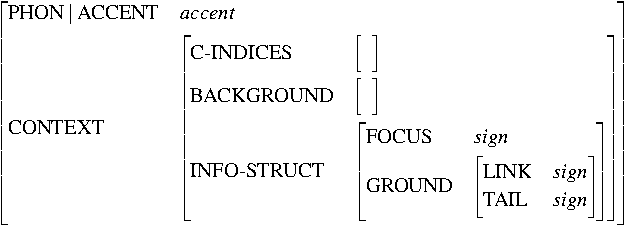
\includegraphics{pdf/engdahl-vallduvi.pdf}}}}

\myexe{\eenumsentence{\label{avm:engdahl:vallduvi:words}
\item\evnup{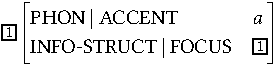
\includegraphics{pdf/engdahl-vallduvi-a.pdf}}
\item\evnup{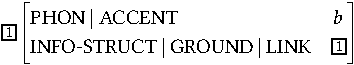
\includegraphics{pdf/engdahl-vallduvi-b.pdf}}
\item\evnup{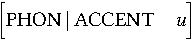
\includegraphics{pdf/engdahl-vallduvi-u.pdf}}}}


\citet{engdahl:vallduvi:96} regard information structure as an
interface across different layers in human language.  This notion can
be more precisely explained within the HPSG framework, because HPSG
accounts for various structural layers\is{HPSG} (e.g.\ phonology,
morphosyntax, semantics, and pragmatics) in an interactive
way. Regarding information structure in \ili{English},
\citeauthor{engdahl:vallduvi:96} pay particular attention to the
co-operation between phonological behaviors and contextual
information.  In their proposal, \tdl{accent} has three subtypes in
\ili{English}. They use the traditional distinction between the A and
B accents as shown in \myref{avm:engdahl:vallduvi:words}
\citep{bolinger:58,jackendoff:72}; \tdl{a} for A-accented words,
\tdl{b} for B-accented ones, and \tdl{u} for unaccented
ones.\is{A-accent}\is{B-accent} In order to determine if their
constraints work analogously cross-linguistically, they also analyze
sentences in Catalan, in which information structure is expressed
without reference to prosodic patterns. Unlike \ili{English}, Catalan
does not place a constraint on PHON to instantiate information
structure. INFO-STRUCT in Catalan, instead, is expressed via SUBCAT
(SUBCATegorization) and phrasal types of daughters.  Although their
analysis dwells on left/right \isi{dislocation} constructions in
Catalan, their approach has had a strong influence on following
HPSG-based studies, including \citet{dekuthy:00} for \ili{German},
\citet{bildhauer:07} for \ili{Spanish}, \citet{chang:02} and
\citet{chung:etal:03} for \ili{Korean}, \citet{ohtani:matsumoto:04}
and \citet{yoshimoto:etal:06} for \ili{Japanese}, and many
others.\is{HPSG}\is{left dislocation} \is{right dislocation}


These previous studies share a common proposal that information
structure is an independent module within a grammatical framework that
should be represented separately from CAT (CATegory) and CONT
(CONTent): Either under SYNSEM{$\mid$}CONTEXT
\citep{engdahl:vallduvi:96,chang:02,ohtani:matsumoto:04,yoshimoto:etal:06,paggio:09}
or outside of SYNSEM \citep{dekuthy:00,chung:etal:03,bildhauer:07}.
The current analysis, however, merges information structure into CONT
(i.e.\ MRS).\is{MRS}



On the other hand, previous studies are differentiated from each other
in the values the relevant types utilize in formalizing components of
information structure. In other words, it is necessary to determine
whether the value of the information-structure related features is a
whole sign or whether that value is something semantic
(i.e.\ MRS).\is{MRS} The traditional means of formalizing information
structure values is to use coreferences between the whole sign and a
value listed for FOC(US) and TOP(IC). \citet{engdahl:vallduvi:96} make
use of this method, and \citet{chung:etal:03} and
\citet{ohtani:matsumoto:04} utilize the same method for handling
information structure in Korean and Japanese, respectively. Recently,
several studies co-index something inside of MRS with a value in the
list of FOCUS, TOPIC, and others. In \citet{yoshimoto:etal:06},
\citet{bildhauer:07}, and \citet{sato:tam:12}, the RELS itself has a
structure-sharing with a value in the lists of components of
information structure.  \citet{paggio:09} also utilizes MRS,\is{MRS}
but the values in the lists of components of information structure are
co-indexed with the value of INDEX (e.g.\ \tdl{x1}, \tdl{e2}, etc.).
These two methods represent just two of many methods for representing
information structure in HPSG and MRS.\is{HPSG}\is{MRS} Taking a
different approach, \citet{chang:02} represents information structure
using just a string. \citet{kim:07} and \citet{kim:12a} use a boolean
feature as the value of FOCUS and TOPIC, and these features are under
an independent structure called INFO-ST.  Sometimes, a specific
feature structure is introduced, which represents logical forms
\citep{webelhuth:07,dekuthy:meurers:11}.


\subsection{Sentential forms}
\label{8:ssec:sform}


\citet{engdahl:vallduvi:96} argue that information structure is an
integral part of grammar.  In a similar vein, \citet{lambrecht:96}
regards information structure as a subtype of sentential grammar.


There exist various suggestions on how information structure affects
forms at the sentence level, such as topic-comment and
focus-\isi{ground} (i.e.\ bipartite structures).  There are two basic
components in the proposal by \citeauthor{engdahl:vallduvi:96};
\isi{focus} and \isi{ground}. While ground acts as an usher for focus,
focus is defined as the actual information or update potential of a
sentence. Ground, consisting of link and tail, is viewed as something
already subsumed by the input information state.\footnote{Note that
  ground is not the same as \isi{background}. Ground is thought of as
  opposite to focus, while background is neither focus nor
  \isi{topic}.}  This definition implies that a sentence can have a
ground if and only if the informative content guarantees its use. For
example, sentences with sentential focus (\tdl{all-focus} in 
the present study) -- such as a reply to
questions like \textit{What happened?}, are not required to include
ground.\is{background} Since they divide ground into link and tail, in
line with \citet{vallduvi:90}, they make use of a tripartite structure
consisting of different combinations of focus, link, and
tail.\footnote{\citet{buring:03} suggests another tripartite structure
  such as topic-focus-background.} Building upon some extra
constraints such as barring focus from preceding link (i.e.\ linear
order in instantiating information structure, such as link
\ensuremath{>} focus \ensuremath{>} tail), they propose four types of
sentential forms; link-focus, link-focus-tail, focus-tail, and
all-focus. For example, (\ref{exe:engdahl:vallduvi:96:5}A1) is a
link-focus construction, while (\ref{exe:engdahl:vallduvi:96:5}A2) is
a link-focus-tail construction.



\myexe{\enumsentence{\label{exe:engdahl:vallduvi:96:5}
\begin{tabular}[t]{ll}
Q1: & {So tell me about the people in the White House.} \\
    & {Anything I should know?}\\ 
A1: & {Yes. The \textbf{president} [$_{f}$ hates the
    Delft \textsc{chine set}]. Don't use it.}\\ Q2: & {In the
  Netherlands I got a big Delft china tray that matches the set}\\ & {in the
  living room. Was that a good idea?}\\ A2: & {Maybe. The
  \textbf{president} [$_{f}$ \textsc{hates}] the Delft chine set.} \\ & {(but
  the \textbf{first lady} \textsc{likes}
  it.) \citep[5]{engdahl:vallduvi:96}}\\
\end{tabular}}}


This classification is similarly implemented as a hierarchy in
\citet{paggio:09}, though the terms are different (i.e.\ \tdl{topic}
for link, and \tdl{bg} for tail). The type
hierarchy \citet[140]{paggio:09} proposes for \ili{Danish} is shown in
Figure~\ref{fig:hier:paggio}, and the lowest subtypes
are exemplified in \myref{exe:paggio} respectively.


 
\begin{figure}[!t]
\begin{center} 
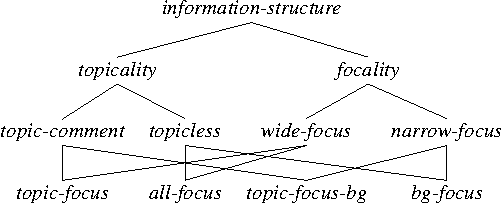
\includegraphics{pdf/paggio.pdf}
\caption{Type hierarchy of \citet{paggio:09}}
\label{fig:hier:paggio}
\end{center}
\end{figure}




\myexe{\eenumsentence{\toplabel{exe:paggio}
\item\shortex{8}
  {(Hvad & lavede & b{\o}rnene?) & [$_{T}$ & De] & [$_{F}$ & spiste & is].}
  {(what & did & children.\textsc{def}) & & they & & ate & icecream}
  {`What did the children do? They ate icecream.' (\tdl{topic-focus})}
\item\shortex{9}
  {(Hvad & spiste & b{\o}rnene?) & [$_{BG}$ & [$_{T}$ & De] & spiste] & [$_{F}$ & is].}
  {(what & ate & children.\textsc{def}) & & & they & ate & & icecream}
  {`What did the children eat? They ate icecream.' (\tdl{topic-focus-bg})}
\item\shortex{9}
  {(Hvem & har & spist & isen?) & [$_{BG}$ & Det & har] & [$_{F}$ & b{\o}rnene].}
  {(who & has & eaten & icecream.\textsc{def}) & & that & have & & children.\textsc{def}}
  {`Who has eaten the icecream? The children did.' (\tdl{bg-focus})}
\item\shortex{7}
  {(Hvad & skete & der?) & [$_{F}$ & B{\o}rnene & spiste]  & is].}
  {(what & happened & there) & & children.\textsc{def} & ate & icecream}
  {`What happened? The children ate icecream.' (\tdl{all-focus}) [dan] \citep[139]{paggio:09}}}}



The present study concurs that information structure needs to be
investigated as a subtype of sentential grammar
\citep{lambrecht:96,engdahl:vallduvi:96,paggio:09}. However, the type
hierarchy given in Figure~\ref{fig:hier:paggio} is altered in the
current analysis to accommodate a cross-linguistic perspective.  In
particular, it is necessary to delve into whether or not the hierarchy
for sentential forms has to deal with the linear order of components
of information structure.  At first glance, \tdl{bg-focus} in
Figure~\ref{fig:hier:paggio} might look inconsistent with the
focus-tail construction presented by
\citeauthor{engdahl:vallduvi:96}. As exemplified in
(\ref{exe:paggio}c), a constituent associated with \tdl{bg} can
precede other constituents associated with \tdl{focus} in
\ili{Danish}, which means the linear ordering constraint (i.e.\ link
\ensuremath{>} focus \ensuremath{>} tail) is language-specific.  The
different linear orders notwithstanding, the present study claims that
\tdl{bg-focus} in Figure~\ref{fig:hier:paggio} is actually the same as
focus-tail.  \citet{paggio:09} calls the identificational \isi{focus}
of (\ref{exe:paggio}c) \tdl{bg-focus} that serves to identify a
referent as the missing argument of an open proposition
\citep[122]{lambrecht:96}.\footnote{The \tdl{bg-focus} sentential form
  is similar to cleft constructions.\is{clefting}} For this reason,
the type hierarchy for sentential forms in the current work is built
up without an ordering constraint, exclusively considering which
components participate in forming information structure.






\subsection{Location within the feature geometry}
\label{8:ssec:hpsg:context}

Previous literature commonly introduces an independent typed feature
structure for information structure into \tdl{sign}. The independent
structure is either CXT (ConteXT) dealing with pragmatic
(i.e.\ contextual) information or just INFO-ST; \citet{chang:02}
employs PRA{$\mid$}DF{$\mid$}TFA in \myref{avm:chang:pra},
\citet{ohtani:matsumoto:04} uses CONX{$\mid$}INFO-ST, and
\citet{kim:07} uses just INFO-ST immediately under \tdl{sign}. Similar
structures are used in other papers:
SYNSEM{$\mid$}LOC{$\mid$}CONTEXT{$\mid$}INF-ST
\citep{yoshimoto:etal:06}, SYNSEM{$\mid$}IS \citep{bildhauer:cook:10},
CTXT{$\mid$}IS \citep{bjerre:11}, INFO-STRUC
\citep{dekuthy:meurers:11}, etc.  The functionality of these features
has one thing in common: Information structure is separately
represented from both morphosyntactic structure (i.e.\ CAT) and
semantic structure (i.e.\ CONT).




Information structure as presented here is an independent module in
grammar, however, that does not necessarily mean that information
structure should be separately represented on AVMs. Unless there is a
necessity to separate components of information structure from
CONT(ent), the independent structure is redundant.  In seeking a
minimal solution, is it possible to represent information structure
without introducing additional structure?  \citet{partee:91} also
addresses this with her observations that information structure is not
independent of truth-conditions.\is{truth-conditions} If information
structure is truth-conditionally relevant, it should be represented in
the semantics.  \citet{engdahl:vallduvi:96}, nevertheless, invoke
a separate representation in the belief that information structure and
logical semantics have to be represented in the grammar in a modular
manner. They leave the final resolution of these two components as a
question for future work.\is{HPSG} My understanding is that most
subsequent HPSG-based studies on information structure do not attempt
to answer how final meanings are arrived at.\footnote{To my knowledge,
  one exceptional study is \citet{webelhuth:07}, in which information
  structure components are dealt with under CONT.}  The next chapter
shows information structure can be fully represented without using
CTXT or introducing an independent structure.




Representing information structure within CONT (i.e.\ MRS)\is{MRS} has
another important merit in the context of multilingual machine
translation. As stated earlier, the present study argues that
translation means reshaping the packaging of the information of a
sentence.  Thus, one of the most important considerations in
representing information structure is its availability in multilingual
machine translation as a computational model. Because all ingredients
relevant to translation must be accessible in MRS within our
\isi{transfer-based} system \citep{oepen:etal:07}, information
structure should be accessible in MRS.




\subsection{Underspecification}
\label{8:ssec:underspecification}


One of the main motivations for and advantages in using the HPSG/MRS
formalism is \isi{underspecification}.  The value of a particular
attribute can be left underspecified in a description unless a
constraint identifies the value with a more specific type.  This makes
grammatical operation more flexible and more economical. For example,
(\ref{avm:engdahl:vallduvi:words}c) means that unaccented words leave
their information structure value underspecified, facilitating varied
meanings of an unmarked expression.\is{HPSG} \citet{kuhn:96} argues
that using \isi{underspecification} is a more effective way to
represent information structure; especially for the purpose of
implementing HPSG-based NLP applications (e.g.\ machine translation,
\isi{TTS} (Text-To-Speech) systems, etc.).  However,
underspecification has been scarcely used in previous HPSG-based
studies on information structure.  The current model relies on
underspecified values of components of information structure.  More
specific justifications as to why underspecification is crucial for
representing information structure are discussed in the following
subsections.


\subsubsection{Prosody}
\label{8:ssec:hpsg:prosody}

In most HPSG-based studies of information structure, a typed feature
structure for representing prosody is commonly introduced.\is{prosody}
The interface between information structure and prosody has been
studied for many Indo-European languages as well as in
non-Indo-European languages such as Korean and Japanese.
\myref{avm:chang:prosody}, taken from \citet{chang:02}, stands for a
typed feature structure for prosody in Korean which has two key
attributes TC (Terminal Contour) and STR (STRess). The values of the
former include falling (HL\%), neutral (H\%), and rising (LH\%), and
those of the latter stand for four levels of stress.



\myexe{\enumsentence{\label{avm:chang:prosody}\evnup{
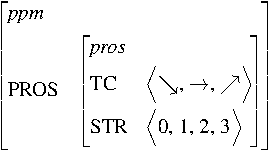
\includegraphics{pdf/chang-prosody.pdf}}}}

\noindent In his formalism, this structure has a correlation with
another typed feature structure, namely PRA (PRAgmatics). Information
structure values, such as topics and foci, are gathered into the lists
under PRA{$\mid$}DF{$\mid$}TFA as presented in
\myref{avm:chang:pra}\footnote{DF stands for Discourse Function, and
  TFA means Topic-Focus Articulation. Additionally, SA is short for
  Speech Act, BKG is for BacKGround, POV is for Point-Of-View, and CTR
  is for CenTeR.\is{background}}.

\myexe{\enumsentence{\label{avm:chang:pra}\evnup{
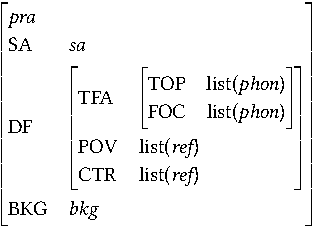
\includegraphics{pdf/chang-pra.pdf}}}}

\newpage 
\noindent For example, \nun and \ika in Korean have one of the feature
structures presented in (\ref{avm:chang:tf}a) and
(\ref{avm:chang:tf}b), respectively.  In \myref{avm:chang:tf}, the
PHON structure is the same as the STEM structure in
\texttt{matrix.tdl} of the \lingo \isi{Grammar Matrix} system. That is, the
value type of PHON is just string. Despite the name, it is not
directly related to any 
phonological information.\is{contrastive topic}\is{contrastive focus}\is{narrow focus}


\myexe{\enumsentence{\toplabel{avm:chang:tf} 
\begin{tabular}[t]{lllllll}
a. & i. & Zero Topic & & b. & i. & (Narrow) Focus \\ & &
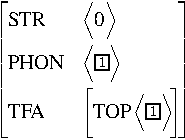
\includegraphics{pdf/chang-zt.pdf} & & & &
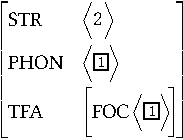
\includegraphics{pdf/chang-nf.pdf} \\ & ii. & (Thematic) Topic & & &
ii. & Contrastive Focus \\ & & 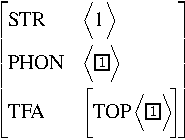
\includegraphics{pdf/chang-tt.pdf} & &
& & 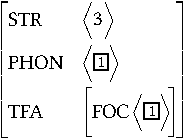
\includegraphics{pdf/chang-cf.pdf} \\ & iii. & Contrastive Topic
\\ & & 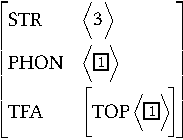
\includegraphics{pdf/chang-ct.pdf} \\
\end{tabular}}}




\noindent \citet{ohtani:matsumoto:04}, similarly, analyzed \wa-marked
and \ga-marked NPs in Japanese: \textit{Wa}-marked NPs are interpreted
as either \isi{topic}, restrictive \isi{focus} or non-restrictive
focus,\footnote{In \citet[95]{ohtani:matsumoto:04}, restrictive
  focus means wide focus.\is{wide focus}}  whereas \ga-marked NPs are interpreted as
either restrictive focus or all focus.  Similarly to
\myref{avm:chang:tf} in Korean, in the formalism
\citeauthor{ohtani:matsumoto:04} propose \wa and \ga can have one of
the feature structures in (\ref{avm:ohtani:matsumoto:wa:ga}a) and
(\ref{avm:ohtani:matsumoto:wa:ga}b), respectively.

\myexe{\enumsentence{\toplabel{avm:ohtani:matsumoto:wa:ga} 
\begin{tabular}[t]{lll}
a. & i. & \evnup{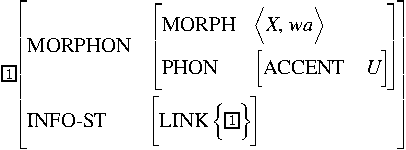
\includegraphics{pdf/ohtani-matsumoto-wa1.pdf}} \\
   & ii. & \evnup{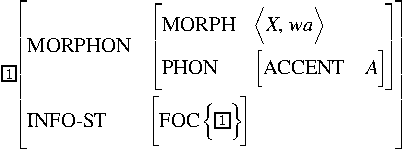
\includegraphics{pdf/ohtani-matsumoto-wa2.pdf}} \\
\end{tabular}
\newline
\begin{tabular}[t]{lllllll}
b. & i. & \evnup{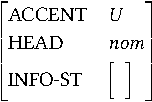
\includegraphics{pdf/ohtani-matsumoto-ga1.pdf}} &
ii. & \evnup{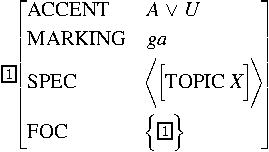
\includegraphics{pdf/ohtani-matsumoto-ga2.pdf}} \\
 & iii. &
\evnup{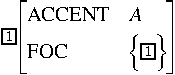
\includegraphics{pdf/ohtani-matsumoto-ga3.pdf}}
\end{tabular}}}



\myref{avm:chang:tf} and \myref{avm:ohtani:matsumoto:wa:ga}, though
their formats are slightly different, are actually the Korean and
Japanese variants of \myref{avm:engdahl:vallduvi:words} in
\ili{English}.  \citet{bildhauer:07} argues that it is rather unclear
where the information about accents comes from.  This criticism seems
appropriate when we think of the current computational environments
for sentence processing. Because our applications are mostly
text-based, for now it would be quite difficult to resolve for accent
type within the text domain. Nonetheless, the criticism seems rather
shortsighted when we consider the future direction of language
applications.\is{HPSG} Even in the absence of an implementation that
connects the HPSG grammar to ASR (Automatic Speech Recognition)
systems to prosody extraction or \isi{TTS} (Text-To-Speech) systems
with prosody generation,\is{prosody} if there is a robust correlation
between information structure and prosodic accents, the grammar can
leverage information about stress to yield higher performance. Hence,
it is important to allow the grammar formalism to model prosodic
information using \isi{underspecification} \citep{kuhn:96}. I believe
that this strategy contributes to the long-term task of refining
meaning representation via prosodic information.



However, there is a remaining controversial point embedded in
\myref{avm:chang:tf} and \myref{avm:ohtani:matsumoto:wa:ga}.  In fact,
they are tantamount to redundantly introducing \ika and \nun in
Korean, and \ga and \wa in Japanese into the lexicon. For example,
(\ref{avm:chang:tf}a) implies that the morphemes for introducing a
zero \isi{topic} \nun, a thematic topic \nun, and a \isi{contrastive
  topic} \nun are three separate homonyms.  The use of multiple rules
for \nun and \wa is an undesirable choice which should be avoided if
possible.  Korean and Japanese very productively employ \nun and \wa,
respectively, which means that having multiple lexical entries for \wa
and \nun items in the respective grammars causes problematic amounts
of spurious ambiguity.\footnote{Exploring the \textit{Sejong} Korean
  Treebank reveals that subjects in Korean are combined with \nun more
  than twice than the ordinary nominative marker \ika.} In other
words, if we include all the rules in (\ref{avm:chang:tf}a), every
\onun-marked constituent produces spurious parse trees.  As a result,
the number of parse trees can sometimes grow too large to
handle.\footnote{In fact, this is one of the major problems that cause
  a bottleneck in parsing and generation in the old version of Korean
  Resource Grammar.  It had two types of \nun; one for topic, and the
  other for contrast.\is{contrast} These two \nun sometimes had an
  adverse effect on system performance.  Occasionally, even not a long
  sentence could have a large number of parse trees if \nun occurs
  multiple times in the sentence. Accordingly, the sentence could not
  be generated in most cases because of memory overflow. For more
  information, see \citet{song:etal:10}.}  If there is something that
the multiple-entry approach captures that the single-entry approach
does not, then we should use the former, because there could be a loss
in information processing. Yet, as discussed hitherto, the lexical
markers (e.g.\ \nun and \wa) and the prosodic patterns each contribute
only partial information. In other words, neither of them can be a
decisive clue for identifying which information structure meaning is
assigned to a given constituent.



To sum up, my alternate approach for constraining lexical markers
(especially in Japanese and Korean) is as follows:\is{lexical markers}
First, there is one and only one entry for each marker. Second, the
lexical rules include prosodic structures in principle, but they are
preferentially underspecified. Third, the meaning that each marker
potentially conveys is flexibly and tractably represented to cover all
the partial information.



\subsubsection{Ambiguity}
\label{8:ssec:hpsg:boolean}


In many previous studies across theories of grammar, so-called
F(ocus)-marking is represented as a boolean feature (i.e.\ [FOCUS
  \tdl{bool}]) as proposed in \citet{zubizarreta:98}.  Handling
information structure via a boolean feature is also common in other
unification-based frameworks. For instance, \citet{choi:99}, within
the framework of \isi{LFG} (Lexical-Functional Grammar
\citealt{bresnan:01}), makes use of [\ensuremath{\pm} New] and
[\ensuremath{\pm} Prom] as presented later in \myref{fig:choi}.  Other
components of information structure are also similarly marked.  These
include [TOPIC \tdl{bool}], [CONTRAST \tdl{bool}], [HIGHLIGHT
  \tdl{bool}], and so on. For instance, \citet{kim:07} claims that
\textit{beer} in (\ref{exe:kim:beer}A) is constrained as in
\myref{avm:kim:beer}. Since \textit{beer} in (\ref{exe:kim:beer}A)
is contrastively focused (i.e.\ an answer to an alternative question
\citealt{gryllia:09}),\is{contrastive focus} it has both [HIGHLIGHT +]
and [FOCUS +] in his analysis. Note that [HIGHLIGHT \tdl{bool}] in
\myref{avm:kim:beer} indicates whether or not the constituent conveys
a contrastive meaning, which is almost the same as [CONTRAST
  \tdl{bool}].


\myexe{\enumsentence{\label{exe:kim:beer}
\begin{tabular}[t]{ll}
Q: & {Did John drink beer or coke?}\\ 
A: & {John drank beer. \citep[229]{kim:07}}\\
\end{tabular}}}

\myexe{\enumsentence{\label{avm:kim:beer}\evnup{
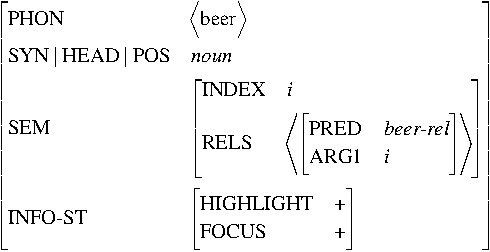
\includegraphics{pdf/kim-beer.pdf}}}}


In contrast, the present work does not use boolean features for
representing information structure meaning. This is mainly because
using boolean features would not allow us to represent information
structure as a relationship between an entity and a clause. The
current work encodes information structure into the semantic
representation via \isi{ICONS} (Individual CONStraints).\is{Individual CONStraints}
The main motivation for \isi{ICONS} is the ability to
encode information structure values as a relationship with the clause
an information structure-marked constituent belongs to, rather than as
simply a property of the constituent itself.  Chapter~\ref{chapter9}
provides the fundamentals of \isi{ICONS} in detail.




\subsection{Marking \vs Meaning}
\label{8:ssec:hpsg:makring-meaning}

Most of the previous formalisms are exclusively concerned with
markings, as the name F(ocus)-marking implies.  Hence, they are rather
ill-suited to deal with any discrepancies between the forms expressing
information structure and the meanings expressed.\is{lexical markers}
The lexical markers \wa and \nun in Japanese and Korean are typical
cases showing this kind of mismatch, and \myref{avm:kim:beer}
illustrates via an example from Korean.  If \nun in Korean is used
contrastively and an NP with it is focused,\is{contrast} then the NP in
\citeauthor{kim:07}'s AVMs would be constrained as either (i) [HIGHLIGHT +,
  TOPIC +] focusing on the NP-marking system or (ii) [HIGHLIGHT +,
  FOCUS +] putting more weight on the meaning. Another potential
constraint on the NP would be [HIGHLIGHT +, FOCUS +, TOPIC +], but
this analysis fails with respect to the basic assumption the present
study is built on: topic and focus are mutually exclusive.\footnote{As
  stated earlier, there exist counterarguments to this generalization
  \citep{krifka:08}.}



The present study proposes two strategies as an alternative method.
First, information structure markings should be separately specified
from information structure meanings. The former should be constrained
using a morphosyntactic feature that can be language-specific. The
latter should be attributed within the semantics (i.e.\ under CONT),
and rely on a cross-linguistically valid type hierarchy. Second, there
are more than a few cases in which we cannot convincingly say which
element is associated with which information structure meaning.
Therefore, it is necessary to specify information structure values as
flexibly as possible. This is particularly important when creating a
robust computational model of information structure.




\section{Information structure in MRS}
\label{8:sec:mrs}


The present study, unlike previous HPSG-based studies including
\citet{engdahl:vallduvi:96}, does not introduce another structure and
instead represents information structure within the MRS semantic
representations.\is{MRS} There are two motivations for doing so. The
first motivation is that information structure impacts semantic
properties. As discussed previously, information structure
(especially, semantic \isi{focus}) is sometimes relevant to
\isi{truth-conditions} \citep{gundel:99} and scopal interpretation
\citep{buring:97,portner:yabushita:98,erteschik:99,erteschik:07,bianchi:frascarelli:10}.
Hence, it is right to incorporate information structure into the
meaning representation in a direct manner.  The second motivation is
strictly practical: The \isi{infrastructure} for machine translation
does MRS-based transfer \citep{oepen:etal:07}, therefore encoding
information structure into MRS facilitates its immediate availability
for use in machine translation.\is{transfer-based}




Previous HPSG-based studies can be divided into two subgroups: One
represents information structure without reference to MRS
\citep{dekuthy:00,chang:02,chung:etal:03,ohtani:matsumoto:04,webelhuth:07,kim:07,kim:12a},
and the other links information structure values in an independent
typed feature structure to MRS (e.g.\ INDEX or RELS)
\citep{wilcock:05,yoshimoto:etal:06,paggio:09,bildhauer:cook:10,sato:tam:12}.



\citet{wilcock:05}, to my knowledge, is the first attempt to use MRS
for representing information structure, modeling the scope of
\isi{focus} analogously to \isi{quantifier} scope
(i.e.\ HCONS).\is{MRS}


\myexe{\eenumsentence{\label{exe:wilcock}
\item{The president [$_{f}$ hates the china set].}
\item{1:the(x,2), 2:president(x), 3:the(y,4), 4:china(y), 4:set(y),
  5:hate(e,x,y)\\ TOP-HANDLE:5, LINK:{1}, FOCUS:{3,5} (wide focus)}}}



\noindent This is similar to the basic idea of the current analysis,
in that information structure can be represented as a list of binary
relations in the same way as HCONS is.\is{binary relation} The
difference between \citeauthor{wilcock:05}'s proposal and that of the
current analysis is that information structure in his model is
represented as handles, whereas the current model represents the
relationships between individuals and clauses as binary
relations. This facilitates scaling to multiclausal constructions. For
instance, (\ref{exe:wilcock}b) taken from \citet[275]{wilcock:05}
represents the wide \isi{focus} reading of (\ref{exe:wilcock}a)
(i.e.\ from 3 to 5). Note that in this representation, LINK
(\tdl{topic} in this paper) and FOCUS have no relation to the clause
or its head (\textit{hate}).\is{topic}





\citet{yoshimoto:etal:06} use MRS,\is{MRS} too. In their model,
information structure values are unified with whole MRS predications
rather than just indices. Based on this assumption, they apply the
information structure values to analyzing floating quantifiers in
Japanese.  However, their AVM does not look like a standard MRS
representation, and it is rather unclear how their model could be used
for practical purposes.



\citet{paggio:09} also models information structure with reference to
the MRS formalism, but the components of information structure in
\citeauthor{paggio:09}'s proposal are represented as a part of the
context, not the semantics. Though each component under
CTXT\ensuremath{\mid}INFOSTR involves co-indexation with individuals
in MRS, her approach cannot be directly applied to the \isi{\logon} MT
\isi{infrastructure} which requires all transfer-related ingredients
to be accessible in MRS \citep{oepen:etal:07}.



\citet{bildhauer:cook:10} offer another type of MRS-based
architecture:\is{MRS} Information structure in their proposal is
represented directly under SYNSEM (i.e.\ SYNSEM\ensuremath{\mid}IS)
and each component (e.g.\ TOPIC, FOCUS) has a list of indices
identified with ones that appear in EPs in RELS, which is not
applicable to the \isi{\logon} \isi{infrastructure} for the same
reason as the \citet{paggio:09} model.\footnote{This, of course, does
  not mean that every grammar should be compatible with the
  \isi{\logon} infrastructure. The ultimate goal of the present study
  is creating a computational library within the Grammar Matrix, which
  can be effectively used to enhance performance of HPSG/MRS-based MT
  systems. Given that \isi{\logon}, for now, is the readily available
  infrastructure for the purpose, the present study follows the
  requirements as far as possible.}



Among the various methods presented so far, the method used by the
present study most closely resembles that of \citet{paggio:09} in that
individuals (the value type of INDEX) are constrained for
representation of information structure (i.e.\ Individual
CONStraints).\is{Individual CONStraints} The main differences between
\citeauthor{paggio:09}'s approach and mine are as follows: First, I
place the feature whose value represents information structure inside
of CONT. Second, I represent information structure values using a type
hierarchy of \tdl{info-str}.\is{\textit{info-str}} Third, the features
to represent information structure involve a \isi{binary relation}
between individuals and clauses. Chapter~\ref{chapter10} enters into
the implementation details.




\section{Phonological information in HPSG}
\label{8:sec:phonology}

Quite a few HPSG-based studies explore the effect of phonological
behaviors on the structuring of information in a sentence.  However,
this subsection surveys only \citeauthor{bildhauer:07}'s
proposal.\is{HPSG}


Though the current model does not devote much attention to
phonological constraints on information structure, it is still
necessary to formalize some prosodic information in relation to
information structure markings for at least two reasons. First,
\isi{focus projection} has been considered to be triggered by
prosody. Second, as \citet{kuhn:96} and \citet{traat:bos:04} point
out, \isi{TTS} (Text-To-Speech) synthesizers and automatic speech
recognizers can be improved by using information structure. Thus, it
is my expectation that including prosodic information in the HPSG
formalism facilitates the use of HPSG-based grammars for those kinds
of systems in the long term.



According to the account of \citet{bildhauer:07}, there are three
HPSG-based approaches to phonology; (i) metrical tree-based approaches
\citep{klein:00,haji:03}, (ii) grid-only approaches
\citep{bonami:delais:06}, and (iii) hybrid approaches that take
advantage of the two former approaches (\citeauthor{bildhauer:07}'s
own).  According to \citet[160]{bildhauer:07}, the metrical tree-based
approach provides a representation of prosodic consistency, but
deploys only nested structure. This is a drawback when it comes to
handling intonational tunes.  \citeauthor{bildhauer:07} also argues
that while the grid-only approach of \citeauthor{bonami:delais:06}
involves a basically flat representation, it is too language-spe\-cif\-ic
to be straightforwardly applied to other languages. The three basic
approaches outlined by \citeauthor{bildhauer:07} each yield their own
explanation about how phonological information can be calculated
within the HPSG framework in a general sense, and how the information
co-operates with information structure.


Another approach to the HPSG-based interface between prosody and
syntax is provided in \citet{yoshimoto:00}.\is{prosody} Its basic
assumption is that P(rosodic)-structure and C(onstituent)-structure
form a bistratal phase with each other. The bistratal approach is not
considered in the present study for two reasons. First,
\citeauthor{yoshimoto:00}'s proposal is not directly concerned with
information structure. Second, although the interaction between
prosodic and syntactic structures is examined, the analysis is rather
language-specific (i.e.\ for Japanese) as implied by the name of the
typed feature that plays the key role (MORA).



The present analysis, largely accepting the hybrid approach, keeps an
eye towards being compatible with the HPSG-based formalism
\citet{bildhauer:07} proposes.  \citeauthor{bildhauer:07}'s account is
divided into two layers. One is the PHON list which is an immediate
feature of \tdl{sign}, made up of four components; (i) prosodic word,
(ii) phonological phrase, (iii) intonational phrase, and (iv)
phonological utterance. The other layer is intonation, which takes
charge of (v) pitch accents,\is{focus prominence} and (vi) boundary
tones. Building upon their operation, a schema of \isi{focus} prominence
rules is suggested, mainly concentrating on the top level of prosodic
hierarchy (i.e.\ phonological utterance). \citeauthor{bildhauer:07}'s
formalism develops from \citeauthor{klein:00}'s proposal that the
level of syllables does not matter, and instead the prosodic hierarchy
is represented by prosodic words (\tdl{pwrd}) and leaners
(\tdl{lnr}). The elementary unit of PHON is \tdl{pwrd}, whose skeleton
is sketched out in \myref{fig:bildhauer:pwrd-or-lnr}
\citep[161]{bildhauer:07}.\footnote{In
  \myref{fig:bildhauer:pwrd-or-lnr}, the value of SEGS is a list of
  segments.}

\myexe{\enumsentence{\label{fig:bildhauer:pwrd-or-lnr}\evnup{
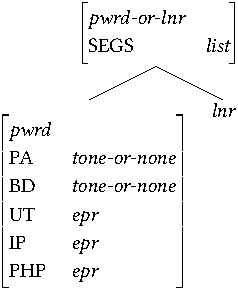
\includegraphics{pdf/pwrd-or-lnr.pdf}}}}

\newpage 
First, the lowest three features within \tdl{pwrd} in
\myref{fig:bildhauer:pwrd-or-lnr} represent prosodic hierarchical
levels above prosodic word; PHP stands for PHonological Phrase, IP is
for Intonational Phrase, and UT is the abbreviation for phonological
UTterance. Each of them has \tdl{epr} meaning Edges and Prominence as
its value type, whose typed feature structure is provided in
\myref{fig:bildhauer:epr}; LE stands for Left Edge, RE for Right Edge,
and most importantly DTE for Designated Terminal Element. Grounded
upon the prosodic rules that \citet[181]{bildhauer:07} creates, PHP, IP,
and UT are defined by a relational constraint, which places a
restriction on LE, RE, and DTE values of \tdl{pwrd} objects and
thereby specifies the relation that a prosodic word has to higher
prosodic constituents.



\myexe{\enumsentence{\label{fig:bildhauer:epr}\evnup{
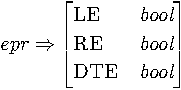
\includegraphics{pdf/epr.pdf}}}}


Second, pitch accents (PA) and boundary tones (BD), which carry
intonational information, take \tdl{tone-or-none} as their value
type. \citet[183--184]{bildhauer:07} provides the hierarchy of
\tdl{tone-or-none} in \ili{Spanish} as follows, which is to be further
revised for better cross-linguistic coverage in the present study.
Each type name on the bottom line is an element in the ToBI
format. For example, \tdl{high} means H, \tdl{low} means L, and
\tdl{low-high-star} means L+H* (i.e.\ the B-accent in \ili{English},
\citealt{bolinger:61,jackendoff:72}).\is{B-accent}


\myexe{\enumsentence{\label{fig:bildhauer:tone-or-none}\evnup{
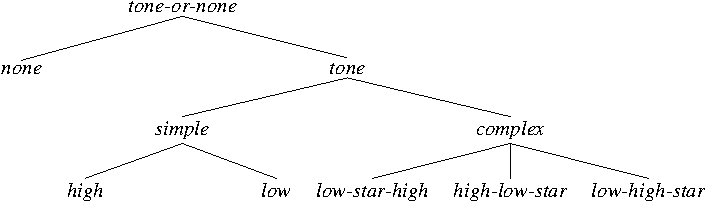
\includegraphics[width=.9\textwidth]{pdf/tone-or-none-spa.pdf}}}}


\noindent Those pitch accents and boundary tones are related to
\tdl{pwrd}, whose relationship is ruled as follows.  Pitch accents are
attached to phonological phrases, and boundary tones are connected to
intonational phrases \citep{steedman:00}.


\newpage 
\myexe{\eenumsentence{\label{avm:bildhauer:rules}
\item\evnup{{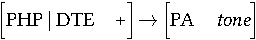
\includegraphics{pdf/php-plus.pdf}}}
\item\evnup{{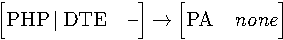
\includegraphics{pdf/php-minus.pdf}}}
\item\evnup{{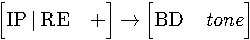
\includegraphics{pdf/ip-plus.pdf}}}
\item\evnup{{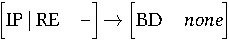
\includegraphics{pdf/ip-minus.pdf}}}}}



Given that \citet{bildhauer:07} provides a cross-linguistically
convincing proposal as such, the type hierarchy of \tdl{tone} and the
typed feature structure for phonological structure are described in
\texttt{matrix.tdl}.  Although the current work is not deeply
concerned with prosodic realizations of information structure,
information relevant to those realizations should be included into the
system as it's a common structure in human languages. This is highly
motivated by the necessity to refer to prosodic patterns for further
refinement of meaning representation in future studies.



However, the specific phonological rules given in
\myref{avm:bildhauer:rules} are only selectively implemented in the
current work. For instance, in the following chapters, two
hypothetical suffixes are used for indicating the A and B accents in
\ili{English} for ease of processing.  The rules for them are in
accordance with what \citet{bildhauer:07} proposes. However, no other
rules use that phonological information. There are two reasons for
this.\is{prosody} First, for many languages, the correlation between
prosody and information structure is not fully tested and thereby
remains unclear. Thus, I leave it to future users of the current model
to create these (potentially language-specific) rules. Second, since
the current model does not make use of any acoustic system, it is
almost impossible for the current model to implement and test
\citeauthor{bildhauer:07}'s phonological rules in a comprehensive way.

 \largerpage[-1]
\section{Information structure in other frameworks}
\label{8:sec:other-frameworks}


\subsection{CCG-based studies}
\label{8:ssec:ccg}

The \isi{CCG} (Combinatory Categorial Grammar, \citealt{steedman:01})
framework, which provides a detailed analysis of the relationship
between intonation and other structures (e.g.\ syntax, semantics, and
pragmatics), has addressed information structure since the early days
of the theory \citep{steedman:00}.\footnote{CCG departing from CC
  (Categorial Grammar) has two versions of formalism, whose history of
  progress is also deeply related to incorporating information
  structure into the formalism. The first development of CG theories
  is called UCG (Unification Categorial Grammar, \citealt{zeevat:87}),
  which employs an HPSG-style typed feature structures
  (i.e.\ \tdl{sign}). The HPSG-style formalism facilitates more
  efficient co-operation of interface across grammatical layers
  (e.g.\ syntax, semantics, etc.). The second development is UCCG
  (Unificational Combinatory Categorial Grammar,
  \citealt{traat:bos:04}), which integrates CCG and UCG, and then adds
  DRT (Discourse Representation Theory, \citealt{kamp:reyle:93}) into
  the formalism, in order to facilitate a compositional analysis of
  information structure.  Roughly speaking, those categorial grammars
  replace phrasal structure rules by lexical categories and general
  combinatory rules. In other words, the CCG framework associates
  syntactically potent elements with a syntactic category that
  identifies them as functors. There are two major rules to combine
  functional categories and their arguments, which specify
  directionality such as (i) forward application represented as
  `\ensuremath{>}' and (ii) backward application represented as
  `\ensuremath{<}'.} Consequently, one of the main characteristics of
CCG is that it is particularly and deeply oriented toward information
structure. Moreover, several CCG-based studies have accounted for how
categories of information structure in CCG can be of use for practical
systems from the standpoint of computational linguistics.


The components of information structure that \citet{steedman:00} and
\citet{traat:bos:04} introduce include theme (i.e.\ \isi{topic}), and rheme,
and \isi{focus}. There are three structures that coincide with each other:
(a) surface structure, (b) information structure, and (c) intonation.
Among these, only (c) has significance for combinatory prosody,
consisting of (c-1) pitch accents and (c-2) boundary tones. Whereas
pitch accents are viewed as properties of words, boundary tones are
defined as a boundary between theme and rheme categories.  A sequence
of one or more pitch accents followed by a boundary is referred to as
an intonational phrasal tune.


\largerpage
Pitch accents and boundary tones in CCG are mostly represented in the
ToBI format as follows.  There are six pitch accents to mark theme and
rheme, for example L+H*, L*+H for theme and H*, L*, H*+L, and H+L* for
rheme. Boundary tones are what make a clear difference between
\citeauthor{steedman:00}'s analysis and others in that he considers
them to be crucial to specifying phrasal type and thereby configuring
information structure.  Intermediate phrases consist of one or more
pitch accents, followed by either the L or the H boundary, also known
as the phrasal tone. Intonational phrase, on the other hand, consists
of one or more intermediate phrases followed by an L\% of H\% boundary
tone. Therefore, in \citeauthor{steedman:00}'s analysis of information
structure in \ili{English}, the L+H* and LH\% tune is associated with
the theme, and the H* L and H* LL\% tunes are associated with the
rheme. For instance, a surface structure \textit{Anna married Manny.}
can be analyzed as follows \citep[302]{traat:bos:04}.



\myexe{\eenumsentence{\toplabel{exe:traat:bos:04}
\item \textbf{Anna} [$_{f}$ married [$_{f}$ \textsc{Manny}]].
\item Anna L+H* LH\% married Manny H* LL\%}}


\noindent In (\ref{exe:traat:bos:04}a), \textbf{Anna} bears the
B-accent (i.e.\ L+H*), \textsc{Manny} bears the A-accent (i.e.\ H*),
and the \isi{focus} can be projected into either the NP \textsc{Manny}
itself or the VP \textit{married
  \textbf{Manny}}.\is{A-accent}\is{B-accent} In
(\ref{exe:traat:bos:04}b), the \isi{topic} meaning that
\textit{\textsc{Anna}} conveys comes from a pitch accent (L+H* after
the word), and the focus meaning that \textit{\textbf{Manny}} delivers
comes from another pitch accent (H*). A boundary tone (LH\%) forms a
border of theme. Finally, \textit{married} without any boundary tone
(i.e.\ an invisible boundary as an edge of an unmarked theme) is
included in the rheme, but it creates an ambiguous meaning with
respect to the \isi{focus} domain. \citet{traat:bos:04} represent
(\ref{exe:traat:bos:04}b) into the CCG-based formalism, in which three
information structure values \ensuremath{\theta}, \ensuremath{\rho},
and \ensuremath{\phi} are used for theme, rheme, and phrase,
respectively. Those values are used as the value types of INF
(INFormation structure), and focus is independently represented as a
boolean type.



The CCG-based studies have several key implications for my
work. First, they pay particular attention to the creation of a
computational model for information structure with an eye toward
implementing applications from the beginning.  In particular,
\citet{traat:bos:04} argue that an information structure-based
computational model should be used for both parsing and generation,
and conduct an experiment to verify that their model works.  The
information structure-based model used here was created with the same
considerations in mind. This computational model, developed in the
context of \isi{grammar engineering}, can be used not only for parsing
human sentences into semantic representations but also for generating
sentences using that representation.  Second,
\citeauthor{traat:bos:04} make use of prosodically annotated strings
as input for their experiment, because current automatic speech
recognizers do not provide enriched prosodic information.  In the
current experiment, I employ two suffixes (e.g.\ 	\textit{-a} for the
A-accent, 	\textit{-b} for the B-accent) that hypothetically represent
prosodic information (see Section \ref{12:sec:machinery}).  Though I am not
working with naturally occurring speech, the 	\textit{-a} and 	\textit{-b} suffixes
are inspired by prosodic annotation.  Lastly, the CCG-based studies
include prosodic information in their formalism in a fine-grained way
and also create linguistic rules in which prosodic information and
information structure interact with each other in a systemic way.  My
model does not yet fully use prosodic information for the reasons
discussed in Section \ref{8:sec:phonology},\is{prosody} but future work will
look at how to systematize the interaction between prosody and
information structure, taking CCG-based work as a starting point and
guide.  Although the current model is mainly concerned with text
processing, it could work through acoustic analysis of speech, through
pre-tagging of information structure, and/or through mark-up like
\textbf{boldface} or \textsc{all caps}.





\subsection{LFG-based studies}
\label{8:ssec:lfg}
\largerpage


While most HPSG/CCG-based studies on information structure emphasize
the interaction between phonological factors and morphosyntactic
structures,\is{HPSG}\is{CCG} previous studies based on \isi{LFG} tend
to be more concerned with morphosyntactic operation.\footnote{The
  Lexical-Functional Grammar framework, as the name itself implies,
  has two motivations: (i) Lexical items are substantially structured,
  and (ii) grammatical functions (e.g.\ subject and object) play an important role.
 LFG assumes several structural layers in the analysis
  of language phenomena, which include c-structure (constituent
  structure), and f-structure (functional structure). C-structure
  converts overt linear and hierarchical organization of words into
  phrases with non-configurationally structured information about
  grammatical functions, which plays a role to form
  f-structure. F-structure refers to abstract functional organization
  of the sentence, (e.g.\ syntactic predicate-argument structure and
  functional relations), which is of help in explaining universal
  phenomena in human language. In addition to the two basic
  structures, several other structures are also hypothesized such as
  a-structure (argument structure), s-structure (semantic structure),
  m-structure (morphological structure), p-structure (phonological
  structure), and i-structure (information structure).}
Discourse-related information is largely represented in LFG either
within an independent structure (i.e.\ i-structure) \citep{king:97} or
just inside of f-structure \citep{bresnan:01}.



It is my understanding that the first endeavor to study linguistic
phenomena related to information structure within the LFG framework is
offered in \citet{bresnan:mchombo:87}. Grammatical functions in LFG
can be roughly divided into discourse functions and non-discourse
functions.  In their analysis, grammaticalized discourse functions
such as TOP(ic) and FOC(us) are captured within f-structure.



The practice of putting information structure elements into
f-structure, however, is potentially controversial, because
information structure does not always coincide with grammatical
functions such as OBJ(ect), COMPL(ement), and so forth
\citep{king:zaenen:04}. In order to overcome potential problems
related to this, \citet{king:97} introduces i-structure to represent
how information structure units (e.g.\ \isi{focus} domain) are
constructed. In other words, i-structure can be represented
independently of morphosyntactic operation, thereby disentangling
information structure forms and meanings.  Several subsequent
LFG-based studies such as \citet{choi:99} and \cite{man:07} are in
line with \citeauthor{king:97}. While \citeauthor{king:97} is mainly
concerned with \ili{Russian}, the following studies adapt i-structure
to other languages and substantiate its feasibility within the LFG
framework. These include, \ili{Korean} \citep{choi:99}, \ili{German}
\citep{choi:99}, and \ili{Cantonese} \citep{man:07}.



Another characteristic of LFG-based studies for information structure
uses two types of boolean features which constrain information status
such as new/given and prominent/non-prominent. This distinction is
proposed in \citet{choi:99}, who classifies (i) \isi{focus} into (i-a)
completive focus involving new information and (i-b) \isi{contrastive focus}
entailing alternatives in a set,\is{alternative set} and makes a
clear-cut distinction between (ii) \isi{topic} and (iii) tail using
[\ensuremath{\pm} prominent]. \citeauthor{choi:99}'s cross-classification between them is
sketched out in \myref{fig:choi}.\footnote{In
  \myref{fig:choi}, Prom is short for Prominence.}
\citeauthor{choi:99} applies this classification to the representation
of information structure in \ili{Korean}, and \citet{man:07} applies
it to \ili{Cantonese} in almost the same way.

\myexe{\enumsentence{\label{fig:choi}\evnup{
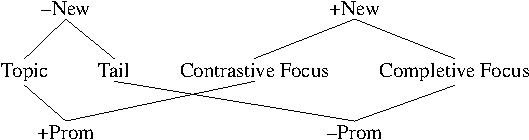
\includegraphics{pdf/choi.pdf}}}} 



Though the underlying framework is different, these LFG-based studies
also have implications for the current model.  First of all,
\citet{bresnan:mchombo:87} provides an analysis of information
structure in multiclausal utterances. They delve into how \isi{topic}
relations in \ili{English} and Chiche{\^w}a can be captured in several
types of multiclausal constructions such as embedded clauses, relative
clauses, and cleft clauses.\is{clefting} This highlights the
importance of capturing an information structure relation between a
subordinate clause and the main clause that the subordinate clause
belongs to. In other words, subordinate clauses constitute their own
information structure, but the relation to their main clauses
additionally needs to be represented with respect to information
structure.  This is discussed in more detail in Section \ref{9:ssec:binary}
and Section \ref{10:ssec:relative:background}.  Second, LFG-based studies deal
with a variety of constructions in the study of information structure,
whereas a large number of studies based on other frameworks treat only
simple declarative sentences. The construction types that LFG-based
studies address include interrogatives
(\textit{wh}-questions\is{\textit{wh}-questions} and
\textit{yes}/\textit{no}-questions), negation,\is{negation} clefts
\citep{king:95}, \isi{scrambling} \citep{choi:99}, and so-called
topicalization (i.e.\ \isi{focus}/topic \isi{fronting} in the present study)
\citep{man:07}.  Third, it is also noteworthy that LFG-based studies
tend to apply their formalism directly within a specific
language. Studies within other frameworks normally apply their
formalisms to \ili{English} first, and then project them analogously
into other languages. As a consequence, the analyses tend to be rather
dependent on English-like criteria. LFG-based work, on the other hand,
straightforwardly looks into how a language configures information
structure. LFG-based work on information structure has sometimes been
criticized for not treating prosodic factors significantly, but to my
understanding this is mainly because they do not start their work from
English, and as we have seen,\is{prosody} prosody is not heavily
responsible for information structure markings in a number of
languages (e.g.\ \ili{Chiche{\^w}a}, \ili{Korean}, and
\ili{Cantonese}).  Fourth, LFG-based studies take significant notice
of the mismatches between meanings and markings of information
structure and seek to reflect these discrepancies in their
formalism. Lastly, the present model is similar to
\citet{bresnan:mchombo:87} in that information structure is handled
within SYNSEM and an independent structure is therefore not needed.



\section{Summary}
\label{8:ssec:summary}

Since the pioneering work of \citet{engdahl:vallduvi:96}, information
structure has received attention in HPSG-based research.  The main
endeavor of these studies is to point out the necessity of viewing
sentential form in relation to information structure. This motivation
is also importantly applied to my model. Nevertheless, the present
study differs from previous studies in several key ways. First,
\isi{underspecification} is not widely used in the previous studies,
but the current model emphasizes underspecification as a key to the
representation of information structure. Second, while most previous
studies do not differentiate information structure marking and
information structure meaning, the two are entirely distinct in the
current model. Third, information structure is represented only under
CONT(ent) (i.e.\ MRS)\is{MRS} in the current model rather than in a
separate structure. Fourth, prosodic information is selectively
incorporated into the formalism, in accordance with what
\citet{bildhauer:07} suggests from a big picture perspective, but with
the direct application of his specific rules.  The implementation
details are discusses in the following chapters in addition to several
interesting points proposed in other frameworks. In particular,
inspired by the LFG-based studies, Chapter~\ref{chapter10-2} delves
into information structure with special reference to various types of
utterances (i.e.\ multiclausal constructions).


\chapter{Individual CONStraints: fundamentals}
\label{chapter9}
\setcounter{enums}{0}


\noindent The present study suggests the use of ICONS (Individual
CONStraints) as the key means of representing information structure
within the framework of HPSG\is{HPSG} (\citealt{pollard:sag:94}) and
MRS\is{MRS}\is{Individual CONStraints}
(\citealt{copestake:etal:05}).\footnote{The feature \isi{ICONS} was
  originally proposed by Ann Copestake and Dan
  Flickinger,\ia{Copestake, Ann}\ia{Flickinger, Dan} for the purpose
  of capturing semantically relevant connections between individuals
  which are nonetheless not well modeled as elementary predications,
  such as those found in intrasentential anaphora, apposition, and
  nonrestrictive relative clauses.\is{relative clause} Copestake and
  Flickinger suggested that the same mechanism can be used to anchor
  information structure constraints to particular clauses.  In a more
  general system that uses ICONS, the value of \isi{ICONS} would be a
  list of items of type \tdl{icons}, where \tdl{info-str} is a subtype
  of \tdl{icons}.\is{\textit{info-str}} For instance, \citet{song:16}
  represents honorification as a binary relation between referential
  items in dialogue via ICONS.} Section \ref{2:sec:mrs} goes over the basic
skeletons of Minimal Recursion Semantics.  Section \ref{9:sec:motivations}
offers the basic necessities for using \isi{ICONS} in processing
information structure. Section \ref{9:sec:info-str}, Section \ref{9:ssec:mkg}, and
Section \ref{9:ssec:sform} propose three type hierarchies that place
constraints on information structure semantically and
morphosyntactically.  Section \ref{9:sec:graph} presents a simplified version
of representation for ease of exposition.




\section{Minimal Recursion Semantics}
\label{2:sec:mrs}


MRS (Minimal Recursion Semantics\is{MRS}
(\citealt{copestake:etal:05}), or sometimes called Meaning
Representation System) is a framework for computational modeling of
semantic representation.  The current work represents information
structure in MRS via \isi{ICONS}.\is{Individual CONStraints} That is,
representation of information structure is incorporated into MRS
(Meaning Representation System, in this context).  This is an
important departure from previous work in which MRS was conceived as a
(possibly underspecified) representation of a truth-condition
associated with a sentence.\is{underspecification}



There are two distinct characteristics of MRS representations: First,
MRS introduces a flat representation expressing meanings by feature
structures.  Second, MRS takes advantage of \isi{underspecification}
(for handling quantifier scopes and other phenomena),\is{quantifier}
which allows for flexibility in representation.  In MRS description,
it is important to represent the meanings of a sentence in an
efficient manner for a practical purpose.  The main criteria MRS is
grounded upon are as follows.

\myexe{\eenumsentence{\label{def:mrs}
\item Expressive Adequacy: The framework must allow linguistic
  meanings to be expressed correctly.
\item Grammatical Compatibility: Semantic representations must be
  linked cleanly to other kinds of grammatical information (most
  notably syntax).
\item Computational Tractability: It must be possible to process
  meanings and to check semantic equivalence efficiently and to
  express relationships between semantic representations
  straightforwardly.
\item Underspecifiability: Semantic representations should allow
  \isi{underspecification} (leaving semantic distinctions unresolved), in
  such a way as to allow flexible, monotonic resolution of such
  partial semantic
  representations. \citep[281--282]{copestake:etal:05}}}



The minimal components of MRS include HOOK, RELS, and HCONS as shown
in \myref{avm:mrs-min}. 


\myexe{\enumsentence{\label{avm:mrs-min}
\begin{tabular}[t]{llll}
\evnup{a.} & \evnup{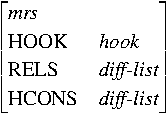
\includegraphics{pdf/mrs-min.pdf}} \\
\evnup{b.} & \evnup{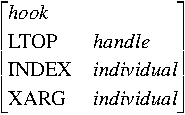
\includegraphics{pdf/hook-min.pdf}} \\ 
\evnup{c.} & \evnup{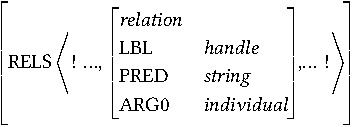
\includegraphics{pdf/rels-min.pdf}} \\
\evnup{d.} & \evnup{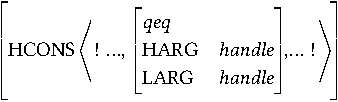
\includegraphics{pdf/hcons-min.pdf}} \\ 
\end{tabular}}}


\noindent First of all, note that AVMs in \myref{avm:mrs-min}, in
which a difference list (i.e.\ \tdl{diff-list}) is used as the value
of RELS and HCONS, are the grammar-internal representations of MRS as
feature structures.\is{MRS}  When MRSs are used as an interface
representation, they use \tdl{list} rather than \tdl{diff-list}, and
do not involve feature structures. Second, HOOK keeps track of the
attributes that need to be externally visible upon semantic
composition, whose minimal components are included in
(\ref{avm:mrs-min}b). The value of LTOP (Local TOP) is the handle of
the relation or relations with the widest fixed scope within the
constituent. The value of INDEX is the index that a word or phrase
combining with this constituent might need access to. The value of ARG
(external ARGument) is identified with the index of a semantic
argument which serves as the subject in raising and control
constructions.\is{raising predicate}\is{control predicate}
Third, REL is a bag of EPs (Elementary Predicates),
whose type is a \tdl{relation}. Each \tdl{relation} has at least three
attributes: LBL (Label), PRED (Predicate), and ARG0 (ARGument
\#0). The value of LBL is a \tdl{handle}, which represents the current
EP. The value of PRED is normally a string, such as
``\_dog\_n\_1\_rel'', ``\_bark\_v\_rel'', etc.\footnote{The PRED value can
  be a type, particularly for incorporating lexical semantics
  (i.e.\ wordnet) into the meaning representation. Besides, even
  though the PRED value is treated as a string, it is structured.}
The value of ARG0 is either \tdl{ref-ind} for EPs introduced by
nominals or \tdl{event-ind} for EPs introduced by verbals, adjectives,
adverbs, and adpositions.\is{adposition}  Depending on the semantic argument
structure of an EP, more ARGs can be introduced. For example,
intransitive verbs (e.g.\ \textit{bark}) additionally have ARG1,
transitive verbs (e.g.\ \textit{chase}) have ARG1 and ARG2, and
ditransitive verbs (e.g.\ \textit{give}) have ARG1, ARG2, and
ARG3. Finally, HCONS represents partial information about scope.  The
value of HCONS is a bag of \tdl{qeq} (equality modulo quantifier)
constraints.


More recently, alternative representations of MRS have been suggested
for ease of utilizing the MRS formalism for a variety of language
applications, which include RMRS (Robust MRS, \citealt{copestake:07}),
and DMRS (Dependency MRS, \citealt{copestake:09}).  RMRS involves the
functionality of \isi{underspecification} of relational information,
which facilitates shallow techniques in language processing (e.g.\ NP
chunking).  DMRS makes use of a dependency style representation
designed to facilitate machine learning algorithms. It mainly aims to
remove redundancies that (R)MRS may have.  The current work makes use
of the conventional version of MRS, but the dependency style
representation DMRS deploys is introduced for ease of explication.



\section{Motivations}
\label{9:sec:motivations}

The use of \isi{ICONS} is motivated by three necessities; (i)
resolving discrepancies between forms and meanings in information
structure, (ii) facilitating underspecifiability in order to allow for
flexible and partial constraints, and (iii) capturing the 
information structure relations between expressions and particular
clauses.  To these, I add a working hypothesis to facilitate (iv)
informative emptiness in representing information structure.



\subsection{Morphosyntactic markings \vs Semantic representation}
\label{9:ssec:ms-vs-sr}

First, the morphosyntactic markings for information structure need to
be kept distinct from semantic markings. This is analogous to the
linguistic fact that morphological tense can sometimes differ from
semantic tense as in counterfactual constructions. Some forms of
expressing information structure do indeed directly indicate specific
information structure roles such as \isi{topic}, \isi{focus}, and
\isi{contrast}. For instance, the contrastive topic marker
\textit{th{\`i}} in \ili{Vietnamese} directly assigns \isi{contrastive
  topic} meaning to the NP that the marker is attached to, as
repeatedly exemplified below.

\myexe{\enumsentence{\label{exe:vie:ch9}
\shortex{4}
  {Nam & th{\`i} & {\textcrd}i & H\`{a} N\textsubdot{\^{o}}i}
  {Nam & \textsc{thi} & go & Ha Noi}
  {`Nam goes to Hanoi(, but nobody else).' [vie] \citep[1]{nguyen:06}}}}

\noindent A specific sentence position can also play the same
role. For example, if the word order is not neutral in \ili{Russian},
the clause-final position assigns the non-contrastive \isi{focus}
meaning,\is{clause-final} while \isi{preposing} is responsible for
\isi{contrastive focus} meaning \citep{neeleman:titov:09}. Yet, quite
a few marking systems do not necessarily reveal which information
structure meanings are being conveyed. The typical case of a
discrepancy between morphosyntactic marking and semantic
representation is the information structure marker \wa in
\ili{Japanese} and \nun in \ili{Korean} as discussed before. Even when
a language has a relatively deterministic relation between forms and
meanings, the correlation is neither perfect nor perfectly
understood. For example, the A-accent in \ili{English} has been widely
evaluated as containing \isi{focus} meaning, but there are some
counterexamples to this generalization as exemplified previously in
Section \ref{4:ssec:conditions} (i.e.\ Second Occurrence Focus). Moreover,
there has been a debate concerning the function of the B-accent, which
could mark (i) just topic \citep{jackendoff:72}, (ii) \isi{contrastive
  topic} \citep{kadmon:01,buring:03}, (iii) theme \citep{steedman:00},
and (iv) \isi{contrast} \citep{hedberg:06}.




\subsection{Underspecification}
\label{9:ssec:underspecification}

Unless there exists a decisive clue to identify the intended
information structure meaning, that meaning is most parsimoniously
represented as underspecified.\is{underspecification}
This proposal is especially crucial for
analyzing sentences which appear in an unmarked word order.  Without
clues to indicate a particular meaning (e.g.\ the \isi{contrastive topic}
marker \textit{th{\`i}} in \ili{Vietnamese}), any constituents in the
unmarked order are not specified for meaning with respect to
information structure. For instance, (\ref{exe:sobaka:ch9}a) presented
again below is in the neutral word order in \ili{Russian}, and the
orthography does not represent prosodic patterns related to
information structure.


\myexe{\eenumsentence{\label{exe:sobaka:ch9}
\item\shortex{2} 
{Sobaka & laet.}
{dog & bark}
{`The dog barks.' [rus]}
\item\shortex{2} 
{Laet & sobaka.}
{bark & dog}
{`The \textsc{dog} barks.' [rus]}}}


\noindent When we do not know which element plays which information
structure role in text-based processing (as in \ref{exe:sobaka:ch9}a),
it would be better to leave the information structure values
underspecified allowing for all meanings that the constituents may
potentially have. On the other hand, with in a sentence like
(\ref{exe:sobaka:ch9}b) we can say the \textit{sobaka} has \isi{focus}
meaning because the subject is not in situ, and the inversion
serves as the clue for determining focus.


As exemplified hitherto, it is not likely that we can precisely
determine an information structure role of each constituent in many
cases, particularly given that sentence-by-sentence processing usually
lacks discourse-related information.  Hence, it is highly necessary to
represent information structure meanings in a flexible way.  For
instance, note the following example in \ili{Greek}.\footnote{The
  subscript in the original example such as []\mysub{C-Foc}, which
  stands for \isi{contrastive focus}, is removed in
  \myref{exe:greek:2} in order to show the difference between the
  neutral sentence and the marked sentence.}


\myexe{\eenumsentence{\label{exe:greek:2}
\item\shortex{2}
{Thelo & kafe.}
{want.1\textsc{sg} & coffee.\textsc{acc}}
{`I would like coffee.'}
\item\shortex{2}
{Kafe & thelo.}
{coffee.\textsc{acc} & want.1\textsc{sg}}
{`Coffee I would like.' [ell] \citep[44]{gryllia:09}}}}


\noindent Because the \isi{postverbal} \isi{focus} \textit{kafe} `coffee' in
(\ref{exe:greek:2}a) takes the object position in the \isi{basic word
  order} and there is no other clue to disclose the information
structure role within the single sentence, it does not have to have
any specific meanings per se. That means that \textit{kafe}
in (\ref{exe:greek:2}a) can be evaluated as containing (i)
\isi{non-contrastive focus}, (ii) \isi{contrastive focus}, or even as being (iii)
\isi{background} if the preceding verb \textit{thelo} `want' plays a
focus role. Hence, the semantic representation of \textit{kafe} in
(\ref{exe:greek:2}a) has to cover all those potential meanings
simultaneously (i.e.\ \tdl{non-topic} in the present study).  On the
other hand, the \isi{preverbal} focus in (\ref{exe:greek:2}b)
(ex situ) presents a clue identifying its information
structure meaning.  In other words, \textit{kafe} in
(\ref{exe:greek:2}b) is constructionally marked and thereby conveys a
more specific meaning than that in (\ref{exe:greek:2}a) and it can no
longer be interpreted as background. Nonetheless, its meaning is still
vague allowing for readings as either non-contrastive focus or
contrastive focus. Thus, the ideal representation would be able to
allow for both meanings while still excluding background as a possible
reading (i.e.\ \tdl{focus} as the supertype of both
\tdl{semantic-focus} and \tdl{contrast-focus}).\is{semantic focus}\is{contrastive focus}


\subsection{Binary relations}
\label{9:ssec:binary}


Third, using \isi{ICONS} is motivated by the necessity of finding
binary relations between a clause and an element used in the
construction of MRSs\is{MRS} that belongs to the clause. These binary
relations are crucial in representing the information structure of
various types of utterances.  The typed feature structure of ICONS
consists of three components to identify which element has which
information structure value within which clause.\is{binary relation}


Information structure roles can be represented not as a property of
the constituent itself, but as a relationship that holds between the
clause and the constituent it belongs to. For example, in the \ili{English}
sentence \textit{The \textsc{dog} barks.}, the subject \textit{the
  \textsc{dog}} with the A-accent should be viewed as the \isi{focus} of
the clause headed by the predicate \textit{barks}, rather than as
simply focused.  This approach is in line with \citet{lambrecht:96}
and \citet{engdahl:vallduvi:96} who regard information structure as a
subtype of sentential grammar.\is{A-accent} That is, whether a
constituent is associated with focus or \isi{topic} should be identified
within the sentence that includes the constituent.


Furthermore, a constituent can have multiple relations with different
clauses. One element can have two (or more) information structure
relations, if it belongs to different clauses simultaneously.  This
notion can be clearly understood if we consider multiclausal
utterances such as those which contain relative and embedded clauses.
Most previous studies on information structure treat only fairly
simple and monoclausal constructions. However, expanding a theory to
include embedded clauses introduces the need to allow a single element
to have multiple information structure meanings.  This is because an
embedded clause not only configures its own information structure, but
also plays an information structure role in the domain of the main
clause that takes the embedded clause as one of the
arguments.\is{relative clause} A typical example of this come from
relative clauses where the antecedent of the relative clauses has
relations with both (i) the verb in the relative clause and (ii) the
other verb in main clause, whose values are not necessarily identical
to each other.



Those kinds of relations have been already captured in an
\isi{LFG}-based study on information structure.\is{relative
  clause}\is{relative pronoun} \citet{bresnan:mchombo:87} argue that
relative pronouns function as the \isi{topic} of relative clauses,
following the theorem presented in \citet{kuno:76}.\footnote{The
  present study does not defer to this
  argument. Section \ref{10:ssec:relative} presents the details.}  In this
analysis, then, relative pronouns are assigned an information
structure value within the relative clause, as shown in
\myref{exe:bresnan:mchombo:87:eng}.


\myexe{\eenumsentence{\toplabel{exe:bresnan:mchombo:87:eng}
\item\evnup{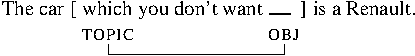
\includegraphics{pdf/bresnan-mchombo-eng-rel.pdf}}
\item\evnup{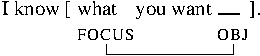
\includegraphics{pdf/bresnan-mchombo-eng-embedded.pdf}}
\item\evnup{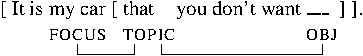
\includegraphics{pdf/bresnan-mchombo-eng-cleft.pdf}} 
\\
\mbox{ } \mbox{ } \mbox{ } \mbox{ } \mbox{ }
\mbox{ } \mbox{ } \mbox{ } \mbox{ } \mbox{ }
\mbox{ } \mbox{ } \mbox{ } \mbox{ } \mbox{ }
\mbox{ } \mbox{ } \mbox{ } \mbox{ } \mbox{ }
\mbox{ } \mbox{ } \mbox{ } \mbox{ } \mbox{ }
  \citep[757--758]{bresnan:mchombo:87}}}


\noindent The antecedent corresponding to the relative pronoun
(e.g.\ \textit{the car} in \ref{exe:bresnan:mchombo:87:eng}a) has an
additional information structure value within the main
clause.\is{relative pronoun}\is{relative clause} Additionally,
embedded constructions realized as free relative clauses
(e.g.\ \textit{what you want} in \ref{exe:bresnan:mchombo:87:eng}b)
play yet another information structure role within the main
clause. The clefted NP (e.g.\ \textit{my car} in
\ref{exe:bresnan:mchombo:87:eng}c) is assigned a \isi{focus}
meaning,\is{clefting} but its relative pronoun (e.g.\ \textit{that} in
\ref{exe:bresnan:mchombo:87:eng}c) plays the \isi{topic} role in the
relative.  While these analyses do not accord perfectly to the
argument presented in the present study, they are still significant
and highlight the necessity of treating information structure as a
relationship between an element and its clause.



\subsection{Informative emptiness}  
\label{9:sec:hypotheses}


In addition to the motivations presented in the previous subsections,
I provide a working hypothesis about informatively empty categories.
\citet[156]{lambrecht:96} argues that expressions which cannot be
stressed, such as expletives (e.g.\ \textit{it} in \textit{It is
  raining.} and \textit{there} in \textit{There is nobody in the
  room.}), unstressed determiners, and so on, cannot be used as \isi{topic}
in principle.  What is to be noted is that they cannot be used for
expressing any other information structure meanings, either.  For this
reason, the present study presents a working hypothesis that
semantically empty categories (e.g.\ complementizers, expletives) and
syncategorematic items\footnote{Syncategorematic items refer to words
  that cannot serve as the main syntactic category of human language
  sentences, such as the subject (in the matrix clause) and the
  predicate.  \citet{lambrecht:96} does not capture any generalization
  about them, but I argue that they cannot be used as topic, either.}
(e.g.\ relative pronouns) are informatively empty as well. This means
no information structure category can be assigned to them, though they
may be required by constructions which serve to mark information
structure, such as the cleft construction in
\ili{English}.\is{clefting}\is{relative pronoun} For example, in
(\ref{exe:void}a), the expletive \textit{it} and the \isi{copula} 
\textit{is} are semantically empty and the relative pronoun \textit{that} is
syncategorematic; thus, they are informatively vacuous. Likewise,
since the copula \textit{was} and the preposition \textit{by} in
\isi{passive} sentences in English are semantically empty, they cannot
take part in information structure in principle, as shown in
(\ref{exe:void}b).\footnote{In colloquial expressions, copular may
  participate in information structure.  For example, if a question is
  given like \textit{Are you a student?}, then the answer can be
  \textit{I \textsc{was} a student.}  In this case, \isi{focus} is assigned
  to a specific linguistic feature, such as \tdl{tense}, rather than a
  specific constituent.  Admittedly, the current model does not handle
  such a peculiar focus assignment.}  \mysout{Strike} in
\myref{exe:void} indicates that they are informatively meaningless.





\myexe{\eenumsentence{\toplabel{exe:void}
\item{{\Midline{It}} {\Midline{is}} the book {\Midline{that}} was torn
  by Kim.}
\item{The book {\Midline{was}} torn {\Midline{by}} Kim.}}}


\noindent Lexical markers to express information structure, such as
case-marking adpositions (e.g.\ nominative \ga in \ili{Japanese}) are
mostly semantically and informatively empty.\is{adposition} Although
they participate in forming information structure and behave as a clue
for identifying information structure meanings, they do not have their
own predicate names, and do not exist in the semantic representation
(i.e.\ MRS as presented here),\is{MRS} either.  In other words, they
assign no information structure values to themselves, but instead
identify and assign information structure values to the phrase that
they are combined with.  Since the information structure constraints
in the representation of the current work are all relative to elements
in the RELS list, what is not represented in the RELS list cannot bear
any information structure value. In sum, semantically empty lexical
items and syncategorematic items are incapable of bearing their own
information structure value, but they can assign an information
structure value to others.



\subsection{Summary}
\label{9:sec:hierarchies}

The motivations and the working hypothesis presented in this section
are rigorously applied within the remaining parts of this
book. They can be summarized as follows.  

\myexe{\eenumsentence{\toplabel{def:mot:hyp}
\item The formal markings of information structure should be
  modeled separately from the semantic representation of information
  structure.
\item The information structure value should be specified so that it
  can cover all potential information structures that a given sentence
  may have.
\item The semantic representation of information structure involves a
  \isi{binary relation} identifying which element has which
  information structure relation to which clause.
\item Semantically empty and syncategorematic items are informatively
  empty.}}


\noindent These hypotheses are built upon in the following chapters
into three type hierarchies: \tdl{info-str}, \tdl{mkg}, and
\tdl{sform}.\is{\textit{info-str}}\is{\textit{mkg}}\is{\textit{sform}}


\section{Information structure \textnormal{(}\tdl{info-str}\textnormal{)}}
\label{9:sec:info-str}



\begin{figure}[!t]
\begin{center} 
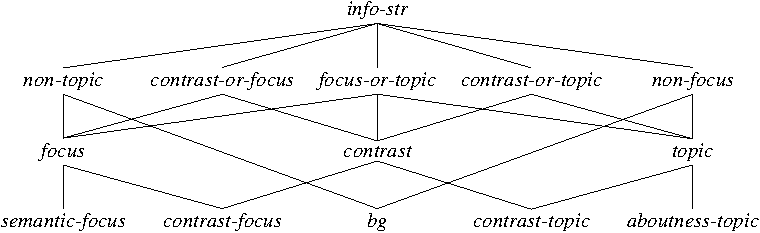
\includegraphics[width=\textwidth]{pdf/info-str.pdf}
\caption{Type hierarchy of \tdl{Info-str}}
\label{fig:info-str}
\end{center}
\end{figure}

\noindent The type hierarchy of \tdl{info-str} is sketched out in
Figure~\ref{fig:info-str}.\is{\textit{info-str}} The values of
information structure are represented as node names (i.e.\ type names)
within the \tdl{info-str} type hierarchy.  For instance, if a
linguistic unit introducing an EP (Elementary Predicate) into RELS is
computed as conveying meaning of \isi{non-contrastive focus}
(i.e.\ \tdl{semantic-focus}), it also introduces one \tdl{info-str}
value whose type name is \tdl{semantic-focus} into ICONS.\is{semantic focus}
The nodes at the bottom represent the most specific meanings, which cannot be
further subdivided with respect to information structure. The nodes in
the third line include the major components of information
structure. \tdl{Focus} and \tdl{topic} are mutually exclusive, and
\tdl{contrast} should be realized with either of them. The nodes in
the second line are abstract. Each of them stands for a linguistic
property that the major components of information structure exhibit:
possibility of topicality or focality (\tdl{non-topic},
\tdl{non-focus}, and \tdl{focus-or-topic}), and possibility of
\isi{contrastiveness} (\tdl{contrast-or-topic} and \tdl{contrast-or-topic}).
These are motivated by the need to capture via
\isi{underspecification} exactly the range of information structure
meanings associated to particular information structure markings in
certain languages, as detailed below.




This \textit{info-str} hierarchy is based on \citet{song:bender:11},
but is extended with several additional nodes. \is{\textit{info-str}}
\tdl{Non-topic} means the target cannot be read as \isi{topic}
(e.g.\ case-marked NPs in \ili{Japanese}).  \tdl{Focus-or-topic} is
assigned to the fronted NPs in focus/topic \isi{fronting} constructions.
\tdl{Contrast-or-topic} is used for \wa in Japanese and \nun in
\ili{Korean}, because \wa or \onun-marked constituents in those
languages can convey a meaning of non-contrastive topic, contrastive
topic, or even contrastive \isi{focus}.  \tdl{Contrast-or-focus} likewise
can be used for forms responsible for a meaning of non-contrastive
focus, contrastive focus, or even contrastive topic.\footnote{Such a
  marking system has not been observed, but it is included into the
  hierarchy as a counterpart of \tdl{contrast-or-topic}.}
\tdl{Non-focus} similarly indicates that the target cannot be the
focus, and would be appropriate for dropped elements in
\textit{pro}-drop languages. As discussed thus far, \tdl{focus} and
\tdl{topic} are mutually exclusive because they designate disjoint
portions of a sentence. \tdl{Focus}, \tdl{contrast}, and \tdl{topic}
multiply inherit from the components in the second row.\is{contrast}\is{focus}
The types in the bottom line represent the fully specified meaning of each
component of information structure.\is{semantic focus} \tdl{Semantic-focus} taken from
\citet{gundel:99} means non-contrastive focus, and
\tdl{aboutness-topic} means non-contrastive \isi{topic}.\is{aboutness topic} Finally, \tdl{bg}
(\isi{background}) means the constituent is neither \tdl{focus} nor
\tdl{topic}, which typically does not involve additional marking but
may be forced by particular positions in a sentence.


Compared to the previous version presented in \citet{song:bender:11}
and other approaches in previous literature, the type hierarchy
illustrated in Figure~\ref{fig:info-str} allows greater
flexibility. First, Figure~\ref{fig:info-str} shows us that
\tdl{contrast}, which is in a sister relation to \tdl{non-topic} and
\tdl{non-focus}, behaves independently of \tdl{topic} and
\tdl{focus}.\is{topic} Second, \tdl{focus-or-topic} and
\tdl{contrast-or-topic} can help in the modeling of the discrepancies
between forms and meanings in information structure (e.g.\ focus/topic
\isi{fronting}, \wa or \onun-marked \isi{focus} in \ili{Japanese} and
\ili{Korean}, etc.), and represent ambiguous meanings involving a
classification across \tdl{focus}, \tdl{topic}, and \tdl{contrast}.
Third, \tdl{non-topic} and \tdl{non-focus} also facilitate more
flexible representation for informatively undetermined items in some
languages. For example, case-marked NPs can convey either focus or
\isi{background} meaning in Japanese \citep{heycock:94}. That is,
since a Japanese case marker (i.e.\ \textit{ga} for nominatives) can
convey two information structure meanings (\tdl{focus} and \tdl{bg}),
the marker itself has to be less specifically represented as
\tdl{non-topic}. Note that \tdl{non-topic} is the supertype of both
\tdl{focus} and \tdl{bg}. Finally, \tdl{bg} is made use of as an
explicit component of information structure.


Using \isi{ICONS} involves several fundamental points in operation as
follows.  First, \isi{ICONS} represents information structure as a
binary relation between two elements. In other words, the current
model regards \tdl{clause} as the locus where information structure is
determined.\footnote{\mbox{[CLAUSE \tdl{individual}]} and
  \mbox{[CLAUSE-KEY \tdl{event}]} at first blush might look like an
  inconsistency.\is{CLAUSE}\is{CLAUSE-KEY} However, \tdl{event} is a
  subtype of \tdl{individual} in the current type hierarchy of the
  \lingo \isi{Grammar Matrix} system. Roughly speaking,
  \tdl{individual} (an immediate subtype of \tdl{index}) is the lowest
  meaningful supertype of \tdl{ref-ind} for nominals and \tdl{event}
  for verbals.}  Second, \isi{ICONS} behaves analogously to HCONS and
RELS in that values of \tdl{info-str} are gathered up from daughters
to mother up the tree. The value type of ICONS, HCONS, and RELS is
\tdl{diff-list}, which incrementally collects linguistic information
during the formation of parse trees.  Additionally, \isi{ICONS} and
HCONS share almost the same format of feature structure. Both are, so
to speak, accumulator lists. The value type in the \tdl{diff-list} of
\isi{ICONS} is \textit{info-str}, and that of HCONS is \textit{qeq},
both of these include two attributes to represent a \isi{binary
  relation} (i.e.\ TARGET to CLAUSE, and HARG to
LARG).\is{CLAUSE}\is{TARGET} Third, despite the similarity in
structure, RELS and HCONS are different from \isi{ICONS} in terms of
how they function in the semantics.  RELS and HCONS directly engage in
the building up of the logical form, and also interact in an intimate
manner with each other. Although \isi{ICONS} also interact with
truth-conditions \citep{partee:91}, this interaction is not
implemented in the same way.  Fourth, HCONS and ICONS also behave
differently in generation. ICONS-based sentence generation is carried
out via a subsumption check, using the type hierarchy whose value type
is \tdl{icons} or its subtypes
(e.g.\ \tdl{info-str}).\is{\textit{info-str}} That is, the generator
first creates all potential sentences that logically fit in the input
MRS without considering the constraints on ICONS,\is{MRS} and then
postprocesses the intermediate results to filter out sentences
mismatching the values on the \isi{ICONS}
list. Chapter~\ref{chapter12} deals with the details of ICONS-based
generation.



\subsection{ICONS}
\label{9:ssec:icons}


\isi{ICONS} is newly added to structures of type \textit{mrs} (i.e.\ under
CONT) as shown in \myref{avm:mrs}.  

\myexe{\enumsentence{\label{avm:mrs}\evnup{
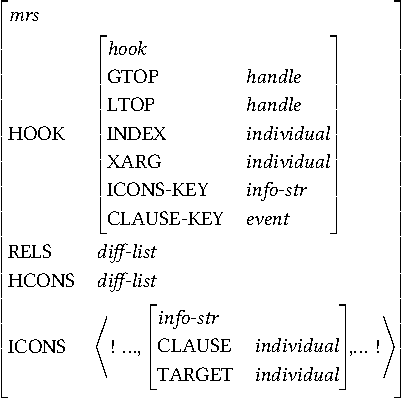
\includegraphics{pdf/icons.pdf}}}}


\noindent An \isi{ICONS} element has two features, namely TARGET and
CLAUSE.\is{CLAUSE}\is{TARGET} When an element is information-structure
marked and also is exhibited as an EP, that element's ARG0 value will
be structure-shared with the value of TARGET.  That is to say, each
type name indicates which information structure meaning is associated
with the EP, and the connection between them is specified by the
co-index between TARGET and ARG0.  On the other hand, the value of
CLAUSE is structure-shared with the INDEX value of the predicate that
functions as the semantic head of the clause.



To take a simple example, (\ref{exe:sample:icons}a) can be represented
as the following AVM (\ref{exe:sample:icons}b).  Note that in
(\ref{exe:sample:icons}a) the subject \textit{\textbf{Kim}} is
B-accented and the object \textit{the \textsc{book}} is
A-accented.\is{A-accent}\is{B-accent}

\myexe{\eenumsentence{\label{exe:sample:icons}
\item{\textbf{Kim} reads the \textsc{book}.}
\item{\evnup{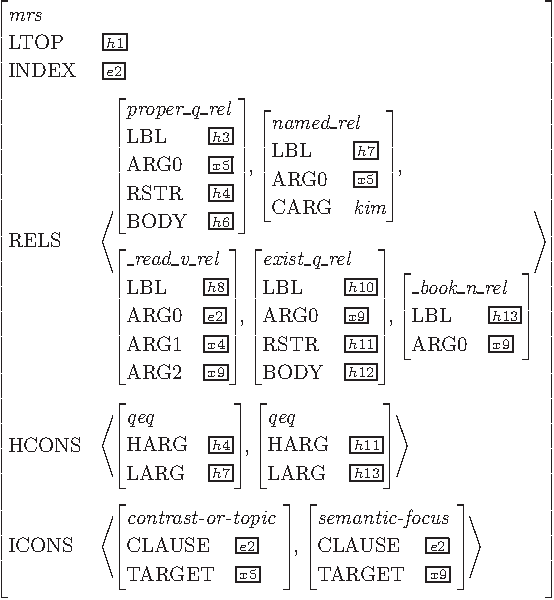
\includegraphics{pdf/sample-mrs.pdf}}}}}


\noindent In (\ref{exe:sample:icons}b), the first element in \isi{ICONS} is
specified as \tdl{contrast-or-topic}, which stands for the information
structure meaning that \textit{\textbf{Kim}} (potentially)
delivers. Likewise, the second element in \isi{ICONS} indicates that
\textit{the \textsc{book}} is evaluated as containing
\tdl{semantic-focus}.\is{semantic focus}  The connection between the elements in ICONS
and the EPs in RELS is determined by the coreference between TARGET of
each \isi{ICONS} element and ARG0 of EP(s). The first element in \isi{ICONS} has
\fbox{\tdl{x5}} for TARGET, and the first and the second EPs in RELS
have the same value. Likewise, the TARGET of the second element in
\isi{ICONS} is co-indexed with the fourth and the fifth EPs' ARG0.\is{CLAUSE} The
values of CLAUSE indicate which EP is the head in the clause. In this
case, the verb \textit{reads} plays the role as indicated by
\fbox{\tdl{e2}}.  The clues to determine information structure
meanings are built up incrementally by lexical and phrasal rules with
an interaction of the type hierarchies. In this case, the rules for
identifying each information structure value are (hypothetical)
lexical rules that constrain the A and B accents.  When a specific
\tdl{info-str} value is created by such a rule, this value is gathered
up to the tree via \tdl{diff-list} \mypage{tdl:diff-list}.


What is key in this method of representation is that the intermediate
types in the hierarchy allow for underspecified representations. As
discussed several times thus far, the grammar of many human languages
does not fully pin down the information structure role an element
plays even when it does provide partial information about it. Because
\tdl{contrast-or-topic} on the first \isi{ICONS} value is not a
terminal node in Figure~\ref{fig:info-str}, \textit{\textbf{Kim}} in
(\ref{exe:sample:icons}a) can be interpreted as any of the categories
subtypes: \tdl{contrast-focus}, \tdl{contrastive-topic},
or \tdl{aboutness-topic}.\is{aboutness topic}\is{contrastive topic}
The specific choice among them can be
determined by the contextual information.  This flexible
representation is crucial in a robust computational model for processing
natural language sentences.








\subsection{ICONS-KEY and CLAUSE-KEY}
\label{9:ssec:icons-key}


In \myref{avm:mrs}, there are two pointers under HOOK; \isi{ICONS-KEY}
and \isi{CLAUSE-KEY}. They are acquired in an incremental way.


ICONS-KEY makes both the phrase/ lexical structure rules and the
lexical entries contribute partial information to the same \isi{ICONS}
element.  When an \tdl{info-str} element can be inserted into the
\isi{ICONS} list, we may not specifically know which information
structure meaning the element carries because information structure
markings often provide only partial information.  The meaning can be
further constrained by multiple sources when the parse tree is further
constructed.  For example, \wa in \ili{Japanese} in itself is assigned
\tdl{contrast-or-topic}, but this meaning can be further constrained
(e.g.\ as \tdl{topic}, \tdl{contrast-topic}, or \tdl{contrast-focus})
by other syntactic operations such as \isi{scrambling}.  Thus, it is
necessary to use a pointer in order to impose a more specific
constraint on an \tdl{info-str} element already augmented in the
\isi{ICONS} list.\is{\textit{info-str}} ICONS-KEY is used for this
purpose.



However, the value of CLAUSE of a constituent cannot be identified
until the clause it belongs to is identified. Thus, when an
\tdl{info-str} element is inserted into the \isi{ICONS} list, the
value of CLAUSE is in most cases not yet specified. This value can be
filled in later by using another pointer called CLAUSE-KEY.  Each
\mbox{ICONS-KEY{$\mid$}CLAUSE} is not lexically bound.\is{CLAUSE} The
value of CLAUSE is naturally identified at the clausal level.  In
other words, the CLAUSE values have to remain unbound until each
clause an individual is overtly expressed in is chosen.\footnote{This
  strategy is different from the approach presented in
  \citet{song:bender:12}, in which \tdl{verbal-lex} and
  \tdl{headed-icons-phrase} take the responsibility of linking
  CLAUSE-KEY to the INDEX of heads. The main reason for the change in
  strategy is that using \tdl{headed-icons-phrase} ends up with
  introducing too many subtypes of
  \tdl{head-comp-phrase}.\is{CLAUSE-KEY} This runs against the spirit
  of the HPSG\is{HPSG} formalism (i.e.\ reducing redundancy and using
  a minimal number of grammatical types).} There are two assumptions
to be noted. The first is that individuals play an information
structure role only with respect to overt clauses.  That is, if an
utterance contains no items that can play a role of the semantic head,
the utterance is assumed to have no CLAUSE binding.\footnote{There are
  some utterances in which no verbal item is used in human language.
  First, if an utterance is vocative (e.g.\ \textit{Madam!}), the
  information structure value of the entire utterance can be evaluated
  as \tdl{focus}.  Second, in languages that do not make use of
  \isi{copula} (e.g.\ \ili{Russian}) copula constructions include
  non-verbal predicates. In this case, since the complement plays the
  semantic head role, the value of CLAUSE is bound to the complement.}
The second is that clauses in this context do not include non-finite
(i.e.\ tenseless) clauses. That is, whether or not a verbal type has a
clausal dependent (subject or complement) is dependent upon whether or
not the dependent involves a verb for which a tense is identified. The
underlined VPs in \myref{exe:PRO} are not clausal arguments. In other
words, the number of clauses in an utterance is the same as the number
of tensed VPs in the utterance.


\myexe{\eenumsentence{\label{exe:PRO}
\item Kim seems \underline{to sleep}.
\item Kim tried \underline{to sleep}.
\item Kim saw Fido \underline{sleeping}.
\item Kim made Fido \underline{sleep}.
\item Kim promised Lee \underline{to leave}. 
\item Kim believed Lee \underline{to have left}.}}


The framework of the \lingo \isi{Grammar Matrix} employs a type hierarchy
representing clausal types, as sketched out in \myref{fig:clause}. The
\tdl{clause} hierarchy is already implemented in the core of the
\lingo Grammar Matrix system (i.e.\ \texttt{matrix.tdl}).


\myexe{\enumsentence{\label{fig:clause}\evnup{
      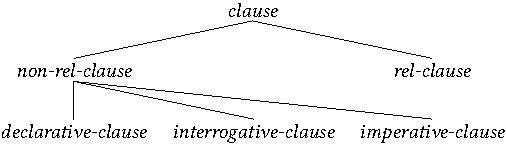
\includegraphics{pdf/clause.pdf}}}}



\noindent Among the nodes in \myref{fig:clause}, \tdl{non-rel-clause}
and \tdl{rel-clause} are responsible for constraining the CLAUSE
values.  The CLAUSE values of the elements on the \isi{ICONS} list
become co-indexed with the INDEX of the semantic head of the CLAUSE
(i.e.\ the value of INDEX being structure-shared with the value of
ARG0 of some EP whose label is the value of LTOP).  This constraint on
\tdl{non-rel-clause} is represented in \myref{avm:non-rel-cl}, in
which CLAUSE-KEY is identified with its INDEX.
 
\myexe{\enumsentence{\label{avm:non-rel-cl}\evnup{
      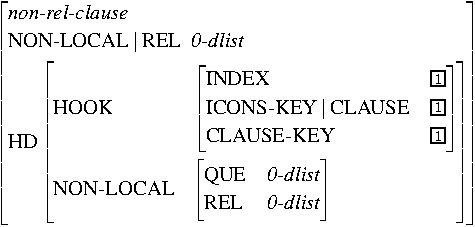
\includegraphics{pdf/non-rel-clause.pdf}}}}

\noindent Because every element in a single clause shares the same
CLAUSE-KEY,\is{CLAUSE-KEY} this coreference is also applied to all
information structure values' \mbox{ICONS{$\mid$}CLAUSE} in
ICONS.\footnote{The constraint on
  \tdl{non-rel-clause} shown in \myref{avm:non-rel-cl} would be incompatible
  with some interrogative sentences in \ili{Bulgarian}:
  \tdl{0-list} in NON-LOCAL{$\mid$}QUE can cause a problem in
  that Bulgarian employs multiple \isi{\textit{wh}-fronting}
  \citep{grewendorf:01}.  Nonetheless, the constraint on
  \tdl{non-rel-clause} is presented as is, because the current
  proposal focuses on information structure in the \lingo \isi{Grammar
    Matrix}. The \isi{\textit{wh}-fronting} is beyond the scope of the
  present work, but should be addressed in future work.} For instance,
lexical types that have an intransitive argument structure (e.g.\ an
intransitive verb \textit{bark} in \ili{English}) inherit from the type
depicted in AVM \myref{avm:intransitive}.  The CLAUSE-KEY of the
subject is identified with the verb's CLAUSE, but the specific value
is not yet given.\is{CLAUSE}\is{CLAUSE-KEY}



\myexe{\enumsentence{\label{avm:intransitive}\evnup{
        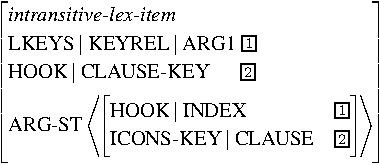
\includegraphics{pdf/intransitive-lex-item.pdf}}}}

\noindent The CLAUSE values (not yet specified) of the elements on the
\isi{ICONS} list are specified when a clause is constructed by
\myref{avm:non-rel-cl}.\is{ICONS-KEY} The same goes for adjuncts in a
single clause.  Adjuncts (e.g.\ attributive adjectives, adverbs, etc.)
and the heads they are modifying share the same value of
CLAUSE.\is{CLAUSE}\is{CLAUSE-KEY} That is, the ICONS-KEY{$\mid$}CLAUSE
and CLAUSE-KEY of NON-HEAD-DTR is identified with the CLAUSE value of
ICONS-KEY of HEAD-DTR. More information about this is given in
Section \ref{10:sec:monoclausal}
\mypage{avm:head-mod-phrase}.





In \texttt{matrix.tdl} in the \lingo \isi{Grammar Matrix} system, the
subtypes of \tdl{head-subj-phrase} also inherit from the types at the
bottom in \myref{fig:clause} (e.g.\ \tdl{declarative-clause},
etc.). Hence, the instance types (e.g.\ \tdl{decl-head-subj-phrase}
and \tdl{decl-head-opt-subj-phrase}) naturally bear the constraint
\myref{avm:non-rel-cl}.\is{CLAUSE-KEY} In other words, instances of
\tdl{head-subj-phrase} are responsible for the binding of CLAUSE-KEY.




\subsection{Summary}
\label{9:ssec:icons-summary}

As discussed thus far, in order to see the larger picture of how
information is packaged in an utterance, it is necessary to look at
(i) which element has (ii) which information structure relation to
(iii) which clause. In particular, if an utterance is made up of two
or more clauses, a single entity can have an information structure
relation (e.g\ \isi{topic}, \isi{focus}, and so on) with each clause, and those
relations are not necessarily the
same.\is{\textit{info-str}}\is{binary relation} Leveraging binary
relations meets this need specifically TARGET for (i), CLAUSE for
(iii),\is{CLAUSE}\is{TARGET} and a value of \tdl{info-str} (i.e.\ a
node in the type hierarchy) for (ii). The items on the ICONS list are
feature structures of type \textit{info-str}, which indicate which
index (the value of TARGET) has a property of information structure
and with respect to which clause (the value of CLAUSE).  Information
structure meanings conveyed by each individual are represented in MRS
as an element of the \isi{ICONS} list,\is{MRS} which our
\isi{infrastructure} of machine translation can refer to for both
transfer and generation.\is{transfer-based}\is{generation}



\section{Markings \textnormal{(}\tdl{mkg}\textnormal{)}}
\label{9:ssec:mkg}

The information structure marking itself is recorded via a
morphosyntactic feature MKG (MarKinG)\is{MKG}\is{\textit{mkg}} inside
of \mbox{SYNSEM{$\mid$}CAT}, which places lexical and syntactic
constraints on forms expressing information structure meanings.  MKG
features are exclusively concerned with markings of information
structure. They are particularly of use for constraining the
\isi{scrambling} constructions in \ili{Korean} and \ili{Japanese},
which will be deeply analyzed in Section \ref{10:sec:scrambling}
  \mypage{10:sec:scrambling}. Before delving into those details, the
  present subsection presents the basic functionality of the feature
  structure.


MKG plays two roles in handling information structure; one is
theoretically driven, and the other is practical.  First, MKG
contributes to resolving discrepancies between form and meaning in
information structure. As mentioned earlier, the MKG value reflects
the morphosyntactic marking, but does not necessarily coincide with
the semantic value.  For instance, \wa in \ili{Japanese} and \nun in
\ili{Korean} (as discussed in Section \ref{5:sec:lex}) can sometimes convey a
contrastive \isi{focus} reading as exemplified in \myref{exe:kor:cf:ch9}:
\textit{ecey-nun} `yesterday-\textsc{nun}' in the answer should be
evaluated as conveying a meaning of contrastive focus.  In this case,
the value of MKG that \textit{ecey-nun} has (under CAT) is \tdl{tp},
but the information structure value in semantic representation is
\tdl{contrast-focus}.


\myexe{\eenumsentence{\label{exe:kor:cf:ch9}
\item[Q:]\shortex{3}
{Kim-i& onul & o-ass-ni?}
{Kim-\textsc{nom} &	today & come-\textsc{pst}-\textsc{int}}
{`Did Kim come today?'}
\item[A:]\shortex{4}
{ani. & (Kim-un) & ecey-nun & o-ass-e.}
{No. &	Kim-\textsc{nun} & yesterday-\textsc{nun} & come-\textsc{pst}-\textsc{decl}}
{`No. Kim came yesterday.' [kor]}}}

\noindent Second, MKG also functions as a flag feature for blocking
overgeneration.  The typical instantiation that might be overgenerated
but for MKG is \tdl{topic-comment} constructions, which the next
subsection elaborates on.\is{topic-comment}


The type \tdl{mkg} is used as the value of the feature MKG, and
introduces two further features, FC (FoCus-marked) and TP
(ToPic-marked).\is{\textit{mkg}}


\begin{figure}[!t]
\begin{center} 
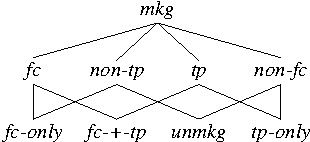
\includegraphics{pdf/hmkg.pdf}
\caption{Type hierarchy of \tdl{Mkg}}
\label{fig:mkg}
\end{center}
\end{figure}


\myexe{\enumsentence{\label{avm:mkg}\evnup{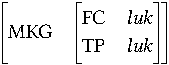
\includegraphics{pdf/mkg.pdf}}}}

\noindent The value type of TP and FC is \tdl{luk}, which is a
supertype of \tdl{bool} (boolean) and \tdl{na} (not-applicable).  As
shown in \myref{avm:mkg}, \tdl{luk} consists of six subtypes including
+, --, and \tdl{na}, and can therefore capture the marking type of
constituents more flexibly than \tdl{bool} which, as shown below, only
has subtypes for + or --.


\myexe{\enumsentence{\label{fig:luk}\evnup{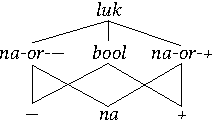
\includegraphics{pdf/luk.pdf}}}}


\noindent The value of MKG\is{MKG} is always a subtype of \tdl{mkg},
as sketched out in Figure~\ref{fig:mkg},\is{\textit{mkg}} in which
\tdl{tp} is constrained as \mbox{[TP +]}, \tdl{non-tp} as
\mbox{[TP \tdl{na-or-${-}$}]}, \tdl{fc} as \mbox{[FC +]}, and
\tdl{non-fc} as \mbox{[FC \tdl{na-or-${-}$}]}. Types at the bottom
multiply inherit from the intermediate supertypes, and thereby both FC
and TP are fully specified.  Instantiations of the \tdl{mkg} values
assigned to particular information structure markings are as follows.


Focus and topic markers in some languages have a fairly
straightforward MKG value. For instance, the contrastive \isi{topic} marker
in \ili{Vietnamese} \textit{th{\`i}} presented in \myref{exe:vie:ch9}
is \mbox{[MKG \tdl{tp-only}]}.  The focus clitics \textit{{\'e}} and
\textit{{\'a}} in \ili{Rendile} exemplified in \mypage{exe:rel} are
\mbox{[MKG \tdl{fc-only}]}. The clitic \textit{=m} in Ingush conveys a
contrastive \isi{focus} meaning \mypage{exe:inh:contrast}, which also
involves \mbox{[MKG \tdl{fc-only}]}. The two types of Cantonese
particles \mypage{exe:man:part}, such as \textit{aa4} for topic and
\textit{aa3} for focus, are \mbox{[MKG \tdl{tp-only}]} and \mbox{[MKG
    \tdl{fc-only}]}, respectively.


The A and B accents in \ili{English}, in line with the analysis in
\citet{hedberg:06}, are also straightforwardly assigned. The A-accent
(H*) is responsible for conveying a non-contrastive \isi{focus} meaning,
whereas the B-accent (L+H*) can be used to express topic (irrespective
of contrastive or non-contrastive) or contrastive focus.\is{B-accent}
\is{A-accent}\is{B-accent} The A-accent exclusively used for marking
focus is \mbox{[MKG \tdl{fc-only}]}, while the B-accent can be left
underspecified with a value like \mbox{[MKG \tdl{tp}]}.




Lexical markers in \ili{Japanese} and \ili{Korean} only partially
constrain meaning. As is well known, Japanese and Korean employ three
types of NP markings; (i) case-marking (e.g.\ \ga and \ika for
nominatives), (ii) \wa and \onun-marking, and (iii) null-marking
(expressed as \ensuremath{\emptyset}~in the examples presented thus far).\is{lexical
  markers} The distinction among their MKG values is crucially used in
handling the interaction between lexical markings and \isi{scrambling}
in these languages (discussed in detail in Section \ref{10:sec:scrambling}).
Initially, the case markers are \mbox{[MKG \tdl{unmkg}]},\is{MKG}
given that they are not expressly markers of information structure,
although they indirectly influence information structure meanings
(i.e.\ \tdl{non-topic}, \citealt{heycock:94}). Yet, \tdl{unmkg} does
not necessarily imply a case-marked constituent cannot be used for
\isi{focus} or \isi{topic}. Note that, in the current analysis,
information structure markings are neither a necessary condition nor a
sufficient condition for information structure meanings.  Second, the
MKG value of \wa and \nun may be either \tdl{tp} or a fully specified
type such as \tdl{tp-only}. The present study supports the former,
because contrastively used markers and non-contrastively used ones show
different prosodic behavior from each other in \ili{Korean} and
\ili{Japanese} \citep{chang:02,nakanishi:07}.  For example, as already
provided in Chapter~\ref{chapter8} \mypage{avm:chang:tf},
\citet{chang:02} argues that non-contrastive (`thematic' in his
terminology) \isi{topic} has \mbox{[STR \ensuremath{<1>}]} while
contrastive topic has \mbox{[STR \ensuremath{<3>}]} in
Korean.\is{non-contrastive topic} If we can deploy a resolution system
distinguishing the difference between them in the future, the value of
\mbox{MKG{$\mid$}FC} would not remain underspecified, and thereby the
information structure will be more concretely
constrained.\is{underspecification} In other words, non-contrastively
topic-marked constituents will have \mbox{[MKG \tdl{tp-only}]},
whereas contrastively topic-marked ones will have \mbox{[MKG
    \tdl{fc-+-tp}]}. \tdl{Fc-+-tp} as shown in Figure~\ref{fig:mkg}
means both values of MKG{$\mid$}FC and MKG{$\mid$}TP are +. Note that
these values do not violate the theorem that \isi{focus} and topic are
mutually exclusive.  Since MKG is exclusively concerned with markings,
\tdl{fc-+-tp} does not imply the constituent is regarded as containing
both focus and \isi{topic}.  This value indicates that the constituent
is either focused-marked or topic-marked.  \mbox{[MKG{$\mid$}TP +]}
will come from the lexical information of \nun, and
\mbox{[MKG{$\mid$}FC +]} will be obtained from the prosodic
information of the constituent (i.e.\ \mbox{[STR
    \ensuremath{<3>}]}).\is{prosody} However, a completely reliable
system for detecting prosody in Japanese and Korean, to my knowledge,
is non-existent for now.  The value of MKG{$\mid$}FC of the topic
markers, therefore should (and does) remain underspecified in the
current work.  Finally, null-marked phrases in Japanese and Korean
should be evaluated as remaining undetermined with respect to
information structure markings
(i.e.\ \tdl{unmkg}).\is{underspecification}




The MKG feature also plays a role in calculating the extent of
\isi{focus projection}.\is{prosody} As surveyed in the previous
chapter, most previous HPSG-based analyses of information structure
assume that prosody expressing \isi{focus} is responsible for
spreading the meaning of focus to larger constituents
\citep{bildhauer:07}.  However, focus is projected onto larger phrases
not only by means of prosody but also by lexical markers in some cases
\citep{choe:02}.\is{lexical markers} The feature responsible for
\isi{focus projection} in the current proposal is \mbox{[MKG{$\mid$}FC
    +]}.\footnote{The A-accent in \ili{English} and the prosodic
  pattern of marking focus in \ili{Spanish} inherently have
  \mbox{[MKG{$\mid$}FC +]}, which originally comes from
  \mbox{[UT{$\mid$}DTE +]}, if we include the phonological structure
  and related rules suggested by \citet{bildhauer:07} into the
  grammars.\is{A-accent}\is{MKG}}




\section{Sentential forms \textnormal{(}\tdl{sform}\textnormal{)}}
\label{9:ssec:sform}


The value of \isi{ICONS} can be constrained by phrasal types as well
as lexical types.\is{sentential forms}\is{\textit{sform}} In order to
capture a generalization about syntactic combination between two
phrases with respect to information structure, a type hierarchy
representing sentential forms is required. Recall that many previous
studies argue that information structure contributes to a sentential
grammar
\citep{lambrecht:96,engdahl:vallduvi:96,paggio:09,song:bender:11}.
Building on the previous literature, I propose Figure~\ref{fig:sform}
as the classification of phrasal types. The main purpose of
\tdl{sform} is to arrange information structure components in a
sentence.\is{sentential forms} However, this type hierarchy is not
concerned with the linear ordering of components, unlike
Figure~\ref{fig:hier:paggio} given in the previous
chapter \mypage{fig:hier:paggio}.\is{sentential forms}



\begin{figure}[!t]
\begin{center} 
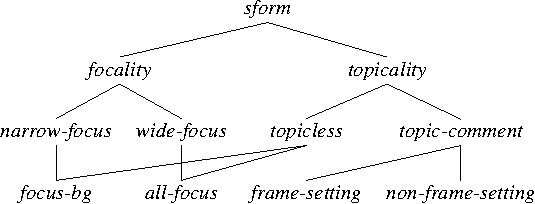
\includegraphics{pdf/sform.pdf}
\caption{Type hierarchy of \tdl{Sform}}
\label{fig:sform}
\end{center}
\end{figure}


\citet{lambrecht:96} posits that information structure is deeply
associated with how a sentence is formed. \citet{engdahl:vallduvi:96},
likewise, regard information structure (information packaging in their
terminology) as a part of sentential grammar. \citet{paggio:09}
provides a hierarchy for representing sentential forms in Danish as
shown in Figure~\ref{fig:hier:paggio},\is{sentential forms} which is
quite similar to Figure~\ref{fig:sform}. \citeauthor{paggio:09}'s type
hierarchy terminates in various phrasal rules that simultaneously
inherit from other fundamental phrasal rules. This method is also
taken up by \citet{song:bender:11}.  In \citeauthor{song:bender:11}'s
analysis of \isi{scrambling} in \ili{Japanese} and \ili{Korean}
(i.e.\ in the OSV order), the combination of scrambled objects and VPs
forms an instance whose type inherits from both \tdl{head-comp-phrase}
and \tdl{topic-comment}.\is{topic-comment} The current model follows the same
combinatoric strategy for placing constraints on phrase structure
types with respect to information structure.


However, there is a methodological difference between what was
proposed in previous literature and that in the present study. In
previous studies the types representing sentential forms also
characterize the linear order of components. For instance, the
instruction-types provided in \citet{engdahl:vallduvi:96}, such as
\tdl{link-focus}, \tdl{link-focus-tail}, \tdl{all-focus}, and
\tdl{focus-tail}, and the node names in the hierarchies of
\citet{paggio:09} and \citet{song:bender:11}, such as
\tdl{topic-focus} and \tdl{topic-bg-focus}, reflect constraints on the
ordering of elements.  In Figure~\ref{fig:sform},\is{sentential forms}
by contrast, only \tdl{topic-comment} is constructed based on linear
order.\is{topic-comment} All the other types merely represent the components that the
construction comprises without respect to the linear
order. \tdl{Focus-bg} in Figure~\ref{fig:sform}, which is normally
used for clefts constructions,\is{clefting} does not mean that
\tdl{focus} is necessarily followed by \tdl{bg}.  For example, focused
constituents are postposed in the cleft constructions in \ili{Korean}
\citep{kim:yang:09}, but these constructions are nonetheless instances
of \tdl{focus-bg}.  In the current work, the linear order of the
components is manipulated by phrase structure rules in each language
grammar.




The types of \tdl{sform} interact with MKG features to stratify
meaning of information structure at the phrase
level.\is{\textit{sform}} The \tdl{sform} types are inherited by
phrase structure rules. Not all phrase structure rules inherit from
\tdl{sform} types, but if a specific syntactic operation is used for
expressing information structure (e.g.\ \isi{scrambling} in
\ili{Japanese} and \ili{Korean}), the rule for the constructions
inherits from something in Figure~\ref{fig:sform}.



Since sentential forms are basically a matter of how two phrases are
combined with each other,\is{sentential forms} \tdl{sform} inherits
from \tdl{binary-headed-phrase} (made up of HEAD-DTR and
NON-HEAD-DTR). We may ask why it is necessary to refer to MKG features
of daughters in building up parse trees and why \tdl{sform} is
required to be additionally introduced as a single phrase structure
type.  Several types of constructions use \tdl{sform}.  Those include
(i) the \isi{preverbal}/\isi{postverbal} position of focused
constituents, (ii) cleft constructions,\is{clefting} (iii) comment
markers (e.g.\ \textit{sh\`{i}} in Mandarin \ili{Chinese} and
\textit{ba} in \ili{Abma}) that always entail \isi{focus projection},
and (iv) \isi{scrambling} in \ili{Japanese} and \ili{Korean}
\citep{choi:99,ishihara:01,song:bender:11}. These are respectively
relevant to (i) \tdl{narrow-focus}, (ii) \tdl{focus-bg}, (iii)
\tdl{wide-focus}, and (iv) \tdl{topicless} \vs
\tdl{topic-comment}.\is{narrow focus}\is{wide
  focus}\is{topic-comment}\is{topicless}




\tdl{Sform} is bipartitely divided into \tdl{focality} and
\tdl{topicality}, which indicates marking (i.e.\ values of MKG) and/or
meaning (i.e.\ values of ICONS) of components of information structure
in the arguments.\is{\textit{mkg}}\is{\textit{sform}} \tdl{Sform} and
its subtypes, as presented below, place constraints on MKG,\is{MKG}
which implies sentences are realized depending on information
structure markings of elements.  Since \tdl{sform} also places
constraints on ICONS, it serves to relate the marking to the meaning.


\tdl{Focality} takes \tdl{fc-only} as the value of MKG, which
indicates the phrase includes a \isi{focus}-marked constituent.
\tdl{Focality} is divided into \tdl{narrow-focus} and
\tdl{wide-focus}.\is{narrow focus}\is{wide focus} The distinction
between them, however, is not necessarily equivalent to argument focus
\vs predicate focus \citep{lambrecht:96,erteschik:07}, because verbs
can bear \tdl{narrow-focus}.  As shown in \myref{avm:focality}, only
the MKG value on the mother is restricted in \tdl{focality}. The value
is used for further composition: Some phrase structure rules prevent
focus-marked constituents (i.e.\ specified as \mbox{[MKG{$\mid$}FC
    +]}) from being used as the daughter. Some phrase structure rules,
on the contrary, require an explicitly focus-marked constituent as the
daughter.


\myexe{\enumsentence{\label{avm:focality}\evnup{
      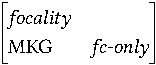
\includegraphics{pdf/focality.pdf}}}}


\tdl{Topicality} is mainly concerned with how the \isi{topic} is realized in
a sentence. \tdl{Topicality} does not have any specific constraint for
now, because \tdl{topicless} and \tdl{topic-comment} are unlikely to
share a feature cross-linguistically.\is{topic-comment}\is{topicless}
Nonetheless, it is introduced
into the hierarchy out of consideration for symmetry with
\tdl{focality}.  Subtypes of \tdl{topicality} are constrained in the
following way.


\myexe{\enumsentence{\toplabel{avm:topicless:topic-comment}
\begin{tabular}[t]{lllll}
a. & \evnup{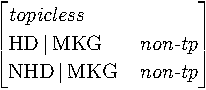
\includegraphics{pdf/topicless.pdf}} & &
b. & \evnup{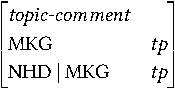
\includegraphics{pdf/topic-comment.pdf}} \\
\end{tabular}}}


\noindent Note that \tdl{topic-comment} has a constraint on the MKG
value of the mother, just as \tdl{focality} above has the constraint
\mbox{[MKG \tdl{fc-only}]}.  In \tdl{topic-comment} constructions
(e.g.\ \textit{as for ...}  constructions),\is{topic-comment} topics are followed by
other constituents. Once a construction is identified as
\tdl{topic-comment}, there are two options in further composition. If
there exists another \isi{topic} in the left side, and the topic is a
\isi{frame-setter}, then further composition is allowed. Otherwise,
the \tdl{topic-comment} instance itself cannot be used as a head
(i.e.\ a secondary \tdl{comment}) in further composition.\is{topic-comment}  The
subtypes of \tdl{topic-comment} (i.e.\ \tdl{frame-setting} and
\tdl{non-frame-setting}) details this
distinction.\is{topic-comment}\is{frame-setting}


As noted, not all sentences have topics.\is{clefting}\is{topicless}
Cleft constructions are presumably \tdl{topicless} in many
languages.\footnote{There exists some exception to this
  generalization. It is reported that some languages
  (e.g. \ili{Spanish}) allow for left-dislocated topics in cleft
  constructions.} Accordingly, a constituent with \mbox{[MKG{$\mid$}TP
    +]} cannot be the non-head-daughter in cleft constructions. For
example, cleft clauses in \ili{Korean} show a strong tendency to be
exclusive to \onun-marked constituents, as exemplified below.


\myexe{\eenumsentence{\label{exe:clefts:kor:ch9}
\item\shortex{5}
  {ku & chayk-ul/*un & ilk-nun & salam-i/un & Kim-i-ta.}
  {the & book-\textsc{acc}/\textsc{nun} & read-\textsc{rel} & person-\textsc{nom}/\textsc{nun}  & Kim-\textsc{cop}-\textsc{decl}}
  {`It is Kim that reads the book.'}
\item\shortex{5}
  {Kim-i/*un & ilk-nun & kes-i/un & ku & chayk-i-ta.}
  {Kim-\textsc{nom}/\textsc{nun} & read-\textsc{rel} & thing-\textsc{nom}/\textsc{nun} & the & book-\textsc{cop}-\textsc{decl}}
  {`It is the book that Kim reads.' [kor]}}}


The distinction between \tdl{topicless} and \tdl{topic-comment} is
especially significant in topic-prominent languages, such as
\ili{Chinese}, \ili{Japanese}, and \ili{Korean}, in which forms of
marking topics play an important role in syntactic configuration
\citep{li:thompson:76,huang:84}.\is{syntactic positioning}
\citet{lambrecht:96} regards \myref{exe:kuroda}, in which \textit{inu}
`dog' is combined with the nominative marker \ga instead of the
so-called \isi{topic} marker \wa, as a topicless
sentence.\footnote{\citet{kuroda:72} regards \myref{exe:kuroda} as a
  subjectless sentence.}  This is further evidence that not all
subjects are topics.\is{topicless}


\myexe{\enumsentence{\label{exe:kuroda}
\shortex{3}
{inu ga & hasitte iru.}
{dog \textsc{nom} & running}
{`The dog is running.' [jpn]  \citep[161]{kuroda:72}}}}


\noindent In line with \citeauthor{lambrecht:96}'s claim, the present
analysis provides for this with the type \tdl{topicless}.  The
difference between \tdl{topicless} and \tdl{topic-comment} performs a
role in constructing \ili{Japanese} and \ili{Korean} grammars, which
is partially proposed in \citet{song:bender:11}.\is{topic-comment} For instance,
\tdl{head-subj-rule} and \tdl{head-comp-rule} in these languages need
to be divided into several subrules, depending on whether the
non-head-daughter of the rules are \wa or \onun-marked or not.  The
rules dependent upon the value of MKG in Japanese and Korean are
provided in Section \ref{10:sec:scrambling}.




There is a need to refine the meaning of \tdl{topicless}.\is{topicless}
On one hand, it indicates that \isi{topic} is not realized in surface form, not that
there is no topic at all in the utterance.  For example,
\tdl{topicless} in \ili{Japanese} means that the non-head-daughter of
the phrase is not \wa-marked.  For example, since \textit{inu ga} `dog
\textsc{nom}' in \myref{exe:kuroda} is not a \wa-marked constituent,
and it constitutes the sentence with the predicate \textit{hasitte
  iru} `running' as a non-head-daughter, the sentence ends up being
\tdl{topicless}.\is{MKG} On the other hand, MKG only reflects overtly
expressed items and an utterance might have an implicit topic which is
not overtly expressed as is the case in \isi{topic-drop}, which often occurs
in topic-prominent languages (e.g., \ili{Chinese}, \ili{Japanese}, \ili{Korean}).
It is true that dropped topics in the current work surely
have a representation in the ICONS, but they are irrelevant to MKG.



\tdl{Narrow-focus} and \tdl{focus-bg} come under \tdl{focality}, but
constraints on them are language-specific.\is{narrow focus} This is
because they are not reflected in the linearization of components. For
example, assume two hypothetical languages Language \textit{A} and
\textit{B}, which have a symmetrical property as
follows.\footnote{Language \textit{A} is hypothetically modeled quite
  analogously to Hungarian \citep{kiss:98,szendroi:99}. Hungarian is
  known as adopting SVO word order preferentially
  \citep{gell:ruhlen:11}, though it is sometimes reported that the
  word order in Hungarian is pragmatically conditioned (i.e.\ no
  dominant order, \citealt{kiefer:67}).}
 

\myexe{\eenumsentence{\label{def:lang-a}
\item Language \textit{A} employs SVO as its \isi{basic word order}.
\item Focused constituents in Language \textit{A} are realized in the immediate
  preverbal position.
\item Additionally, there is an optionally used accent, which
  expresses focus.}}


\myexe{\eenumsentence{\label{def:lang-b}
\item Language \textit{B} employs SOV as its \isi{basic word order}.
\item Focused constituents in Language \textit{B}~ are realized in the
  immediate \isi{postverbal} position.
\item The same as (\ref{def:lang-a}c)}}


\noindent Based on (\ref{def:lang-a}-\ref{def:lang-b}), the object in
SOV word order in Language \textit{A} and the objects in SVO word
order in Language \textit{B} are narrowly focused.\is{narrow focus}
They participate in \tdl{narrow-focus} as a non-head-daughter. Both
[OV] in Language \textit{A} and [VO] in Language \textit{B} are
instantiated as \tdl{head-comp-phrase}, but the former is constrained
by \tdl{head-final} in which the head (i.e.\ the verb) follows its
complement, while the latter is constrained by \tdl{head-initial} in
which the head precedes. Thus, from a cross-linguistic perspective,
linear order does not have to be used as a key to constrain
\tdl{narrow-focus}.\is{narrow focus} On the other hand, a distinction
between HEAD-DTR and NON-HEAD-DTR cannot be used for constraining
\tdl{narrow-focus}, either.  For instance, focused constituents in
clefts behave as the head of cleft clauses realized as
relatives.\is{clefting} In other words, while the focused items in
[OV/VO] in Language \textit{A} and \textit{B} respectively are
NON-HEAD-DTRs, the focused items in cleft are HEAD-DTRs. In
a nutshell, it is true that \tdl{narrow-focus} and \tdl{focus-bg}
require some constraints on information structure marking and meaning,
but the constraints must be applied on a language by language or
construction by construction basis.


There are at least two subtypes of \tdl{focus-bg} across languages:
One where the HD involves [MKG \tdl{fc}] and one where the NHD does.
For example, the cleft constructions (as an instance of
\tdl{focus-bg}) in \ili{English} basically inherit the following
AVM. More specific constraints can be imposed
language-specifically.\is{clefting}

\myexe{\enumsentence{\label{avm:focus-bg}\evnup{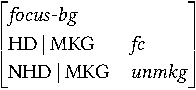
\includegraphics{pdf/focus-bg.pdf}}}}

\noindent This AVM serves to prevent constituents with information
structure markers from being used in cleft constructions. For
instance, \nun in \ili{Korean} is not allowed to be used in cleft
clauses, as exemplified in \myref{exe:kor:cleft:apple:7}.\is{clefting}


\myexe{\enumsentence{\label{exe:kor:cleft:apple:7}
\shortex{4}
  {Kim-i/*un & mek-nun & kes-un & sakwa-i-ta.}
  {Kim-\textsc{nom}/\textsc{nun} & eat-\textsc{rel} & thing-\textsc{nun} & apple-\textsc{cop}-\textsc{decl}}
  {`It is an apple that Kim is eating.' [kor]}}}

\noindent If a grammar employs a set of phrase structure rules that
transmit the MKG value of the subject in the cleft clause to the
higher phrase node, then only the nominative marker that involves [MKG
  \tdl{unmkg}] can be chosen.  The [MKG \tdl{tp}] feature \nun
involves prevents the clause from being used in the clefted clause (see
Section \ref{9:ssec:jpn:kor}).


To present another instance, \tdl{narrow-focus} in Language \textit{A}
can be constrained as follows. Note that the values on HD and NHD are
the reverse of those in \myref{avm:focus-bg}.\is{narrow focus}

\myexe{\enumsentence{\label{avm:narrow-focus}\evnup{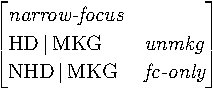
\includegraphics{pdf/narrow-focus.pdf}}}}

\noindent \myref{avm:narrow-focus} also explains the ungrammaticality
of pseudo sentence (\ref{exe:lang-a}c) in Language \textit{A}; HD of
\tdl{narrow-focus} requires a minus value as a value of MKG{$\mid$}FC,
which conflicts with a \isi{focus} accent that falls on the verb. Because
presumably there is no other way to construct (\ref{exe:lang-a}c), a
pseudo sentence like (\ref{exe:lang-a}c) remains ungrammatical.

\myexe{\eenumsentence{\label{exe:lang-a}
\item subj verb obj. (in the neutral word order)
\item subj obj verb. (focus on obj)
\item *subj obj \textsc{verb}. (a focus-marking accent on verb)}}


\noindent A sample derivation for (\ref{exe:lang-a}b) can be sketched
out as \myref{fig:lang-a}, showing only information
structure markings and sentential forms. Note that MKG is seen only
locally, because it is not a head feature. Thus, the value would not
be transmitted to the higher nodes if it were not for an extra
constraint.


\myexe{\enumsentence{\label{fig:lang-a}\evnup{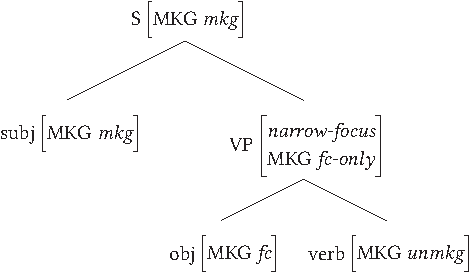
\includegraphics{pdf/lang-a.pdf}}}}


\tdl{Wide-focus},\is{wide focus} next, is particularly related to realization of
comment markers as mentioned earlier. For instance, Mandarin
\ili{Chinese} employs \textit{sh\`{i}} as exemplified below, which
indicates the remaining part after it is in the \isi{focus} domain
\citep{prince:12}.\footnote{\citet{prince:12} says this
  \textit{sh\`{i}} is different from the \isi{copula} \textit{sh\`{i}}
  (i.e.\ homonym).} In a similar vein, \citet{li:09} regards
\textit{sh\`{i}} as a marker responsible for contrastive meanings: The
constituents after \textit{sh\`{i}} are contrastively focused.\is{contrast}


\myexe{\enumsentence{\label{exe:shi:1}
\shortex{4} 
{Zh\={a}ngs\={a}n & [sh\`{i} & [xu\'{e}x\'{i} & y\={\i}xu\'{e}]].}
{Zhangsan & \textsc{shi} & study & medicine}
{`Zhangsan studies medicine.' [cmn] \citep[336]{prince:12}}}}


\noindent Thus, the type of construction licensed by \textit{sh\`{i}}
(and comment markers in other languages such as \ili{Abma},
\citealt{schneider:09}) has to inherit \myref{avm:wide-focus}.  Note
that this constraint is language-universal, unlike
\tdl{narrow-focus}.\is{narrow focus} In the context of \isi{grammar
  engineering} for the \lingo \isi{Grammar Matrix} system,
\myref{avm:wide-focus} is encoded into \texttt{matrix.tdl}, while the
AVM for \tdl{narrow-focus} could be either empty or encoded in
\texttt{mylang.tdl}.  In accordance with \myref{avm:wide-focus}, any
constituents after the comment marker should not be topic-marked.

\myexe{\enumsentence{\label{avm:wide-focus}\evnup{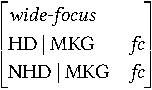
\includegraphics{pdf/wide-focus.pdf}}}}



\tdl{All-focus} inherits from both \tdl{wide-focus} and
\tdl{topicless}.\footnote{Regarding the status of \tdl{all-focus},
  \citet[232]{lambrecht:96} argues that there is a clear
  difference from other types of focused constructions in that the
  pragmatic core of \tdl{all-focus} is ``an absence of the relevant
  presuppositions''.  The argument sounds convincing, but the present
  study does not represent such pragmatic information on the AVMs of
  \tdl{sform}.\is{sentential forms}\is{\textit{sform}}} Finally, it is
necessary to discriminate between \tdl{frame-setting} and
\tdl{non-frame-setting}.\is{topicless} As noted, this use of the MKG feature aims to
pass up appropriate values; in particular, when a topic-marked
constituent occurs in the leftmost
position. \mbox{[NHD{$\mid$}L-PERIPH +]} in (\ref{avm:frame-setting}a)
imposes this constraint.\is{frame-setting}\is{periphery}
\isi{L-PERIPH} (Left-PERIPHeral) will be discussed in the next chapter
(Section \ref{9:ssec:periphery}).



\myexe{\eenumsentence{\toplabel{avm:frame-setting}
\item\evnup{\includegraphics{pdf/frame-setting.pdf}}
\item\evnup{\includegraphics{pdf/non-frame-setting.pdf}}}}


\noindent As seen in Chapter~\ref{chapter3}
(Section \ref{3:sssec:multiple-topics}) topics that function to restrict the
frame of what the speaker is speaking about (i.e.\ so-called
\isi{frame-setting} topics) can appear multiply.\is{topic}

In \ili{English}, while left-dislocated NPs cannot occur more than
once without affecting grammaticality as shown in
(\ref{exe:multiple-topic:eng:2}a),\footnote{This generalization is
  language-specific, not universal.  Some counterexamples have been
  reported: \citet[123]{vallduvi:93} argues for \ili{Catalan} that
  ``There is no structural restriction on the number of phrases that
  may be right or left detached.''  Left-dislocated NPs in
  \ili{Spanish} are also sometimes multiply used
  \citep[224]{zagona:02}.}  frame-setters such as
\textit{yesterday} in (\ref{exe:multiple-topic:eng:2}b) can occur
multiple times in the sentence-initial position as presented in
(\ref{exe:multiple-topic:eng:2}d).\is{frame-setter} In other words,
\tdl{topic-comment} constructions can be used as another comment, and
do not constrain the value of MKG of the head-daughter.\is{topic-comment}
However, they cannot be used again for \tdl{non-frame-setting}.

 
\myexe{\eenumsentence{\label{exe:multiple-topic:eng:2}
\item{*Kim, the book, he read it.}
\item{Yesterday, Kim read the book.}
\item{The book, Kim read it.}
\item{Yesterday, the book, Kim read it.}}}



To sum up,\is{sentential forms} \tdl{sform} is concerned with
syntactic combination between two phrases with respect to information
structure.  This places constraints on both MKG and ICONS, relating
the marking to the meaning. In other words, \tdl{sform} makes
information structure marking and meaning interact with each other.
The type hierarchy here used is adapted from the proposal of
\citet{paggio:09}. The current proposal has one method in common with
\citeauthor{paggio:09}'s: If a phrase structure rule is related to
expressing information structure, it can multiply inherit from both a
specific type of \tdl{sform} and an ordinary phrase structure type,
such as \tdl{head-subj-phrase}, \tdl{head-comp-phrase}, etc. The main
difference between \citeauthor{paggio:09}'s approach and mine is that
my \tdl{sform} hierarchy does not directly constrain the linear order
of components.\is{\textit{sform}}



\section{Graphical representation}
\label{9:sec:graph}


\citet{song:bender:12} suggest representing constraints on information
structure in the style of the dependency graphs of DMRS (Dependency
MRS; \citealt{copestake:09}) for ease of exposition.\is{MRS} Likewise,
the remainder of this book makes use of dependency graphs to present
information structure relations between individuals and clauses.

In these graphs, the \isi{ICONS} values are represented as links
between informatively contentful elements (introducing the referential
index as the value of TARGET) and verbs (introducing the event
variable as the value of CLAUSE) and as unary properties of verbs
themselves.\is{CLAUSE}\is{TARGET} The direction of a given arrow
stands for the \isi{binary relation} between a TARGET (an entity) and
a CLAUSE that the TARGET belongs to.  The start point indicates the
constituent that occupies the CLAUSE-KEY within the clause.  The end
point refers to the constituent whose INDEX is shared with the TARGET,
and whose ICONS-KEY{$\mid$}CLAUSE is co-indexed with the
CLAUSE-KEY.\is{ICONS-KEY} The node name on each arrow indicates the
information structure value that the binary relation has, such as
\tdl{focus}, \tdl{topic}, and so forth.\is{focus}\is{topic}

For example, a dependency graph (\ref{fig:sample:graph}b), which
stands for the binary relations on the ICONS list, is a shorthand
version of the corresponding MRS representation
(\ref{fig:sample:graph}a), which stands for \textit{\textbf{Kim} reads
  the \textsc{book}}. in which the B-accented \textit{\textbf{Kim}}
conveys meaning of contrast and/or topic,\is{B-accent} and the
A-accented \textit{\textsc{book}} bears non-contrastive
\isi{focus}.\is{A-accent}\is{B-accent}\is{contrast}


\myexe{\eenumsentence{\label{fig:sample:graph}
\item\evnup{\includegraphics{pdf/sample-mrs.pdf}}
\item\evnup{\includegraphics{pdf/sample-graph.pdf}}}}


\noindent The arc from \textit{reads} to \textbf{Kim} means that the
index of \textbf{Kim} has a \tdl{contrast-or-topic} relation to the
clause represented by \textsc{reads}.\footnote{The present
  study, according to the argument of \citet{hedberg:06}, regards the
  A-accent (i.e.\ marked as \textsc{small caps}) as prosodic means
  expressing \isi{non-contrastive focus} (i.e.\ \tdl{semantic-focus}),\is{semantic focus}
  and  the B-accent (i.e.\ \textbf{boldfaced}) as conveying one of the
  meanings of \isi{non-contrastive topic}, \isi{contrastive topic}, or sometimes
  \isi{contrastive focus}.} The arc from \textit{reads} to \textsc{book},
likewise, means the index of \textsc{book} has a \tdl{semantic-focus}
relation to the index of \textsc{reads}.\is{semantic focus} The root arrow on
\textsc{reads} indicates that the verb is linguistically
underspecified with respect to the clause that it heads.



\section{Summary}
\label{9:sec:summary}

This chapter has outlined three considerations motivating the
representation of information structure via ICONS: resolving
discrepancies between forms and meanings in information structure,
facilitating underspecifiability for allowing flexible and partial
constraints,\is{underspecification} and capturing the fact that
information structure relations are between expressions and particular
clauses.  Additionally, the ICONS-based representation reflects the
working hypothesis that semantically empty and syncategorematic items
are informatively empty.  Guided by these considerations, I provide
three type hierarchies: \tdl{info-str} whose value types stratify
information structure meaning, \tdl{mkg} indicating morphosyntactic
markings of information structure,\is{MKG}\is{\textit{mkg}} and
\tdl{sform} that works with MKG relating to the \tdl{info-str}
value.\is{sentential forms}\is{\textit{sform}} \isi{ICONS} is added
into \tdl{mrs}, and the value is a \tdl{diff-list} of \tdl{info-str}.
\isi{ICONS} identifies which element has which information structure
relation to which clause. For this purpose, the typed feature
structure of \tdl{info-str} includes TARGET and
CLAUSE.\is{CLAUSE}\is{TARGET} TARGET is identified with the EP's INDEX
(i.e.\ \tdl{individual}), and CLAUSE is determined by the subtype(s)
of \tdl{clause}.\is{ICONS-KEY} In addition, ICONS-KEY and CLAUSE-KEY
are used as pointers during the construction of parse trees.  MKG has
two features; one is FC (FoCus-marked), and the other is TP
(ToPic-marked). These features are independent of meanings represented
as an \tdl{info-str} type.  The next chapter will discuss how these
elements are used to impose constraints on information structure and
represent it in MRS.\is{MRS}
























\chapter{Individual Constraints: Specifics of the Implementation}
\label{chapter10}
\setcounter{enums}{0}


This chapter dives into the details of implementing ICONS (Individual
CONStraints)\is{individual constraints} into MRS (Minimal Recursion
Semantics (\citealt{copestake:etal:05}),\is{MRS} or Meaning
Representation System in the current context) by constraining lexical
types and phrasal types. \myS{10:sec:lexical} shows how information
structure is dealt with in various lexical types.
\myS{10:sec:monoclausal} gives an explanation of information structure
constraints on phrasal types. Next, \myS{9:sec:other-constraints}
presents three additional constraints for configuring information
structure in a specific way.  Building upon the hierarchies and
constraints presented thus far, \myS{9:sec:samples} illustrates how
information structure is represented via \isi{ICONS} in four languages
(\ili{English}, \ili{Japanese}, \ili{Korean}, and \ili{Russian}).


\section{Lexical Types}
\label{10:sec:lexical}


This section largely addresses which lexical item inherits from which
\tdl{icons-lex-item} type out of \tdl{no-icons-lex-item},
\tdl{basic-icons-lex-item}, \tdl{one-icons-lex-item}, and
\tdl{two-icons-lex-item}. They are constrained as presented in the
following AVMs.


\myexe{\enumsentence{\label{avm:icons-lex-item}
\begin{tabular}[t]{lllll}
\evnup{a.} & \evnup{\includegraphics{pdf/no-icons-lex-item.pdf}} & & \evnup{b.} &
\evnup{\includegraphics{pdf/basic-icons-lex-item.pdf}} \\ \evnup{c.} &
\evnup{\includegraphics{pdf/one-icons-lex-item.pdf}} & & \evnup{d.} &
\evnup{\includegraphics{pdf/two-icons-lex-item.pdf}} \\
\end{tabular}}}


\noindent The first two AVMs do not inherently have an \tdl{info-str}
element on the \isi{ICONS} list,\is{\textit{info-str}} but
information-structure related rules can insert a value into the list
for the second type.  That is, if there is a clue for identifying its
information structure value, a value of \tdl{info-str} is introduced
into the the list of \isi{ICONS} and its TARGET is co-indexed with the
HOOK{$\mid$}INDEX of the word.  The last two inherently have non-empty
\isi{ICONS} lists. That means that they lexically have an
\tdl{info-str} value in ICONS.\is{\textit{info-str}}



Lexical entries that cannot be marked with respect to information
structure inherit from \tdl{no-icons-lex-item}
(\ref{avm:icons-lex-item}a). In other words, information structure
markings are not-applicable to them, a constraint formalized as [MKG
  [FC \tdl{na}, TP \tdl{na}]].\is{MKG}\is{relative pronoun} For
example, relative pronouns and expletives in \ili{English} are
instances of \tdl{no-icons-lex-item}.  Other contentful items
introducing an EP inherit from one of the types in
(\ref{avm:icons-lex-item}b-d). The choice among them depends on how
many clauses are subcategorized by the lexical type.  The prefixes
represent how many clauses are created by the type: \tdl{Basic-} means
the lexical type does not include any clausal subject or clausal
complement in ARG-ST. \tdl{One-} means either a clausal subject or a
clausal complement is subordinate to the lexical type. \tdl{Two-}
means there exists a clausal subject and also a clausal complement.
If a verbal type forms a monoclausal construction, the
\tdl{icons-lex-item} type of that verbal item is the basic one
(i.e.\ \tdl{basic-icons-lex-item}).  If a verbal type has ARG-ST
information that includes one or more clausal argument(s)
(i.e.\ multiclausal), its \tdl{icons-lex-item} type is either
\tdl{one-icons-lex-item} (a sentential complement or a sentential
subject) or \tdl{two-icons-lex-item} (both of them).  The extra
\tdl{info-str} values in (\ref{avm:icons-lex-item}c-d) are required
for this purpose.



\subsection{Nominal Items}
\label{10:ssec:nominal}

Nominal items, including common nouns, proper nouns, and pronouns,
inherit from \tdl{basic-icons-lex-item}.  One exceptional lexical type
is that of expletives (e.g.\ \textit{it} in \ili{English}), because
they cannot be marked with respect to information structure
\citep{lambrecht:96}.  Expletives inherit from
\tdl{no-icons-lex-item}.  One question regarding \tdl{info-str} of
nominal items is whether different types of nominals can participate
in information structure in the same way and with the same status. The
current work does not recognize any difference in the information
structure of nominal items.  In other words, other than
\tdl{basic-icons-lex-item}, there is no further information structure
constraint on nominal items.


Pronouns have been regarded as a component associated with information
structure in a different way \citep{lambrecht:96}.  Pronouns, roughly
speaking, can be divided into two categories (i) unaccented and (ii)
accented. \citeauthor{lambrecht:96} argues that the distinction
between these two categories can be sufficiently explained in terms of
information structure.  Across languages, (i) unaccented pronouns
preferentially involve topics.  This finding is bolstered by the
evidence that unaccented pronouns are the most frequently used form of
expressing \isi{topic} in Spoken \ili{French} \citep{lambrecht:86}.
Besides, unaccented pronouns cannot be used for expressing
\isi{focus}, because they are incompatible with
\myref{def:buring:10:ch10-1}.\is{focus prominence}

\myexe{\enumsentence{\label{def:buring:10:ch10-1} Focus Prominence:
    Focus needs to be maximally
    prominent. \citep[p.\ 277]{buring:10}}}

\noindent On the other hand, (ii) accented pronouns can be divided
again into (ii-a) those with a \isi{topic}-marking accent, and (ii-b)
those with a focus-marking accent. \citeauthor{lambrecht:96}
illustrates the linguistic distinction between (ii-a) and (ii-b) in
Italian as follows.

\myexe{\eenumsentence{\label{exe:lambrecht:pro:ita}
\item\shortex{2}
{\textsc{Io} & \textsc{pago}.}
{I & pay.}
{`\textsc{I}'ll pay.' [ita]}
\item\shortex{2}
{Pago & \textsc{io}.}
{pay & I}
{`\textsc{I}'ll pay.' [ita] \citep[p.\ 115]{lambrecht:96}}}}


\noindent The preverbal pronoun \textit{\textsc{Io}} in
(\ref{exe:lambrecht:pro:ita}a) expresses a \isi{topic}, with a rising
intonation contour. On the other hand, the pronoun conveying a
\isi{focus} meaning in (\ref{exe:lambrecht:pro:ita}b) occurs
sentence-finally, and has a falling intonation contour, indicating the
end of the assertion.


From a theoretical point of view, it seems clear that pronouns show
different behaviors in packaging information.\footnote{The nominal
  items also differ from each other in discourse status.
  \citet{kaiser:09} argues that the use of different kinds of
  referring expressions is relevant to the salience of the
  antecedents; the more salient antecedent it refers to, the more
  reduced a form (e.g.  dropped subjects) appears.  That is, selecting
  a type of referential form largely hinges on how salient the
  antecedent is.  The discourse status of nominal categories that take
  \tdl{ref-ind} (a subtype of \tdl{individual}) as the value type of
  HOOK{$\mid$}INDEX is represented as COG-ST (COGnitive-STatus) in the
  current \lingo \isi{Grammar Matrix} system \citep{bender:goss:08}.
  Discourse status is related to information status (e.g.\ given
  \vs. new); COG-ST covers information status from a higher
  level. Information status, as discussed in Chapter~\ref{chapter3},
  has often been studied in tandem with information structure, but it
  is neither a necessary nor a sufficient condition for information
  structure.  In sum, since discourse status is not directly
  responsible for representing information structure, the current work
  leaves discourse-related information to future work.} However, the
current work, based on text processing, cannot deploy such a
division. Phenomena related to (ii) can be modeled with hypothetical
suffixes such as `-a' and `-b', however the responsibility is borne by
the hypothetical suffixes or alternatively lexical rules introducing
the prosodic information, not the pronouns themselves.





\subsection{Verbal Items}
\label{10:ssec:verbal}


The analysis proposed here uses the event variable associated with the
head of the clause to stand in for the clause, and as a result, the
lexical types for verbs (typical clausal heads) need to be constrained
appropriately.  Most contentful verbal items inherit from either
\tdl{basic-icons-lex-item}, \tdl{one-icons-lex-item}, or
\tdl{two-icons-lex-item}.  Verbs inherently have lexical information
about how many elements exist on the \isi{ICONS} list and how they are
bound with the semantic head in the clause that the elements belong
to. That means the number of elements on the \isi{ICONS} list depends
on how many clausal dependents a verbal type has.  This information is
specified inside the ARG-ST of verbal types.  If a verb takes no
clausal phrase(s) as its dependent(s), the verb locally constitutes a
monoclausal phrase. In this case, no element is required to be
included on the \isi{ICONS} list (i.e.\ \tdl{basic-icons-lex-item}).
In some cases, a verb lexically places an information structure
constraint on its subordinated clause(s).  If the ARG-ST of a verbal
type includes either one clausal subject or one clausal complement,
the verbal type constitutes a locally embedded constructions in which
one clause is subordinate to the main clause
(i.e.\ \tdl{one-icons-lex-item}). Sometimes, both the subject and one
of the complements can be clausal. In this case, two elements of
\tdl{info-str} are needed on the \isi{ICONS} list
(i.e.\ \tdl{two-icons-lex-item}).



There is an exception: Some semantically and informatively empty
verbal items are not able to be marked with respect to information
structure. These verbs inherit from \tdl{no-icons-lex-item}. For
example, semantically empty copulae (e.g.\ specificational copulae
\ili{English}) are incapable of contributing an \isi{ICONS}
element.\is{copula}



\subsubsection{Main Verbs}
\label{10:sssec:main-verbs}

Because main verbs in principle can be marked with respect to
information structure, they do not inherit from
\tdl{no-icons-lex-item}. Excluding \tdl{no-icons-lex-item} for this
reason, main verbs can be one of these three types of
\tdl{icons-lex-item}: \tdl{basic-icons-lex-item},
\tdl{one-icons-lex-item}, or \tdl{two-icons-lex-item}.


Common verbs that constitute a monocalusal construction
(e.g.\ intransitives (e.g.\ \textit{bark} in
(\ref{fig:verbal:common}a), transitives (e.g.\ \textit{read} in
(\ref{fig:verbal:common}b), and ditransitives (e.g.\ \textit{give} in
(\ref{fig:verbal:common}c)), inherit from
\tdl{basic-icons-lex-item}. Causative verbs (e.g.\ \textit{make} in
(\ref{fig:verbal:common}d)) and perception verbs (e.g.\ \textit{see}
in (\ref{fig:verbal:common}e)) also inherit from
\tdl{basic-icons-lex-item}, because their verbal complements, such as
\textit{bark} in (\ref{fig:verbal:common}d) and \textit{barking} in
(\ref{fig:verbal:common}e), are tenseless (i.e.\ infinite).  Thus, all
dependents, including the subject and the complements, are bound to
the verb that functions as the semantic head in the sentence (i.e.\ an
element that takes the INDEX in the finite clause).\is{CLAUSE} That
means the CLAUSEs of the dependents are co-indexed with the
HOOK{$\mid$}INDEX of the main verb by
\tdl{non-rel-clause} \mypage{avm:non-rel-cl} which
\tdl{decl-head-subj-phrase} inherits from.  Note that some relations
of information structure are not captured in the following
graphs. This is because if there is no specific clue to identify the
information structure meaning a constituent conveys, no value is
gathered into the list of ICONS. For ease of exposition, in the
following examples, the left-most elements (i.e.\ subjects) are
B-accented (conveying \tdl{contrast-or-topic}) and the right-most
elements are A-accented (conveying
\tdl{semantic-focus}).\is{A-accent}\is{B-accent}\is{semantic focus}


\myexe{\enumsentence{\toplabel{fig:verbal:common}
\begin{tabular}[t]{llllllll}
a. & \evnup{\includegraphics{pdf/the-dog-barks_g.pdf}} & & b. &
\evnup{\includegraphics{pdf/kim-reads-the-book.pdf}} \\ c. &
\evnup{\includegraphics{pdf/kim-gives-lee-the-book.pdf}} & & d. &
\evnup{\includegraphics{pdf/kim-makes-the-dog-bark.pdf}} \\ e. &
\evnup{\includegraphics{pdf/kim-sees-the-dog-barking.pdf}} \\
\end{tabular}}}


Raising and control verbs have the same mapping type in
\tdl{info-str}; every dependent marked with respect to information
structure within a single clause has a co-index between its CLAUSE and
the INDEX of the semantic head in the clause (i.e.\ matrix clause
verb).\is{raising predicate}\is{control predicate}\is{CLAUSE}



\myexe{\eenumsentence{\toplabel{fig:verbal:rasing:control} 
\item \evnup{\includegraphics{pdf/kim-seems-to-read-the-book2.pdf}}
\item \evnup{\includegraphics{pdf/kim-seems-to-read-the-book.pdf}}
\item \evnup{\includegraphics{pdf/kim-tries-to-read-the-book2.pdf}}
\item \evnup{\includegraphics{pdf/kim-tries-to-read-the-book.pdf}}}}


\noindent For example, \textit{the \textsc{book}} in
(\ref{fig:verbal:rasing:control}b) is syntactically a complement of
\textit{read}, but is informatively bound to \textit{seems} whose
INDEX is connected to the INDEX in the clause.  Additionally, it is
interesting that \textit{Kim} has an \tdl{info-str} role in the matrix
finite clause,\is{\textit{info-str}} even though it is not the
semantic argument of \textit{seems}. The same goes for a control verb
\textit{try} in (\ref{fig:verbal:rasing:control}c-d).\footnote{As is
  well-known, raising verbs (e.g.\ \textit{seem}, \textit{appear},
  \textit{happen}, \textit{believe}, \textit{expect}, etc.) and
  control verbs (e.g.\ \textit{try}, \textit{hope}, \textit{persuade},
  \textit{promise}, etc.) display several different properties, such
  as the semantic role of the subject, expletive subjects,
  subcategorization, selectional restriction, and meaning preservation
  \citep{kim:sells:08}. Nonetheless, they have
  \tdl{basic-icons-lex-item} in common as their supertypes, because
  they do not take tensed clauses as complements.}




Several verbal types take clausal complements as shown in
(\ref{fig:verbal:embedded}a) or clausal subjects as shown in
(\ref{fig:verbal:embedded}b), and these inherit from
\tdl{one-icons-lex-item}.

\myexe{\enumsentence{\toplabel{fig:verbal:embedded} 
\begin{tabular}[t]{ll}
a. & \evnup{\includegraphics{pdf/kim-thinks-fido-chases-the-dog.pdf}} \\
b. & \evnup{\includegraphics{pdf/that-the-dog-barks-surprises-kim.pdf}} \\
\end{tabular}}}




\noindent In (\ref{fig:verbal:embedded}a), the arrow from
\textit{chases} and \textit{dog} is locally established within the
embedded clause.  The \isi{binary relation} in the embedded clause
does not have to do with the main verb \textit{thinks}. The main verb
\textit{thinks} also has an arrow to the subject \textit{Kim} in the
local domain. The key point of this example is the arrow from the main
verb \textit{thinks} to the verb in the embedded clause
\textit{chases}. This arrow is introduced by element on the ICONS list
of \tdl{think} (\tdl{one-icons-lex-item}), and shows which information
structure relation the embedded clause has to the matrix
clause. Likewise, the arrow from \textit{surprises} and
\textit{chases} in (\ref{fig:verbal:embedded}b) represents the
inherent \tdl{info-str} element on the \isi{ICONS} list of
\textit{surprise}.


Both subjects and complements can be clausal at the same time.  In
these cases, it is necessary to inherit from \tdl{two-icons-lex-item}.
A typical example can be found in pseudo-clefts,\is{clefting}
including \textit{wh}-clefts, and inverted \textit{wh}-clefts as
exemplified in \myref{exe:verbal:triple}.\footnote{
  \myref{exe:verbal:triple} is originally taken from the ICE-GB
  (\citealt{nelson:etal:02}), and the expressions in angled brackets
  represent the indices of each sentence in the corpus.}  In
\myref{exe:verbal:triple}, the matrix verb \textit{is} inherently has
two elements of \tdl{info-str} on the \isi{ICONS}
list:\is{\textit{info-str}} The CLAUSE value of the first element is
its INDEX, and the TARGET is co-indexed with the INDEX of the verb in
the clausal subject (i.e.\ \textit{happened}). The CLAUSE of the
second is still linked to its INDEX, and the TARGET is co-indexed with
the INDEX of the verb in the complement
(i.e.\ \textit{caught}).\is{CLAUSE}




\myexe{\enumsentence{\label{exe:verbal:triple}
[What happened] is [they caught her without a
  license]. \ensuremath{<}S1A-078 \#30:2:A\ensuremath{>}}}




\noindent The dependency graph corresponding to
(\ref{exe:verbal:triple}) is presented in
\myref{fig:verbal:triple}. Note that the second arrow in
(\ref{exe:verbal:triple}) is specified as \tdl{focus}. That is, the
clausal complement in a \textit{wh}-cleft (e.g.\ \textit{they caught
  her without a license} in \myref{exe:verbal:triple}) is focused
\citep{kim:07}.\is{clefting} Since the other constituents cannot be
assigned \isi{focus}, the clausal subject in (\ref{exe:verbal:triple}) is
specified as \tdl{non-focus}. The verbal entry \textit{is} includes
these values as lexical information.


\myexe{\enumsentence{\toplabel{fig:verbal:triple} 
\begin{tabular}[t]{ll}
\evnup{\includegraphics{pdf/wh-cleft1.pdf}}  \\
\end{tabular}}}





\subsubsection{Adjectives}
\label{10:sssec:adjectives}


Predicative adjective items are the same as the verbal items presented
thus far. The copula \textit{is} in \myref{exe:verbal:adj} is assumed
to be semantically and informatively empty, with the adjective
functioning as the semantic head of such sentences. This constraint is
specified in the following AVM, which passes up the CLAUSE-KEY of the
second argument (i.e.\ the adjective).\is{copula}

\myexe{\enumsentence{\label{avm:copula-verb-lex}
  \evnup{\includegraphics{pdf/copula-verb-lex.pdf}}}}


\noindent \textit{Happy} in (\ref{exe:verbal:adj}a) and \textit{fond
  of} in (\ref{exe:verbal:adj}b), which do not
constitute multiclausal constructions, inherit from
\tdl{basic-icons-lex-item}. Next, \textit{obvious} in
(\ref{exe:verbal:adj}c-d) takes clausal subjects, and \textit{sure}
and \textit{curious} in (\ref{exe:verbal:adj}e-f) take clausal
complements. These inherit from \tdl{one-icons-lex-item}.



\myexe{\eenumsentence{\label{exe:verbal:adj}
\item Kim is happy.
\item Kim is fond of apples.
\item That the dog barks is obvious.
\item It is obvious that the dog barks.
\item Kim is sure that the dog barks.
\item Kim is curious whether the dog barks.}}


\noindent There are also raising adjectives (e.g.\ \textit{likely})
and control adjectives (e.g.\ \textit{eager}), which, like raising and
control verbs, inherit from \tdl{basic-icons-lex-item}.\is{raising
  predicate}\is{control predicate}



Attributive adjectives are different in that they do not introduce the
\tdl{info-str} value that take their own event variable as the value
of CLAUSE.  Attributive adjectives and the nouns they are modifying
share the value of CLAUSE,\is{CLAUSE} which is co-indexed with the
INDEX of the verb heading the clause that they are part of.  For
example, the arrows on \textit{big} in \myref{fig:verbal:ajd} come
from the main verb of each sentence.  This linking strategy is
constructionally constrained by
\tdl{head-mod-phrase}. \myS{10:sec:monoclausal} gives an explanation
of how this linking is achieved via \tdl{head-mod-phrase}.






\myexe{\enumsentence{\toplabel{fig:verbal:ajd}
\begin{tabular}[t]{llllllll}
a. & \evnup{\includegraphics{pdf/the-big-dog-barks-1.pdf}} & &
b. & \evnup{\includegraphics{pdf/kim-reads-the-big-book.pdf}} \\
\end{tabular}}}




There is a distinction between attributive and predicative adjectives
with respect to building up the list of ICONS, but there is no need to
use an extra lexical rule to discriminate them. What is of importance
is incrementally gathering \tdl{info-str} values into the list of
ICONS,\is{\textit{info-str}} and this strategy is achieved by phrase
structure rules, such as \tdl{head-comp-rule} for predicative
adjectives (as specified in the ARG-ST of \myref{avm:copula-verb-lex})
and \tdl{head-mod-rule} for attribute ones (see
\myref{avm:head-mod-phrase} presented in the next section).



\subsubsection{Auxiliaries}
\label{10:ssssec:auxiliaries}





As far as \isi{ICONS} is concerned, auxiliaries in \ili{English} are divided
into two subtypes.\is{auxiliary} One contributes no predicate and no
\isi{ICONS} element, and thereby inherits from
\tdl{no-icons-lex-item}.  The other introduces an EP to RELS, and
thereby inherits from \tdl{basic-icons-lex-item}. Since complements of
auxiliaries are always non-finite, there are no auxiliaries of type
\tdl{one-icons-lex-item} or \tdl{two-icons-lex-item}.\is{auxiliary} An
example of the first category, \tdl{will} in (\ref{fig:verbal:aux}a)
is semantically empty, and does not occupy the INDEX of the
clause. Such an auxiliary, therefore, does not have any \tdl{info-str}
element in ICONS, either. Instead, the main verb, \textit{read} in
(\ref{fig:verbal:aux}a), has arrows to each of its dependents. By
contrast, \textit{can} in (\ref{fig:verbal:aux}b) introduces an EP to
RELS and has arrows to all individuals that introduce \tdl{info-str}
into the clause.\footnote{Its LKEYS{$\mid$}KEYREL{$\mid$}PRED is
  specified as `\_can\_v\_modal\_rel' in the ERG.}


\myexe{\enumsentence{\toplabel{fig:verbal:aux}
\begin{tabular}[t]{llllllll}
a. & \evnup{\includegraphics{pdf/kim-will-read-the-book.pdf}} & &
b. & \evnup{\includegraphics{pdf/kim-can-read-the-book.pdf}} \\
\end{tabular}}}

\noindent As stated above, these two types of auxiliaries inherit from
different lexical types.\is{auxiliary} \textit{Will} is an instance of
\tdl{no-icons-lex-item}, and therefore does not participate in the
articulation of information structure. Second, \textit{can} inherits
from the the type given in
\myref{avm:trans-first-arg-raising-lex-item-1}. The CLAUSE value of
the subject (i.e.\ the first element in ARG-ST) is co-linked to its
own CLAUSE-KEY,\is{CLAUSE}\is{CLAUSE-KEY} and the second argument
(i.e.\ the VP) also shares the CLAUSE value with its own
CLAUSE-KEY.\footnote{Note that
  \myref{avm:trans-first-arg-raising-lex-item-1} actually contains
  more constraints, such as HCONS.}


\myexe{\enumsentence{\label{avm:trans-first-arg-raising-lex-item-1}
  \evnup{\includegraphics{pdf/trans-first-arg-raising-lex-item-1.pdf}}}}



The main verb which serves as the complement of modal auxiliaries can
sometimes take clausal complements.\is{auxiliary}\is{CLAUSE-KEY} In
this case, the CLAUSE-KEY is still occupied by the auxiliary as
sketched out in \myref{fig:can:embedded}:\is{\textit{info-str}} The
arrow to the verb in the embedded clause headed by \textit{chases} is
lexically introduced by \textit{think}, which inherits from
\tdl{one-icons-lex-item}. The CLAUSE-KEY of the second \tdl{info-str}
that \textit{think} introduces is still unbound in the VP
\textit{think Fido chases the dog}. Building up
\tdl{head-subj-phrase}, the CLAUSE-KEY that \tdl{chases} has in
relation to the matrix clause is finally co-indexed with the INDEX of
\textit{can}. Recall that the value of CLAUSE is bound when one clause
is identified (\myS{9:ssec:icons}). \tdl{Head-subj-phrase} serves to
identify which EP occupies the INDEX of the clause and fills in the
value of CLAUSE.





\myexe{\enumsentence{\label{fig:can:embedded}
\evnup{\includegraphics{pdf/kim-can-think-fido-chases-the-dog.pdf}}}}




\subsubsection{Copulae}
\label{10:sssec:cop}

Copulae, generally speaking, have at least three usages as exemplified
in \myref{exe:cop}.\is{copula} (\ref{exe:cop}b-c) have the same
properties in \ili{English}, but because there are languages in which they
are lexically differentiated: 
In some languages, specificational copula and locative copula are lexically
  different; for example, \textit{i} as a specificational copula \vs
  \textit{iss} as a locative verb in \ili{Korean}, \textit{sh\`{i}} as
  a copula \vs \textit{z\`{a}i} as a locative verb in Mandarin
  Chinese. For this reason, I would use the three different names.

\myexe{\eenumsentence{\label{exe:cop}
\item Kim is the student. (identificational)
\item Kim is happy. (specificational)
\item Kim is in Seattle. (locative)}}


\noindent (\ref{exe:cop}a) can be paraphrased as \textit{Kim is
  identical to the student.}, while (\ref{exe:cop}b-c)
cannot. Traditionally, identificational copulae in many languages are
treated as ordinary transitive verbs, whose ARG-ST includes one NP for
the subject and the other NP for the complement (i.e.\ a two-place
predicate).  Identificational copulae, thus, are assumed to be
contentful and thereby introduce an EP, whose
LKEYS{$\mid$}KEYREL{$\mid$}PRED value would be something like
`\_be\_v\_id\_rel'.


In contrast, the other two copula types are semantically empty items
that do not introduce any EP into the list of RELS in MRS.\is{MRS}
Thus, the semantic heads of (\ref{exe:cop}b-c) are respectively
computed as \textit{happy} and \textit{in}. 
Since the locative verb is not semantically void in such a
language, the lexical entry for the locative verb has a PRED value
like `\_be+located\_v\_rel'.



Identificational copulae inherit from \tdl{basic-icons-lex-item},
while the others inherit from \tdl{no-icons-lex-item}. That means
semantic heads that occupy the INDEX of the clauses in
(\ref{exe:cop}b-c) are \textit{happy} and \textit{in},
respectively.\is{CLAUSE-KEY} In other words, the CLAUSE-KEY in
(\ref{exe:cop}b-c) is linked to the INDEX of \textit{happy} and
\textit{in}. (\ref{fig:verbal:cop}a-c) represent the information
structure of (\ref{exe:cop}a-c), respectively.

\myexe{\enumsentence{\toplabel{fig:verbal:cop} 
\begin{tabular}[t]{ll}
a. & \evnup{\includegraphics{pdf/kim-is-the-student.pdf}}\\
b. & \evnup{\includegraphics{pdf/kim-is-happy.pdf}} \\
c. & \evnup{\includegraphics{pdf/kim-is-in-seattle.pdf}} \\
\end{tabular}}}



\subsection{Adpositions}
\label{10:ssec:adpositions}


Adpositions normally inherit from either \tdl{basic-icons-lex-items}
or \tdl{one-icons-lex-item}.\is{adposition} Every
information-structure marking adposition inherits from
\tdl{one-icons-lex-item}.  If an adposition does not contribute to
information structure, it inherits from \tdl{basic-icons-lex-item}.
Adpositions that inherit from \tdl{basic-icons-lex-items} can have an
\isi{ICONS} element introduced later when another means of marking
information structure (e.g.\ an accent on \textit{under} in
(\ref{exe:prep}b)) is used.



\myexe{\enumsentence{\label{exe:prep}
\begin{tabular}[t]{ll}
Q: & {Did Kim put the book \underline{on} the desk?}\\
A: & {No. Kim put the book \underline{under} the desk.}\\
\end{tabular}}}


Prepositions in \ili{English} do not inherit from \tdl{one-icons-lex-items},
because there is no information-structure marking preposition in
English.  \ili{Japanese} has both types. As discussed thus far,
information-structure marking postpositions, such as {\ga}
(nominative) and \textit{o} (accusative) and {\wa} (contrast or
topic),\is{contrast}\is{topic} are instances of 
\tdl{one-icons-lex-item}. That means they
introduce one element into the \isi{ICONS} list. The TARGET of the
\isi{ICONS} element is co-indexed with the INDEX of their complement
(i.e.\ XP that they are attached to), and the ICONS-KEY of each
postposition is lexically specified:\is{ICONS-KEY} \tdl{non-topic} for
{\ga} and \textit{o}, \tdl{contras-or-topic} for \wa.  Other than
these, \isi{focus} particles syntactically classified as postpositions in
Japanese are also instances of \tdl{one-icons-lex-item}.  These
include \textit{dake} `only', \textit{shika} `except', \textit{mo}
`also', and so on \citep{hasegawa:11,hasegawa:koenig:11}. They behave
in the same manner as {\ga}, \textit{o}, and {\wa}, but their
\tdl{info-str} value is \tdl{focus}.\is{\textit{info-str}} Other
postpositions that do not mark information structure in Japanese
inherit from \tdl{basic-icons-lex-item}. These include \textit{made}
`till', \textit{kara} `from', etc.





\subsection{Determiners}
\label{10:sssec:determiners}


Determiners inherit from either \tdl{one-icons-lex-item} or
\tdl{basic-icons-lex-item}, depending on whether or not they mark
information structure by themselves.  \ili{English} does not have
determiners that inherit from \tdl{one-icons-lex-item}, because there
is no information-structure marking determiner.  It is reported that
some languages employ information-structure marking determiners. For
example, \ili{Lakota} (a Siouan language spoken in Dakota) uses a
definite determiner \textit{\textipa{k'u\ng}}
to signal \isi{contrastive topic}.\footnote{\myS{13:ssec:lc-lang}
provides more explanation about
  \textit{\textipa{k'u\ng}} in Lakota \mypage{13:ssec:lc-lang}.}
These determiners inherently include an \isi{ICONS} element
(i.e.\ \tdl{one-icons-lex-item}).


Determiners in \ili{English} may bear the A-accent as shown in
\myref{exe:det}.\is{A-accent}

\myexe{\eenumsentence{\label{exe:det}
\item Kim reads \textsc{the} book.
\item Kim reads \textsc{some}/\textsc{all} books.}}

\noindent Notice that \tdl{focus} is assigned to the nouns, not the
determiners themselves. That is, the focused items in \myref{exe:det}
are \textit{book}(\textit{s}), not the determiners.  Thus, when a
determiner has an \isi{ICONS} element, its TARGET should be co-indexed
with the INDEX of the NP.\is{A-accent} \is{B-accent} For example, the
A-accented \textsc{all} in (\ref{exe:det}b) is constrained as
follows.\footnote{The current analysis employs two hypothetical
  suffixes (`-a' for the A-accent and `-b' for the B-accent) and the
  suffixes are attached by lexical rules. Two lexical rules presented
  in \myref{avm:fc:tp:eng} later take nominal and verbal items as
  their daughter.\is{B-accent} In addition to them, there could be one
  more lexical rule that takes determiners as their daughter. These
  rules are not presented in the current analysis.}


\myexe{\enumsentence{\label{avm:all}\evnup{
\includegraphics{pdf/all.pdf}}}}

\noindent Notably, the \tdl{info-str} value that determiners assign to
the specified NPs should be consistent with the ICONS-KEY of the
NPs;\is{ICONS-KEY} for example, `\textsc{the} \textbf{book}' is
ill-formed,\is{semantic focus} because the \tdl{semantic-focus} that the determiner
involves is inconsistent with the \tdl{contrast-or-topic} the noun
carries.\footnote{\myS{10:sssec:quantifiers} provides more discussion
  on information structure values of
  quantifiers \mypage{10:sssec:quantifiers}.\is{quantifier}}




\subsection{Adverbs}
\label{10:ssec:adverbs}


Adverbs cross-linguistically inherit from \tdl{basic-icons-lex-item}.
\myref{fig:adv} is illustrative of the information structure relation
that adverbs have within a clause. Just as with attributive
adjectives, the relation is bound to the HOOK{$\mid$}INDEX of the
semantic head within the clause.


\myexe{\enumsentence{\toplabel{fig:adv}
\begin{tabular}[t]{llllllll}
a. & \evnup{\includegraphics{pdf/the-dog-barks-loudly.pdf}} & &
b. & \evnup{\includegraphics{pdf/the-dog-tries-to-bark-loudly.pdf}} \\
\end{tabular}}}




\subsection{Conjunctions}
\label{10:sssec:conjunctions}














First of all, all conjunctions that take adverbial clauses as their
complement inherit from
\tdl{one-icons-lex-item}.\is{TARGET}\is{CLAUSE-KEY}\is{adverbial
  clause} They have their CLAUSE-KEY linked to the INDEX of the main
clause's semantic head. Note that the semantic head of the matrix
clause is co-indexed with the element in HEAD{$\mid$}MOD.  They also
have their TARGET linked to the INDEX of their complement (i.e.\ the
semantic head of the adverbial clause).


\myexe{\enumsentence{\label{avm:subconj-word:ch10-1}
\evnup{\includegraphics{pdf/subconj-word.pdf}}}}

\noindent Second, conjunctions that involve temporal adverbial
clauses, such as \textit{when}, \textit{before}, and \textit{after},
are related to \tdl{topic}, if they appear before the main clause
\citep{haiman:78}.  That means that the information structure value
between the two semantic heads should be \tdl{topic}. This value is
assigned by the temporal conjunctions themselves.  Third, conditional
conjunctions (e.g.\ \textit{if} and \textit{unless} in \ili{English})
also assign \tdl{topic} to the element in ICONS
\citep{ramsay:87}.\footnote{\myS{10:ssec:adjunct} provides more
  information about temporal and conditional
  conjunctions \mypage{10:ssec:adjunct}.}\is{topic}  Fourth, causal
conjunctions, such as \textit{because} in English, and \textit{weil}
in German, differ by language with respect to information structure
relation to the matrix clause \citep{heycock:07}. Therefore, their
information structure value is language-specifically
constrained.\is{\textit{info-str}} That is, causal conjunctions in
some languages (e.g.\ English) have an \isi{ICONS} element whose value
is \tdl{info-str}, while similar conjunctions in other language might
have an \isi{ICONS} element whose value is more specific.










Coordinating conjunctions, such as \textit{and} and \textit{or}, are
another story. First, each coordinand can have its own information
structure relation to the semantic head in the clause if it is marked
with respect to information structure.  Second, coordinands in a
single coordination may have different information structure values
from each other. For example, \textit{Kim} and \textit{\textbf{Sandy}}
in (\ref{exe:coord:contrast}B) have the same status in the syntax of
coordination, but \textit{\textbf{Sandy}} is contrastively focused as
vetted by the correction test. In this case, while \textit{Kim}
introduces no \isi{ICONS} element, \textit{\textbf{Sandy}} introduces
an \isi{ICONS} element and the element is assigned
\tdl{contrast-or-topic} by the B-accent.\is{contrastive focus}



\myexe{\enumsentence{\label{exe:coord:contrast}
\begin{tabular}[t]{ll}
A: & {Kim and Lee came.}\\
B: & {No. Kim and \textbf{Sandy} came.}\\
\end{tabular}}}


\noindent Third, the coordinate phrase itself also can have an
information structure relation to the semantic head. For instance, the
fronted constituent in \myref{exe:coord:eng} (specified as
\tdl{focus-or-topic}) is a coordinate phrase.  



\myexe{\enumsentence{\label{exe:coord:eng}
    The book and the magazine, Kim read.}}


\noindent In this case, an ICONS
element that indicates the information structure relation between the
coordinate phrase \textit{The book and the magazine} and the main verb
\textit{read} is added into C-CONT{$\mid$}ICONS.\footnote{Information
  structure in coordinated phrases would be an interesting research
  \isi{topic}. In particular, since the 
  \lingo \isi{Grammar Matrix} system includes a
  library of coordination, this idea needs to be implemented and
  tested though it is left to future work.}




























\section{Phrasal Types}
\label{10:sec:monoclausal}


Information structure can also be restricted by phrase structure
rules.  Phrasal types can be roughly divided into \tdl{unary-phrase}
and \tdl{binary-phrase}. First, \isi{ICONS} is an accumulator list:
\isi{ICONS} is implemented as a \tdl{diff-list}, and the elements are
gathered up the tree using \tdl{diff-list} append. Second, the
information-structure related features (e.g.\ MKG and
L/R-PERIPH)\is{MKG} are shared between mother and daughter in a
\tdl{unary-phrase}, with no further
constraint.\is{L-PERIPH}\is{R-PERIPH} For instance, \tdl{unary-phrase}
is defined as in \myref{avm:unary}. \isi{L-PERIPH} and \isi{R-PERIPH}
in \myref{avm:unary} have not yet been mentioned. They impose an
ordering constraint on constituents with respect to expressing
information structure. The next section (\myS{9:ssec:periphery})
discusses how they contribute to constraining information structure at
the phrasal level.


\myexe{\enumsentence{\label{avm:unary}
  \evnup{\includegraphics{pdf/unary-phrase.pdf}}}}

\noindent Third, there are five basic subtypes of
\tdl{binary-headed-phrase}: (i) \tdl{basic-head-subj-phrase}, (ii)
\tdl{basic-head-comp-phrase}, (iii) \tdl{basic-head-spec-phrase}, (iv)
\tdl{basic-head-mod-phrase-simple}, and (v)
\tdl{basic-head-filler-phrase}. The first three (i-iii) are the same
as the previous versions, but with [C-CONT{$\mid$}ICONS
  \ensuremath{<}!  !\ensuremath{>}] added.  The empty \tdl{diff-list}
in \mbox{C-CONT{$\mid$}ICONS} means that these rules never contribute
\isi{ICONS} elements.  \tdl{Basic-head-mod-phrase-simple} is further
constrained as follows:\is{ICONS-KEY} The ICONS-KEY{$\mid$}CLAUSE and
CLAUSE-KEY of NON-HEAD-DTR has a coreference with the
ICONS-KEY{$\mid$}CLAUSE of HEAD-DTR.\is{CLAUSE}\is{ICONS-KEY} That
means the modifier and the modificand share the same CLAUSE-KEY. The
ICONS-KEY and CLAUSE-KEY indicate in which clause the adjunct is
focused or topicalized.  Additionally, an empty \isi{ICONS} list is
added.





\myexe{\enumsentence{\label{avm:head-mod-phrase}
  \evnup{\includegraphics{pdf/head-mod-phrase.pdf}}}}


\noindent Finally, \tdl{basic-head-filler-phrase} does not include
\mbox{[C-CONT{$\mid$}ICONS \ensuremath{<}!  !\ensuremath{>}]}, because
this phrase may or may not contribute ICONS
elements. \myS{11:ssec:phr} provides an explanation of its role in
configuring information structure. Related constructions include
clause-initial/final \isi{focus} constructions, focus/\isi{topic} \isi{fronting}, and so
forth.


\section{Additional Constraints on Configuring Information Structure}
\label{9:sec:other-constraints}

Other than the hierarchical constraints presented in the previous
chapter, there must be some additional constraints in order to
implement information-structure related phenomena within the \lingo
\isi{Grammar Matrix} system.  L/R-PERIPH in \myS{9:ssec:periphery}
and LIGHT in \myS{9:ssec:lightness},\is{lightness} as flag features,
impose a constraint on the position of components of information
structure. The former is newly introduced, while the latter had
already been implemented in the system. PHON in
\myS{9:ssec:phonology}, newly introduced, is adapted from
\citet{bildhauer:07}.


\subsection{Periphery}
\label{9:ssec:periphery}


As surveyed in Chapter~\ref{chapter4}, syntactic positioning is one
method of expressing information structure.\is{periphery}\is{syntactic
  positioning} The positions associated with \isi{focus} include (i)
\isi{clause-initial} (e.g.\ in \ili{Akan}, \ili{Ingush},
\ili{Yiddish}, etc.), (ii) \isi{clause-final} (e.g.\ in \ili{Russian},
\ili{Bosnian Croatian Serbian}, etc.), (iii) \isi{preverbal} (e.g.\ in
\ili{Hungarian}, \ili{Basque}, \ili{Turkish}, etc.), and (iv)
\isi{postverbal} (e.g.\ in \ili{Portuguese}, \ili{Chiche{\^w}a},
etc.). The common position for topics is sentence-initial though some
languages (e.g.\ \ili{Danish}) do not use the initial positions to
signal \isi{topic}.


In order to implement constraints on periphery, the present study
suggests the use of two flag features that constrain the first two
\isi{focus} positions (i.e.\ (i) L-PERIPH for clause(sentence)-initial focus
and (ii) R-PERIPH for clause-final
focus).\is{clause-initial}\is{clause-final}\is{L-PERIPH}\is{R-PERIPH}
The remaining two positions (i.e.\ (iii) \isi{preverbal} and (iv)
\isi{postverbal}) are constrained by the feature called
LIGHT,\is{lightness} discussed in the next subsection.  Even though
flag features are related to syntax and semantics, they take part in
syntactic configuration and semantic computing only in an indirect
way. They are traditionally located directly under SYNSEM. This
tradition holds L/R-PERIPH. Additionally, although their value type is
\tdl{luk}, they are usually constrained as + or -- (i.e.\ \tdl{bool}).



\mbox{[L-PERIPH +]} indicates that a constituent with this feature
value cannot be combined with another constituent leftward. [R-PERIPH
  +] likewise indicates there must be no other constituent to the
right of a constituent marked as such.  In other words, a constituent
marked as [L/R-PERIPH +] has to be peripheral in word order unless
there is an exceptional rule.  A constituent with [L-PERIPH +]
should be in the left-most position within a given clause
(i.e.\ clause-initial).\is{clause-initial}  A constituent that is
[R-PERIPH +] should be in the right-most position, in other
words clause-final.\is{L-PERIPH}\is{R-PERIPH}\is{clause-final}


One of the representative cases in which both features are required
can be found in Russian, which places contrastively focused
constituents in the clause-initial position and non-contrastively
focused ones in the clause-final position
\citep{neeleman:titov:09}.\is{clause-initial}\is{clause-final}\is{non-contrastive focus}
Thus, the clause-initial constituent (\tdl{contrast-focus}) is
\mbox{[L-PERIPH +]}, and the clause-final constituent
(\tdl{semantic-focus}) is \mbox{[R-PERIPH +]}.\is{contrastive focus}\is{semantic focus}
\ili{Russian} has several more examples that clearly interact with periphery: Russian employs a
clitic \textit{li}, which should appear in the second position of an
utterance \citep{gracheva:13}.\footnote{According to
  \citet{gracheva:13}, there is one more constraint on \textit{li}:
  The sentence should be interrogative. That is, the sentential force
  of the utterance is conditioned as \mbox{[SF \tdl{ques}]} by
  \tdl{li}.} This clitic modifies the immediately preceding
constituent (i.e.\ the most left-peripheral item), and sometimes
assigns \tdl{contrast-focus} to it, depending on the part of speech of
the constituent it attaches to and context.\is{periphery} Notably,
\textit{li} imposes the \mbox{[L-PERIPH +]} constraint on left-located
constituents. For example, the emphasized constituents in
\myref{exe:rus:varya:li} can be evaluated as containing
\tdl{contrast-focus}.


\myexe{\eenumsentence{\toplabel{exe:rus:varya:li}
\item \shortex{5}
{\myemp{Na rynke} & li & Ivan & kupil & popugaya?}
{On market-\textsc{prep} & li & Ivan-\textsc{nom} & buy-\textsc{pst.sg.m} & parrot-\textsc{acc}}
{`Was it \myemp{in the market} that Ivan bought a parrot?'}
\item \shortex{5}
{\myemp{Govoriashego} & li & popugaja  & kupil &Ivan?}
{Talking-\textsc{sg.masc.acc} & li & parrot-\textsc{acc} & buy-\textsc{pst.sg.m} & Ivan-\textsc{nom}}
{`Did Ivan buy a \myemp{talking} parrot?' [rus]}}}


\noindent \citet{gracheva:13} provides other clitics that potentially
signal information structure meanings in Russian, of these
\textit{-to}, \textit{\v{z}e}, and \textit{ved'} also interact with
the periphery of their modificands in a similar way.\footnote{Russian
  has been known to employ pragmatically conditioned word order
  \citep{rodionova:01}. In that case, the pragmatic condition largely
  refers to information structure. For the reason, it seems that a
  variety of means are used for expressing information structure in
  Russian. It looks relatively complex how sentences are configured in
  Russian, heavily depending on information structure.}  These
findings indicate that L-PERIPH and R-PERIPH play an important role in
configuring information structure in Russian-like
languages.\is{L-PERIPH}\is{R-PERIPH}


\isi{L-PERIPH} can also be used for imposing a restriction on the
position of topics in topic-first languages (e.g.\ \ili{Japanese} and
\ili{Korean}).  The left-most (i.e.\ sentence-initial) and probably
\isi{topic}-marked constituent in topic-first languages should be
\mbox{[L-PERIPH +]} disallowing the appearance of any constituents to
its left.  One exceptional case to this restriction is
\tdl{frame-setting}, because a series of constituents functioning as
frame-setters can show up in the sentence-initial position. This is a
phenomenon which seems language-universal
\citep{li:thompson:76,chafe:76,lambrecht:96}. Now that
\tdl{topic-comment} and its subtypes have an additional constraint on
L-PERIPH, the AVMs offered in
\myS{9:ssec:sform} \mypage{avm:frame-setting} are extended as
follows.\is{frame-setting} The more specific rules that inherit from
these will be presented in
\myS{10:sec:scrambling} \mypage{avm:topic-comment:3} with specific
examples of articulating the \isi{scrambling} constructions in
Japanese and Korean.

\myexe{\eenumsentence{\toplabel{avm:topic-comment:2}
\item\evnup{\includegraphics{pdf/topic-comment2.pdf}}
\item\evnup{\includegraphics{pdf/non-frame-setting2.pdf}}}}




L-PERIPH also plays a role in \isi{focus}/topic \isi{fronting}
constructions.\is{L-PERIPH} If a language places focused constituents
in the clause-initial position and also has the \isi{topic}-first
restriction,\is{clause-initial} the fronted constituents are
associated with \tdl{focus-or-topic}, as suggested
before. \ili{Yiddish} typically exhibits such a behavior as in
\myref{exe:ydd}.  Yiddish is a V2 language with a neutral word order
of SVO, in which the verb (i.e.\ the syntactic head in a sentence)
should occur in the second position of the linear order
\citep{jacobs:05}. Therefore, if the object is focused in Yiddish, the
linear order, as exemplified (\ref{exe:ydd}b), should be OVS, not
OSV.\is{clefting} The same goes for sentences in which adverbials are
fronted as shown in (\ref{exe:ydd}c-d).\footnote{In fact, the
  translations in \myref{exe:ydd} provided by \citet{jacobs:05} follow
  the notion that the focused XPs in cleft constructions exhibit
  exhaustive inferences (i.e.\ contrastive
  meaning).\is{contrast} Chapter~\ref{chapter10-3} addresses this interpretation in
  detail (\myS{10:sec:clefts}).}


\myexe{\eenumsentence{\label{exe:ydd}
\item\shortexnt{5} 
{Der ler{\textschwa}r & \v{s}rajbt & di zacn & mit krajd & afn tovl.}
{The teacher & writes & the sentences & with chalk & on the blackboard (neutral)}
\item\shortex{5} 
{Di zacn  & \v{s}rajbt & der ler{\textschwa}r & mit krajd & afn tovl.}
{the sentences & writes & the teacher & with chalk & on the blackboard}
{`It's the sentence (not mathematical equations) that the teacher is writing with chalk on the blackboard.'}
\item\shortex{5} 
{mit krajd &  \v{s}rajbt & der ler{\textschwa}r & di zacn & afn tovl.}
{with chalk & writes & the teacher & the sentences & on the blackboard}
{`It's with chalk (not with a crayon) that that the teacher is writing the sentence on the blackboard.'}
\item\shortex{5} 
{afn tovl & \v{s}rajbt & der ler{\textschwa}r & di zacn &  mit krajd.}
{on the blackboard & writes & the teacher & the sentences & with chalk}
{`It's on the blackboard (not the notepad) that that the teacher is writing the sentence with chalk.' [ydd] \citep[p.\ 224]{jacobs:05}}}}





\noindent As discussed before (\myS{4:sec:syntactic}),
(\ref{exe:ydd}a) in which the subject occurs sentence-initially may
sound ambiguous. This is like ordinary \isi{focus}/\isi{topic} \isi{fronting}
constructions in other languages. However, in either case the focused
or topicalized constituent should be first, and is constrained as
\mbox{[L-PERIPH +]}.



\subsection{Lightness}
\label{9:ssec:lightness}


Preverbal and \isi{postverbal} \isi{focus} positions are constrained by
LIGHT,\is{lightness} which already existed in the \lingo \isi{Grammar
  Matrix} core (i.e.\ \texttt{matrix.tdl}) in order to distinguish
words from phrases.\is{preverbal} Using LIGHT for discriminating words
and phrases is inspired by the ``Lite'' feature
\citet{abeille:godard:01}
suggest.\footnote{\citet[p.\ 54]{crowgey:bender:11} also make use of
  this feature to impose a constraint on negation in
  Basque:\is{lightness} ``The feature LIGHT is defined on synsems with
  a value \textit{luk}. Lexical items are [LIGHT +], while phrases are
  \mbox{[LIGHT --]}. This stipulation ensures that the verbal complex
  rule applies before the auxiliary picks up any arguments in any
  successful parse.''\is{auxiliary}} LIGHT is located directly under
SYNSEM because it is a flag feature.


[LIGHT +] is attached to words, while [LIGHT --] is attached to
phrases. The value of LIGHT, whose type is \tdl{luk}, is sometimes
co-indexed with that of HC-LIGHT originally taken from the ERG. HC
stands for Head-Complement. The purpose of using HC-LIGHT is to
indicate whether a \tdl{head-comp-phrase} projected from a head is
regarded as light or heavy. If an element in a parse tree has
\mbox{[LIGHT +]},\is{lightness} it indicates the element has not yet
been converted into an instance of a phrasal type. As for verbal nodes
in parse trees, the distinction between V and VP is naturally made by
the value of LIGHT.



Preverbal and \isi{postverbal} foci are always realized as
\tdl{narrow-focus} presented in the previous
chapter \mypage{avm:narrow-focus}.\is{preverbal}\is{narrow focus} In addition to this
constraint, I argue that \isi{preverbal} and \isi{postverbal} focus
can be combined only with Vs that are \mbox{[LIGHT +]}.  \ili{Basque},
for instance, is known for the preverbal focus position.  In the
Basque sentence below, \textit{Jonek} `Jon' is signaled as
\tdl{focus}, which is immediately followed by \textit{irakurri du}
`read has'.





\myexe{\enumsentence{\label{exe:urbina:focus:ch10-1}
\shortex{4}
{Eskutitza, & Jonek & irakurri & du}
{letter & Jon & read & has}
{`\textsc{Jon} has read the letter.' [eus] \citep[p.\ 312]{urbina:99}}}}



My analysis of the sentence is as follows: The auxiliary verbal item
\textit{du} `has' takes \textit{irakurri} `read' as its complement,
but combination is still regarded as a word rather than a phrase. That
is, \textit{irakurri du} is \mbox{[HC-LIGHT +]},\is{lightness} and
shares a coreference with LIGHT.  \textit{Jonek} then combines with
\textit{irakurri du} (which is still [LIGHT +]), constituting a
\tdl{head-subj-phrase}. Because the \tdl{head-subj-phrase}
(i.e.\ \textit{Jonek irakurri du}) is now \mbox{[LIGHT --]}, no more
\isi{preverbal} foci can take place.  \citet{crowgey:bender:11}
provide a similar analysis. They argue that Basque has a constraint
like \myref{def:joshua} with respect to the variation of word order.

\myexe{\enumsentence{\label{def:joshua} If the lexical verb is to the
    left of the auxiliary, then the lexical verb must be left-adjacent
    to the auxiliary. \citep[p.\ 49]{crowgey:bender:11}}}


\noindent This constraint explains the ungrammaticality of
\myref{exe:joshua:10-3}, in which the main verb and the auxiliary are
not adjacent to each other.\is{auxiliary} This is further evidence
that a main verb plus an auxiliary (e.g.\ \textit{irakurri du}) behave
as a single [LIGHT +] (in other words non-phrasal) verbal constituent.

\myexe{\enumsentence{\label{exe:joshua:10-3}
\shortex{4}
{*Liburu & irakurri & Mirenek & du}
{book.\textsc{abs.sg} & read.\textsc{perf} & Mary.\textsc{erg.sg} & \textsc{3sgO.pres.3sgA}}
{`Mary has read a book.' [eus] \citep[p.\ 48]{crowgey:bender:11}}}}



For more explanation about constraints on \isi{preverbal} and \isi{postverbal} foci,
two pseudo sentences in Language \textit{A} (presented in the previous chapter
\mypage{def:lang-a}) can be instantiated as shown in \myref{exe:lang-a:2}. If
Language \textit{A}, whose word-order properties are repeated in
\myref{def:lang-a:ch10-1}, has ditransitive verbs, and the ordinary
order between objects is [indirect object (\textit{iobj}) + direct
  object (\textit{dobj})], then (\ref{exe:lang-a:2}a) is in the basic
word order.

\myexe{\eenumsentence{\label{def:lang-a:ch10-1}
\item Language \textit{A} employs SVO as its basic word order.
\item Focused constituents in Language \textit{A} are realized in the immediate
  preverbal position.
\item Additionally, there is an optionally used accent, which
  expresses focus.}}

  
\myexe{\eenumsentence{\label{exe:lang-a:2}
\item subj verb iobj dobj. (neutral)
\item subj dobj verb iobj. (focus on dobj)}}



\noindent A sample derivation for (\ref{exe:lang-a:2}b) in which the
direct object is focused and \isi{preverbal} is illustrated below.


\myexe{\enumsentence{\label{fig:lang-a:2}\evnup{\includegraphics[width=.9\textwidth]{pdf/lang-a2.pdf}}}}


\noindent The focused item \textit{dobj}, which is not \textit{in
  situ}, is combined with a [LIGHT +] verb before anything else. They
constitutes a \tdl{head-comp-phrase}, which is now [LIGHT --]. Next,
the VP takes \textit{iobj}, which is \textit{in situ}, as the second
complement, and forms another VP as \tdl{head-comp-phrase}. Finally,
the subject is combined with the second VP into a
\tdl{head-subj-phrase}.  In this case, the first and the second
\tdl{head-comp-phrase} are realized as two different rules. The first
one puts constraints on both the NON-HEAD-DTR (e.g.\ \textit{dobj} in
(\ref{exe:lang-a:2}b)) and the HEAD-DTR (e.g.\ \textit{verb}); an
information structure value \tdl{focus} is assigned to the
NON-HEAD-DTR and the HEAD-DTR required to be [LIGHT +].\is{lightness}
The second one does not signal any specific values of information
structure, but requires the HEAD-DTR to be [LIGHT --]. Notably, this
analysis is not applied to sentences in the neutral word order. For
example, \textit{subj} in (\ref{exe:lang-a:2}a) is in the immediately
preverbal position, but it is \textit{in situ} in the neutral word
order. Thus, it is not necessarily analyzed as containing \tdl{focus}.\is{focus}







\subsection{Phonological Structure}
\label{9:ssec:phonology}


The phonological structure proposed in \citet{bildhauer:07} is not
completely applied to the customization system as is, because the
phonological behaviors in many languages remain hitherto unknown.  As
far as the \lingo \isi{Grammar Matrix} system is concerned, the
phonological structure itself is implemented into \texttt{matrix.tdl}
in \isi{TDL}, but no further rules are implemented.  Crucially a set
of phonology-related features are now implemented in
\texttt{matrix.tdl} and available for use by future developers of
Matrix-derived grammars.


\citet{bildhauer:07} proposes four levels of phonological structure,
consisting of (i) prosodic word, (ii) phonological phrase, (iii)
intonational phrase, and (iv) phonological utterance, and two
intonational typed feature structures, including (v) pitch accents,
and (vi) boundary tones. Among them, the present study is not
concerned with the first three structures, because it is difficult to
obtain an acoustic system to resolve the prosodic levels reliably.  In
other words, the rules presented in Chapter~\ref{chapter8}
\mypage{avm:bildhauer:rules} are tentatively disregarded in the
current work. The last three are largely related to \isi{focus
  projection}, but the rules for them are also altered to be suitable
for implementation. The altered rules, such as the focus-prominence
rule and focus-projection rule, are presented in
Chapter~\ref{chapter10-4} which is especially concerned with how to
calculate the spreading of \isi{focus}.


Prosodic patterns in \ili{Japanese} and \ili{Korean}, with respect to
information structure, have been substantially revealed by phonetic
experiments \citep{jun:etal:07,ueyama:jun:98,jun:lee:98}. Prosodic
behaviors of information structure in \ili{Spanish} are
well-summarized in \citet{bildhauer:07} as well. Yet, the present
study has little interest in them, because the main purpose of the
current work is to create a grammar library for information structure
in the \lingo \isi{Grammar Matrix} system. The system is built for
text-based processing, and has not yet reflected phonological
information in a significant manner. It is left to the future research
to implement prosodic rules in \ili{Japanese}, \ili{Korean},
\ili{Spanish}, and other languages.






\section{Sample Derivations}
\label{9:sec:samples}



This section provides sample derivations, which briefly show how
information structure works with \isi{ICONS} in several different types of
languages. The languages that this section presents are \ili{English},
\ili{Japanese}, \ili{Korean}, and \ili{Russian}.\is{ICONS-KEY} The type of the
ICONS-KEY value of a constituent, which points to an element of the
\isi{ICONS} list, can be constrained by (i) accents responsible for
information structure meanings, (ii) lexical rules attaching
information structure marking morphemes, (iii) particles like
\ili{Japanese} {\it wa} combining as heads or modifiers with NPs,
and/or (iv) phrase structure rules corresponding to distinguished
positions.





\subsection{English}
\label{9:ssec:eng}

Pitch accents primarily serve to express information structure
meanings in \ili{English} as shown in \myref{exe:sample:derivation:eng}.

\myexe{\enumsentence{\toplabel{exe:sample:derivation:eng}
\begin{tabular}[t]{ll}
a. & {The \textsc{dog} barks.}\\ 
b. & {The \textbf{dog} barks.}\\
\end{tabular}}}

In other words, English imposes a constraint on the A and B
accents. In the current work, they are hypothetically realized as
suffixes (e.g. `-a', `-b'), whose lexical rules are provided in
(\ref{avm:fc:tp:eng}a-b). That is,
(\ref{exe:sample:derivation:eng}a-b) are actually encoded into
\textit{The dog-a barks.} and \textit{The dog-b barks.}  respectively
as an input string for parsing and an output string from generation.




UT{$\mid$}DTE, adapted from \citet{bildhauer:07}, aims to calculate
\isi{focus projection} in Chapter~\ref{chapter10-4}
(\myS{10:sec:f-marking}). The current work gives the value of
UT{$\mid$}DTE a coreference with that of MKG{$\mid$}FC, because focus
projection is not always licensed by prosodic means across languages
\citep{choe:02}.\is{MKG} This means that MKG{$\mid$}FC is responsible
for spreading the \isi{focus} domain to larger phrases, and the value should
be the same value as the value of UT{$\mid$}DTE in \ili{English}.

\myexe{\enumsentence{\toplabel{avm:dte} 
\evnup{\includegraphics{pdf/lex-rule.pdf}}}}




Next, (\ref{avm:fc:tp:eng}a-b) are the lexical rules for A and B
accents. Each of their PA values, taken from \citet{bildhauer:07}'s
hierarchy \myref{fig:bildhauer:tone-or-none}, stands for H* and L+H*
in the ToBI format, respectively.\is{A-accent}\is{B-accent} MKG for
the A-accent is valued as \tdl{fc-only} and accordingly UT{$\mid$}DTE
is also valued as +. MKG for the B-accent has \tdl{tp}, whose FC
remains underspecified and has a structure-sharing with
UT{$\mid$}DTE.\is{underspecification} Because A and B accents indicate which information
structure meaning is being conveyed in a fairly direct way, they add
\tdl{semantic-focus} and \tdl{contrast-or-topic} into the list of
ICONS. It should be noted is that the value of MKG{$\mid$}FC and its
co-indexed value of DTE are only related to the marking of information
structure, and that a plus value does not necessarily indicate a
focused meaning. In other words, [MKG{$\mid$}FC +] indicates only
F(ocus)-marking, not focus-meaning.\footnote{A head type +{\it nv} in
  (\ref{avm:fc:tp:eng}a) refers to a disjuntive head type for nouns
  and verbs.}
 


\myexe{\enumsentence{\toplabel{avm:fc:tp:eng} 
\begin{tabular}[t]{ll}
\evnup{a.} & \evnup{\includegraphics{pdf/fp-lex-rule.pdf}} \\ 
\evnup{b.} & \evnup{\includegraphics{pdf/tp-lex-rule.pdf}} \\
\end{tabular}}}






Building upon these rules, (\ref{exe:sample:derivation:eng}a) in which
\textit{\textsc{dog}} bears the A-accent for expressing
\tdl{semantic-focus} is constructed as
\myref{fig:the-dog-barks}.\is{MRS} The corresponding MRS and
dependency graph are presented in \myref{avm:the-dog-barks}.  The
utterance forms a clause, and the clausal type
(i.e.\ \tdl{declarative-clause} imposing [SF \tdl{prop-or-ques}]) is
inherited by the phrase structure type
(i.e.\ \tdl{head-subj-phrase}). Applying the constraint on
\tdl{clause} presented before, the CLAUSE-KEY of the NP \textit{the
  dog} points to the INDEX of the HEAD-DTR (i.e.\ the verb
\textit{barks}).\is{CLAUSE}\is{TARGET} The TARGET of the NP is
co-indexed with its INDEX, and the CLAUSE is co-indexed with the INDEX
of the verb. The TARGET and CLAUSE of \textit{barks} is recursively
linked. Each value in the \tdl{diff-list} of \isi{ICONS} is collected
into higher phrases.



\myexe{\enumsentence{\label{fig:the-dog-barks}
    \evnup{\includegraphics{pdf/the-dog-barks.pdf}}}}

\myexe{\eenumsentence{\toplabel{avm:the-dog-barks}
\item\evnup{\includegraphics{pdf/emrs-the-dog-barks.pdf}}
\item\evnup{\includegraphics{pdf/basic1-eng.pdf}}}}


\subsection{Japanese and Korean}
\label{9:ssec:jpn:kor}


In \ili{Japanese} and \ili{Korean}, the distinction between lexical
markers (i.e.\ \ga \vs \wa in Japanese and \ika \vs \nun in Korean)
are responsible for delivering several different meanings with respect
to information structure. Note that case-marking NPs in \ili{Japanese} and
\ili{Korean} do not always correspond to A-accented NPs in
\ili{English}:\is{A-accent} NPs with \ga in Japanese or \ika in Korean
basically involve \tdl{non-topic}. On the other hand, A-accented NPs
in English are straightforwardly interpreted as possessing semantic
(i.e. non-contrastive) \isi{focus}.\is{non-contrastive focus}



\myexe{\enumsentence{\label{exe:sample:derivation:jpn}
\begin{tabular}[t]{llll}
a. & inu & ga & hoeru. \\
   & dog & \textsc{nom} & bark \\
b. & inu & wa & hoeru.\\
   & dog & \textsc{wa} & bark \\
   & \multicolumn{3}{l}{`The dog barks.' [jpn]} \\
\end{tabular}}}


\myexe{\enumsentence{\label{exe:sample:derivation:kor}
\begin{tabular}[t]{lll}
a. & kay-ka & cic-ta. \\
   & dog-\textsc{nom} & bark-\textsc{decl} \\
b. & kay-nun & cic-ta. \\
   & dog-\textsc{nun} & bark-\textsc{decl} \\
   & \multicolumn{2}{l}{`The dog barks.' [kor]} \\
\end{tabular}}}




In \ili{Japanese}, \ga and \wa are treated as adpositions,\is{adposition}
following the convention in \isi{Jacy} (\citealt{siegel:bender:02}).
The information structure value that the null marker assigns to
constituents is in line with \citet{yatabe:99}.  As for the null
marker {\O}, the grammar developed here uses a lexical rule (in
\texttt{lrules.tdl} of the core of \lingo \isi{Grammar
  Matrix}).\footnote{This instance can be a daughter of a unary rule
  (i.e.\ \tdl{bare-np-phrase}) which promotes the word to a phrase.}
Although this is different from Yatabe's proposal (the null marking
system as particle ellipsis), I agree with \citeauthor{yatabe:99}'s
argument regarding the information structure meaning of null-marked
constituents in Japanese (and Korean). \citeauthor{yatabe:99} claims
that \ga cannot be dropped when the {\ga}-marked expression is
focused, which implies that null-marked phrases (mostly NPs) should be
evaluated as containing \tdl{non-focus}.  The AVMs for them are
provided in \myref{avm:ga:wa:jpn}.\is{ICONS-KEY} Note that the values
of MKG are not coreferenced with anything, and the element of
\isi{ICONS} specifies the relation of the complement, not of the
adposition itself.




\myexe{\enumsentence{\toplabel{avm:ga:wa:jpn}
\begin{tabular}[t]{ll}
\evnup{a.} & \evnup{\includegraphics{pdf/nom-marker.pdf}} \\
\evnup{b.} & \evnup{\includegraphics{pdf/top-marker.pdf}} \\
\evnup{c.} & \evnup{\includegraphics{pdf/null.pdf}} \\
\end{tabular}}}



The sample derivation for (\ref{exe:sample:derivation:jpn}a), in which
\textit{inu} `dog' is combined with \ga to indicate \tdl{non-topic},
is illustrated in \myref{fig:inu-ga-hoeru}.\footnote{In HPSG-based
  analyses for syntactic configuration in
  \ili{Japanese},\is{HPSG}\is{syntactic positioning} PPs are
  important.\is{syntactic positioning} That means the case markers
  (e.g.\ \ga for nominatives), the \wa marker, and a null-marker are
  adpositions that take the NPs that they are attached to as the
  complement, and constitute PPs.\is{adposition} The reason why the
  combination between NPs and the markers should be PPs in Japanese
  has been already explained in several previous HPSG-based studies
  \citep{gunji:87,siegel:99,yatabe:99}.}  The corresponding MRS
representation is given in (\ref{avm:inu-ga-hoeru}a),\is{MRS} and the
graphical version is in (\ref{avm:inu-ga-hoeru}b).



\myexe{\enumsentence{\label{fig:inu-ga-hoeru}
\evnup{\includegraphics{pdf/inu-ga-hoeru.pdf}}}}


\myexe{\eenumsentence{\label{avm:inu-ga-hoeru}
\item\evnup{\includegraphics{pdf/jmrs.pdf}}
\item\evnup{\includegraphics{pdf/basic1-jpn.pdf}}}}


\noindent The CLAUSE-KEY of the nominative marker \textit{ga} is
identified with its own
ICONS-KEY\ensuremath{\mid}CLAUSE.\is{ICONS-KEY}\is{CLAUSE-KEY} Second,
when the \tdl{head-comp-phrase} combines \textit{inu} and \textit{ga},
the ICONS-KEY\ensuremath{\mid}CLAUSE of \textit{inu} is identified
with the CLAUSE-KEY of \textit{ga}. The ICONS-KEY of \textit{ga} is
passed up to the mother (Semantic Inheritance
Principle).\footnote{``The CONTENT value of a phrase is
  token-identical to that of the head daughter.''
  \citep[p.\ 48]{pollard:sag:94} } When the \tdl{head-subj-phrase}
combines \textit{inu ga} and \textit{hoeru}, the
ICONS-KEY\ensuremath{\mid}CLAUSE of the subject \textit{inu ga} is
identified with the INDEX of \textit{hoeru}.



With respect to \ili{Korean}, the present study basically assumes that
the marking systems (e.g.\ \wa or \nun-marking, case-marking, and
null-marking) in \ili{Japanese} and \ili{Korean} share the same
properties in terms of information structure, given that
counterexamples to this assumption are very rare.\footnote{One
  counterexample in which \wa and \nun show different behavior is
  reported in some Japanese dialects. For example, the Tokyo dialect
  does not show any difference from Korean with respect to using \isi{topic}
  markers, but the Kansai dialect sometimes makes a subtle difference
  in \wa-marking from \nun-marking in Korean.} Despite similarity the
resulting phrase structures in Korean have been analyzed differently
from those in Japanese. In a nutshell, \ga and \wa in Japanese are
dealt with as words, whereas \ika and \nun in Korean are treated as
suffixes.  Because postpositions are crucially employed in the
building blocks of a clause in most analyses of Japanese syntax
\citep{sato:tam:12}, the combination between nouns and these markers
(e.g.\ \ga, \wa, etc.)  forms a PP, rather than an NP.\is{lexical
  markers} \citet{kim:yang:04}, in contrast, regard the lexical
markers in Korean (e.g.\ \ika, \nun, etc.) as affixes, rather than
adpositions.\footnote{Another approach to Korean postpositions is
  given in \citet{ko:08}, who insists that Korean postpositions should
  be analyzed as clitics attaching to either the preceding lexical
  item or weak syntactic heads sharing syntactic feature values of the
  complement phrase.}  That means that the combination between nouns
and their markers still remains as an NP. The present analysis
respects the two different analyses of these languages, as they
exist. Technically speaking in the context of \isi{grammar
  engineering}, the adpositions \ga and \wa in Japanese are treated as
independent lexical entries, while the morphemes \ika and \nun in
Korean are dealt with by lexical rules.  Accordingly, the derivation
of an NP plus \ika or \nun is created at the lexical level.  The
inflectional rules are as follows.


\myexe{\enumsentence{\toplabel{avm:ika:nun:kor} 
\begin{tabular}[t]{ll}
\evnup{a.} & \evnup{\includegraphics{pdf/ika.pdf}} \\
\evnup{b.} & \evnup{\includegraphics{pdf/nun.pdf}} \\
\evnup{c.} & \evnup{\includegraphics{pdf/null.pdf}} \\
\end{tabular}}}



\noindent Note that they are in complementary distribution. They share
the same slot in the morphological paradigm.  Additionally,
\tdl{null-lex-rule} is required to constrain information structure of
null-marked constituents. The AVM is the same as that in
\ili{Japanese}, because \citet{yatabe:99}'s analysis of how the null
marker contributes to information structure is straightforwardly
applied to \ili{Korean}, although the null marker is not regarded as
an ellipsis in the present study.  Though they are realized as
inflectional rules in the morphological paradigm, the values of MKGs
in Korean are identical to those in Japanese,\is{MKG} and the elements
on the ICONS lists are the same as the values of
COMPS{$\mid$}ICONS-KEY in Japanese.\is{ICONS-KEY} Altogether, the
analysis of Korean sentences is syntactically similar to those in
\ili{English}, and informatively similar to those in Japanese. The sample
derivation for (\ref{exe:sample:derivation:kor}b), in which the
\nun-marked \textit{kay} `dog' is associated with
\tdl{contrast-or-topic}, is sketched out in
(\ref{fig:kay-nun-cic-ta}a). The graphical representation is also
shown in (\ref{fig:kay-nun-cic-ta}b).

\myexe{\eenumsentence{\label{fig:kay-nun-cic-ta}
\item\evnup{\includegraphics{pdf/kay-nun-cic-ta.pdf}}
\item\evnup{\includegraphics{pdf/basic2-kor.pdf}}}}




\subsection{Russian}
\label{9:ssec:rus}


\ili{Russian} employs its relatively \isi{free word order} to mark
\isi{focus} with clause-final constituents bearing 
non-contrastive focus\is{non-contrastive focus} 
\citep{neeleman:titov:09}.\is{clause-final} Notably, constituents
\textit{in situ} can also convey focus meaning, if they involve a
specific prosody for expressing focus.\is{prosody} Thus, in
(\ref{exe:sobaka:ch10-1}a) in the \isi{basic word order}, the focus
can fall on either the subject \textit{sobaka} or the verb
\textit{laet}, or both (i.e.\ \tdl{all-focus}). Because Russian also
employs prosody to signal focus.  This could be modeled by methods
similar to those we have use for \ili{English}.  Nonetheless, for ease of
explanation, we will limit our current focus to syntactic
position.\is{syntactic positioning}




\myexe{\enumsentence{\label{exe:sobaka:ch10-1}
\begin{tabular}[t]{lll}
a. & Sobaka & laet. \\
   & dog & bark \\
   & \multicolumn{2}{l}{`The dog barks.'} \\
b. & Laet & sobaka.\\
   & bark & dog \\
   & \multicolumn{2}{l}{`The \textsc{dog} barks.' [rus]} \\
\end{tabular}}}


Headed rules can have subtypes which handle information structure
differently, resolving the type of an \isi{ICONS} element or leaving
it underspecified.\is{underspecification} For example, the \ili{Russian} allosentences of
\myref{exe:sobaka:ch10-1} are instances of \tdl{head-subj-phrase}, but
the first one (\textit{sobaka laet}), in which the subject is
\textit{in situ}, is licensed by a subtype that does not resolve the
\isi{ICONS} value, while the second one (\textit{laet
  sobaka}),\is{\textit{info-str}} in which the subject is marked
through being postposed, is licensed by a different one which
does. Hence, the subject \textit{in-situ} is specified as
\tdl{info-str} (i.e.\ underspecified), whereas the postposed subject
is specified as \tdl{focus}.  Consequently,
(\ref{exe:sobaka:ch10-1}a-b) are graphically represented as follows.



\myexe{\enumsentence{\toplabel{fig:basic:rus}
\begin{tabular}[t]{llll}
\evnup{a.} & \evnup{\includegraphics{pdf/basic2-rus.pdf}} & \evnup{b.} &
\evnup{\includegraphics{pdf/basic1-rus.pdf}} \\
\end{tabular}}}

In order to construct a derivation tree for (\ref{exe:sobaka:ch10-1}b)
whose word order is not neutral, it is necessary to implement several
additional devices: an additional flag feature [INFOSTR-FLAG
  \tdl{luk}] , a unary phrase structure rule
\tdl{narrow-focused-phrase}, and \tdl{head-subj-phrase} (i.e.\ a
counterpart of the ordinary one
\tdl{subj-head-phrase}).\is{L-PERIPH}\is{R-PERIPH}\is{lightness}\is{narrow focus}
First, the flag feature INFOSTR-FLAG is immediately under SYNSEM like
L/R-PERIPH and LIGHT.\footnote{Although they are housed in the same
  position, not all languages use INFOSTR-FLAG, while L/R-PERIPH and
  LIGHT are commonly used in human language. Thus, this flag feature
  is not included in the basic \tdl{synsem}.} This feature serves to
indicate whether the current phrase is information structure-marked
and includes an \isi{ICONS} element. \tdl{Narrow-focused-phrase} takes
only a constituent with [INFOSTR-FLAG --] as its daughter, assigns
[INFOSTR-FLAG +] to itself, and introduces an \tdl{focus} element into
the C-CONT{$\mid$}ICONS.\footnote{Using C-CONT{$\mid$}ICONS for
  further constraining information structure values may raise one
  question.  Given that ICONS is an accumulator list, like RELS and
  HCONS, some lexical rules and phrase structure rules that that
  contribute a new \tdl{info-str} object can end up with more than one
  \tdl{info-str} object for the same CLAUSE/TARGET combination. This
  can be instantiated with Korean examples, although the rules are
  irrelevant to C-CONT.  In Korean, there are some lexical markers in
  Korean that participate in information structure; for example,
  \textit{kay-man-un} `dog-\textsc{only}-\textsc{nun}'. In this NP,
  \textit{man} adds one value into the ICONS list, and then
  \textit{un} adds another. This latent problem in the functionality
  of using the ICONS list needs to be resolved in further study.}
Finally, \tdl{head-subj-phrase} in \ili{Russian} inherits from both
\tdl{basic-head-subj-phrase} and \tdl{head-initial}. It takes a
constituent that has both [INFOSTR-FLAG +] and [R-PERIPH +] as its
non-head-daughter.  These indicate that the subject is marked for
information structure and that no constituent can be further attached
to the right. Recall that L-PERIPH and R-PERIPH are outside of
SYNSEM. Thus, the R-PERIPH value of \tdl{head-subj-phrase} is still
underspecified (i.e.\ \tdl{luk}), which allows the phrase to serve as
the head-daughter when combined with a peripheral frame-setter.


\tdl{Narrow-focused-phrase} and \tdl{head-subj-phrase} are represented
in the following AVMs.  The derivation tree for
(\ref{exe:sobaka:ch10-1}b) is sketched out in \myref{fig:laet-sobaka}.\is{narrow focus}


\myexe{\enumsentence{\toplabel{avm:rus:rule}
\begin{tabular}[t]{ll}
\evnup{a.} & \evnup{\includegraphics{pdf/narrow-focused-phrase.pdf}} \\
\evnup{b.} & \evnup{\includegraphics{pdf/head-subj-rule-rus.pdf}} \\
\end{tabular}}}


\myexe{\enumsentence{\label{fig:laet-sobaka}
\evnup{\includegraphics{pdf/laet-sobaka.pdf}}}}


\section{Summary}
\label{10-1:sec:summary}

This chapter has discussed specifics of implementing \isi{ICONS} into
lexical and phrasal types for constraining information
structure. Lexical types inherit from one of four potential types of
\tdl{icons-lex-item}: \tdl{no-icons-lex-item},
\tdl{basic-icons-lex-item}, \tdl{one-icons-lex-item}, and
\tdl{two-icons-lex-item}.  Both \tdl{no-icons-lex-item} and
\tdl{basic-icons-lex-item} have an empty \isi{ICONS} list, and
\tdl{no-icons-lex-item} is additionally [MKG [FC \tdl{na}, TP
    \tdl{na}]].\is{MKG} This constraint indicates that lexical entries
which inherit from \tdl{no-icons-lex-item} cannot be marked with
respect to information structure; for instance, relative pronouns,
expletives, etc.  Nominal items normally inherit from
\tdl{basic-icons-lex-item}, while inheritence for verbal items is
determined by how many clauses are subordinated to the verbal
item.\is{adposition} Adpositions and determiners inherit from either
\tdl{basic-icons-lex-item} or \tdl{one-icons-lex-item}, adverbs
inherit from \tdl{basic-icons-lex-item}, and syncategorematic items
inherit from \tdl{no-icons-lex-item}. Conjunctions may or may not
introduce a \tdl{topic} value into \isi{ICONS} depending on which type
of adverbial clauses they involve. The values of CLAUSE are identified
when \tdl{basic-head-subj-phrase} is constructed.\is{CLAUSE}
\tdl{Basic-head-mod-phrase-simple} and \tdl{head-filler-phrase} have
some extra constraints to specify which element is linked to which
clause.\is{clause-initial}\is{clause-final} There are three additional
constraints for elaborating on properties of information structure:
L/R-PERIPH, LIGHT, and PHON.  L/R-PERIPH constrain the
clause-initial/final positioning of constituents, and likewise LIGHT
is used for constraining \isi{preverbal} and \isi{postverbal}
constituents. PHON is included in \texttt{matrix.tdl} of the core of
\lingo \isi{Grammar Matrix} for use in future work with acoustic
resolution systems.


\chapter{Multiclausal constructions}
\label{chapter10-2}
\setcounter{enums}{0}

\noindent As discussed previously, one of the main motivations for
using \isi{ICONS} (Individual CONstraints)\is{Individual CONStraints}
is to capture binary relations across clauses.\is{binary relation}
This chapter looks into how the relations between matrix clauses and
non-matrix clauses are represented via ICONS. Since \isi{ICONS} is a
way of representing a relation between an individual and a clause that
the individual belongs to, it is necessary to identify the relation
between two clauses in a single sentence.  This chapter also looks at
the restrictions non-matrix clauses have with respect to information
structure.  Many previous studies argue that information structure in
non-matrix clauses is differently formed from that in matrix clauses.
For example, according to \citet{kuno:73}, \wa in \ili{Japanese} is
seldom used in relative clauses.\is{relative clause} Similarly,
(\ref{exe:rizzi:306}a) indicates that \ili{English} normally disallows
\isi{left dislocation} in relative clauses.

\myexe{\eenumsentence{\label{exe:rizzi:306}
\item{*A man who your book\mysub{i} could buy it\mysub{i}.}
\item
{Un uomo che, il tuo libro\mysub{i}, lo\mysub{i} potrebbe comprare. \\
A man who, your book, could buy it. [ita] \citep[306]{rizzi:97}}}}

\noindent However, this restriction is language-specific.  Embedded
clauses in some languages exhibit properties of root clauses as shown
in (\ref{exe:rizzi:306}b).  Furthermore, \citet{haegeman:04} argues
that \isi{topic} \isi{fronting} can occur in non-root clauses even in
\ili{English} under certain circumstances, such as adversative clauses,
\textit{because} clauses, and sometimes conditional clauses.  This
restriction is related to so-called embedded root phenomena
\citep{heycock:07}.\is{root phenomena}
While a root clause is most simply defined as a
clause that is not embedded, there exist some counterexamples to such
a definition. It is known that root phenomena have an effect on the
appearance of topics in embedded clauses. For instance,
\citet{portner:yabushita:98} insist that topic should only be
interpretable with the wide scope on the root clause.  OSV word order
constructions in English and \wa-marking in \ili{Japanese} typically
exhibit a root effect in that they tend not to appear in non-root
clauses.



Non-matrix clauses can be roughly classified into at least three
types.  These are complement clauses
(Section \ref{10:ssec:embedded}),\is{complement clause} relative clauses
(Section \ref{10:ssec:relative}),\is{relative clause} and adverbial clauses
(Section \ref{10:ssec:adjunct}).\is{adverbial clause} Each section in this
chapter looks into linguistic factors that have an influence on
information structure in each clausal type,\is{HPSG}\is{MRS} and
provides an HPSG/MRS-based analysis of the clausal type.




\section{Complement clauses}
\label{10:ssec:embedded}


The issues that this section addresses include how components of
information structure are constituted in complement
clauses,\is{complement clause} and how assignment of information
structure values is conditioned in different complement clauses.
Dependency graphs in \myref{fig:complement:clauses} show the basic
mechanism of indexing between TARGETs and CLAUSEs in multiclausal
constructions.\is{CLAUSE}\is{TARGET} In accordance with the AVMs
presented hitherto, (\ref{fig:complement:clauses}a--c) are the
representations of a sentence \textit{Kim thinks that the dog
  barks}. In (\ref{fig:complement:clauses}a), the subject in the
matrix clause is B-accented, and the subject in the embedded clause is
A-accented.\is{A-accent}\is{B-accent} Hence, they are assigned
\tdl{contrast-or-topic} and \tdl{semantic-focus},\is{semantic focus}
respectively \mypage{avm:fc:tp:eng}. The arc from the main verb
\textit{thinks} to the verb in the embedded clause \textit{barks}
comes from the lexical information of the main verb, which inherits
from \tdl{one-icons-lex-item}. That is, \textit{thinks} has one
inherent element on its ICONS list, which links its own INDEX to INDEX
of \textit{barks}).\footnote{These underspecified \tdl{info-str}
  elements are not fully desirable.\is{\textit{info-str}} An analysis
  that allows specific \isi{ICONS} elements relating the two clauses
  but does not entail inserting these underspecified ones is left for
  future work.\is{underspecification}}





\myexe{\enumsentence{\label{fig:complement:clauses}
\begin{tabular}[t]{ll}
a. & \evnup{\includegraphics{pdf/embedded1.pdf}}\\
b. & \evnup{\includegraphics{pdf/embedded2.pdf}} \\ 
c. & \evnup{\includegraphics{pdf/embedded3.pdf}} \\
\end{tabular}}}




\subsection{Background}
\label{10:ssec:embedded:background}




Topic can sometimes occur in complement clauses,\is{complement clause}
largely depending on the characteristics of the predicate in the main
clause.  The properties that license topics to appear in complement
clauses include speech acts, semi-factives, and quasi-evidentials
\citep{roberts:11}.  \citet{maki:etal:99} argue that \isi{topic}
\isi{fronting} in embedded clauses in \ili{English} and appearance of \wa in
embedded clauses in \ili{Japanese} commonly exhibit four
characteristics as given in \myref{def:maki}.\footnote{In the previous
  studies, topic-marking (also known as topicalization) and meaning of topic
  seem to be used without distinction. Nonetheless, we can say that
  topic can be marked even in embedded clauses and the topic-marked
  constituents can be potentially interpreted as conveying topic
  meaning.}



\myexe{\eenumsentence{\label{def:maki}
\item{Embedded topicalization is possible in complement clauses of
  bridge verbs (e.g.\ \textit{believe}, \textit{sinziteiru}
  `believe').}
\item{Embedded topicalization is possible in interrogative
  clauses.}
\item{Embedded topicalization is impossible in complement clauses of
  factive verbs (e.g.\ \textit{regret}, \textit{kookaisiteiru}
  `regret') and noun-complement clauses.\is{complement clause}}
\item{Embedded topicalization is impossible in an adjunct clause
  and in a sentential subject. \citep[8--10]{maki:etal:99}}}}

\noindent \citet{heycock:07}, in a similar vein, elaborates on cases
in which embedded clauses have a root function.  According to
\citeauthor{heycock:07}'s analysis, the main criterion to distinguish
whether sentential subjects/complements exhibit root phenomena or not
is assertion. In other words, whether a \isi{topic} can occur in subordinate
clauses is influenced by whether the subordinate clause is asserted.
A five-way division of predicates is offered as follows.\is{root phenomena}


\myexe{\eenumsentence{\label{def:heycock}
\item Class A predicates (e.g.\ ``say'', ``report'', ``be true'', ``be
  obvious''). The verbs in this group are all verbs of saying. Both
  the verbs and the adjectives in this group can function
  parenthetically, in which case the subordinate clause constitutes
  the main assertion of the sentence. It is claimed however that if
  the subordinate clause occurs in subject position (as in,
  e.g.\ ``\textit{That German beer is better than American beer is
    true}'') it is not asserted.
\item Class B predicates (e.g.\ ``suppose'', ``expect'', ``it seems'',
  ``it appears''). In this group also the predicates can function
  parenthetically, and in this case the subordinate clause is
  asserted. The distinction between this group and Group A is not made
  entirely clear, although it is noted that Class B predicates allow
  ``Neg raising'' and tag questions based on the subordinate clause.
\item Class C predicates (e.g.\ ``be (un)likely'', ``be
  (im)possible'', ``doubt'', ``deny'') have complements which are not
  asserted.
\item Class D predicates (e.g.\ ``resent'', ``regret'', ``be odd'',
  ``be strange''); these factive predicates have complements which are
  argued to be presupposed, and hence not asserted.
\item Class E predicates (e.g.\ ``realize'', ``know''); these
  semifactives (factives that lose their factivity in questions and
  conditionals) have a reading on which the subordinate clause is
  asserted. \citep[189]{heycock:07}}}



\noindent Based on the division presented in
\myref{def:heycock},\is{complement clause} complement clauses may or
may not contain a topicalized phrase, depending upon whether the
predicate of the matrix clause belongs to Class A, B, or E.


Moreover, \isi{contrastive topic} can relatively freely appear in embedded
clauses.  \citet{bianchi:frascarelli:10} examine embedded
topicalization in \ili{English}.\is{complement clause} In short, their
conclusion is that a contrastive topic (C-Topics in their terminology)
interpretation is readily available within complement clauses. In
other words, although the complement clauses are not endowed with
assertive force, an interpretation of contrastive topic is acceptable
by native speakers.  This claim shows a similarity to the analysis of
\onun-marked phrases in \ili{Korean} relative clauses
(Section \ref{3:sssec:clausal-constraints}).\is{relative clause} If \nun
appears in relative clauses as presented below, the \onun-marked
constituent is evaluated as containing a contrastive meaning
\citep{lim:12}.\is{contrast}

\myexe{\enumsentence{\label{exe:lim:14:ch10-2}
\shortex{4}
  {hyangki-nun & coh-un & kkoch-i & phi-n-ta.}
  {scent-\textsc{nun} & good-\textsc{rel} & flower-\textsc{nom} & bloom-\textsc{pres}-\textsc{decl}}
  {`A flower with a good scent blooms.' [kor] \citep[229]{lim:12}}}}




\subsection{Analysis}
\label{10:ssec:embedded:analysis}

Two restrictions are factored into constraining information
structure in complement clauses.\is{complement clause}

First, \isi{topic} fronting can happen even in embedded clauses. Some
languages, such as \ili{Italian}, do not impose any restriction on
topic \isi{fronting} in embedded clauses \citep{roberts:11}. Even in
languages which have such a restriction (e.g.\ \ili{English},
\ili{Japanese}, and \ili{Korean}), constituents can be topicalized in
embedded clauses if the constituents carry a contrastive meaning as
shown in \myref{exe:lim:14:ch10-2}.  The topicalized constituents in
complement clauses would to be evaluated as containing
\tdl{contrast-topic} in my intuition.  At least in English,
\ili{Japanese}, and \ili{Korean}, the clear-cut distinction betweem
contrastive topics and non-contrastive topics does not matter in
generating sentences,\is{contrastive topic}\is{non-contrastive topic}
because the meaning difference between them is
not marked in surface forms.  One potential problem can be found in
languages which employ different marking systems for contrastive
topics and non-contrastive topics. Recall that Vietnamese uses
\textit{th{\`i}} for expressing contrastive topics but not for marking
non-contrastive \isi{topic} \citep{nguyen:06}.\footnote{Topic-marking
  systems in embedded clauses in Vietnamese-like languages need to be
  further examined in future work.}


Second, if the main verb is one of the members of verbs of saying
(\textit{say}), semi-factive verbs (\textit{realize}), and
quasi-evidential verbs (\textit{it appears}), the complement clause
can be asserted,\is{complement clause} and thereby the structural
relation between main and complement clauses is normally (but not
always) specified as \tdl{focus}.\is{focus}  Otherwise, the complement clause
has an underspecified relation (i.e.\ \tdl{info-str}) to its matrix
clause(s).\is{underspecification}



For instance, since the main verb \textit{appears} in
\myref{fig:it-appears} is quasi-evidential, it has an arrow to
\textit{read} in complement clauses, whose value is specified as
\tdl{focus}. Note that the syntactic subject \textit{it} is an
expletive (i.e.\ semantically and informatively vacuous), and does not
have any information structure relation to the clause.\footnote{There
  could be some counterexamples to this analysis. Further work will
  examine the full range of information structure relations that
  complement clauses have to their main clauses.}

\myexe{\enumsentence{\label{fig:it-appears}
\evnup{\includegraphics{pdf/it-appears.pdf}}}}

\noindent \textit{Appears} in \myref{fig:it-appears}, accordingly, has
the following structure.

\myexe{\enumsentence{\label{avm:appears}
\evnup{\includegraphics{pdf/appears.pdf}}}}


\section{Relative clauses}
\label{10:ssec:relative}

Which information structure value is assigned to the head noun
modified by relative clauses?\is{relative clause} The behaviors of
information structure shown by relative clauses have been analyzed
from three points of view in previous literature: (i) Relative clauses
assign \isi{topic} to their modificands or the relative pronouns
\citep{kuno:76,bresnan:mchombo:87,jiang:91,bjerre:11}.  (ii) Relative
clauses do not always give a topic meaning to the head NPs
\citep{ning:93,huang:etal:09}.  (iii) Relative clauses signal \isi{focus} on
the head nouns \citep{schachter:73,schafer:etal:96}. This subsection
examines each perspective, and offers a new approach to the
information structure properties that relative clauses have in
relation to their relativized constituents.\footnote{A deeper details
  of analyzing information structure of relative clauses 
  is provided in \citet{song:14b}.}


\subsection{Background}
\label{10:ssec:relative:background}



First, \citet{bresnan:mchombo:87} and \citet{bjerre:11} claim that
relative pronouns indicate a \isi{topic} function, as stated
before.\is{relative pronoun} For convenience sake, the analysis that
\citeauthor{bresnan:mchombo:87} provide is shown again below.

\myexe{\enumsentence{\label{exe:bresnan:mchombo:87:eng:rel}
\begin{tabular}[t]{l}
\evnup{\includegraphics{pdf/bresnan-mchombo-eng-rel.pdf}} \\
\mbox{ } \mbox{ } \mbox{ } \mbox{ }
\mbox{ } \mbox{ } \mbox{ } \mbox{ }
\mbox{ } \mbox{ } \mbox{ } \mbox{ }
\mbox{ } \mbox{ } \mbox{ } \mbox{ }
\mbox{ } \mbox{ } \mbox{ } \mbox{ } 
\mbox{ } \mbox{ } \mbox{ } \mbox{ } 
\mbox{ } \mbox{ } \mbox{ } \mbox{ }\citep[757]{bresnan:mchombo:87}
\end{tabular}}}



\noindent \citet{bjerre:11} provides a similar analysis to
\myref{exe:bresnan:mchombo:87:eng:rel}. This analysis is presented in
an example \myref{exe:anne:rel} in \ili{Danish}.
\citeauthor{bjerre:11},\is{clefting} making use of clefting as a tool
to diagnose \isi{focus}, claims that (\ref{exe:anne:rel}b),\is{clefting}
which has a clefted relative pronoun \textit{den}, is of dubious
acceptability.  Whereas (\ref{exe:anne:rel}a), in which an
interrogative pronoun \textit{hvem} is clefted, sounds normal. Recall
that focus and \isi{topic} are mutually exclusive in the present study.


\myexe{\enumsentence{\toplabel{exe:anne:rel}
\evnup{\begin{tabular}[h]{lllllllllll}
a. & Som & komponist \xspace & er & det & naturligvis \xspace & vigtigt,  \\
   & as & composer & is & it & of course & important \xspace \\ 
\end{tabular}}
\newline
\evnup{\begin{tabular}[h]{lllllllllllll}
   & at & lytterne & ved, \\
   & that & listeners.\textsc{def} \xspace & know \\
\end{tabular}}
\newline
\evnup{\begin{tabular}[h]{lllllllllllll}
   & \myemp{hvem} & det & er & der & har & skrevet & den \xspace musik, \\
   & \myemp{who} & it & is & there \xspace & has & written & that \xspace music\\
\end{tabular}}
\newline
\evnup{\begin{tabular}[h]{lllllllllllll}
& de & lytter & til. \\
 & they & listen & to \\
\end{tabular}}
\newline
\evnup{\begin{tabular}[h]{lllllllllllll}
   & \multicolumn{11}{l}{`As a composer it is of course important that the listeners know}\\
   & \multicolumn{11}{l}{who it is that has written the music they are listening to.'}\\
\end{tabular}}
\newline
\evnup{\begin{tabular}[h]{lllllllllllll}
b. & ???Som \xspace & komponist & er & det & naturligvis & vigtigt, \\
   & as & composer & is & it & of course & important \\
\end{tabular}}
\newline
\evnup{\begin{tabular}[h]{lllllllllllll}
   & at & lytterne & kender \\
   &  that & listeners.\textsc{def} \xspace & know \\
\end{tabular}}
\newline
\evnup{\begin{tabular}[h]{lllllllllllll}
   & \myemp{den} & musik & hvilken \xspace & det & er & der & lyttes & til. \\
   & \myemp{that} & music & which & it & is & there & listen.\textsc{prs}.\textsc{pas} \xspace & to \\
   & \multicolumn{11}{l}{`As a composer it is of course important that the listeners know}\\
   & \multicolumn{11}{l}{that music which it is that is listened to.' [dan] \citep[279]{bjerre:11}}
\end{tabular}}}}


However, attempts to apply their approach to the current work are
blocked by three key issues.\is{relative pronoun} Two of them are
related to distributional properties of relative pronouns, and the
other is related to system-internal factors.  The first and the most
important problem is that relative pronouns do not necessarily exist
in all human languages. \ili{Japanese} and \ili{Korean}, for example,
do not have relative pronouns, and relative clauses in these languages
are constructed in a different way \citep{baldwin:98,kim:park:00}. If
relative pronouns were universally to be evaluated as bearing the
\isi{topic} function, all relative clauses in Korean and Japanese
would be topicless constructions.\is{topicless} A second issue is that
relative pronouns can be missing in some circumstances even in
\ili{English} (e.g.\ those corresponding to object nouns in
restrictive readings). Since English is not a topic dropping language
(e.g.\ Chinese, Japanese, Korean, etc.), the dropped relative pronouns
would therefore be rather difficult to explain with respect to
information structure.\is{relative pronoun} Lastly, as hypothesized in
Section \ref{9:sec:hypotheses}, relative pronouns are syncategorematic and
their lexical type inherits from \tdl{no-icons-lex-items} which has an
empty list of ICONS. Hence, relative pronouns within the current work
cannot participate in building up the list of ICONS, though they can
perform a role in signaling information structure values on their
heads and/or dependents.





The first two problems posed above may be (partially) resolved by the
following constraint \citep[19f]{bresnan:mchombo:87}.\is{relative
  pronoun} That is to say, when there is no relative pronoun,
relativized constituents would play the same role.

\myexe{\enumsentence{\label{def:kuno}
The thematic constraint on relative clauses: A relative clause
  must be a statement about its head noun. \citep[420]{kuno:76}}}


\noindent \citeauthor{kuno:76} provides several examples in
\ili{Japanese} and \ili{English} to verify \myref{def:kuno}. First of all,
\citeauthor{kuno:76} argues (\ref{exe:kuno:jpn:rel}a) is derived from
not (\ref{exe:kuno:jpn:rel}b) but (\ref{exe:kuno:jpn:rel}c), in which
\textit{sono hon} `the book' occurs sentence-initially with the \isi{topic}
marker \wa to signal the theme (i.e.\ topic in the present study).
Recall that the constituent associated with aboutness topic usually
shows up in the initial position in Japanese
\citep{maki:etal:99,vermeulen:09}.\is{aboutness topic}


\myexe{\eenumsentence{\toplabel{exe:kuno:jpn:rel}
\item\shortex{4}
{[Hanko-ga & yonda] & hon}
{Hanako-\textsc{nom} & read & book}
{`The book that Hanako read'}
\item\shortexnt{5}
{[Hanko-ga & sono & hon-o & yonda] & hon}
{Hanako-\textsc{nom} & the & book-\textsc{acc} & read & book}
\item\shortexnt{5}
{[[sono & hon-wa]$_{\textnormal{{\tiny theme}}}$ & Hanko-ga &  yonda] & hon}
{the & book-\textsc{wa} & Hanako-\textsc{nom} & read & book [jpn] \citep[419]{kuno:76}}}}


At first glance, the explanation about the linguistic phenomena
presented above sounds reasonable.  It seems clear that relative
clauses present certain constraints on information structure. Yet, it
is still necessary to verify whether the head nouns modified by
relative clauses always and cross-linguistically carry the meaning of
\isi{topic}. Several previous studies present counterarguments to
\myref{def:kuno}.



\citet{huang:etal:09},\is{relative clause} from a movement-based
standpoint, basically accepts that topics and relative clauses share
some characteristics with \textit{wh}-constructions as
A$^\ensuremath{\prime}$-movement structures. The common properties
notwithstanding, they argue that relative clause structures are not
derived from topic structures for two reasons, contra \citet{kuno:76}.
First, a \isi{topic} relation does not license a relative construction in
Chinese.  For instance, if a topic structure were sufficient for
relativization in Chinese, (\ref{exe:hunag:etal:rel}b) and its
relativized counterpart (\ref{exe:hunag:etal:rel}c) would be equally
acceptable.


\myexe{\eenumsentence{\toplabel{exe:hunag:etal:rel}
\item\shortex{2}
{yiwai & fasheng-le}
{accident & happen-\textsc{le}}
{`An accident happened.'}
\item\shortex{3}
{tamen, & yiwai & fasheng-le}
{they & accident & happen-\textsc{le}}
{`(As for) them, an accident happened.'}
\item\shortex{5}
{*[[yiwai & fasheng-le & de] & neixie & ren]}
{accident & happen-\textsc{le} & \\textsc{de} & those & person}
{`the people such that an accident happened' [cmn] \citep[212--213]{huang:etal:09}}}}


\noindent In other words, \citeauthor{kuno:76}'s claim
\myref{def:kuno} is not cross-linguistically true.  Second,
\citet{ning:93} reveals that a relativized construction may be
well-formed even though its corresponding \isi{topic} structure is
ill-formed.  Thus, the well-formedness of a topic structure is neither
necessary nor sufficient for the acceptability of a corresponding
relative structure at least in Mandarin \ili{Chinese}.\is{relative
  clause}


\citet{schachter:73} probes into the relationship between \isi{focus}
constructions (e.g.\ clefts)\is{clefting} and restrictive relative
constructions, and concludes that they bear a striking likeness to
each other. On the basis of the findings from four languages including
\ili{English}, \ili{Akan}, \ili{Hausa}, and \ili{Ilonggo} (an
Austronesian language spoken in the Philippines),
\citeauthor{schachter:73} sets up a hypothesis: both constructions
syntactically necessitate the promotion of a linguistic item from an
embedded clause into the main clause, and semantically involve
foregrounding (i.e.\ making a specific part of a sentence conspicuous
at the expense of the rest). The following examples in Akan [aka] and
Ilonggo [hil] show that constructions involving relative clauses and
\isi{focus} constructions are structurally quite similar to each other.



\myexe{\eenumsentence{\toplabel{exe:aka:hil}
\item\shortex{4}
{\`{a}b\`{o}f\`{r}\'{a} & \'{a}\`{a} & m\'{i}h\'{u}\`{u} & n\'{o}}
{child & that & I.saw & him}
{`a child that I saw'}
\item\shortex{4}
{\`{a}b\`{o}f\`{r}\'{a} & n\`{a} & m\'{i}h\'{u}\`{u} & n\'{o}}
{child & that & I.saw & him}
{`It's a child that I saw.' [aka] \citep[108]{croft:02}}
\item\shortex{6}
{babayi & nga & nag- & dala & sang & bata}
{woman & that & \textsc{ag.top}- & bring & \textsc{nontop} & child}
{`the woman that brought a child'}
\item\shortex{7}
{ang & babayi & and & nag- & dala & sang & bata}
{\textsc{top} & woman & \textsc{top} & \textsc{ag.top}- & bring & \textsc{nontop} & child}
{`It was the woman who brought a child' [hil] \citep[108]{croft:02}}}}


\noindent One difference between (\ref{exe:aka:hil}a) and
(\ref{exe:aka:hil}b) is which marker (i.e.\ a relative marker \vs a
\isi{focus} marker) is used.\is{relative marker} As exemplified earlier in
Section \ref{4:sec:lexical}, \textit{n\`{a}} in (\ref{exe:aka:hil}b) behaves
as a focus marker in \ili{Akan}, and is in complementary distribution
with a relative marker \textit{\'{a}\`{a}} in
(\ref{exe:aka:hil}a). The same goes for (\ref{exe:aka:hil}c) and
(\ref{exe:aka:hil}d) in \ili{Ilonggo}.\is{relative clause} The
relative marker \textit{nga} and the second \isi{topic} marker \textit{ang}
share the same position to draw a boundary between the promoted NP and
the relative clause or the cleft clause.




The structural similarity notwithstanding,\is{relative clause} we
cannot conclude from the given examples that the head nouns of
relative clauses always bear the \isi{focus} function. We cannot even say
that a structural likeness is equal to likeness of information
structure meaning.\is{clefting} There are certainly formal
similarities between cleft constructions and relative clauses, but
these do not necessarily imply a corresponding similarity in
information structure meanings.



\subsection{Analysis}
\label{10:ssec:relative:analysis}

In sum, there are opposing arguments about the information structure
properties assigned to the head nouns of relative clauses. Thus, it is
my understanding that it is still an open question whether relative
clauses assign their head nouns a \isi{focus} meaning or a \isi{topic}
meaning. Moreover, previous studies show that the relation could
ultimately be language-specific.\is{relative clause} The present study
does not rush to create a generalization and instead allows a flexible
representation: The information structure values of the constituents
modified by relative clauses should be \tdl{focus-or-topic}, which is
the supertype of both \tdl{focus} and \tdl{topic} within the hierarchy
of \tdl{info-str} (Figure~\ref{fig:info-str}). This means that the
relativized constituents can be evaluated as delivering either focus
in some cases or topic. In the present framework then, information
structure in constructions involving relative clauses is analyzed
analogously to focus/topic \isi{fronting} constructions
(Section \ref{10:sec:fronting}). The preposed constituents in focus/topic
fronting constructions carry ambiguous meanings but for the help of
contextual information, and because of this they have to be flexibly
specified as \tdl{focus-or-topic}. The same motivation goes for
relativized constituents.



The present analysis also highlights the difference between
restrictive readings and non-restrictive readings of relative clauses
with respect to the \tdl{info-str} values they assign.\is{relative
  clause}


First, restrictive relative clauses and non-restrictive relative
clauses have been regarded as having different linguistic behaviors in
most previous work.  To begin with, there is an orthographic
convention in \ili{English} of setting off non-restrictive relatives with
commas, and not using commas for ordinary restrictive
relatives.\footnote{The use of comma is just
a convention in writing style, rather than a mandatory requirement for
a non-restrictive reading. That is, even though the comma does not
appear before (and after) a relative clause, we cannot say that the
relative is necessarily restrictive until the contextual information
is clearly given. In the present study, commas are inserted just for ease of
  comparison.} Syntactically, it has been stated that the distinction
between restrictive readings \vs non-restrictive ones yields different
bracketing as presented in \myref{exe:rel:brackets}.\is{relative
  clause} The restrictive relative clause in (\ref{exe:rel:brackets}a)
modifies the head noun \textit{dog} itself, and then the entire NP
\textit{dog which Kim chases} is combined with the determiner as
\tdl{head-spec-phrase}.  In contrast, the non-restrictive relative
clause in (\ref{exe:rel:brackets}b) modifies the NP in which the noun
\textit{dog} takes the determiner beforehand.  They also show
contrastive syntactic behavior in binding of anaphora
\citep{emonds:79}, co-occurrence with NPIs (e.g.\ \textit{any}), and
focus sensitive items (e.g.\ \textit{only}) \citep{fabb:90}.\is{focus
  sensitive item}\is{contrast}




\myexe{\eenumsentence{\toplabel{exe:rel:brackets}
\item{[[The [dog that Kim chases]] barks.]}
\item{[[[The dog,] which Kim chases,] barks.]}}}


\noindent Semantically, they may not share the same truth-conditions.\is{truth-conditions}


\myexe{\eenumsentence{\toplabel{exe:rel:truth}
\item Kim has two children that study linguistics.
\item Kim has two children, who study linguistics.}}


\noindent (\ref{exe:rel:truth}b) implies that Kim has two and only two
children, while (\ref{exe:rel:truth}a) does not. For example, if Kim
has three children, the proposition of (\ref{exe:rel:truth}b) would
not be felicitously used, whereas that of (\ref{exe:rel:truth}a) may
or may not be true depending on how many children among them study
linguistics.  Given that restrictive and non-restrictive relative
clauses exhibit different properties in semantics as well as syntax,
it is a natural assumption that they behave differently with respect
to information structure as well.



Beyond the general properties that restrictive relative clauses and
non-restrictive relative clauses have, there is a distributional
reason for viewing them differently with regard to their information
structure.

\myexe{\eenumsentence{\toplabel{exe:rel:para}
\item Kim chases the dog that likes Lee. 
\item Kim chases the dog, which likes Lee. 
\item Kim chases the dog, and it likes Lee. 
\item Kim chases the dog, and as for the dog, it likes Lee.
\item Kim chases the dog, and speaking of the dog, it likes Lee.}}

\noindent Unlike restrictive relative constructions such as
(\ref{exe:rel:para}a),\is{relative clause} non-restrictive
constructions such as (\ref{exe:rel:para}b) can be paraphrased into
(\ref{exe:rel:para}c--e). (\ref{exe:rel:para}c) reveals that
non-restrictive relatives are almost equivalent to coordinated clauses
which clearly involve root phenomena
\citep[177]{heycock:07}.\is{root phenomena} In
(\ref{exe:rel:para}c), a pronoun \textit{it} is used as referring to
\textit{the dog} in the previous clause, which means \textit{the dog}
cannot receive \tdl{focus} from the non-restrictive clause in
(\ref{exe:rel:para}b). The focused constituents in the non-restrictive
clause should be either the object \textit{Lee} or the VP
\textit{likes Lee}.  Finally, the relative clauses in
(\ref{exe:rel:para}d--e) conclusively pass the test for aboutness
topic.\is{focus}\is{topic}\is{aboutness topic}














In sum, the semantic head of relative clauses (i.e.\ the verb in
relative clauses) basically has a \tdl{focus-or-topic} relation with
relativized dependents.\is{relative clause} Non-restrictive relatives
additionally have a more specific constraint;
\tdl{aboutness-topic}.\is{aboutness topic} The schema of those constraints is exemplified
in the following dependency diagrams. The information structure
relations between \textit{dog} and the verb in the main clause
\textit{barks} are underspecified in these diagrams, because for now
there is no additional clue for identifying the relations
(e.g.\ through the A/B-accents).\is{A-accent}\is{B-accent}



\myexe{\enumsentence{\label{fig:the-dog-which-Kim-chases-barks}
\begin{tabular}[t]{ll}
a. & \evnup{\includegraphics{pdf/the-dog-which-Kim-chases-barks-1.pdf}} \\
b. & \evnup{\includegraphics{pdf/the-dog-which-Kim-chases-barks-2.pdf}} \\
\end{tabular}}}



Because \tdl{aboutness-topic} is a subtype of \tdl{focus-or-topic} all
relative clauses can be understood as inheriting from rel-clause as
defined in \myref{avm:rel-clause}.\is{topic}


\myexe{\enumsentence{\label{avm:rel-clause}
\evnup{\includegraphics{pdf/rel-clause.pdf}}}}


\noindent Note that the information structure relation that the
relativized NPs have to the relative clauses should be
constructionally added using C-CONT, because the meaning is specified
at the phrasal level.  The phrase structure type responsible for
non-restrictive relative clauses requires us to impose a more specific
value (i.e.\ \tdl{aboutness-topic}). This is left to future work.



\section{Adverbial clauses}
\label{10:ssec:adjunct}

Adverbial clauses in the current analysis may be evaluated as having a
relation of either \tdl{topic} or just the underspecified value
\tdl{info-str} with respect to the main clauses.\is{underspecification}  The choice depends
on the type of subordinating conjunction and the details are
elaborated in the subsections below.\footnote{Using this strategy,
  subordinating conjunctions sometimes introduce an underspecified
  \tdl{info-str} element into \isi{ICONS} like verbal items that take
  clausal complements (Section \ref{10:ssec:embedded}).These underspecified
  elements are disadvantageous as mentioned in the first footnote of
  the current chapter, and a revised analysis in future work will
  suppress this problem.}


\subsection{Background} 
\label{10:ssec:adjunct:background}



Several previous studies investigate conditional \textit{if}-clauses
and temporal \textit{when}-clauses with respect to topichood.\is{topic}
\citet{haiman:78} argues that conditionals are topics, and
\citet{ramsay:87} also argues that \textit{if}/\textit{when} clauses
are endowed with topichood when they precede the main clauses.
Implicit in these claims is the argument that
\textit{if}/\textit{when} clauses differ in their information
structure depending on whether they are at the beginning, at the end,
and in the middle of an utterance.  Traditional movement-based studies
account for variation in conditional and temporal clauses in terms of
the so-called the Adjunct Island Constraint \citep{huang:82}:
Postposed conditional and temporal clauses are adjoined to VPs forming
an adjunct island, while preposed ones are moved into IP's specifier
position \citep{iatridou:91} or generated in situ
\citep{taylor:07}.  In other words, preposed adverbial clauses modify
the main sentence, while postposed ones modify the VP.



Consequently, conditional and temporal clauses have a \isi{topic} feature
when they are sentence-initial.  Following this line of reasoning, the
present work assumes that topic is associated with preposed
conditional and temporal clauses with respect to the main
clauses. Syntactically, because they appear in the sentence-initial
position and their function is to restrict the domain of what the
speaker is talking about, they are understood as \tdl{frame-setting}
as presented in
Figure~\ref{fig:sform} \mypage{fig:sform}.\is{sentential forms} With
respect to sentence-final/internal conditional and temporal clauses,
their information structure relation to the main clause parsimoniously
remains underspecified.\is{frame-setting}\is{underspecification}



\subsection{Analysis}
\label{10:ssec:adjunct:analysis}

Before analyzing adverbial clauses,\is{adverbial clause} it is
necessary to look at the information structure relationship between
adverbs and their clauses.\is{frame-setter} Frame-setters, as
discussed previously, have several restrictions: (i) they normally
appear initially, (ii) they can multiply occur in a single clause, and
(iii) they should play a role in restricting the domain of what the
speaker is talking about (e.g.\ spatial, temporal, manner, or
conditional).\is{clause-initial} First, the clause-initial constraint
can be conditioned by \mbox{[L-PERIPH +]}, which renders the
constituents left-peripheral.\is{periphery} The second constraint can
be enforced by \tdl{sform},\is{\textit{sform}} as presented in
Chapter~\ref{chapter9}, namely \tdl{frame-setting} \vs
\tdl{non-frame-setting}.\is{L-PERIPH} The third constraint is
potentially controversial, because information about lexical semantics
has not yet been included into the \isi{DELPH-IN} reference
formalism. Future work would then reference lexical semantic
information to identify whether a given adverb conveys a spatial,
temporal, or manner meaning.\footnote{There is some on-going research
  which seeks to incorporate lexical semantic information within
  \isi{DELPH-IN} grammars using WordNets
  \citep{bond:etal:09,pozen:13}.}




The combination of a \isi{frame-setting} adverb with the rest of
sentence should be carried out using a specific subtype of
\tdl{head-mod-phrase}, meaning that \tdl{head-mod-phrase} needs to be
divided into at least two subtypes; one requiring [L-PERIPH +] of its
NON-HEAD-DTR, and the other requiring [L-PERIPH --] of both
daughters.\is{L-PERIPH} The former imposes an \tdl{info-str}
constraint on the NON-HEAD-DTR. Thereby, the sentence-initial adverb
\textit{today} in \myref{fig:today:loudly} has a \tdl{topic} relation
to the main verb \textit{barks}.




\myexe{\enumsentence{\label{fig:today:loudly}
\evnup{\includegraphics{pdf/today.pdf}}}}



\noindent Note that the mother node of \tdl{frame-setting} has an
underspecified value for L-PERIPH (i.e.\ [L-PERIPH
  \textit{luk}]). Thus, \textit{today the dog barks} with the
frame-setter \textit{today} can serve as the head-daughter of another
\tdl{frame-setting} construction, such as \textit{At home today the
  dog barks.} In this analysis, each frame-setter (e.g.\ \textit{at
  home} and \textit{today}) has its own \tdl{topic} relation to the
verb.\is{topic}


In \ili{Japanese} and \ili{Korean}, \wa and \nun can be attached to
adjuncts. If they are adjacent to adjuncts, the constituents are
normally evaluated as bearing \isi{contrastiveness}. If an adjunct is
combined with \wa or \nun, the adjunct should be associated with
\tdl{contrast},\is{contrast} even when it appears in the leftmost
position. Consequently, \textit{kyoo} `today' in the left-peripheral
position has a plain \tdl{topic} relation, while \textit{kyoo-wa}
`today-wa' has a \tdl{contrast-topic} relation to the verb
\textit{hoeru} `bark'.\is{periphery}\is{topic}


\myexe{\enumsentence{\toplabel{exe:kyoo}
\shortex{5}
{kyoo & (wa) & inu & ga & hoeru.}
{today & (\textsc{wa}) & dog & \textsc{nom} & bark}
{`Today, the dog barks.' [jpn]}}}

\myexe{\enumsentence{\label{fig:kyoo}
\begin{tabular}[t]{lllll}
a. & \evnup{\includegraphics{pdf/kyoo.pdf}} & & b. &
\evnup{\includegraphics{pdf/kyoo-wa.pdf}} \\
\end{tabular}}}




Regarding adverbial clauses,\is{adverbial clause} my argument is that
subordinating conjunctions are responsible for the information
structure relation between adverbial clauses and main
clauses.\is{adverbial clause} First of all, subordinating conjunctions
that entail temporal and conditional clauses signal \tdl{topic}
\citep{haiman:78,ramsay:87}, as discussed above. Other subordinating
conjunctions assign an underspecified \tdl{info-str} value, because
there seems to be no clear distinction of information structure
status. Causal conjunctions, such as \textit{because} in \ili{English} and
\textit{weil} in German, do not show consistency in information
structure \citep{heycock:07}, which means there is no lexical and
phrasal clue to identify the information structure
relations.\footnote{The meaning could be clear by a specific prosodic
  pattern, like intonation.}  It is even less clear how concessive
conjunctions, such as (\textit{al})\textit{though}, configure
information structure, though they are known to be partially related
to information structure \citep{chung:kim:09}.\is{underspecification}
They are also provisionally treated as underspecified in this analysis. Some
conjunctions with multiple meanings, such as \textit{as}, are also
assumed to assign an underspecified value, because we cannot clearly
clearly identify the associated information structure meanings in the
absence of contextual information.\is{ICONS-KEY}




\myexe{\enumsentence{\label{avm:when}
\evnup{\includegraphics{pdf/when-lex.pdf}}}}


All subordinate conjunctions have one \tdl{info-str} value on their
ICONS list. However, they do not inherit from any \tdl{icons-lex-item}
presented in Chapter~\ref{chapter9}.\is{CLAUSE}\is{TARGET} This is
because in this case TARGET should point to the semantic head (usually
a verb) of the adverbial clause, rather than the conjunction itself,
and also because the CLAUSE is readily and lexically identified to be
the INDEX of the main clause.  The following AVM presents this
co-indexation.


\myexe{\enumsentence{\label{avm:subconj-word}
\evnup{\includegraphics{pdf/subconj-word.pdf}}}}


\noindent As a consequence, adverbial clauses have the information
structure relation to the main clauses exemplified in
\myref{fig:when:because}. The arrows from \textit{reads} to
\textit{barks} at the bottom are created by \myref{avm:subconj-word}.
The value \tdl{topic} on the arrow of (\ref{fig:when:because}a) is
specified in \myref{avm:when}.\is{topic} In addition, the arrow of
(\ref{fig:when:because}b) is specified as merely \tdl{info-str}, since
the subordinate conjunction is devoid of any similar constraint.




\myexe{\eenumsentence{\toplabel{fig:when:because}
\item\evnup{\includegraphics{pdf/when.pdf}}
\item\evnup{\includegraphics{pdf/because.pdf}}}}



\section{Summary}
\label{10-2:ssec:Summary}


This chapter has addressed how information structure in multiclausal
utterances is represented via \isi{ICONS} and what kinds of
constraints are imposed on non-matrix clauses.\is{complement clause}
There are three types of non-matrix clauses that this chapter
explores: complement clauses, relative clauses, and adverbial
clauses.\is{complement clause}\is{relative clause}\is{adverbial
  clause} First, the information structure relation between matrix
clauses and their complement clauses largely depends on the verbal
type of the main predicate. In particular, if the predicate serves to
invoke an assertion regarding the complement clause, the complement
clause has a \tdl{focus} relation to the main clause.\is{relative
  clause}\is{focus} Second, information structure relations between head nouns
and associated relative clauses depend on the reading of the
particular relative clauses. If the relative is restrictive, the head
nouns are assigned a \tdl{focus-or-topic} interpretation by the
relative clauses. Otherwise, they are assigned the more specific type
\tdl{aboutness-topic}.\is{aboutness topic} Third, information structure in adverbial
clauses is influenced by the the position of the clauses and the type
of conjunction. If the adverbial clause is temporal or conditional and
appears sentence-initially, it is assigned a \tdl{topic}
interpretation. Other adverbial clauses are preferentially
underspecified.\is{underspecification}




\chapter{Forms of expressing information structure}
\label{chapter10-3}
\setcounter{enums}{0}

This chapter looks into specific forms of expressing information
structure in human language. Every language presumably has one or more
operations for articulating information structure. The operations are
strategized sometimes at the lexical level by employing specific
lexical items or rules, and sometimes at the phrasal level by using
special constructions.  Section \ref{10:ssec:focus-sensitive} goes over
\isi{focus} sensitive items, and presents how they are represented in
the articulation of information structure via \isi{ICONS} (Individual
CONStraints).\is{focus sensitive item}\is{Individual CONStraints}
Section \ref{10:sec:arg-opt} deals with argument optionality from the
perspective that focus is defined in terms of whether or not a
constituent is omissible (i.e.\ optionality).\is{argument optionality}
The remaining portion of the chapter addresses specific constructions
related to forming information structure.\is{argument optionality}
Section \ref{10:sec:scrambling} probes \isi{scrambling} behaviors in
\ili{Japanese} and \ili{Korean}, which are deeply related to the
arrangement of information structure components. Section \ref{10:sec:clefts}
delves into cleft constructions,\is{clefting} which are the most well
known operation for expressing focus in an overt way.
Section \ref{10:sec:passive} explores \isi{passive} constructions which play a
role in structuring of information in some languages.  Lastly,
Section \ref{10:sec:fronting} and Section \ref{10:sec:dislocation} investigate two
types of syntactic operations which are seemingly similar to each
other, but are constructed differently: focus/\isi{topic}
\isi{fronting} and \isi{dislocation}.



\section{Focus sensitive items}
\label{10:ssec:focus-sensitive}


\citet{lambrecht:96} provides several intriguing explanations
concerning the lexical properties of \isi{focus} sensitive
items.\is{focus sensitive item} First, emphatic reflexives cannot
involve a \isi{topic} interpretation, because they are usually focused
in the sentence. Second, NPIs (e.g.\ \textit{any} in English) and
negative words (e.g.\ \textit{not}, \textit{never}, \textit{no},
\textit{nobody}, \textit{nothing}, and so forth in English) cannot
play a topic role, for the same reason, either. This means that some
lexical categories, such as reflexives, NPIs, and negative words, are
inherently incompatible with the topic role. Nonetheless, focus
sensitive items do not all share the same properties.  Rather, there
are two subtypes of words with an inherent focus meaning. The nominal
elements, such as \textit{anybody}, \textit{nobody}, and
\textit{nothing}, are focus-sensitive by themselves. In contrast,
negative modifiers\is{negation} such as \textit{any}, \textit{not},
\textit{never}, and \textit{no} assign a focus relation not to
themselves, but to the constituent they modify. Henceforth, I call the
former Type I, and the latter Type II.


\myexe{\eenumsentence{\label{def:focus-sensitive:type}
\item{Focus Sensitive Type I assigns an information structure role
  (either \tdl{non-topic} or \tdl{focus}) to itself.}
\item{Focus Sensitive Type II assigns such a role to its adjacent
  constituent.}}}



\noindent Type I includes \textit{nothing}, \textit{nobody},
etc. These lexical items are contentful, introducing an EP into the
list of RELS. Their lexical constraint is inherited from
\tdl{one-icons-lex-item}, and additionally the TARGET of the element
on their \isi{ICONS} list is co-indexed with their INDEX.  Lexical
items under Type II also inherit from \tdl{one-icons-lex-item}, but
their TARGET is co-indexed with the INDEX of their modificands.  For
instance, a lexical entry for \textit{only} (Type II) can be described
as \myref{avm:only}. 

\myexe{\enumsentence{\label{avm:only}
\evnup{\includegraphics{pdf/only.pdf}}}}


\noindent Regarding the \tdl{info-str} value that \textit{only}
assigns to its modificands, it is specified as \tdl{contrast-focus} in
that \textit{only} has an exhaustive effect \citep{velleman:etal:12}.


The current analysis of the \isi{focus} sensitive particle \tdl{only} leaves
one central issue, which has to be left to further
research. \tdl{Only} in English needs not be adjacent to the focused
item that it is associated with. For example, in the following
sentence, \tdl{only} has an information structure relation to
\textsc{Kim} inside of the VP (A-accented).


\myexe{\enumsentence{\toplabel{exe:bild:only}
He only introduced \textsc{Kim} to Lee.}}


\noindent The current constraint presented in \myref{avm:only} cannot
handle this particular relation.  I leave it it to a future study to
find a way to link two non-adjacent individuals with respect to
information structure.


\subsection{Quantifiers}
\label{10:sssec:quantifiers}



Quantifiers  exhibit focus-sensitivity.\is{quantifier} In
particular, \citet{lambrecht:96} argues that universally quantified
NPs can be used as topics, whereas other quantified NPs cannot, as
exemplified in \myref{exe:lambrecht:quantifier}.\is{topic}


\myexe{\eenumsentence{\label{exe:lambrecht:quantifier}
\item{As for all his friends, they ...}
\item{*As for some people, they ... \citep[156]{lambrecht:96}}}}


\noindent That implies that non-universally quantifying determiners,
such as \textit{some}, assign \tdl{non-topic} to the head as
represented in \myref{avm:some}.



\myexe{\enumsentence{\label{avm:some}\evnup{
\includegraphics{pdf/some.pdf}}}}

\noindent In (\ref{exe:lambrecht:quantifier}b),\is{\textit{info-str}} what is responsible
for putting an \tdl{info-str} element into the \isi{ICONS} list is
\textit{as for} when we are not using the hypothetical suffixes \textit{-a}
and \textit{-b}.\is{quantifier} In this case, the \tdl{info-str} value of the element is
\tdl{topic}, the TARGET of the element is co-indexed with the INDEX of
\textit{people}, and the element itself is co-indexed with the
ICONS-KEY of \textit{people}.\is{ICONS-KEY} However, the ICONS-KEY of
\textit{people} is already constrained as \tdl{non-topic} by
\myref{avm:some}. Because this value is inconsistent with the
\tdl{topic} value introduced by \textit{as for}, \textit{as for some
  people} is ruled out.\is{topic}


\subsection{\textit{Wh}-words}
\label{10:sssec:wh}


\textit{Wh}-questions,\is{\textit{wh}-questions} as has been stated
many times so far, have been employed as a tool to probe the meaning
and markings of \isi{focus}: a technique which looks quite reliable
from a cross-linguistic stance.  \textit{Wh}-words have often been
regarded as inherently containing a focus meaning. That is to say, in
almost all human languages, \textit{wh}-words share nearly the same
distributional characteristics with focused words or phrases in
non-interrogative sentences.




A typological implication is provided in \citet[5]{drubig:03}: In a
language with \textit{wh}-phrases ex situ, the
\textit{wh}-phrase usually appears in \isi{focus} position. This
typological argument is convincingly supported by several previous
studies in which the linguistic similarity of \textit{wh}-words to
meaning and marking of focus is addressed.  According to
\citet{comrie:84} and \citet{buring:10}, \ili{Armenian} is a language
with strict focus position: Focused constituents should appear in the
immediately \isi{preverbal} position (as exemplified earlier in
Section \ref{4:sssec:preverbal}).  \citet{tamrazian:91} and
\citet{megerdoomian:11} argue that focused elements and
\textit{wh}-words in Armenian show a striking similarity to each other
from various points of view.\is{\textit{wh}-words} Tellingly,
\textit{wh}-words and focused constituents cannot co-occur, because
they occupy the same syntactic position.\is{syntactic positioning} In
other words, \textit{wh}-words should occur in the \isi{focus}
position in \ili{Armenian} (i.e.,\ in complementary distribution).



\myexe{\eenumsentence{\label{exe:hye:wh}
\item\shortex{4}
{ov & a & Ara-in & h{\textschwa}ravir-el?}
{who & \textsc{aux/3sg.pr} & Ara-\textsc{dat} & invite-\textsc{perf}}
{`Who has invited Ara'}
\item\shortexnt{5}
{*ov & Ara-in & a & h{\textschwa}ravir-el? & }
{who & Ara-\textsc{dat} & \textsc{aux/3sg.pr} & invite-\textsc{perf} & [hye]}
\item\shortexnt{5}
{*Ara-in & a & ov & h{\textschwa}ravir-el? &}
{Ara-\textsc{dat} & \textsc{aux/3sg.pr} & who & invite-\textsc{perf} & [hye] \citep{megerdoomian:11}}}}


\noindent According to the analysis of \citet{urbina:99},
\textit{wh}-words in \ili{Basque} are also in complementary distribution with focused
constituents in that both of them occupy the immediately
\isi{preverbal} position, optionally preceded by a constituent with
\isi{topic} meaning, and seldom occur in embedded clauses. Recall that the
canonical position of focused items in Basque is preverbal as
exemplified in Section \ref{4:sssec:preverbal} \mypage{exe:eus:joshua}.  From a
transformational perspective, \citet{urbina:99} argues that
\textit{wh}-words and focused items are able to undergo cyclic
movement with bridge verbs.



From these linguistic facts and analyses, the present study assumes
that \textit{wh}-words are inherently focused items which always have
a \tdl{focus} relation with the clause that they belong to. The
linguistic constraint on \textit{wh}-words is represented as the
following AVM. Note that \textit{wh}-words are \isi{focus sensitive}
items under Type I (\tdl{one-icons-lex-item}). The TARGET is
co-indexed with its INDEX.\is{focus sensitive item}\is{\textit{wh}-words}


\myexe{\enumsentence{\label{avm:wh-words}\evnup{
\includegraphics{pdf/wh-words.pdf}}}}


\myref{avm:wh-words} illustrates two more features of
\textit{wh}-words. First, as investigated in \citet{gryllia:09}
\textit{wh}-questions are incompatible with \isi{contrastive focus}.
The value of \isi{ICONS} should therefore be specified as
\tdl{semantic-focus}.\is{semantic focus} However, this does not
necessarily imply that the answer to a given \textit{wh}-question will
itself have \tdl{semantic-focus}.\is{\textit{wh}-question} As
discussed in Chapter~\ref{chapter3} (Section \ref{3:ssec:tests-contrast}), the
answerers may alter information structure in a solicited question as
they want, because \isi{contrastiveness} is heavily speaker-oriented
\citep{chang:02}.  The \onun-marked \textit{Kim-un} in
\myref{exe:kor:contrastive} delivers a contrastive
meaning,\is{contrast} but the answer does not directly correspond to
the question's information structure. Instead, the replier manipulates
information structure in order to attract a special attention to
\textit{Kim}. In other words, \textit{wh}-words themselves are still
assigned \tdl{semantic-focus} irrespective of the information
structure of the subsequent response.



\myexe{\eenumsentence{\label{exe:kor:contrastive:ch10-3}
\item[Q:]\shortex{2}
{nwuka & o-ass-ni?}
{who & come-\textsc{pst}-\textsc{int}}
{`Who came?' }
\item[A:]\shortex{2} 
  {Kim-un & o-ass-e.}
  {Kim-\textsc{nun} &  come-\textsc{pst}-\textsc{decl}}
  {`Kim came.'\\(conveying ``I know
  that at least Kim came, but I'm not sure whether or not others
  came.'') [kor]}}}



On the other hand, functionally speaking, there are two types of
interrogatives; informational questions and rhetorical questions. The
former explicitly solicits the hearer's reply, while the latter does
not. Since rhetorical questions perform a function of expressing an
assertion in a strong and paradoxical manner, their interpretation
naturally hinges on the context. For example, (\ref{exe:whocomes1}a)
can be ambiguously read as either an informational question or a
rhetorical question, and each reading can be paraphrased as
(\ref{exe:whocomes1}b--c), respectively. That means the
\textit{wh}-elements in rhetorical questions function like a trigger
to derive the form of interrogative sentences,\is{\textit{wh}-words}
but they can also convey quantificational readings as implied by
\textit{nobody} in (\ref{exe:whocomes1}c).\is{quantifier} In other
words, it is true that \textit{wh}-words convey \isi{focus} meaning in
\textit{wh}-questions, but not in all the sentential forms in which
they might appear.



\myexe{\eenumsentence{\label{exe:whocomes1}
\item Who comes?
\item I'm wondering which person comes.
\item Nobody comes.}}


Do all \textit{wh}-questions sound ambiguous (at least in
English)?\footnote{At the level of compositional semantics, rhetorical
  questions may not have to be considered in linguistic modeling,
  because they are basically a pragmatic phenomenon. What I want to
  say here is that other sentential constituents in
  \textit{wh}-questions can be focused, and this needs to be taken
  into account in modeling \textit{wh}-questions in a flexible
  way.\is{\textit{wh}-questions}} We know that in actual speech they
do not. This is because the meaning becomes unambiguous depending on
where the accent is assigned as illustrated in \myref{exe:whocomes2},
in which the A-accent falls on different words.


\myexe{\eenumsentence{\label{exe:whocomes2}
\item \textsc{Who} comes?\\
\ensuremath{\approx} I'm wondering which person comes.
\item Who \textsc{comes}?\\
\ensuremath{\approx} Nobody comes.}}


\noindent Informational questions, in order to clarify the meaning of
an assertion, employ an ordinary intonation pattern (i.e.\ rise-fall),
whereas rhetorical questions involve pitch accent within the
intonation contour \citep{gunlogson:01}. In other words, the prosodic
marking for information structure (i.e.\ intonation contour driven by
pitch accent) has an influence on the interpretation of
\isi{\textit{wh}-questions}. Note that \textit{comes} in
(\ref{exe:whocomes2}a) can be eliminated, while both \textit{who} and
\textsc{comes} are inomissible in (\ref{exe:whocomes2}b). The \isi{focus} in
(\ref{exe:whocomes2}b) comes from the accented verb \textsc{comes} and
spreads to the whole sentence (i.e.\ all-focus), whereby it forms a
different information structure from that of (\ref{exe:whocomes2}a).


If a \textit{wh}-question is rhetorically used, the entire sentence is
in the focus domain. For example, if \textit{Who comes?} is not asked
rhetorically, its information structure can be represented as
(\ref{fig:who-comes}a). The verb \textit{comes} in
(\ref{fig:who-comes}a) has \tdl{bg}, which implies that \textit{Who}
exclusively bears a \isi{focus} relation in the sentence. In contrast, if
the question is rhetorically used, the sentence should be
informatively structured as (\ref{fig:who-comes}b), in which the verb
\textit{comes} also has a \tdl{focus} relation within the clause
(i.e.\ \tdl{all-focus}). Since the choice between them is only
contextually conditioned, in an approach to \isi{grammar engineering}
that represents ambiguity via \isi{underspecification} wherever possible,
the MRS (\citealt{copestake:etal:05}) representing \textit{Who comes?} has
to be able to subsume (\ref{fig:who-comes}a--b).\is{MRS} Given that the
lowest supertype of \tdl{bg} and \tdl{focus} is \tdl{non-topic},
\textit{wh}-questions should be analyzed as
(\ref{fig:who-comes}c).\footnote{\tdl{Non-topic} on \textit{comes} in
  (\ref{fig:who-comes}c) should be introduced by a specific phrase
  structure rule to constrain \textit{wh}-questions with respect to
  information structure.  A creation of phrase structure rules for
  interrogative sentences is left to future work.}





\myexe{\enumsentence{\label{fig:who-comes}
\begin{tabular}[t]{llllllll}
a. & \evnup{\includegraphics{pdf//who-comes-2.pdf}} & & b. &
\evnup{\includegraphics{pdf//who-comes-3.pdf}}  & & c. & 
\evnup{\includegraphics{pdf//who-comes-1.pdf}}  \\
\end{tabular}}}



\subsection{Negative expressions}
\label{10:sssec:neg}


Negation is sensitive to \isi{focus} \citep{partee:91,krifka:08}.\is{focus
  sensitive}\is{negation} For example, negative quantifiers
(e.g.\ \textit{no}),\is{quantifier} replacing sentential negation
(e.g.\ \textit{not ..., but ...}), and some other constructions
including negation such as \textit{neither ...} are associated with
focus almost invariably.  However, we cannot say negative verbs are
assigned \tdl{focus} all the time. For example, in the following Q/A
pair, the focused element should be the subject \textsc{Kim}. The rest
of the reply can be elided in the context.

\myexe{\eenumsentence{\label{exe:neg} 
\item[Q:]{Who didn't read the book?} 
\item[A:]{\textsc{Kim} (didn't read the book).}}}

\noindent For this reason, the present analysis argues that the value
that negative operators assign to operands is that of \tdl{non-topic},
which can be further resolved to \tdl{focus} or \tdl{bg} depending on
context.



\section{Argument optionality}
\label{10:sec:arg-opt}

Argument-optionality (also known as \textit{pro}-drop, including
\isi{subject-drop} and \isi{topic-drop}) has been assumed to be
related to information structure.\is{argument optionality} A basic
explanation of the relationship between dropped elements and
articulation of information structure is provided in
\citet{alonso:etal:02}, with special reference to subject-dropping in
\ili{Spanish}. Additionally, the distinction between subject-drop and
\isi{topic-drop} has also been studied in \citet{li:thompson:76},
\citet{huang:84} and \citet{yang:02} (as discussed in
Section \ref{3:sssec:inomissibility}).  Argument-optionality is also crucial
in computational linguistics; in multilingual processing, such as
(multilingual) anaphora resolution and machine translation
\citep{mitkov:etal:95,mitkov:99}, as well as in monolingual
processing, such as syntactic parsing and semantic
interpretation. Just as with other subfields of language processing,
there are two approaches to resolve dropped elements within language
applications: First, several rule-based algorithms have been designed
to resolve zero anaphora in \textit{pro}-drop
languages.\footnote{These are provided in \citet{han:06},
  \citet{byron:etal:06}, and so on.} Second, there are several
(semi-)machine-learning methods to compute zero anaphora in
\isi{topic-drop} languages for the purpose of machine
translation.\footnote{These can be found in \citet{zhao:ng:07},
  \citet{yeh:chen:04}, \citet{kong:ng:13}, and \citet{chen:ng:13} for
  Chinese, \citet{nakaiwa:shirai:96} and \citet{matsui:99} and
  \citet{hangyo:etal:13} for \ili{Japanese}, and \citet{roh:lee:03}
  for \ili{Korean}.}




In the present study, I use optionality and omissibility as
synonyms. Whether an argument can be elided or not needs to be
augmented into an analysis of argument optionality with respect to
focality.\is{argument optionality} As discussed thus far, the most
noteworthy feature of focused constituents is their inomissibility. If
a constituent is omitted then the constituent is not focused. This
restriction can be defined as \myref{def:focus:inomissibility}.  Note
that (\ref{def:focus:inomissibility}a) entails
(\ref{def:focus:inomissibility}b).\is{argument optionality}


\myexe{\eenumsentence{\label{def:focus:inomissibility}
\item C is inomissible iff C is focused. 
\item If C is omitted then C is not focused.}}


For example, \ili{Spanish} is a \isi{subject-drop} language.  The pronouns
are often missing as shown in
\myref{exe:sample:derivation:spa}. However, if they have a meaning of
\tdl{focus}, they have to appear with an accent
\citep{cinque:77,lambrecht:96}.  Therefore, the dropped subject in
\myref{exe:sample:derivation:spa} should be regarded as
\tdl{non-focus}.


\myexe{\enumsentence{\label{exe:sample:derivation:spa}
\shortex{2}
  {\O & Habla.}
  { & speaks}
  {`(He/She/It) speaks.' [spa]}}}


In the Argument Optionality library in the customization system
\citep{saleem:10,saleem:bender:10}, both subject dropping and object
dropping are described and modeled.\is{argument optionality}
The questionnaire requires that users answer several questions, namely: (i) whether or not subjects/objects can
be dropped in the user's language, (ii) whether or not the verb needs
to have a marker when the subjects/objects are dropped, (iii) whether
or not \isi{subject-drop} only happens in particular contexts, and (iv)
whether or not object-drop is lexically licensed.  To these potential
constraints, I add one more: Dropped elements are informatively
constrained as \tdl{non-focus}. This constraint should be written into
\tdl{basic-head-opt-subj-phrase} and \tdl{basic-head-opt-comp-phrase}.
These two phrasal types now include some additional constraints on
their subjects and complements as follows.



\myexe{\enumsentence{\label{avm:opt}
\begin{tabular}[t]{ll}
a. &  \evnup{\includegraphics{pdf/basic-head-opt-subj-phrase.pdf}} \\
b. & \evnup{\includegraphics{pdf/basic-head-opt-comp-phrase.pdf}} \\
\end{tabular}}}


\noindent Building upon (\ref{avm:opt}a), the derivation tree for
\myref{exe:sample:derivation:spa} is sketched out in
\myref{fig:habla}.

\myexe{\enumsentence{\toplabel{fig:habla}
\begin{tabular}[t]{l}
\evnup{\includegraphics{pdf/habla.pdf}} \\
\end{tabular}}}



\section{Scrambling}
\label{10:sec:scrambling}


The typical case in which forms of expressing information structure do
not coincide with information structure meanings can be found in the
use of \wa in \ili{Japanese} and \nun in \ili{Korean}.\is{scrambling}
NPs in Japanese and Korean, as presented several times, can have three
types of marking; case-marking, \wa or \onun-marking, and null-marking
(also known as case ellipsis). These are in
complementary distribution with each other, and the choice among them
is largely conditioned by information structure.

\myexe{\enumsentence{\label{exe:np-marking:jpn} 
\shortex{2} 
{Kim-ga/wa/\O & kita.}
{Kim-\textsc{nom}/\textsc{wa}/\textsc{null} & came}
{`Kim came. [jpn]'}}}


\noindent As stated before, \wa and \nun can convey meaning of
aboutness topic,\is{aboutness topic} contrastive topic, or even contrastive
focus \citep{choi:99,song:bender:11}.\footnote{In this vein, 
\wa and \nun perform the same role as the
  B-accent in English, which can also be used to express
  \isi{non-contrastive topic}, \isi{contrastive topic},
  or sometimes \isi{contrastive focus} \citep{hedberg:06}.}  Case
markers are also ambiguously interpreted.  They have sometimes been
assumed to be associated with \isi{focus}, but there are quite a few
counterexamples which show that all case-marked NPs do not necessarily
convey focus meaning in all languages \citep{heycock:94}. Null-marking
is also conditioned by information structure in some languages: The
markers are not omissible if an NP is associated with \tdl{focus},
which means that the null-marked NPs receive an interpretation of
either topic or \isi{background} (i.e.\ \tdl{non-focus}).\is{topic}


Nevertheless, this does not mean that NPs in \ili{Japanese} and
\ili{Korean} deliver an informatively knotty meaning all the time. The
meanings can be disentangled at the phrasal level, mainly via
different word orders, such as basic \vs scrambling.\is{scrambling}
Scrambling refers to constructions in which one or two objects are
followed by the subject. This construction is productively used in
Japanese and Korean (i.e.\ SOV in the basic order \vs OSV in the
scrambled order). Scrambling has been rather discounted as a dummy
operation in syntax and semantics, but \citet{choi:99} and
\citet{ishihara:01} argue that scrambling has a strong effect on
information structure.  The contrast between orders with respect to
\wa is exhibited in the following examples.\footnote{There can be one
  more sentence from this paradigm though \citet{maki:etal:99} do not
  include it in their source; \textit{Kono hon-o John-wa yonda}, which
  is completely grammatical, but the \wa-marked \textit{John} is
  interpreted as indicating \isi{contrastiveness}. In order to show the
  authors' example as is, this sentence is not included in
  \myref{exe:maki:7-8:ch10-3}.}




\myexe{\eenumsentence{\label{exe:maki:7-8:ch10-3}
\item\shortex{4}
{John-wa & kono & hon-o & yonda.}
{John-\textsc{wa} & this & book-\textsc{acc} & read}
{`As for John, he read this book.'}
\item\shortex{4}
{Kono & hon-wa & John-ga & yonda.}
{this & book-\textsc{wa} & John-\textsc{nom} & read}
{`As for this book, John read it.'}
\item\shortex{4}
{John-ga & kono & hon-wa & yonda.}
{John-\textsc{nom} & this & book-\textsc{wa} & read}
{`John read this book, as opposed to some other book.' \\
`*As for this book, he read this it.' [jpn] \citep[7--8]{maki:etal:99}}}}



\noindent The first sentence is in the \isi{basic word order}, in
which the subject is topicalized. The second sentence is scrambled,
and the fronted object carries a \isi{topic} meaning
(i.e.\ \tdl{contrast-topic}). The third sentence is in the basic word
order, but \wa is attached to the object, not the subject. In that
case, the topicalized object should be interpreted as containing
\isi{contrastiveness} (i.e.\ \tdl{contrast-focus}). Regarding the
relationship between \wa or \onun-marking and word-order in
\ili{Japanese} and \ili{Korean}, \citet{song:bender:11} provide
Table~\ref{tbl:top}, adapted from \citet{choi:99}.




\begin{table}[h]
\caption{Information structure of \onun-marked NP}
\centering
\begin{tabular}{ccc}
\lsptoprule
& \textbf{in-situ} & \textbf{scrambling} \\
\midrule
\textbf{subject} & \tdl{topic} & \tdl{contrast-focus} \\

\textbf{non-subject} & \tdl{contrast-focus} & \tdl{contrast-topic} \\ 
\lspbottomrule
\end{tabular}
\label{tbl:top}
\end{table}


According to Table~\ref{tbl:top}, the set of allosentences given in
\myref{exe:yomu} have different information structure.  In other
words, the default meaning of \wa and \nun
(i.e.\ \tdl{contrast-or-topic}) can be narrowed down, through
interaction with word order (e.g.\ scrambling).\is{scrambling}




\myexe{\eenumsentence{\toplabel{exe:yomu}
\item\shortexnt{6}
{Kim & wa & sono & hon & o & yomu.}
{Kim & \textsc{wa} & \textsc{det} & book & \textsc{acc} & read (\tdl{topic})}
\item\shortexnt{6}
{sono & hon & o & Kim & wa & yomu.}
{\textsc{det} & book & \textsc{acc} & Kim & \textsc{wa} & read (\tdl{contrast-focus})}
\item\shortexnt{6}
{Kim & ga & sono & hon & wa & yomu.}
{Kim & \textsc{nom} & \textsc{det} & book & \textsc{wa} & read (\tdl{contrast-focus})}
\item\shortexnt{6}
{sono & hon & wa & Kim & ga & yomu.}
{\textsc{det} & book & \textsc{wa} & Kim & \textsc{nom} & read (\tdl{contrast-topic}) [jpn]}}}

\noindent There is one additional property that \wa and \nun display:
They cannot appear in an \tdl{all-focus} construction that allows only
\tdl{semantic-focus} lacking contrastive meanings, as exemplified in
\myref{exe:wa:all-focus}.\is{contrast}\is{semantic focus}


\myexe{\eenumsentence{\toplabel{exe:wa:all-focus}
\item[Q:]\shortex{2}
{doushita & nano}
{what & \textsc{int}}
{`What happened?'}
\item[A:]\shortex{6}
  {Kim & ga/\#wa & sono & hon & o/\#wa & yabut-ta.}
  {Kim & \textsc{nom}/\textsc{wa} & \textsc{det} & book & \textsc{acc}/\textsc{wa} & tear-\textsc{pst}}
  {`Kim tore the book.' [jpn]}}}

In syntactic derivation, \tdl{topic-comment} presented below plays an
important role in creating grammatical rules.\is{topic-comment} The
construction itself is \mbox{[MKG \tdl{tp}]} so that constituents
which have picked up a \isi{topic} cannot serve as the head daughter
of another \tdl{topic-comment} phrase.\is{MKG}

\myexe{\enumsentence{\label{avm:topic-comment:3}
\evnup{\includegraphics{pdf/topic-comment3.pdf}}}}



\noindent The phrasal rules, such as \tdl{subj-head-rule} and
\tdl{comp-head-rule}, are classified into subrules, which inherit from
two types of head-phrases (i.e. \tdl{subj-head-phrase} and
\tdl{comp-head-phrase}) and optionally \tdl{topic-comment}.\is{topic-comment} This type
hierarchy is presented in Figure~\ref{fig:top:scr}, in which there are
two factors that have an influence on branching nodes; \wa or
\onun-marking (i.e.\ \tdl{top-}) and scrambling (i.e.\ \tdl{scr-}).


\begin{figure}[!t]
\begin{center} 
\includegraphics[width=.9\textwidth]{pdf/top-scr.pdf}
\caption{Phrase structure rules of scrambling in Japanese and Korean}
\label{fig:top:scr}
\end{center}
\end{figure}


This tripartite strategy is potentially controversial in that several
types of headed rules are introduced. In the spirit of HPSG,\is{HPSG}
reducing the number of rules should be considered in order to avoid
redundancy. From this point of view, the six grammatical rules
presented in Figure~\ref{fig:top:scr} might look rather superfluous.
Nevertheless, the present model pursues this strategy for several
reasons. First, \ili{Japanese} and \ili{Korean} are typical
topic-prominent languages in which expressing topics plays an
important role in configuring sentences
\citep{li:thompson:76,sohn:01}.\is{topic-comment} Accordingly, it is my belief that the
use of \tdl{topic-comment} as one of the major phrase structure types
is never ill-conceived in creating Japanese and Korean
grammars. Second, if we did not refer to the marking system
(i.e.\ MKG),\is{MKG} we would allow too wide an interpretation of
scrambled constructions.\is{topic} That is, it would be almost impossible to
narrow down the information structure meaning that \wa and \nun
inherently carry (i.e.\ \tdl{contrast-or-topic}), if it were not for
such discrimination.  One alternative analysis would be to treat
topicalized and scrambled constituents as a \tdl{head-filler-phrase}.
However, this is poorly suited to handling scrambling.  Such a
\tdl{head-filler}-based analysis predicts the creation of a
long-distance dependency (i.e.\ scrambling across clause
boundaries),\is{scrambling} but such a dependency is unlikely to
occur. Furthermore, the basic \tdl{head-comp} and \tdl{head-subj}
properties are still encoded in single types, and these types are
cross-classified with others to give the more specific rules. That
means that there are no missing generalizations.  It seems clear that
the tripartite strategy is well-motivated and is the most effective
way to manipulate information structure in Japanese and Korean.



More specific information structure values are assigned by each
grammatical rule, adding constraints to both HEAD-DTR and
NON-HEAD-DTR. For example, \tdl{top-scr-subj-head} and
\tdl{top-scr-comp-head} impose a value on NON-HEAD-DTR as shown in
\myref{avm:top:scr}.\footnote{ICONS-KEY is doing some valuable work
  here,\is{ICONS-KEY} because it lets both the phrase structure rules
  and the lexical rules/entries contribute partial information to the
  same \isi{ICONS} element.}


\myexe{\enumsentence{\label{avm:top:scr}
\begin{tabular}[t]{ll}
a. & \evnup{\includegraphics{pdf/top-scr-subj-head.pdf}}\\
b. & \evnup{\includegraphics{pdf/top-scr-comp-head.pdf}} \\
\end{tabular}}}


\noindent On the other hand, grammatical rules whose NON-HEAD-DTR is
non-topical\-ized (e.g.\ \tdl{subj-head} and \tdl{comp-head}) constrain
the NON-HEAD-DTR to be [MKG{$\mid$} TP \tdl{na-or-${-}$}], and the
information structure values (i.e.\ ICONS-KEY)\is{MKG}\is{ICONS-KEY}
comes from the lexical information provided by case markers
(i.e.\ \tdl{non-topic}) and the null marker
(i.e.\ \tdl{non-focus}). Consequently, the parse trees and dependency
graphs for (\ref{exe:yomu}b) and (\ref{exe:yomu}d) are illustrated in
\myref{fig:sono-hon-o-kim-wa-yomu} and
\myref{fig:sono-hon-wa-kim-ga-yomu}, respectively.

\myexe{\eenumsentence{\label{fig:sono-hon-o-kim-wa-yomu}
\item\evnup{\includegraphics{pdf/sono-hon-o-kim-wa-yomu-tree.pdf}}
\item\evnup{\includegraphics{pdf/sono-hon-o-kim-wa-yomu.pdf}}}}


\noindent In (\ref{fig:sono-hon-o-kim-wa-yomu}a), the \wa-marked
subject \textit{Kim} is combined with the verb \textit{yomu}
`read'.\footnote{The reason why \textit{sono hon o}/\textit{wa} and
  \textit{Kim ga}/\textit{wa} are labeled as PPs, not NPs is given in
  \citet{yatabe:99} and \citet{siegel:99}.} This combination is an
instance of \tdl{top-scr-subj-head} which requires \mbox{[MKG
    \tdl{tp}]} of the NON-HEAD-DTR (i.e.\ \textit{Kim wa}) and assigns
\tdl{contrast-focus} to the ICONS-KEY of the NON-HEAD-DTR. Since there
is no specific constraint on MKG in this phrase structure, the value
of MKG remains underspecified
(i.e.\ \tdl{mkg}).\is{ICONS-KEY}\is{\textit{mkg}} Next, the VP takes
\textit{sono hon o} `the book' as its complement. Because the fronted
object is not \wa-marked, its information structure meaning is still
represented as \tdl{non-topic}, which comes from the case-marking
adposition \textit{o} `\textsc{acc}'.\is{adposition}

\myexe{\eenumsentence{\label{fig:sono-hon-wa-kim-ga-yomu}
\item\evnup{\includegraphics{pdf/sono-hon-wa-kim-ga-yomu-tree.pdf}}
\item\evnup{\includegraphics{pdf/sono-hon-wa-kim-ga-yomu.pdf}}}}


\noindent On the other hand, since the scrambled object in
(\ref{fig:sono-hon-wa-kim-ga-yomu}a) is {\wa}-marked, the top node is
an instance of \tdl{top-scr-comp-head}, which assigns
\tdl{contrast-topic} to the complement. Thus, \isi{topic} falls on the
object, while the case-marked subject conveys \tdl{non-topic}.


To summarize,\is{scrambling}\is{lexical markers} scrambling in
\ili{Japanese} and \ili{Korean} has to do with both lexical markers
(e.g.\ \wa and \nun) and constraints on
\tdl{topic-comment}.\is{topic-comment} In order to systematize the
different values that scrambled arguments and non-scrambled arguments
have with respect to information structure, the present study proposes
a tripartite strategy using cross-classification of three phrase
structure types: \tdl{head-subj-phrase}, \tdl{head-comp-phrase}, and
\tdl{topic-comment}.\is{MKG} \mbox{[MKG \tdl{tp}]} is used to control
the combination of the different phrase structure rules (and lexical
markers) so that the scrambled and non-scrambled versions can be
detected and related to their appropriate \textit{info-str}
values.\is{\textit{info-str}}



\section{Cleft constructions}
\label{10:sec:clefts}


Clefting is a special syntactic operation expressing \isi{focus} in a marked
way.\is{clefting} Quite a few languages, including English, have the
focus-related syntactic device called cleft constructions.  All
languages have at least one way to express focus, but it is unlikely
that all languages have cleft constructions.


Cleft constructions normally involve relative clauses,\is{relative
  clause} which are not yet implemented in the \lingo \isi{Grammar
  Matrix} system.  For these reasons, clefts are not included within
the information structure grammar library for the customization system
(Chapter~\ref{chapter11}).  This section, instead, deals with how
cleft constructions are analyzed within the HPSG/MRS formalism on a
theoretical basis with special reference to \isi{ERG} (English Resource
Grammar, \citealt{flickinger:00}).



\subsection{Properties}
\label{10:sssec:clefts:properties}



Cleft constructions are regarded as showing different behaviors from
ordinary focused constructions in syntax as well as semantics.\is{clefting} In a
nutshell, clefts are associated with exhaustive \isi{focus}, which renders
(\ref{exe:clefts:velleman}b) infelicitous.

\myexe{\eenumsentence{\label{exe:clefts:velleman}
\item{\textsc{John} laughed, and so did \textsc{Mary}.}
\item{\#It was \textsc{John} who laughed, and so did
  \textsc{Mary}. \citep[444]{velleman:etal:12}}}}

\noindent \citet{kim:12a}, in a similar vein, argues clefts cannot
coincide with lexical items that conflict with exhaustive focus. For
example, \textit{even} cannot be used in the focused XPs of cleft
constructions as exemplified below.

\myexe{\enumsentence{\label{exe:clefts:kim}
{*It was even the advanced textbook that the student
  read. \citep[48]{kim:12a}}}}


\noindent However, not all identificational foci are always realized
as cleft constructions.\is{clefting} Identificational foci can be
conveyed in some languages using marked word order, as exemplified in
the examples in Hungarian (\ref{exe:kiss:ch10-3}a) and Standard Arabic
(\ref{exe:arabic:ch10-3}a).  That is, clefting is a sufficient
condition for expressing identificational \isi{focus}, but not a necessary
one.



\myexe{\enumsentence{\label{exe:kiss:ch10-3}
\shortex{6} 
{Mari & \textsc{egy} & \textsc{kalapot} & n\'{e}zett & ki & mag\'{a}nak.}
{Mary & a & hat.\textsc{acc} & picked & out & herself.\textsc{acc}}
{`It was \textsc{a hat} that Mary picked for herself.' [hun] \citep[249]{kiss:98}}}}

\myexe{\enumsentence{\label{exe:arabic:ch10-3}
\shortex{3}
  {RIWAAYAT-AN & {\textglotstop}allat-at & Zaynab-u}
  {novel-\textsc{acc} & wrote-she & Zaynab-\textsc{nom}}
  {`It was a \textsc{novel} that Zaynab wrote.' [arb] \citep[337]{ouhalla:99}}}}




In addition to the semantic differences, Hungarian clefts also 
exhibit distinct prosodic patterns as shown in \myref{exe:kiss:ch10-3}.  
\citet{gussenhoven:07} offers an analysis of cleft
constructions in English with respect to information status.  The
clefted and non-clefted constituents are optionally accented.  If the
non-clefted constituent is accented, then clefts cause the non-clefted
constituent to be interpreted as reactivated information (as presented
in the first pair of
\ref{exe:gussenhoven:clefts:ch10-3}).\footnote{\citet{gussenhoven:07}
  argues that the first reply in
  \myref{exe:gussenhoven:clefts:ch10-3:here} implies Helen's disfavor
  to somebody had been discussed recently.}  On the other hand, if the
non-clefted constituent is unaccented, and the clefted one bears the
accent as given in the second pair of
\myref{exe:gussenhoven:clefts:ch10-3:here}, the clefted and
non-clefted part denote new/old information, respectively. It is
impossible to have both clefted and non-clefted constituents deliver
new information at the same time.

\myexe{\eenumsentence{\label{exe:gussenhoven:clefts:ch10-3:here}
\item[Q:]{Does Helen know \textsc{John}?} 
\item[A:]{It is John/\textsc{John} she \textsc{dislikes}.}
\item[Q:]{I wonder who she dislikes.} 
\item[A:]{It is \textsc{John} she dislikes. \citep[96]{gussenhoven:07}}}}


\subsection{Subtypes}
\label{10:sssec:clefts:subtypes}


Clefts\is{clefting} can be classified into subtypes.\footnote{From a
  functional perspective, \citet{kim:yang:09} classify cleft
  constructions into predicational, identificational, and eventual
  types.  Similarly \citet{clech:99} classify cleft constructions in
  \ili{French} (basically realized in the form as \textit{C'est ... que/qui
    ...})  into four types: basic, broad event-related \isi{focus}, broad
  presentational focus, exclamatory comment. This taxonomy is not used
  in the current analysis.}  These include \textit{it}-clefts,
\textit{wh}-clefts (also known as pseudo clefts), and inverted
\textit{wh}-clefts \citep{kim:07}.  Each of them is exemplified in
\myref{exe:kim:07}, whose skeletons are represented in
\myref{exe:kim:07:skeleton} in turn.\footnote{(\ref{exe:kim:07}a) is
  originally taken from the ICE-GB corpus (\citealt{nelson:etal:02}),
  and the bracketed expression after the sentence stands for the
  indexing number. (\ref{exe:kim:07}a) is paraphrased into
  (\ref{exe:kim:07}b--c) by \citet{kim:07}.}


\myexe{\eenumsentence{\label{exe:kim:07}
\item{\textit{It}-clefts: In fact it's their teaching material that we're using... \ensuremath{<}S1A-024 \#68:1:B\ensuremath{>}}
\item{\textit{Wh}-clefts: What we're using is their teaching material.}
\item{Inverted \textit{wh}-clefts: Their teaching material is what we are using. \citep[217]{kim:07}}}}
\myexe{\eenumsentence{\label{exe:kim:07:skeleton}
\item{\textit{It}-clefts: It + be + XP\mysub{i} + cleft clause}
\item{\textit{Wh}-clefts: Cleft clause + be + XP\mysub{i}}
\item{Inverted \textit{wh}-clefts: XP\mysub{i} + be + cleft clause \citep[218]{kim:07}}}}


\noindent \citet{kim:07}, building upon this taxonomy, provides a
corpus study with reference to ICE-GB (a syntactically annotated
corpus of British English, \citealt{nelson:etal:02}). Out of 88,357
sentences in the corpus, \textit{it}-clefts occur 422 times (0.47\%),
\textit{wh}-clefts occur 544 times (0.61\%), and inverted
\textit{wh}-clefts occur 537 times (0.60\%). In addition to NPs,
various phrasal categories can be focused in cleft
constructions. These include APs, AdvPs, PPs, VPs, and even CPs. For
example, \textit{it}-clefts can take various types of XPs as the
focused constituent.


\myexe{\eenumsentence{\label{exe:xp:cleft:kim:07}
\item{NP: It was [the gauge] that was the killer in the first
  place. \ensuremath{<}S1A-010 \#126:1:B\ensuremath{>}}
\item{AdvP: And it was [then] that he felt a sharp
  pain. \ensuremath{<}S2A-067 \#68:1:A\ensuremath{>}}
\item{Subordinate Clause: It wasn't [till I was perhaps twenty-five or
    thirty] that I read them and enjoyed them \ensuremath{<}S1A-013
  \#238:1:E\ensuremath{>} \citep[220]{kim:07}}}}



\noindent One interesting point is that there is a restriction on
categorical choice. \citet[220--223]{kim:07} presents the
frequency as shown in Table~\ref{tbl:freq:cleft}.


\begin{table}[!h]
\caption{Frequency of the three types of clefts \citep{kim:07}}   
\centering
\begin{tabular}{lrrrrrr}
\lsptoprule
Types of XP & NP & AP & AdvP & PP & VP & CP \\
\midrule
\textit{it}-cleft & 324 & 0 & 18 & 65 & 0 & 16 \\

\textit{wh}-cleft & 136 & 19 & 3 & 14 & 19 & 275 \\

inverted \textit{wh}-cleft & 518 & 0 & 0 & 0 & 0 & 19 \\
\lspbottomrule
\end{tabular}
\label{tbl:freq:cleft}
\end{table}

Table~\ref{tbl:freq:cleft} shows the following:\is{clefting} \textit{It}-clefts
seldom take verbal items as the pivot XP, while \textit{wh}-clefts do
not show such a restriction.  Inverted \textit{wh}-clefts exclusively
put \isi{focus} on NPs, but there are some exceptional cases in which the
focused constituent is clausal as exemplified below.



\myexe{\eenumsentence{\label{exe:cp:cleft:kim:07}
\item{[To feel something you have written has reached someone] is what
  matters. \ensuremath{<}S1A-044 \#096\ensuremath{>}}
\item{[What one wonders] is what went on in his
  mind. \ensuremath{<}S1A-044 \#096\ensuremath{>} \citep[222]{kim:07}}}}


\noindent Though various types of phrases can be focused in clefts,
\citet{velleman:etal:12} argues that only a portion of the pivot is
assigned genuine \isi{focus}. This implies that clefts involve narrowly
focused items inside of the pivot XP as \citet{beaver:clark:08} argue
that the clefts raise an exhaustive reading as a \isi{focus sensitive operator}.\is{narrow focus}



The present analysis is exclusively concerned with \textit{it}-clefts,
basically following the analysis provided by the \isi{ERG}.  Implementing
\textit{it}-clefts in \isi{TDL} (Type Description Language)
requires a categorical constraint indicated
in Table~\ref{tbl:freq:cleft}: non-clausal verbal items are not used
as the pivot XPs.  Pseudo cleft constructions, such as
\textit{wh}-clefts and inverted \textit{wh}-clefts, are left to future
work, because free relative clauses need to be separately implemented
in relation to ICONS.


\subsection{Components}
\label{10:sssec:clefts:components}

Cleft constructions across languages are made up of four components
\citep{gundel:02,kim:yang:09,kim:12a};  placeholder,  copula,
pivot XP, and cleft clause.\is{copula}\is{clefting}


\myexe{\enumsentence{\label{exe:cleft:component}
\shortexnt{4}
{[It] & [is] & [the dog] & [that barks].}
{placeholder & copula & pivot XP & cleft clause}}}




\noindent Some languages constitute cleft constructions in the same
way as English.  For instance, a basic cleft sentence
\myref{exe:cleft:nor} in \ili{Norwegian} is comprised of all the four
components.

\myexe{\enumsentence{\label{exe:cleft:nor}
\shortexnt{5}
{Det & var & Nielsen & som & vant.}
{It & was & Nielsen & that & won [nor] \citep[113]{gundel:02}}}}

\noindent However, the first two components are not necessarily used
in all languages that employ clefts. The following subsections explore
these four components in turn.



\subsubsection{Placeholders}
\label{10:sssec:clefts:placeholders}


For English,\is{clefting} placeholders in cleft constructions are
usually realized as expletives (i.e.\ \textit{it} in English)
\citep{pollard:sag:94}, but some counterexamples to this
generalization exist. \citet{kim:12a} presents a dialogue in which
\textit{it} in a cleft construction is made use of as a referential
pronoun, rather than an expletive. \citet{ han:hedberg:08} exemplify a
specific context in which demonstrative pronouns (e.g.\ \textit{this}
and \textit{that}) can be substituted for \textit{it}. Moreover, some
languages do not employ any placeholder. For example, clefts in Arabic
languages and in \ili{Wolof} (a Niger-Congo language, spoken in
Senegal) have no counterpart to \textit{it}. In the following examples
(\ili{Standard Arabic} in (\ref{exe:cleft:arb}a), \ili{Moroccan
  Arabic} in (\ref{exe:cleft:arb}b), and \ili{Wolof} in
\ref{exe:cleft:arb}c), the focused constituents occupy the first
position of the sentence, followed by pronominal copulae, such as
\textit{hiyya} in (\ref{exe:cleft:arb}a) and \textit{huma} in
(\ref{exe:cleft:arb}b) or an ordinary copula \textit{la} in
(\ref{exe:cleft:arb}c), and then followed by cleft clauses.



\myexe{\eenumsentence{\label{exe:cleft:arb}
\item\shortex{5}
{ZAYNAB-u & hiyya & llatii & {\textglotstop}allaf-at & l-riwaayat-a.}
{Zaynab-\textsc{nom} & \textsc{pron}.she & \textsc{rm} & wrote-she & the-novel-\textsc{acc}}
{`It was ZAYNAB who wrote the novel.' [arb]}
\item\shortex{6}
{L-WLAD & huma & Hi & sarrd-at & (-hum) & Nadia.}
{the-children & \textsc{pron}.they &  \textsc{rm} & sent-she & (-them) & Nadia}
{`It was the CHILDREN that Nadia sent.' [ary] \citep[341]{ouhalla:99}}
\item\shortex{6}
{Fas & wi & la & jaakat & bi & j\"end}
{horse & the & \textsc{cop.3sg} & merchant & the & buy}
{`It is the horse (that) the merchant bought.' [wol] \citep[256]{kihm:99}}}}

\noindent This current model assumes that the placeholder for clefts is
conditioned language-specifically. As for the placeholder \textit{it}
in English clefts, it is assumed to be a semantically vacuous pronoun
(i.e.\ an expletive) that introduces no EP and involves an empty ICONS
list (i.e.\ \tdl{no-icons-lex-item}).


\subsubsection{Copulae}
\label{10:sssec:clefts:cop}


Copulae participate in cleft constructions.  However, not all
languages employ copulae, and the use of copulae is
language-specific. For example, \ili{Russian} does not use any copula
in clefts, as exemplified below.\is{copula}

\myexe{\enumsentence{\label{exe:cleft:rus}
\shortex{5}
{Eto & [Boris] & vypil & vodku.}
{it	& Boris	& drank	& vodka}
{`It is Boris-\textsc{foc} (who) drank the vodka.' [rus] \citep[80]{king:95}}}}


\noindent Thus, (ii) the use of a copula is not a mandatory
cross-linguistic component for constructing clefts.\is{copula}


On the other hand, it is necessary to determine the grammatical status
of the copulae in clefts.\is{copula} \citet{kim:12a} surveys two
traditional approaches to cleft constructions: (a) extraposition
\citep{gundel:77} and (b) expletive \citep{kiss:99,lambrecht:01}.
First, the extraposition analysis assumes \textit{it}-clefts stem from
\textit{wh}-clefts;\is{relative clause} a free relative clause in a
\textit{wh}-cleft construction is first extraposed
(i.e.\ right-dislocated) leaving \textit{it} in the basic position,
and then \textit{what} in the extraposed clause turns into an ordinary
relative pronoun such as \textit{that}.  Second, the expletive
analysis assumes that the pronoun \textit{it} is a genuine expletive
(i.e.\ generated in situ), and the cleft clause is directly
associated with the pivot XP. For example, a simple cleft sentence
\textit{It is the dog that barks.}  can be parsed into
(\ref{exe:erg:vs:kim}a--b) respectively. In (\ref{exe:erg:vs:kim}a),
the copula \textit{is} takes two complements; one is the pivot XP
\textit{the dog}, and the other is the cleft clause \textit{that
  barks}. In contrast, the copula in (\ref{exe:erg:vs:kim}b) takes
only one complement, and the pivot XP and the cleft clause are
combined with each other before being dominated by the copula.


\myexe{\eenumsentence{\label{exe:erg:vs:kim}
\item{[It [[\mysub{\textsc{head-dtr}} is the dog] [\mysub{\textsc{non-head-dtr}} that barks]]].}
\item{[It [is [[\mysub{\textsc{head-dtr}} the dog] [\mysub{\textsc{non-head-dtr}} that barks]]]].}}}


\noindent \citeauthor{kim:12a} provides a hybrid approach between the
extraposition analysis and the expletive analysis.\is{clefting} For him, the
focused XP constitutes a \tdl{cleft-cx} with the following cleft
clause first, and then the copula takes the \tdl{cleft-cx} as a single
complement. That is, his analysis takes (\ref{exe:erg:vs:kim}b) as the
proper derivation of the cleft sentence.


The \isi{ERG} parses a cleft sentence similarly to the extraposition
analysis; along the lines of the parse in
(\ref{exe:erg:vs:kim}a). That is, in the ERG analysis of
\textit{it}-clefts the focused XP complements the copula, and the
construction introduces a constructional content structure
(i.e.\ C-CONT) whose EP is ``\_be\_v\_itclefts\_rel'', and then the VP
(i.e.\ [copula + XP]) is complemented once again by cleft
clauses. This follows the traditional approach in which the copula in
clefts takes two complements; one for the focused constituent, and the
other for the cleft clause.




On one hand, the two HPSG-based analyses both treat the copula in
clefts as a single entry, lexically different from ordinary
copulae. On the other hand, they differ with respect to the ARG-ST
values of the cleft copula.\is{copula} \citet{kim:12a} argues that the
focused XP and the cleft clause is a syntactic unit (as presented in
\ref{exe:erg:vs:kim}b), which means the cleft clause does not directly
complement the copula. That is, the cleft copula has only one element
(\tdl{cleft-cx}) in its \mbox{VAL{$\mid$}COMPS} list.  In contrast,
the cleft copula in the \isi{ERG} is syntactically a ditransitive verb
that takes two complements, the second of which is
clausal.\footnote{For example, \textit{tell} in \textit{Kim told Sandy
    that Pat slept.} is an instance of
  \tdl{clausal-third-arg-ditrans-lex-item} in the current
  \texttt{matrix.tdl} of the \lingo \isi{Grammar Matrix} system. The
  cleft copula should be a subtype of the lexical type with some
  additional constraints on the complements.} The ARG-ST of the
\textit{it}-cleft copula is \ensuremath{<}\textit{it}, XP,
CP\ensuremath{>}.



\subsubsection{Pivot XPs}
\label{10:sssec:clefts:pivot}


Cleft constructions are expected to exhibit an exhaustive
(i.e.\ contrastive) effect \citep{kiss:98,
  kim:12a}.\is{contrast}\is{clefting} This means that the focused XPs in clefts deliver a
\isi{contrastive focus} meaning across languages, and this is supported by
the fact that clefts pass the correction test
\citep{gryllia:09}.\is{correction test} \citet{gracheva:13} provides a
corpus study with reference to the \ili{Russian} National Corpus
(\citealt{grishina:06}), and substantiates that cleft constructions in
Russian are compatible with \tdl{contrast-focus} using the correction
test as shown in \myref{exe:contrast:cleft:rus}.


\myexe{\eenumsentence{\label{exe:contrast:cleft:rus} 
\item[Q:]\shortex{4}
{Eto & Ivan & vypil & vodku?}
{It &  Ivan & drank & vodka}
{`(Was) it Ivan (that) drank vodka?'}
\item[A:]\shortex{5}	
{(Net.) & Eto &	[Boris] & vypil & vodku.} 
{(No.) & It & Boris & drank & vodka}
{`(No). It (was) Boris (that) drank vodka.' [rus] \citep[118]{gracheva:13}}}}


\noindent Her analysis is also applicable to other languages, such as
\ili{French} in \myref{exe:contrast:cleft:fre} and Mandarin
\ili{Chinese} in \myref{exe:contrast:cleft:cmn}. \citet{li:09},
especially, regards the \textit{sh\`{i} ... de} constructions
exemplified \myref{exe:contrast:cleft:cmn} as the canonical syntactic
means of expressing \isi{contrastive focus} in Mandarin \ili{Chinese}.


\myexe{\enumsentence{\label{exe:contrast:cleft:fre}
\begin{tabular}[t]{ll}
Q: & {Ta fille est tomb\'ee dans l'escalier?}\\ 
 & {Did your daughter fall down the stairs?} \\
A: & {Non. c'est le petit qui est tomb\'e dans l'escalier.}\\
 & {No, it's the youngest one [+masc.] that fell down the stairs.}\\
 & {[fra] \citep[84]{clech:99}}\\
\end{tabular}}}


\myexe{\enumsentence{\label{exe:contrast:cleft:cmn} 
\shortex{13}
{Ta & shi & zai & Beijing & xue & yuyanxue & de, & bu & shi & zai & Shanghai & xue & de.}
{\textsc{3sg} & be & at & Beijing & learn & linguistics & \textsc{de} & \textsc{neg} & be & at & Shanghai & learn & \textsc{de}}
{`It's in Beijing that he studied linguistics, not in Shanghai. [cmn] \citep[414]{paul:whitman:08}}}}


\noindent Hence, the present study takes up the position that the
focused XPs in clefts are assigned \tdl{contrast-focus}.



\subsubsection{Cleft clauses}
\label{10:sssec:clefts:cleft}


The semantic head of cleft clauses (i.e.\ the verbs) could be assigned
\tdl{bg} in line with previous studies which analyze cleft
constructions as a \tdl{focus-bg} realization
\citep{paggio:09}.\is{clefting} The principle motivation for this
comes from the fact that cleft clauses can be freely omitted
\citep{kim:12a}. However, the first reply in
\myref{exe:gussenhoven:clefts:ch10-3}, in which the verb in cleft
clauses bears the A-accent (i.e.\ focused), serves as a counterexample
to this generalization.\is{A-accent} Because our formalism should
account for all possible meanings of a form, the verbs in cleft
clauses are not specified with respect to information structure
meanings.

\myexe{\eenumsentence{\label{exe:gussenhoven:clefts:ch10-3} 
\item[Q:]{Does Helen know \textsc{John}?} 
\item[A:]{It is John/\textsc{John} she \textsc{dislikes}.}
\item[Q:]{I wonder who she dislikes.} 
\item[A:]{It is \textsc{John} she dislikes. \citep[96]{gussenhoven:07}}}}


There are some additional properties of cleft clauses to be
considered.  \citet{kim:12a} claims that cleft clauses show a kind of
ambivalent behavior between restrictive relatives and non-restrictive
relatives: the focused XP and the cleft clause are basically combined
with each other in the restrictive way,\is{relative clause} but the
combined phrase does not look like a canonical restrictive relative in
that proper nouns and pronouns can be used for the focused XP.  Though
his argument sounds intriguing, the present study does not take this
ambivalence into account in revising the implementation of cleft
constructions in the \isi{ERG}, because the basic approach to clefts
is different (i.e.\ \tdl{cleft-cx} \vs two complements of the cleft
copula).\is{copula}




\subsection{\textit{It}-clefts in the ERG}
\label{10:sec:it-cleft}


\textit{It}-clefts in the ERG are constrained by only the specific
type of copulae \tdl{itcleft-verb}.\is{clefting} Building upon the
analyses discussed hitherto, I present a revised version of
\tdl{itcleft-verb} tested in the \isi{ERG} (\textit{ver}. 1111).  The
original constraints in the ERG are represented in
\myref{avm:itcleft:old}.

\myexe{\enumsentence{\label{avm:itcleft:old}
\evnup{\includegraphics{pdf/itcleft-old.pdf}}}}


\myref{avm:itcleft} is my version which places several constraints on
\textit{it}-clefts in accordance with my analysis presented hitherto.


\myexe{\enumsentence{\label{avm:itcleft}
\evnup{\includegraphics[width=.9\textwidth]{pdf/itcleft.pdf}}}}


\noindent The most significant difference between these two analyses
is that ICONS replaces the representation using the `discourse
relation' realized as ``\_be\_v\_itcleft\_p\_rel'' in
\myref{avm:itcleft:old}.\is{clefting} The focused XPs are assigned
\tdl{contrast-focus} within \isi{ICONS}, whose \isi{CLAUSE} value is
linked to the cleft clauses.  \myref{avm:itcleft:old} and
\myref{avm:itcleft} have the categorical restriction on the focused
XPs in common. This restriction is specified in VAL of the first
complement.  According to the corpus study \citet{kim:07} provides,
APs and VPs cannot be focused in \textit{it}-clefts as indicated in
Table~\ref{tbl:freq:cleft}, while CPs can be used as the focused XP.
Other phrasal types, such as NPs, AdvP, and PPs, can freely become the
first complement of \tdl{itcleft-verb}. This restriction is specified
using \textit{*olist*} in \mbox{VAL{$\mid$}SUBJ} and an empty list of
\mbox{VAL{$\mid$}COMPS}.


Building on the AVM in \myref{avm:itcleft},\is{clefting}
\myref{fig:clefts} exemplifies how cleft constructions are represented
via ICONS.  The information structure relation that the focused item
has to the cleft clause is analyzed as contrastive focus at least in
English due to the fact that (\ref{exe:clefts:velleman}b) and
\myref{exe:clefts:kim} sound unacceptable, though it may not hold true
cross-linguistically. Therefore, the focused element \textsc{dog} has
a \tdl{contrast-focus} relation to the cleft clause, the element
\textit{barks} in the cleft clause remains underspecified.  Note that
the expletive \textit{\mysout{it}} and the copula \textit{\mysout{is}}
are semantically empty, and thereby they cannot participate in ICONS.


\myexe{\enumsentence{\label{fig:clefts}\evnup{
\includegraphics{pdf/clefts.pdf}}}}



\section{Passive constructions}
\label{10:sec:passive}

This section is exclusively concerned with passive constructions in
English, in order to revise the related types in the \isi{ERG} with
respect to information structure. Nonetheless, a similar version of
revision can be applied to other languages.


Passive constructions relate to the current model of information
structure in terms of two aspects; information structure and
semantics-based machine translation.\is{passive}


First, passivization is (partially) relevant to information
structure. It has been reported that some languages, such as
\ili{Spanish} \citep{casielles:03}, exhibit a relationship between
passivization and the articulation of information structure. Though
such a straightforward relationship between these concepts does not
hold for all human languages, there seems to be at least some
connection.  What is the motivation for using passive
forms?\is{passive} For this question, it is necessary to look at
promoted arguments and demoted arguments differently.  One might think
that one function of a passive is to place a different argument in
subject position so that it can be the \isi{topic} (given the general
tendency to align topic with subject). However, the promoted arguments
in passives are not always assigned \tdl{topic}. For example, the
promoted argument in the following sentence conveys a \isi{focus}
meaning, which is exclusive from a topic meaning in that the promoted
argument \textit{the book} corresponds to the \textit{wh}-word in the
question.\is{\textit{wh}-words}


\myexe{\enumsentence{\label{exe:passive:1}
\begin{tabular}[t]{ll}
Q: & {What was found by Sandy?}\\ 
A: & {The book was found by Sandy.}\\
\end{tabular}}}

 
\noindent Neither are promoted arguments always interpreted as
\tdl{focus}, because some aspect of passivization is clearly motivated
by the desire to put something other than the agent into the canonical
\isi{topic} position (i.e\ a subject position).\is{passive}

\myexe{\enumsentence{\label{exe:passive:2} They were looking all over
    for the book. Finally, it was found by Sandy.}}


\noindent As a result, the best we can say about the promoted
arguments is that they are not \isi{background}
(i.e.\ \tdl{focus-or-topic}). At the same time, the demoted arguments,
if they appear overtly, have to be marked as
\tdl{non-topic}. Particularly in English, the demoted arguments can
hardly serve as a \isi{topic} of a sentence, because NPs with
\tdl{topic} are preferentially in sentence-initial
position.\footnote{It is reported that topicalizing the demoted
  argument in passives works well in \ili{German}.\is{passive}}


Second, active/passive pairs are relevant to machine translation as
well as monolingual paraphrasing. Presumably they share the same
truth-conditions monolingually,\is{truth-conditions} and exhibit
structural divergence multilingually. For example, in English,
passives are used productively and constraints on passivization are
relatively weak. In contrast, \ili{Japanese} and \ili{Korean}, which
tend to downplay the role of passives,\is{passive} have stronger
constraints on passivization.\footnote{\citet{song:bender:11} look at
  translation of active/passive pairs to confirm how information
  structure can be used to improve transfer-based machine
  translation.} In the ERG (\textit{ver}. 1111), the passive
constructions constructionally introduce an EP (i.e.\ using C-CONT),
whose predicate is ``\_parg\_d\_rel''.  The original constraint using
the `discourse relation' is represented as follows.


\myexe{\enumsentence{\label{avm:passive:old}
\evnup{\includegraphics{pdf/passive-verb-lex-rule-old.pdf}}}}


\noindent This method cannot capture the generalization that
active/passive pairs are semantically equivalent, and does not allow
them to be paraphrased into each other monolingually. This analysis
also disregards the fact that active/passive pairs are
truth-conditionally equivalent,\is{truth-conditions} provided that the
demoted argument is overt in the passive.\is{passive} Consequently it
causes a problem in that passive sentences in English sometimes need
to be translated into active sentences in other languages, such as
Japanese and Korean. Moreover, using a discourse relation such as
``\_parg\_d\_rel'' is redundant in that this information can be provided
by an information structure value.



My alternative method is as follows. The information structure of
promoted/demoted arguments is still articulated in the lexical rule
which passivizes main verbs. However, the EP involving the discourse
predicate (i.e.\ ``parg\_d\_rel'') is removed from the lexical rule, and
instead two \tdl{info-str} values are inserted into
C-CONT.\is{\textit{info-str}} The TARGET value of the first element is
coreferenced with ARG2, and that of the second one is co-indexed with
ARG1.  In addition, the preposition \textit{by} is specified as a
semantically empty item.\is{passive} An AVM of the type responsible
for passivization is presented as \myref{avm:passive}. Note that the
first element in SUBJ and the last element in COMPS specify their
\tdl{info-str} values as \tdl{focus-or-topic} and \tdl{non-topic}
respectively.




\myexe{\enumsentence{\label{avm:passive}
\evnup{\includegraphics{pdf/passive-verb-lex-rule.pdf}}}}


\noindent A sample representation of a passive construction is
accordingly sketched out in \myref{fig:the-dog-is-chased-by-kim}, in
which the auxiliary copula \textit{\mysout{is}} and the preposition
\textit{\mysout{by}} are semantically and informatively empty.\is{passive}




\myexe{\enumsentence{\label{fig:the-dog-is-chased-by-kim}
\evnup{\includegraphics{pdf/the-dog-is-chased-by-kim.pdf}}}}


In the future when prosody information is modeled in the \isi{ERG} and
thereby accents for marking \isi{focus} and \isi{topic} are employed
in the grammar, the constraints on C-CONT{$\mid$}ICONS in
\myref{avm:passive} should be changed. If rules for dealing with
prosody are used, the rules will be responsible for introducing the
\isi{ICONS} elements for constraining information structure values on
promoted and demoted arguments. In this case,\is{ICONS-KEY}
\tdl{passive-verb-lex-rule} will have an empty C-CONT{$\mid$}ICONS,
but it still will assign specific values to the ICONS-KEYs of the
promoted arguments (\tdl{focus-or-topic} on the first element of SUBJ)
and demoted arguments (\tdl{non-topic} on the last element of
COMPS). Because prosodic information has not yet been used in the
current ERG, tentatively \myref{avm:passive} puts the \isi{ICONS}
elements into C-CONT herein.



\section{Fronting}
\label{10:sec:fronting}



\myref{exe:the-book-kim-reads} exemplifies a \isi{focus}/\isi{topic}
\isi{fronting} construction in English:
(\ref{exe:the-book-kim-reads}a) is the unmarked sentential form which
is devoid of any specific information structure markings. On the other
hand, the object \textit{the book} in (\ref{exe:the-book-kim-reads}b)
occupies the sentence-initial position, and the remaining part of the
sentence has a syntactic gap for the preposed object.

\myexe{\eenumsentence{\toplabel{exe:the-book-kim-reads}
\item Kim reads the book.
\item The book Kim reads.}}



The point at issue in analyzing \isi{focus}/\isi{topic} fronting
constructions is to determine which information structure meaning(s)
the preposed argument gives. (\ref{exe:the-book-kim-reads}b) in itself
sounds ambiguous between two possible readings: One assigns a topic
reading to \textit{the book}, and bears a likeness to an \textit{`as
  for ...'}  construction. The other, similarly to \textit{it}-clefts,
has a focus reading on the preposed argument. The choice between them
is largely conditioned by the contextual situation that utterances
prior to the current sentence create, which is infeasible to measure
in sentence-based language processing \citep{kuhn:96}. Thus, as long
as we do not deploy an extra device to resolve the meaning with
respect to the context, the information structure value on \textit{the
  book} should be underspecified so that it can cover both
meanings.\is{\textit{info-str}} The lowest supertype of both
\tdl{focus} and \tdl{topic} in Figure~\ref{fig:info-str} is
\tdl{focus-or-topic}, which implies the associated constituents
(e.g.\ \textit{the book} in \ref{exe:the-book-kim-reads}b) are
informatively interpreted as either focus or
\isi{topic}. \myref{fig:the-book-kim-reads:1} is illustrative of the
schema that (\ref{exe:the-book-kim-reads}b) has.




\myexe{\enumsentence{\label{fig:the-book-kim-reads:1}\evnup{
\includegraphics{pdf/the-book-kim-reads-1.pdf}}}}



\section{Dislocation}
\label{10:sec:dislocation}


Unlike \isi{focus}/\isi{topic} \isi{fronting} constructions,
\isi{dislocation} constructions do not have any syntactic gap
irrespective of whether the peripheral topic is sentence-initial
(i.e.\ \isi{left dislocation}) or sentence-final (i.e.\ \isi{right
  dislocation}).\is{periphery} The example structurally similar to
(\ref{exe:the-book-kim-reads}b) is provided in
\myref{exe:the-book-kim-reads-it}\footnote{Commas after topicalized
  NPs are not obligatorily used, and are mainly attached just as a
  preferable writing style for the reader's convenience.  On the other
  hand, there should be a phonetic pause between the topicalized NPs
  and the main sentence in speech. The pause information should be
  included in the typed feature structure of PHON, because information
  structure-based \isi{TTS} (Text-To-Speech) and ASR (Automatic Speech
  Recognition) systems can use it to improve performance.}, in which
(i) an intonational break at the phonological level intervenes between
the left-peripheral NP \textit{the book} and the rest of the
utterance, and (ii) a resumptive pronoun \textit{it} corresponding to
\textit{the book} satisfies the object of \textit{reads}.


\myexe{\eenumsentence{\toplabel{exe:the-book-kim-reads-it}
\item The book, Kim reads it.
\item Kim reads it, the book.}}

\textit{The book} in this case is an external \isi{topic} that is not
inside the sentence. It is regarded as containing \tdl{frame-setting}
information according to the cross-linguistic study offered in the
previous chapters. In other words, its pragmatic role is to narrow the
domain of what is being referred to.\is{frame-setting}



In the analysis of \isi{dislocation}, there is one more factor to be
considered; agreement between the topicalized NP and the corresponding
pronoun inside the head sentence. For example, in
\myref{exe:the-book-kim-reads-it} only the third singular pronoun
\textit{it} which agrees with \textit{the book} can be resumptive. In
languages which exhibit rich morphology (e.g.\ \ili{Italian}
\citep{cinque:77,rizzi:97}, \ili{Spanish}
\citep{rivero:80,zagona:02,bildhauer:08}, \ili{German}
\citep{grohmann:01}, Modern \ili{Greek}
\citep{alexopoulou:kolliakou:02}, \ili{Czech} \citep{sturgeon:10},
etc.) the choice of resumptive pronouns matters. The options are: (i)
(clitic) left dislocations and (ii) hanging topics. The resumptive
pronouns in left dislocation constructions have to agree perfectly
with the dislocated NP in person, number, gender, case, etc., whereas
a hanging \isi{topic} and its corresponding pronoun do not agree with
each other.  This implies that hanging topics have a looser
relationship with the remaining part of the sentence than left
dislocations \citep{frascarelli:00}.\is{left dislocation}\is{hanging
  topic}



\myexe{\eenumsentence{\label{exe:clld:haning-topic}
\item\shortex{5}
{[Seinen$_{i}$ & Vater], & den & mag & jeder$_{i}$.}
{his-\textsc{acc} & father & \textsc{rp-acc} & likes & everyone}
{`His father, everyone likes.'}
\item\shortex{5}
{[Sein$_{i}$ & Vater], & jeder$_{*i/k}$ & mag & den/ihn.}
{his-\textsc{nom} & father & everyone & likes & \textsc{rp}/him-\textsc{acc}}
{`His father, everyone likes him.' [ger] \citep[92]{grohmann:01}}
\item\shortex{4}
{Honzu, & toho & j\v{e}st\v{e} & nezn\'{a}m.}
{Honza.\textsc{acc} & that.\textsc{acc} & still & \textsc{neg}-know.\textsc{1sg}}
{`Honza, I still don't know him.'}
\item\shortex{5}
{Ani\v{c}ka? & T\'{e} & se & nic & nestalo.}
{Ani\v{c}ka.\textsc{nom} & that.\textsc{dat} & \textsc{refl-cl} & nothing & \textsc{neg}-happened}
{`Ani\v{c}ka? Nothing happened to her.' [cse] \citep[288]{sturgeon:10}}}}



\noindent (\ref{exe:clld:haning-topic}a--b) are examples of left
dislocation and hanging topics in \ili{German}, respectively.  In
(\ref{exe:clld:haning-topic}a), the accusative on the dislocated NP
\textit{Seinen Vater} agrees with that on the resumptive pronoun
\textit{den}. By contrast, a hanging topic \textit{Sein Vater} in
(\ref{exe:clld:haning-topic}b) is in nominative, which does not agree
with the resumptive pronoun in accusative. The same holds for
(\ref{exe:clld:haning-topic}c--d) in \ili{Czech}; both \textit{Honza}
and its resumptive pronoun \textit{toho} in
(\ref{exe:clld:haning-topic}c) are in accusative, while there is no
agreement between the lefthand NP \textit{Ani\v{c}ka} and
\textit{T\'{e}} in (\ref{exe:clld:haning-topic}d).


In movement-based analyses, (clitic) left dislocations and hanging
topics are regarded as being configured via two different syntactic
operations: Dislocated NPs in (clitic) left dislocations are
originally realized inside the sentence, and move forward leaving
resumptive pronouns with the same features. Hanging topics, by
contrast, are base-generated \textit{ab initio} without any agreement
with their corresponding pronoun.\is{hanging topic} Hanging topics in
transformation-based studies are also assumed to have several
additional characteristics \citep{frascarelli:00}: (i) Only one
hanging \isi{topic} can show up in a sentence, (ii) hanging topics can
appear only sentence-initially, (iii) if a hanging topic co-occurs
with other topics in a sentence, it should be followed by the other
topics (i.e.\ hanging topic first).\footnote{\citet{frascarelli:00},
  exploiting a corpus, provides some counterexamples to these
  properties that hanging topics presumably possess, which implies
  they are tendencies, rather than strict rules.}  From this point of
view, \cite{cinque:77} distinguishes English-like languages from
Italian-like languages.\il{English}\il{Italian} The former employ only
hanging topics, whereas the latter have both left dislocation and
hanging topics.\is{left dislocation}


In \isi{HPSG}-based studies, agreement between a dislocated NP and its
resumptive pronoun is modeled. For instance, in the following AVM
taken from \citet[350]{bildhauer:08}, a coreference \fbox{3} means
the HEAD-values should be consistent in order to capture
case-agreement, and another coreference \fbox{4} indicates that they
share the same INDEX.

\myexe{\enumsentence{\label{avm:clld-phrase-bildhauer}\evnup{
\includegraphics[width=.9\textwidth]{pdf/clld-phrase-bildhauer.pdf}}}}


Because the present study does not employ a rigid distinction between
(clitic) left dislocations and hanging topics, all these constraints
can be fully covered in the current proposal. That is,
they can be merged into just one single type that assigns
\tdl{contrast-topic} to the fronted constituent. 



\myexe{\enumsentence{\label{fig:dislocation}
\begin{tabular}[t]{lllll}
a. & \evnup{\includegraphics{pdf/left-dislocation.pdf}} & & b. &
\evnup{\includegraphics{pdf/right-dislocation.pdf}} \\
\end{tabular}}}


As mentioned earlier, the present work does not fully implement
\isi{focus}/\isi{topic} \isi{fronting} and \isi{dislocation} in terms
of how to build up this representation compositionally. In
Section \ref{11:ssec:phr}, several types of dislocated constituents are
partially implemented using \tdl{head-filler-phrase} in order to
constrain clause-initial and clause-final foci. Future work needs to
look into how the \tdl{contrast-topic} element can be added into the
\isi{ICONS} list.





\section{Summary}
\label{10-4:sec:summary}


This chapter has delved into the specific forms of expressing
information structure. First, \isi{focus} sensitive items are
classified into two subtypes;\is{focus sensitive item} one assigns an
information structure value to itself, and the other assigns a value
to its adjacent item.  Second, in terms of argument
optionality,\is{argument optionality} unexpressed arguments always
bear \tdl{non-focus} because focused items cannot be elided. Third,
scrambling in \ili{Japanese} and \ili{Korean} was addressed. The
present study proposes a cross-classification of three phrase
structure types, which refer to an MKG value for looking at which
lexical marker is used.\is{MKG}\is{lexical markers} Fourth, an AVM
responsible for cleft constructions in the \isi{ERG} was revised to
signal \tdl{focus} (i.e.\ a plain focus) to the pivot XP in cleft
constructions.  Fifth, promoted and demoted arguments in passive
constructions also have a specific \tdl{info-str}
value:\is{\textit{info-str}} \tdl{focus-or-topic} for the former, and
\tdl{non-topic} for the latter.  Lastly, focus/\isi{topic}
\isi{fronting} constructions and two types of dislocations
(i.e.\ left dislocation and hanging topics) were
examined. The fronted elements in OSV sentences in English have a
value of \tdl{focus-or-topic}, because they can be interpreted as
either \tdl{focus} or \tdl{topic}.\is{focus sensitive item} On the
other hand, dislocated NPs are assigned \tdl{contrast-topic} in line
with the analyses of previous studies.\is{dislocation}




\chapter{Focus Projection}
\label{chapter10-4}
\setcounter{enums}{0}


Focus projection\is{focus projection} occurs when the meaning of \isi{focus}
that is associated with specifically marked words is spread a larger
phrase to which the word belongs.  In previous research, it has been
said that a typical focus domain in a sentence must contain at least
one accented word, which functions as the core of focus meaning. That
implies that focus projection can be seen to be related to how
F(ocus)-marking (normally realized with a specific pattern of
prosody,\is{prosody} such as the A-accent (H*) in \ili{English}) co-operates
with information structure meanings.\is{A-accent} The fundamentals of
focus projection, suggested by \citet{selkirk:84,selkirk:95} and
\citet{buring:06}, are summarized as follows.  These definitions
remain true when observing English in which prosody is mainly
responsible for expressing focus.



\myexe{\eenumsentence{\label{def:focus-projection:ch10-4}
\item{Basic Focus Rule: An accented word is F-marked.}
\item{Focus of a sentence: An F-marked constituent is not dominated by
  any other F-marked constituent.}
\item{Focus Projection: either (i) F-marking of the head of a phrase
  licenses F-marking of the phrase, or (or both) (ii) F-marking of an
  internal argument of a head licenses the F-marking of the
  head. \citep[p.\ 322--323]{buring:06}}}}



This chapter lays the groundwork for how an analysis based on
\isi{ICONS} (Individual CONStraints)\is{individual constraints} and
MKG (MarKinG)\is{MKG} could eventually support a deeper study of focus
projection.\is{HPSG} A large number of HPSG-based studies on
information structure are particularly concerned with \isi{focus}
projection, mostly based on the Focus Projection Principle as
presented in \myref{def:focus-projection:ch10-4}.  The previous
studies have three points in common, but these points need to be taken
into account in the context of creation of a computational model:
First, they provide multiple parse trees for a single sentence in
which \isi{focus projection} may occur.  The first section
(\myS{10:sec:parse-trees}) provides a counterargument to this strategy
in representation.  Second, previous studies claim that assignment of
focus-marking accent plays an important role in calculating the extent
of focus domain (\myS{10:sec:f-marking}).\is{focus projection} Third,
distinctions between grammatical relations, such as peripheral \vs
non-peripheral, head \vs non-head, are critically used in constraining
focus projection (\myS{10-4:sec:grammatical}).\is{periphery} The last
section (\myS{10-4:sec:analysis}) formulates an illustrative analysis
of a single sentence in which we find that focus projection occurs.










\section{Parse Trees}
\label{10:sec:parse-trees}

Most previous approaches in the HPSG-based\is{HPSG} study on
information structure provide multiple parse trees.\is{HPSG} In fact,
a sentence that potentially involves \isi{focus} projection sounds ambiguous
in and of itself. For example, \myref{exe:fp:multiple} may have at
least three parse trees following the previous approaches.\is{focus
  projection}

\myexe{\enumsentence{\label{exe:fp:multiple}
[$_{f}$ Kim [$_{f}$ gives Lee [$_{f}$ a \textsc{book}]]]. 
}}


\noindent From the perspective that a single sentence may have
multiple readings, following this method may not seem so odd. However,
this kind of approach does not work well in the context of
computational processing.  The issue baring the most concern would be
when multiple parse trees for a single sentence can have an adverse
effect on system performance.  A large number of parse trees decreases
speed while an increase in ambiguity decreases accuracy, both
detrimental to the system's goals. That is, several external modules
that enhance feasibility of computational grammars (e.g.\ reranking
model) do not perform actively with such a large number of
intermediate results. Thus, I argue that a single parse tree that
potentially transmits the complete meanings that the sentence may
convey should necessarily be provided.  The main mechanism to
facilitate this flexibility is \isi{underspecification}.


\section{F(ocus)-marking}
\label{10:sec:f-marking}


F-marking, which crucially contributes to formation of \isi{focus projection}, 
has been presumed to be closely associated with
prosody,\is{prosody} as shown in
(\ref{def:focus-projection:ch10-4}a). That is to say, in previous
literature, a set of specific accents (e.g.\ the A-accent in
\ili{English})\is{A-accent} has been considered tantamount to F-marking.
However, it is my position that bearing a specific accent is not a
necessary condition, but a sufficient condition for F-marking:
F-marking does not necessarily depend on whether the word is accented
or not. Across languages, there are several examples in which focus
projection is triggered by non-prosodic features.


Building on the phonological rules provided in
\myref{avm:bildhauer:rules:ch10-3} (already presented in
\myS{8:sec:phonology}),\is{focus prominence} the \isi{focus} prominence rule
that \citet{bildhauer:07} derives is constrained as represented in
\myref{avm:bildhauer:rules:ch10-3}. The constraints signify that the
focused constituent has to contain the Designated Terminal Element
(DTE) on the level of phonological UTterance (UT). (In the following
rules, PHP is short for PHonological Phrase, IP for Intonational
Phrase, RE for Right Edge, PA for Pitch Accent, and BD for BounDary
tone.)


\myexe{\eenumsentence{\label{avm:bildhauer:rules:ch10-3}
\item\evnup{{\includegraphics{pdf/php-plus.pdf}}}
\item\evnup{{\includegraphics{pdf/php-minus.pdf}}}
\item\evnup{{\includegraphics{pdf/ip-plus.pdf}}}
\item\evnup{{\includegraphics{pdf/ip-minus.pdf}}}}}



\myexe{\enumsentence{\label{avm:bildhauer:focus-prominence}\evnup{
\includegraphics{pdf/focus-prominence-bildhauer.pdf}}}}


\noindent \citeauthor{bildhauer:07} claims that the schematic AVM
\myref{avm:bildhauer:focus-prominence} can be presumably applied to
most human languages in which \isi{focus} in marked by means of prosody.
Furthermore, it may have a subtype which places a more precise
constraint.\is{focus prominence} For instance, given that focus
prominence in \ili{Spanish} has a strong tendency to fall on the last
prosodic word in the PHON list of a focused sign,
\myref{avm:bildhauer:focus-prominence} can be altered into
\myref{avm:bildhauer:focus-prominence-spa} in Spanish
(Ibid.\ p.\ 191).

\myexe{\enumsentence{\label{avm:bildhauer:focus-prominence-spa}\evnup{
\includegraphics{pdf/focus-prominence-spa.pdf}}}}


\noindent One of the greater strengths that this formalism provides
may very well be that the relation between \isi{focus} and prosodic
prominence is restricted in a fairly straightforward manner as shown
in \myref{avm:bildhauer:focus-prominence}. In addition, it is a
significant endeavor to the HPSG framework to look into how various
phonological layers interact with each other in phases and end up with
focus projection.\is{focus projection}\is{HPSG}


However, these AVMs are viewed differently with the current model.  I
propose to argue that F-marking is most relevant to marking
information structure.\is{prosody} In \ili{English}, prosody has a
relatively straightforward relationship to information structure
marking. However, this does not hold necessarily true in other
languages.  Instead, I argue that F-marking needs to be represented as
MKG{$\mid$}FC in the current formalistic framework. In other words,
\mbox{[MKG{$\mid$}FC +]} indicates that the word (or the phrase) is
F(ocus)-marked.\is{MKG} As the name itself implies, F-marking is a
matter of markedness, rather than a meaning. In brief, F-marking,
which triggers the spread of \isi{focus}, has to be specified as a feature
of MKG under CAT. There several reasons for this argument, which are
discussed in the following subsections.



\subsection{Usage of MRS}
\label{8:ssec:usage}


First of all,\is{MRS} the two AVMs
\myref{avm:bildhauer:focus-prominence} and
\myref{avm:bildhauer:focus-prominence-spa} proposed by
\citet{bildhauer:07} have an inconsistency with the \isi{DELPH-IN}
formalism that the present study relies on.  In the \isi{DELPH-IN}
formalism of HPSG,\is{HPSG} we cannot search a specific element
included in a list unless we create pointers into RELS (like ICONS-KEY
in the present work).\is{ICONS-KEY}






\subsection{Languages without Focus Prosody}
\label{8:ssec:no-prosodic}


Second, as presented in Chapter~\ref{chapter4}
(\myS{4:sec:prosody}),\is{prosody} some languages do not use prosody
in expressing \isi{focus} (e.g.\ \ili{Yucatec Maya} \citep{kugler:etal:07},
\ili{Akan} \citep{drubig:03}, and \ili{Catalan}
\citep{engdahl:vallduvi:96}).  Besides, in \ili{Hausa}, prosodic
prominence is disallowed for focus \textit{in situ}
\citep{hartmann:zimmermann:07,buring:10} \mypage{exe:hau}.\is{focus
  projection} If focus projection always occurred by means of prosody,
there could be no focus projection in these languages. Yet, it can be
understood that focus projection seems to be a universal phenomenon in
human language \citep{buring:06}.




\subsection{Lexical Markers}
\label{8:ssec:comment-scope}

Finally and most importantly, some languages make use of lexical
markers to invoke focus projection.\is{focus projection} Some previous
studies regard these lexical items as comment markers or scope
markers.  For instance, \ili{Korean} employs \textit{man} `only', and
this lexical item contributes to extension of focus
meaning,\is{prosody} although a specific pattern of prosody may or may
not occur when an element is focused \citep{choe:02}.  Similarly,
\textit{ba} in \ili{Abma} \citep{schneider:09} and \textit{sh\`{i}} in
Mandarin \ili{Chinese} \citep{prince:12} function to extend \isi{focus}
meaning into the larger constituents.  Thus, the main component
responsible for the spreading of focus meaning in these specific types
of languages is not necessarily prosody.



\section{Grammatical Relations}
\label{10-4:sec:grammatical}

In previous HPSG-based studies,\is{HPSG} ARG-ST or a linear
arrangement of dependents of verbs play a crucial role in identifying
which phrases are projected from a F(ocus)-marked word.\is{focus
  projection} \citet{engdahl:vallduvi:96} claim that focus projection
can be licensed if and only if the most oblique argument of the
phrase's head is F-marked. Their INFO-STRUCT instantiation principles
(for \ili{English}) are as follows.\is{narrow focus}\is{wide focus}


\myexe{\eenumsentence{\label{def:engdahl:vallduvi:96}
\item{Either if a DAUGHTER's INFO-STRUCT is instantiated, then the
  mother inherits this instantiation (for narrow foci, links and
  tails),}
\item{or if the most oblique DAUGHTER's FOCUS is
  instantiated, then the FOCUS of the mother is the sign itself (wide
  focus). \citep[p.\ 12]{engdahl:vallduvi:96}}}}




\noindent \citet{dekuthy:00} provides a different argument with
reference to the linear order of constituents; \isi{focus} projection can
happen if and only if the rightmost daughter is accented. Since the
rightmost daughter is not always an oblique argument,\is{focus
  projection} \citeauthor{dekuthy:00}'s focus projection rules are not
concurrent with the claim made by \citeauthor{engdahl:vallduvi:96}.
The main point that \citet{chung:etal:03} propose is that ARG-ST is
the locus in which focus projection occurs, which is largely in line
with \citeauthor{engdahl:vallduvi:96}, but there are some differences.
They add two more factors into the formation of focus projection.  One
includes modification and coordination. The focus that a modifier
bears can hardly spread into its modificand and the larger phrase, and
none of the operands in coordination (i.e.\ non-headed phrases) can
project focus.\footnote{A counterexample to this generaliztion is provided in
  \citet[326f.]{buring:06}: ``I know that John drove Mary's red
  convertible. But what did Bill drive? -- He drove her
  [$_{f}$\textsc{blue} convertible].''  To my understanding, this
  counterexample is relevant to contrastive focus, given that the
  correction test is applied (see
  \myS{3:ssec:tests-contrast} \mypage{3:ssec:tests-contrast}). The
  distinction between \isi{contrastive focus} and \isi{non-contrastive focus} with
  respect to focus projection is one of the major further topics.}
The other is agentivity. If the focus value of the non-agentive lowest
ranking argument is instantiated in its local position, then focus
projection can take place. \citet{bildhauer:07} is another endeavor to
show how focus projection can be dealt with within HPSG
formalism.\is{HPSG} \citeauthor{bildhauer:07} points out various
problems with previous studies: First, looking at obliqueness would
sometimes be too rigorous or sometimes too loose to identify how the
focus domain is built up. Second, the previous approaches are
language-specific, and thereby may not be straightforwardly applied to
other languages.









There are potentially (at least) six possibilities in spreading of
\isi{focus} meaning in \ili{English}. For instance, a ditransitive sentence
\textit{Kim sent Lee a big book yesterday.} consists of six components
as shown in (\ref{exe:8poss}).



\myexe{\enumsentence{\label{exe:8poss}
\evnup{\begin{tabular}[h]{lllll}
Kim & sent & Lee\\
(i) subject & (ii) verb & (iii) non-peripheral argument\\
\end{tabular}}
\newline
\evnup{\begin{tabular}[h]{lll@{}l@{}l}
a & big & book & yesterday.\\
  & (iv) NP modification \xspace \xspace & (v)  peripheral argument \xspace \xspace & (vi) VP modification\\
\end{tabular}}}}




First, \isi{focus} associated with (i) subjects cannot be projected into the
larger phrase \citep{chung:etal:03}. Although the subject in
(\ref{exe:8poss}) bears the A-accent (i.e.\ \textsc{Kim}), the whole
sentence cannot be in the focus domain.\is{A-accent} In other words, a
Q/A pair (\ref{exe:8poss:1}Q2-A2) sounds infelicitous, whereas
(\ref{exe:8poss:1}A1) sounds good as an appropriate reply to
(\ref{exe:8poss:1}Q1).

\myexe{\enumsentence{\toplabel{exe:8poss:1}
\begin{tabular}[t]{ll}
Q1: & {Who sent Lee a big book yesterday?}\\
A1:  & {[$_{f} $\textsc{Kim}] sent Lee a big book yesterday.}\\
Q2: & {What happened?}\\
A2:  & {\#[$_{f} $\textsc{Kim} sent Lee a big book yesterday.].}\\
\end{tabular}}}

\noindent This is in accordance with the proposal of
\citet{selkirk:84,selkirk:95}. The subject is neither the head of the
sentence nor an internal argument of the main verb.  However, when the
subject is an internal argument, the focus on subjects can be
projected. The subjects of unaccusative verbs (e.g.\ \textit{die})
have been analyzed as not an external argument of the verbs, but an
internal argument. \citet{chung:etal:03} argue that whether the
subject is an internal argument of the verb or not assists in
identifying focus projection. Since unergative verbs, such as
\textit{ran} in (\ref{exe:8poss:1-1}b), take their subject as an
external argument, the focus cannot be projected from the
subject.\is{focus projection} In contrast, \textit{Tom} in
(\ref{exe:8poss:1-1}a) may act as the core of \isi{focus projection}, due to
the fact that the verb \textit{died} takes it as an internal argument.

\myexe{\enumsentence{\toplabel{exe:8poss:1-1}
\begin{tabular}[t]{ll}
a. & {[$_{f}$ \textsc{Tom} died].}\\
b. & {\#[$_{f}$ \textsc{Tom} ran]. \citep[p.\ 395]{chung:etal:03}}\\
\end{tabular}}}

Second, it has been said that \isi{focus} on (ii) verbs can be projected
into the larger phrases (e.g.\ VP and S), but \citet{gussenhoven:99}
argues that such a projection is incompatible with intuition.  That
is, the following Q/A pair does not sound natural to
\citeauthor{gussenhoven:99}. That is to say, the focus associated with
\textsc{sent} cannot be projected into the VP.



\myexe{\enumsentence{\toplabel{exe:8poss:2}
\begin{tabular}[t]{ll}
Q: & {What did she do?}\\
A: & {\#She \textsc{sent} a book to Mary.}\\
\end{tabular}}}


Third, distinction between (iii) non-peripheral argument and (v)
peripheral argument with respect to \isi{focus projection} has already been
the subject of in-depth research.  \citet{bresnan:71} argues that
focus projection in \ili{English} happens if and only if the A-accented word
is the peripheral argument.\is{A-accent}


\myexe{\enumsentence{\toplabel{exe:8poss:3}
\begin{tabular}[t]{ll}
a. & {The butler [$_{f}$ offered the president some \textsc{coffee}].}\\
b. & {*The butler [$_{f}$ offered the \textsc{president} some coffee].}\\
c. & {The butler offered [$_{f}$ the  \textsc{president} some coffee].} \\ 
   & \mbox{ } \mbox{ } \mbox{ } \mbox{ } \mbox{ } \mbox{ } 
\mbox{ } \mbox{ } \mbox{ } \mbox{ } \mbox{ } \mbox{ } 
\mbox{ } \mbox{ } \mbox{ } \mbox{ } \mbox{ } \mbox{ } 
\mbox{ } \mbox{ } \mbox{ } \mbox{ } \mbox{ } \mbox{ } 
\citep[p.\ 388]{chung:etal:03}\\
\end{tabular}}}


Fourth, modifiers (i.e.\ (iv) and (vi)) are less capable of extending
the \isi{focus} that they are associated with to their head phrases. Thus,
any head can hardly inherit a focus value from its adjunct.

In the following section, I narrow down the scope of analysis to the
distinction between (iii) non-peripheral argument and (v) peripheral
argument, and will address the full range of focus projection in
future research with deeper analysis.



\section{An Analysis}
\label{10-4:sec:analysis}

My investigation provides makes use of \isi{ICONS} and MKG.\is{focus
  projection}\is{MKG} They are used to place a restriction on
possibility of focus projection and to represent the meaning of a
sentence in which focus projection can occur into a single parse tree.


\subsection{Basic Data}
\label{10-4:ssec:basic}

A set of allosentences (i.e.\ close paraphrases which share
truth-conditions \citep{lambrecht:96}) is presented in
\myref{exe:lee:1},\is{truth-conditions} and the principle difference
among them is the position of the A-accent (marked as \textsc{small
  caps}).\is{A-accent} In other words, what is focused upon is
different in the different allosetences.

\myexe{\enumsentence{\toplabel{exe:lee:1}
\begin{tabular}[t]{ll}
a. & {\textsc{Kim} sent Lee the book.}\\
b. & {Kim \textsc{sent} Lee the book.}\\
c. & {Kim sent \textsc{Lee} the book.}\\
d. & {Kim sent Lee the \textsc{book}.}\\
\end{tabular}}}



According to \citet{bresnan:71}, among these allosetences, \isi{focus}
projection can happen only in (\ref{exe:lee:1}d): Only the most
peripheral argument can be the starting point of \isi{focus projection}. For
example, if a \textit{wh-}question requires an answer of
\tdl{all-focus} (``an absence of the relevant presuppositions''
\citep[p.\ 232]{lambrecht:96}), only the sentence in which the most
peripheral argument bears an focus-marking (e.g.\ the A-accent) sounds
felicitous,\is{A-accent} as exemplified in \myref{exe:lee:2}.\footnote{I would
  rather say ``focus-marked'' rather than ``accented'', because
  F(ocus)-marking does not necessarily mean prosodic marking as
  discussed before.}


\myexe{\enumsentence{\toplabel{exe:lee:2}
\begin{tabular}[t]{ll}
Q: & {What happened?}\\
A1: & {\#[$_{f}$ \textsc{Kim} sent Lee the book].}\\
A2: & {\#[$_{f}$ Kim \textsc{sent} Lee the book].}\\
A3: & {\#[$_{f}$ Kim sent \textsc{Lee} the book].}\\
A4: & {[$_{f}$ Kim sent Lee the \textsc{book}].}\\
A5: & {\#Kim sent [$_{f}$ Lee the \textsc{book}].}\\
\end{tabular}}}

\noindent In addition, there are two more restrictions on the
occurrence of focus projection: First, focus projection takes place
only when the syntactic head dominates the focus-marked element.  For
instance, focus cannot be projected in the way presented in
(\ref{exe:lee:2}A5) in which the verb \textit{sent} is not in the
focus domain.  Second, the focus-marked element should be included in
the focus domain. For instance, the followings in which the
focus-marked \textit{\textsc{book}} is out of the bracket are
ill-formed.

\myexe{\enumsentence{\label{exe:lee:4}
\begin{tabular}[t]{ll}
a. & {*[$_{f}$Kim] sent Lee the \textsc{book}.}\\
b. & {*[$_{f}$Kim sent]  Lee the \textsc{book}.}\\
c. & {*[$_{f}$Kim sent Lee] the \textsc{book}.}\\
d. & {*Kim [$_{f}$ sent] Lee the \textsc{book}.}\\
e. & {*Kim [$_{f}$ sent Lee] the \textsc{book}.}\\
f. & {*Kim sent [$_{f}$ Lee] the \textsc{book}.}\\
\end{tabular}}}


\subsection{Rules}
\label{10-4:ssec:Rules}


The present study follows the idea \citet{chung:etal:03} propose:
ARG-ST is the locus where \isi{focus} projection takes place.\is{focus
  projection} That means that the main constraint on the range of
spreading focus should be specified in the lexical structure of the
verb (i.e.\ \textit{sent} in (\ref{exe:lee:2}A4)). I introduce extra
lexical rules to manipulate the feature structure(s) under VAL for
constraining such a possibility of focus projection. That is, each
verbal entry has its own ARG-ST independent of focus marking, and one
extra verbal node is introduced at the lexical level when constructing
a parse tree. On the other hand, the lexical rules for calculating
focus projection refer to F-marking specified as a value of
MKG{$\mid$}FC of the dependents specified in the list of
VAL{$\mid$}COMPS (and VAL{$\mid$}SUBJ).\is{MKG}



I propose a ditransitive verbal entry \textit{send} used in
(\ref{exe:lee:2}A4)) takes \ensuremath{<}NP(\textsc{nom}),\is{focus projection}
NP(\textsc{acc}), NP(\textsc{acc})\ensuremath{>} (i.e.\ two elements
in COMPS) as its ARG-ST.\footnote{In the \isi{ERG} (English Resource
  Grammar, \citealt{flickinger:00}), a default form of \textit{send}
  is divided into several different types, mainly depending on
  specification of ARG-ST, such as `send\_v1', `send\_v2', etc.
 I follow this strategy of enumerating verbal entries.}  The basic
entry is conjugated into \textit{sent} by inflectional rules, and the
inflected element can be the daughter of the lexical rules that I
employ for computing focus projection. There are two rules to look at
the values in VAL{$\mid$}COMPS, as presented below.









\myexe{\eenumsentence{\label{avm:fp:rules}
\item\evnup{\includegraphics{pdf/fp-rule1.pdf}}
\item\evnup{\includegraphics{pdf/fp-rule2.pdf}}}}

\noindent \tdl{No-focus-projection-rule} shown in
(\ref{avm:fp:rules}a) takes a non-focus-marked element as the last
component, while \tdl{focus-projection-rule} shown in
(\ref{avm:fp:rules}b) takes a focus-marked one. Focus projection in a
sentence whose main verb stems from \textit{send} can happen by using
only \tdl{focus-projection-rule}, and \tdl{no-focus-projection-rule}
predicts other sentences in which the most peripheral argument
(i.e.\ \textit{the book} in this case) introduces no \tdl{info-str}
value into ICONS.\is{periphery}\is{\textit{info-str}} Note that
\tdl{focus-projection-rule} requires one information structure value
(specified as \tdl{semantic-focus}) from the last element in
VAL{$\mid$}COMPS.\is{semantic focus}


For example, (\ref{exe:lee:5}a-b) are not compatible with each
other. When \textit{Lee} is A-accented (i.e.\ \textsc{Lee} with [FC
  +]), (\ref{avm:fp:rules}b) cannot take it as its
complement.\is{A-accent} (\ref{avm:fp:rules}a) can take \textsc{Lee} as its
complement, but (\ref{avm:fp:rules}a) prevents the A-accented
\textsc{book} with [FC +] from being the second complement.  In other
words, \textit{sent} in (\ref{exe:lee:5}a) is constrained by
(\ref{avm:fp:rules}a), while that in (\ref{exe:lee:5}b) is constrained
by (\ref{avm:fp:rules}b).



\myexe{\enumsentence{\toplabel{exe:lee:5}
\begin{tabular}[t]{ll}
a. & {Kim sent \textsc{Lee} the book.}\\
b. & {Kim sent Lee the \textsc{book}.}\\
\end{tabular}}}



\subsection{Representation}
\label{10-4:ssec:representation}


The primary motivation to use \isi{ICONS} with respect to \isi{focus}
projection is to provide only one single parse tree that covers all
potential meanings of \isi{focus projection}. The parse tree of
(\ref{exe:lee:5}b) is sketched out in \myref{fig:fp:tree}.


\myexe{\enumsentence{\label{fig:fp:tree}\evnup{
      \includegraphics[width=.9\textwidth]{pdf/fp-tree.pdf}}}}


\noindent The corresponding dependency graph is provided
in \myref{fig:fp:graph}. 



\myexe{\enumsentence{\label{fig:fp:graph}\evnup{
      \includegraphics{pdf/fp-graph.pdf}}}}

In \myref{fig:fp:graph}, there are four information structure
relations. Two of them are visible in \myref{fig:fp:graph}: One is
\tdl{non-focus} between \textit{Lee} (unmarked) and the semantic head
\textit{sent}, and the other is the \tdl{semantic-focus} between
\textsc{book} (A-accented) and \tdl{sent}.\is{semantic focus}  In addition to them, there
are two other potential relations, left underspecified in the
dependency graph.  One is between \textit{Kim} and \textit{sent}, and
the other is \textit{sent} to itself. These can be monotonically
specified in further processing. That is, further constraints can be
added, but only if they are consistent with what is there. This
underspecified \isi{ICONS} representation get further specified to VP
\isi{focus} or S focus.\is{underspecification}  According to the graph in \myref{fig:fp:graph},
\textit{Lee} should not be focused, \textit{book} should be focused,
and \textit{Kim} and \textit{sent} may or may not be focused.  When
\textit{sent} is focused, the \isi{ICONS} list in the output includes
three \isi{ICONS} elements (i.e.\ VP focus). When both \textit{sent}
and \textit{sent} are focused, the \isi{ICONS} list in the output
includes four \isi{ICONS} elements (i.e.\ S focus).  When they are
associated with focus, the representations are sketched out in
(\ref{fig:fp:graph:2}a-b), respectively.  Note that the input
representation provided in \myref{fig:fp:graph} subsumes
(\ref{fig:fp:graph:2}a-b), but not \textit{vice versa}.

\myexe{\enumsentence{\label{fig:fp:graph:2}
\begin{tabular}[t]{lllll}
a. & \evnup{\includegraphics{pdf/fp-graph-v.pdf}} & & b. &
\evnup{\includegraphics{pdf/fp-graph-s.pdf}} \\
\end{tabular}}}




This representation works especially well in terms of generation.
First, the first element in the final \isi{ICONS} list given in
\myref{fig:fp:tree} assigns \tdl{non-focus} to \textit{Lee}, an
A-accented \textsc{Lee} is ruled out in the generation output.
Second, the second element in the final \isi{ICONS} list assigns
\tdl{semantic-focus} to \textit{the book}, \textit{the book} must be
focus-marked in the generation output (i.e.\ \textit{the
  \textsc{book}}). Third, \textit{Kim} and \textit{sent} in the
underspecified relations can be associated with \tdl{semantic-focus},
and thereby `-a' can be attached to them.  Consequently, the following
three outputs can be generated when using \textit{Kim sent Lee the
  book-a.}  as the input string.  (\ref{exe:fp:gen}a-c) hypothetically
represent NP \isi{focus}, VP focus, and S focus, respectively.\footnote{For
  ease of comparison, the other hypothetical suffix `-b' is not
  considered here.}

\myexe{\enumsentence{\toplabel{exe:fp:gen}
\begin{tabular}[t]{ll}
a. & {Kim sent Lee the book-a.}\\
b. & {Kim sent-a Lee the book-a.}\\
c. & {Kim-a sent-a Lee the book-a.}\\
\end{tabular}}}


Lastly, it is noteworthy that a sentence built with
(\ref{avm:fp:rules}a), such as (\ref{exe:lee:5}a), cannot be further
specified in the same way.  (\ref{avm:fp:rules}a) introduces an
element whose value is \tdl{non-focus} into the \isi{ICONS}
list. Since this constraint prevents the verb \textit{sent} from being
focused, neither VP focus nor S focus can happen in the
sentence. Additionally, since the subject is constrained as [ICONS-KEY
  \tdl{non-focus}] in (\ref{avm:fp:rules}a),\is{ICONS-KEY} an
A-accented \textsc{Kim} cannot be the subject.  In an actual
processing, (\ref{exe:fp:gen:2}a) cannot be paraphrased as sentences
in (\ref{exe:fp:gen:2}b-d).

\myexe{\enumsentence{\toplabel{exe:fp:gen:2}
\begin{tabular}[t]{ll}
a. & {Kim sent Lee-a the book.}\\
b. & {Kim sent-a Lee-a the book.}\\
c. & {Kim-a sent-a Lee-a the book.}\\
d. & {Kim-a sent Lee-a the book.}\\
\end{tabular}}}


\subsection{Further Question}
\label{10-4:ssec:further}

My analysis presented thus far leaves an interesting question for
future work.  The EP that \textit{sent} introduces into the RELS list
is represented as \myref{avm:fp:rels}. In the sentences given in
\myref{exe:lee:5}, the INDEXes of \textit{Kim}, \textit{Lee}, and
\textit{book} have coreferences with ARG1, ARG2, and ARG3,
respectively.


\myexe{\enumsentence{\label{avm:fp:rels}\evnup{
      \includegraphics{pdf/fp-rels.pdf}}}}


\noindent In accordance with \myref{avm:fp:rels}, the \isi{ICONS}
lists for (\ref{exe:lee:5}a-b) are constructed as
(\ref{avm:fp:icons:12}a-b).  They explicitly specify the information
structure values on ARG2 and ARG3, but ARG1 is not included in them.



\myexe{\enumsentence{\label{avm:fp:icons:12}
\begin{tabular}[t]{ll}
a. & {Kim sent \textsc{Lee} the book.} \\
   & \includegraphics{pdf/fp-icons1.pdf}\\
b. & {Kim sent Lee the \textsc{book}.}\\
   & \includegraphics{pdf/fp-icons2.pdf} \\
\end{tabular}}}


The current assumption is that \isi{focus} cannot spread to the role
associated with the subject (here ARG1) without including the
verb.\is{focus projection} For instance, ({\ref{avm:fp:icons:12}b)
  cannot be interpreted in the same way as (\ref{avm:fp:icons:12:2})
  via focus projection, because the \isi{ICONS} in
  (\ref{avm:fp:icons:12:2}) does not contain an element for the
  verb. Note that the first \isi{ICONS} element in
  (\ref{avm:fp:icons:12:2}) is introduced by the A-accent rule for
  \textsc{Kim}.


\myexe{\enumsentence{\label{avm:fp:icons:12:2}
\begin{tabular}[t]{l}
{\textsc{Kim} sent Lee the \textsc{book}.} \\
\includegraphics{pdf/fp-icons3.pdf}\\
\end{tabular}}}


This assumption seems linguistically true in that the sentence in
(\ref{avm:fp:icons:12:2}) is not an instance of S focus. The question
is which mechanism technically blocks such specialization. This
mechanism for \isi{focus projection} has to play two functions. First, it
allows the subject (here ARG1) to be associated with focus if and only
if the verb is also associated with focus. Second, it serves to
prevents the \isi{ICONS} list in (\ref{avm:fp:icons:12}a) from being further
specified.  My further research will delve into how the mechanism
works.



\section{Summary}
\label{10-4:sec:sum}

This chapter has offered a new approach of computing focus projection in
terms of sentence generation.\is{focus projection} First, the present
study argues that a single parse tree of a sentence with \isi{focus}
projection is enough to represent the meaning of information structure
and also more effective in the context of \isi{grammar
  engineering}.\is{prosody} Second, F-marking is not necessarily
encoded by prosody. In some languages (e.g.\ Mandarin \ili{Chinese}
and \ili{Korean}), some lexical markers play a role to extend the
domain of focus. Thus, F-marking in the present study is dealt with
[MKG{$\mid$}FC +].\is{MKG} Third, (at least in \ili{English}), focus
projection happens normally when the most peripheral item is
focus-marked though there are some exceptional cases.\is{periphery}
Fourth, there are two more constraints on focus projection. One is
that the the focus-marked element should be included in the focus
domain. The other is that focus-marked elements are preferred to be
headed.\footnote{There are some exceptional cases to this: In the
  sense of entrenched, non-canonical structures, ``languages can
  contain numerous offbeat pieces of syntax with idiosyncratic
  interpretations'' \citep{jackendoff:08}; for example, ``Off with his
  head!'', ``Into the house with you!'', etc.}  In other words, the
focus meaning is seldom extended to any non-head phrases. Building
upon these arguments, the last section in this chapter shows how a
simple ditransitive sentence is analyzed with respect to focus
projection. Two lexical rules are introduced to discriminate a
sentence in which focus projection happens. This is a piece of
evidence to support my argument in this chapter, but a more thorough
study is required in future research.



\chapter{Customizing Information Structure}
\label{chapter11}
\setcounter{enums}{0}


The \lingo \isi{Grammar Matrix} is an open-source starter kit for the
rapid development of HPSG/MRS-based grammars
(\citealt{bender:etal:10}).  The main idea behind the system is that
the common architecture simplifies exchange of analyses among groups
of developers, and a common semantic representation speeds up
implementation of multilingual processing systems such as machine
translation.



Roughly speaking, this system is made up of two components.  The first
one is a core grammar written in \texttt{matrix.tdl}. This contains
types and constraints that are useful for modeling phenomena in all
human languages The typed feature structure of \tdl{sign} defined in
\texttt{matrix.tdl} is represented in \myref{avm:sign-matrix}, to
which the current work adds several more attributes.

\myexe{\enumsentence{\label{avm:sign-matrix}
    \evnup{{\includegraphics[width=.9\textwidth]{pdf/sign-matrix.pdf}}}}}


\noindent The second one includes linguistic libraries for widespread,
but non-universal language phenomena
\citep{bender:flickinger:05,drellishak:09}.  The libraries work with a
customization system
(\myurl{http://www.delph-in.net/matrix/customize}).
Figure~\ref{fig:schema}, reproduced from \citet{bender:etal:10}, shows
how the \lingo \isi{Grammar Matrix} customization system operates on
the basis of user input.



\begin{figure}[!t]
\begin{center} 
\includegraphics[width=.9\textwidth]{pdf/schema.pdf}
\caption{The \lingo Grammar Matrix customization system}
\label{fig:schema}
\end{center}
\end{figure}





Grammar customization with the \lingo \isi{Grammar Matrix} is provided
via a web-based questionnaire which has subpages for a series of
language phenomena.  The screenshot of the current version's main page
is shown in Figure~\ref{screenshot:main}.  For each phenomenon, the
questionnaire gives a basic explanation and questions designed to help
the user describe an analysis of the phenomenon.  After the
questionnaire has been answered, the user can press a button to
customize a grammar.  This button invokes the customization script,
which takes the user's answers stored in a \texttt{choices} file, and
first validates them for consistency, then articulates grammar
fragments into a complete grammar for the user's
language.\is{HPSG}\is{MRS} The output is an HPSG/MRS-based grammar
built automatically on the basis of specifications the user has
given. If the automatic construction is successful, a compressed file
(zip or tar.gz) is made available for download. The downloadable file
includes all required components for HPSG/MRS-based \isi{grammar
  engineering} within the \isi{DELPH-IN} formalism, so once
decompressed, the user can try out the grammar with processors such as
\isi{\lkb}~(\citealt{copestake:02}),
\isi{\pet}~(\citealt{callmeier:00}),
\isi{\agree}~(\citealt{slayden:12}),
\isi{\ace}~(\myurl{http://sweaglesw.org/linguistics/ace}), and other
\isi{DELPH-IN} software such as \isi{\itsdb}~(\citealt{oepen:01}).


\begin{figure}[!t]
\begin{center} 
\includegraphics[width=.9\textwidth]{screenshot/ss1.jpg}
\caption{Screenshot of the questionnaire (main page)}
\label{screenshot:main}
\end{center}
\end{figure}



The grammatical categories covered in the current version are listed
in \myref{def:questionaries:1}.  The pages sometimes work
independently, and sometimes co-operate with choices given in other
subpages.  For example, users can add some additional features when
there is a need (e.g.\ animacy) on the ``Other Features'' page, which
will then appear as an option of syntactic or semantic features in
other subpages such as ``Lexicon'' and ``Morphology''.  To take
another example, the ``Sentential Negation'' page elicits information
about morphosyntactic strategies of negation in the user's language,
and specific forms of negation operators can be inserted in
``Lexicon'' and/or ``Morphology'' \citep{crowgey:12}. The
``Information Structure'' page works in a similar way.

\myexe{\enumsentence{\toplabel{def:questionaries:1}
\begin{tabular}[t]{ll}
a. & {Word Order \citep{fokkens:10}} \\ 
b. & {Number \citep{drellishak:09}} \\ 
c. & {Person \citep{drellishak:09}} \\ 
d. & {Gender \citep{drellishak:09}} \\ 
e. & {Case \citep{drellishak:09}} \\ 
f. & {Direct-inverse \citep{drellishak:09}} \\ 
g. & {Tense, Aspect and Mood \citep{poulson:11}} \\ 
h. & {Other Features \citep{drellishak:09,poulson:11}} \\ 
i. & {Sentential Negation \citep{crowgey:12}} \\ 
j. & {Coordination \citep{drellishak:bender:05}} \\ 
k. & {Matrix Yes/No Questions \citep{bender:flickinger:05}} \\ 
l. & {Information Structure (the present study)} \\ 
m. & {Argument Optionality \citep{saleem:10,saleem:bender:10}} \\ 
n. & {Lexicon \citep{drellishak:09}} \\ 
o. & {Morphology \citep{goodman:13}} \\ 
\end{tabular}}}



Four more pages not directly related to grammar creation but necessary
for ease of development are presented in \myref{def:questionaries:2}.
In the ``General Information'' page, users input supplementary
information, such as the ISO 639-3 code of the language, delimiters in
the languages, etc. The ``Import Toolbox Lexicon'' page provides an
interface to the Field Linguist's Toolbox, which is provided by SIL
(Summer Institute of Linguistics, \myurl{http://www.sil.org}).  Users
can input test sentences in the ``Test Sentences'' page, which are
included with the customized grammar for basic evaluation of the
grammar's parsing coverage. The last one provides several options for
fine-tuning the results of ``Test by Generation''.  The users can
check out the feasibility of their choices on the questionnaire
beforehand by using ``Test by Generation'', which performs the
customization in the background and displays sentences realized using
the grammar for generation with predefined semantic templates. The
users can then refine their choices based on the quality of the
results.


\myexe{\enumsentence{\toplabel{def:questionaries:2}
\begin{tabular}[t]{ll}
a. & General Information \\
b. & Import Toolbox Lexicon \\
c. & Test Sentences \\
d. & Test by Generation Options \\
\end{tabular}}}





The grammars created by the \lingo Grammar Matrix customization system
are rule-based, scalable to broad-coverage, and cross-linguistically
comparable.  The starter grammars make two contributions to
\isi{grammar engineering}. First, the starter-grammar is useful to
those who have an interest in testing linguistic hypotheses within the
context of a small implemented grammar \citep{bender:etal:11b}.
Second, starter grammars serve as a departure point to those who want
to construct broad-coverage implemented grammars, and sometimes
presents directions for improvement to an existing grammar. Thus far,
the \lingo \isi{Grammar Matrix} has been used to construct new
HPSG/MRS-based grammars (e.g.\ \isi{BURGER} (BUlgarian Resource
Grammar -- Efficient and Realistic, \citealt{osenova:11}) for
\ili{Bulgarian}), and to improve existing grammars (e.g.\ KRG2 for
\ili{Korean},\is{KRG} \citealt{song:etal:10}).




\section{Type Description Language}
\label{2:sec:tdl}

The grammatical fragments the current work creates are written in
\isi{TDL}.  To facilitate an understanding of the syntax, this
subsection provides a summary of \isi{TDL}.



\isi{TDL} describes feature structures within constraint-based
grammars.\footnote{\myurl{http://moin.delph-in.net/DelphinTutorial/Formalisms}}
TDL has been partially simplified and partially extended in the
reference formalism of \isi{DELPH-IN}. Thus, all processors in the
\isi{DELPH-IN} collection: \isi{\lkb}, \isi{\pet}, \isi{\ace}, and
\isi{\agree}, are fully compatible with TDL. The syntax of TDL in the
\isi{DELPH-IN} formalism has three components: (i) multiple type
inheritance, (ii) attribute-value constraints, and (iii)
coreference. For example, \myref{tdl:sample} indicates that the
current type inherits from two supertypes and that the value of an
attribute SYNSEM{$\mid$}HEAD should be consistent with the value of
the head daughter's SYNSEM{$\mid$}HEAD.

\myexe{\enumsentence{\label{tdl:sample}
\evnup{\includegraphics{pdf/tdl-sample.pdf}}}}


One of the frequently used data structures in \isi{TDL} is list. For
instance, a list \ensuremath{<}a,b,c\ensuremath{>} can be represented
as follows.

\myexe{\enumsentence{\label{tdl:list}
\evnup{\includegraphics{pdf/tdl-list.pdf}}}}


\noindent Lists sometimes need to work more flexibly to allow
concatenation, append, removal, etc.  For these operations, the
\isi{DELPH-IN} formalism utilizes difference lists (\tdl{diff-list}).
This structure maintains a pointer to the last element of the list.
Analogously to \myref{tdl:list}, a difference list \ensuremath{<}!
a,b,c !\ensuremath{>} can be represented as in \myref{tdl:diff-list}.

\myexe{\enumsentence{\label{tdl:diff-list}
\evnup{\includegraphics{pdf/tdl-diff-list.pdf}}}}





\section{The Questionnaire}
\label{11:sec:questionnaire}

The first task of implementing the customization system's information
structure library centers around adding an HTML-based page to the
web-based questionnaire.  The ``Information Structure'' page is
comprised of four sections: namely ``Focus'', ``Topic'', ``Contrastive
Focus'', and ``Contrastive Topic''.\is{lexical markers}\is{contrastive
  topic}\is{contrastive focus} Each section, except the last one,
consists of two subparts:\is{syntactic positioning} one for syntactic
positioning and the other for lexical marking(s).



\subsection{Focus}
\label{11:ssec:questionnaire-focus}


First, in the ``Focus'' section, users can specify the canonical
position of \isi{focus} in the user's language. A screenshot is shown in
Figure~\ref{screenshot:focus}.  According to the cross-linguistic
survey given in Chapter~\ref{chapter4}
\mypage{4:ssec:focus-position}, there are four options:
\isi{clause-initial}, \isi{clause-final}, \isi{preverbal}, and
\isi{postverbal}.  A sentence in the neutral word order is a default
form in the language, which can be interpreted as conveying a range of
information structure values. For example, if SVO is the default order
in a language, we cannot look at postverbal or clause-final [O] as
being marked for
\tdl{focus}.\is{\textit{info-str}}\is{clause-final}\is{focus}



\begin{figure}[!t]
\begin{center} 
\includegraphics[width=.9\textwidth]{screenshot/focus.jpg}
\caption{Screenshot of editing focus position/markers in the questionnaire}
\label{screenshot:focus}
\end{center}
\end{figure}


Users can add one or more \isi{focus} markers.\is{adposition} The type
of a focus marker is either an affix, an adposition, or a modifier as
surveyed in \myS{4:sec:lexical}
\mypage{4:sec:lexical}. Affixes are treated in the morphological
paradigm (i.e.\ \texttt{irules.tdl}), while the other two are treated
like a word (i.e.\ \texttt{lexicon.tdl}). The distinction between the
last two is also discussed in \myS{4:sec:lexical}:\is{lexical markers}
If a language employs case-marking adpositions and a lexical marker to
express focus and/or \isi{topic} is in complementary distribution with
the case-marking adpositions, the marker is categorized as an
adposition in principle. Otherwise, the marker is treated as just a
modifier.\footnote{Nonetheless, the users of the \lingo Grammar Matrix
  system may have the flexibility to describe what the users see in
  their language following \citet{poulson:11}'s meta-modeling idea.}
Specific forms for information-structure marking affixes and
adpositions are not specified in the ``Information Structure'' page,
and instead they should be defined in the ``Morphology'' and
``Lexicon'' pages, respectively. If users select that their language
has an affix or an adposition of expressing \isi{focus} in the
``Information Structure'' page, but an affix or an adposition that
involves \tdl{focus} or super/sub-types of \tdl{focus} as a value of
``information-structural meaning'' is not added in the ``Morphology''
or ``Lexicon'' pages, a validation error is produced. The spelling of
information-structure marking modifier(s) is directly specified on the
``Information Structure'' page, because there is no room for such an
expression (e.g.\ particles, clitics, etc.) in ``Morphology'' and
``Lexicon''.  Users can specify more constraints on
information-structure marking modifier(s), such as before and/or after
nouns and/or verbs.





For instance, Figure~\ref{screenshot:focus} is illustrative of users'
choices on ``Focus''. As mentioned earlier in
\myS{4:ssec:categorical} \mypage{4:ssec:categorical}, one lexical
marker may be used to signal \isi{focus} to both nominal and verbal
items.\is{lexical markers} One lexical marker may occur sometimes before focused
constituents and sometimes after them. Thus, the users can take
multiple options for the constraints, as presented as [before, after]
in Figure~\ref{screenshot:focus}.



\subsection{Topic}
\label{11:ssec:questionnaire-topic}


Second, the ``Topic'' section has two choices for constraints. As for
the constraint on positioning, an option for the topic-first
restriction is provided for the languages in which \isi{topic} always
occupies the sentence-initial position. Next, one or more topic
markers can be added, which operate in the same way as the ``Add a
Focus Marker'' button discussed above.  As shown in
\myS{3:sssec:verbal-topics} \mypage{3:sssec:verbal-topics}, verbal
items can be topicalized in some languages (e.g.\ \ili{Paumar{\'{\i}}}
\citep{chapman:81}).  Thus, [verbs] in Figure~\ref{screenshot:topic}
is selected for illustrating the language-specific constraint.

\begin{figure}[!t]
\begin{center} 
\includegraphics[width=.9\textwidth]{screenshot/topic.jpg}
\caption{Screenshot of editing topic position/markers in the questionnaire}
\label{screenshot:topic}
\end{center}
\end{figure}





\subsection{Contrastive Focus}
\label{11:ssec:questionnaire-cf}

Third, \isi{contrastive focus} may or may not be marked differently
from \isi{non-contrastive focus}, which is language-specific. If the
first checkbox in Figure~\ref{screenshot:cf} (just under the title
``Contrastive Focus'') is not selected, there can be two types of
foci: one is \tdl{semantic-focus} for non-contrastive focus, and the
other is \tdl{contrast-focus} for contrastive focus. In the latter
case, users have to choose a specific position for contrastive focus,
such as \isi{clause-initial}, \isi{clause-final}, \isi{preverbal}, or
\isi{postverbal}. If users do not choose one of them, the validation
script gives an error message.  Contrastive focus markers are added
using the same tools and selectors as other markers.


\begin{figure}[!t]
\begin{center} 
\includegraphics[width=.9\textwidth]{screenshot/cf.jpg}
\caption{Screenshot of editing contrastive focus position/markers in the questionnaire}
\label{screenshot:cf}
\end{center}
\end{figure}


\subsection{Contrastive Topic}
\label{11:ssec:questionnaire-ct}

Finally, there is an option for ``Contrastive Topic''.\is{contrastive topic}
According to the cross-linguistic survey the present study has conducted, there
seems to be no language in which contrastive topics have a constraint
on positioning, and this is also supported by several previous
analyses
\citep{choi:99,erteschik:07,bianchi:frascarelli:10}. Accordingly,
there is no checkbox for adding a position constraint. On the other
hand, some languages employ a \isi{contrastive topic} marker
(e.g.\ \textit{th{\`i}} in Vietnamese \citep{nguyen:06}). These can
also be specified using the button ``Add a Contrastive Topic Marker''.

\begin{figure}[!t]
\begin{center} 
\includegraphics[width=.9\textwidth]{screenshot/ct.jpg}
\caption{Screenshot of editing contrastive topic markers in the questionnaire}
\label{screenshot:ct}
\end{center}
\end{figure}



\section{The Matrix Core}
\label{11:sec:matrix}




The next task was to incorporate the analysis based on ICONS
(Individual CONStraints)\is{individual constraints} into the Matrix
core. The core \isi{TDL} fragments written in \texttt{matrix.tdl}
define universally useful types in widespread linguistic phenomena.
Notably, integrating \isi{ICONS} into the grammar requires editing
lots of previously implemented types as well as adding several new
types. This is because I am concerned not merely with the
representations (implemented via changes to MRS and the addition of
the actual type for ICONS),\is{MRS} but also with their composition at
the syntactic level.  Thus, I had to revise many lexical rules and
types inherited by almost all phrase structure rules and lexical
rules.  The details are as follows.




\subsection{Fundamentals}
\label{11:ssec:fundamentals}


First of all, three type hierarchies presented in
Chapter~\ref{chapter9}, such as \tdl{info-str}, \tdl{mkg}, and
\tdl{sform},\is{sentential forms}\is{\textit{sform}} were
added.\is{MKG}\is{ICONS-KEY}\is{\textit{info-str}}\is{\textit{mkg}}\is{\textit{sform}}
Then, [MKG \tdl{mkg}] was added into CAT, and CONT values were also
edited as containing ICONS-related features, such as [ICONS-KEY
  \tdl{icons}] and [CLAUSE-KEY \tdl{event}] under \tdl{hook}, and
[ICONS \tdl{diff-list}] under \tdl{mrs}. The \isi{TDL} statements for
representing \tdl{info-str} is presented in \myref{tdl:info-str}
(cf.\ Figure~\ref{fig:info-str} \mypage{fig:info-str}).\is{CLAUSE-KEY}\is{ICONS}\is{\textit{info-str}}


\myexe{\enumsentence{\label{tdl:info-str}
\evnup{\includegraphics{pdf/tdl-info-str.pdf}}}}




\noindent \isi{ICONS} were added into the basic lexical and phrasal
types in \texttt{matrix.tdl} (e.g.\ \tdl{unary-phrase},
\tdl{binary-phrase}, \tdl{ternary-phrase}, etc.). Next, I specifically
inserted \mbox{[C-CONT{$\mid$}ICONS \ensuremath{<}!  !\ensuremath{>}]}
into phrase structure rules and lexical rules: when a lexical or
phrasal type has nothing to do with information structure,
C-CONT{$\mid$}ICONS is specified as an empty list.




\subsection{Lexical Types}
\label{11:ssec:lt}



Regarding lexical types, the set of types used for marking \tdl{icons}
within a lexical item, such as \tdl{no-icons-lex-item},
\tdl{basic-icons-lex-item}, \tdl{one-icons-lex-item}, and
\tdl{two-icons-lex-item}
(\myS{10:sec:lexical} \mypage{avm:icons-lex-item}), were written as
\isi{TDL} statements. Lexical types for constraining ARG-ST
(ARGument-STructure) inherit from one of them and impose some
additional constraints on CLAUSE-KEY.  For example,
\tdl{intransitive-lex-item}, which places a constraint on ARG-ST of
intransitive verbs, is defined as in
(\ref{tdl-basic-icons-lex-item:b}). Note that this type inherits from
\tdl{basic-icons-lex-item} that has an empty \isi{ICONS} list as shown
in (\ref{tdl-basic-icons-lex-item:a}).  There is a coreference tag
\texttt{\#clause} in (\ref{tdl-basic-icons-lex-item:b}), which
indicates that every argument shares the value of CLAUSE-KEY with the
semantic head within a single clause.


\myexe{\enumsentence{\label{tdl-basic-icons-lex-item:a}
\evnup{\includegraphics{pdf/tdl-basic-icons-lex-item.pdf}}}}

\myexe{\enumsentence{\label{tdl-basic-icons-lex-item:b}
\evnup{\includegraphics{pdf/tdl-intransitive-lex-item.pdf}}}}




\noindent Some lexical types inherently include an \tdl{info-str}
value.\is{\textit{info-str}} In this case, lexical types for ARG-ST
impose a constraint on the element of \tdl{info-str}.  For instance,
the type \tdl{clausal-second-arg-trans-lex-item}, which is reponsible
for the AGT-ST of verb classes which take a clausal complement
(e.g.\ \textit{think}, \textit{ask}), is defined as shown in
(\ref{tdl-one-icons-lex-item:b}) (see
\myS{10:ssec:embedded} \mypage{10:ssec:embedded}).  Note that the
INDEX of the second argument (i.e.\ a clausal complement) and the
TARGET of the element in the \isi{ICONS} list are co-indexed
(\texttt{\#target}).



\myexe{\enumsentence{\label{tdl-one-icons-lex-item:a}
\evnup{\includegraphics{pdf/tdl-one-icons-lex-item.pdf}}}}


\myexe{\enumsentence{\label{tdl-one-icons-lex-item:b}
\evnup{\includegraphics{pdf/tdl-clausal-second-arg-trans-lex-item.pdf}}}}






\subsection{Lexical Rules}
\label{11:ssec:lr}

There are two types of lexical rules. One introduces an element of
\tdl{info-str} into C-CONT{$\mid$}ICONS,\is{\textit{info-str}} and the
other does not.  In order to support these types, I needed to change
\tdl{no-ccont-rule} to include \mbox{[C-CONT{$\mid$}ICONS
    \ensuremath{<}!  !\ensuremath{>}]} and to add a type that allows
for a non-empty \isi{ICONS} list. This type is called
\tdl{no-rels-hcons-rule}, and constrains RELS and HCONS to be empty
while leaving ICONS underspecified.\is{underspecification} These rules
are also used for phrase structure rules as well.


\subsection{Phrase Structure Rules}
\label{11:ssec:phr}


First, \tdl{basic-head-subj-phrase}, \tdl{basic-head-comp-phrase},
\tdl{basic-head-spec-phrase}, and \tdl{basic-bare-np-phrase} inherit
from \tdl{no-ccont-rule}. Therefore, they have an empty \isi{ICONS}
list.  Second, I edited two phrase structure rules for argument
optionality:\is{argument optionality} namely
\tdl{basic-head-opt-subj-phrase} and
\tdl{basic-head-opt-comp-phrase}.\is{argument-optionality} They
introduce an \isi{ICONS} element that indicates the value of
information structure the dropped argument has (i.e.\ \tdl{non-focus})
into C-CONT{$\mid$}ICONS. This constraint is in line with my analysis
presented in \myS{10:sec:arg-opt} \mypage{avm:opt}.  Third, I modified
\tdl{basic-head-mod-phrase-simple} (a subtype of
\tdl{head-mod-phrase}) in accordance with the AVM presented in
\myS{10:sec:monoclausal} \mypage{avm:head-mod-phrase}: now it has an
empty list in C-CONT{$\mid$}ICONS, and the CLAUSE-KEY of modifiers
(NON-HEAD-DTR) and that of their modificands are co-indexed with each
other.\is{CLAUSE-KEY} Finally, \tdl{head-filler-phrase} does not
include \mbox{[C-CONT{$\mid$}ICONS \ensuremath{<}!
    !\ensuremath{>}]}. This is because its subtypes sometimes
constructionally introduce an element of
\tdl{info-str}.\is{\textit{info-str}}\is{clause-initial}\is{clause-final}
For example, clause-initial and clause-final \isi{focus} in languages
with a \isi{fixed word order} are instances of
\tdl{head-filler-phrase}, and introduce an element into
C-CONT{$\mid$}ICONS.  The remaining part of a sentence which has a
syntactic gap is constrained by \tdl{basic-head-subj-nmc-phrase} or
\tdl{basic-head-comp-nmc-phrase}, in which \tdl{nmc} stands for
non-matrix-clause.  These rules work for \tdl{head-subj-phrase} and
\tdl{head-comp-phrase} that cannot be root nodes by themselves
(i.e. specified as \mbox{[MC --]}). These phrases are supposed to be
combined only with a \tdl{filler-phrase}.  There is one more phrase
structure rule related to \tdl{filler-phrase}:
\tdl{nc-filler-phrase}. This rule handles a non-canonical
\tdl{filler-phrase}; for example, detached constituents in right
dislocation.





\section{Customized Grammar Creation}
\label{11:sec:creation}

The third task is to implement the Python code to customize the users'
choices. The code first validates the content in the \texttt{choices}
file to check for inconsistencies and missing inputs. If no error
occurs, then the code converts the content in the \texttt{choices}
file into \isi{TDL} statements.


\myexe{\enumsentence{\toplabel{tdl:sample-choices}
\evnup{\includegraphics{pdf/tdl-sample-choices.pdf}}}}


The users' answers about information structure are stored in a
\texttt{choices} file as shown in \myref{tdl:sample-choices}. The
choices shown in \myref{tdl:sample-choices} specify that the language
places a focused constituent in the clause-final
position,\is{clause-final} and employs a focus marker, which is a
single word spelled as `\texttt{FC}' appearing after nouns or
verbs. The language is a topic-first language as indicated by
`\texttt{topic-first=on}'. The language uses a different place for
signaling contrastive \isi{focus}. In this case, it is the
\isi{preverbal} position. Finally, the language has an affix
responsible for conveying a meaning of \isi{contrastive topic}, which
should be defined in the ``Morphology'' page.  Those choices are
transmitted into the customization script for information structure.




\subsection{Lexical Markers}
\label{11:ssec:lex}

There are three types of lexical markers: (i) affixes, (ii)
adpositions,\is{adposition} and (iii) modifiers. Among them, the
first one and the second one are specified in the ``Morphology'' and
``Lexicon'' pages respectively.  They are handled by existing
customization code, which works seamlessly with the
information-structure related features and values enabled by the
information structure library.  I edited two existing customization
libraries for the first two options and the script for information
structure (i.e.\ \texttt{information{\_}structure.py}) creates only
the last type of marker.






(i) Affixes are customized by \texttt{morphotactics.py}.  If a lexical
rule imposes a constraint on information structure meaning, the
lexical rule inherits from \tdl{no-rels-hcons-rule} (explained before
in (\myS{11:ssec:lr}) and introduces an element of \tdl{info-str} into
C-CONT{$\mid$}ICONS.\is{\textit{info-str}} Otherwise, it inherits just
from \tdl{add-only-no-ccont-rule} (or other lexical rules with an
empty C-CONT{$\mid$}ICONS). For instance, theree TDL statements
presented in \myref{tdl:affix} are responsible for a focus-marking
suffix, and introduces a value of \tdl{info-str} into ICONS. Note the
two coreference tags in \tdl{add-icons-rule}: namely \#icons and
\#target.


\myexe{\enumsentence{\toplabel{tdl:affix}
\evnup{\includegraphics{pdf/tdl-affix.pdf}}}}


(ii) Adpositions are dealt with by
\texttt{lexical\_items.py}.\is{adposition} Likewise, an \isi{ICONS} list of an adposition
is constructed depending on whether an adposition has a feature that
constrains the semantics related to information structure. An instance
is provided in \myref{tdl:adp}. In this case, the adposition lexically
includes a value of \tdl{info-str} in CONT{$\mid$}ICONS, and the
TARGET is co-indexed with the INDEX of the complement. This works in
the same manner as \ga and \wa in \ili{Japanese} as presented
previously in \myS{9:ssec:jpn:kor} \mypage{avm:ga:wa:jpn}.

\myexe{\enumsentence{\toplabel{tdl:adp}
\evnup{\includegraphics{pdf/tdl-adp.pdf}}}}




(iii) Finally, \texttt{information{\_}structure.py} creates TDL
statements for information-structure marking modifiers, and depending
on the specific choices, the lexical types are also elaborated. For
example, the choices in \myref{tdl:sample-choices} yield the following
TDL statements given in
(\ref{tdl:modifiers:types:a}-\ref{tdl:modifiers:types:b}). The \isi{TDL}
statements presented in
(\ref{tdl:modifiers:types:a}-\ref{tdl:modifiers:types:b}) define the
lexical type of modifiers that mark information
structure.\is{adposition} Like the information-structure marking
adpositions shown above, a value for \tdl{info-str} is lexically
included in CONT{$\mid$}ICONS, but the TARGET is co-indexed with the
INDEX of its modificand.


\myexe{\enumsentence{\label{tdl:modifiers:types:a}
\evnup{\includegraphics{pdf/tdl-infostr-marking-mod-lex.pdf}}}}

\myexe{\enumsentence{\label{tdl:modifiers:types:b}
\evnup{\includegraphics{pdf/tdl-focus-marking-mod-lex.pdf}}}}



\noindent Since a modifier and its modificand are combined with each
other by a phrase structure rule, the customization script
additionally creates some \isi{TDL} statements related to
\tdl{head-mod-phrase}. For example, if the language employs an
information-structure marking modifier and the modifier appears after
its modificand, \tdl{head-adj-int-phrase} (a subtype of
\tdl{basic-head-mod-phrase-simple}) and \tdl{head-adj-int} are
inserted into \texttt{mylang.tdl} and \texttt{rules.tdl},
respectively. Additionally, an entry for the information-structure
marking modifier is specified in \texttt{lexicon.tdl}.




\subsection{Syntactic Positioning}
\label{11:ssec:ph}



The customization script \texttt{information\_structure.py} also
creates grammatical fragments in TDL for constraining \isi{focus} or \isi{topic}
in a specific position. As an initial step, the script merges the
users' choices into a single type. For example, if a language places
focused constituents in the clause-initial position and the language
has the topic-first restriction, clause-initial constituents
\textit{ex situ} are specified as \tdl{focus-or-topic} in the
language.\is{clause-initial}



As mentioned in \myS{11:ssec:phr}, languages with a \isi{fixed word
  order} (e.g.\ SVO, SOV, VSO, VOS, OSV, and OVS) employ a specific
type of \tdl{head-filler-phrase} for clause-initial and clause-final
\isi{focus} and clause-initial
\isi{topic}.\is{clause-initial}\is{clause-final} In other words, the
focused and topicalized constituents fill out the syntactic gap of the
remaining part of a sentence. The remaining part of the sentence is
realized as non-main-clausal constituents
(e.g.\ \tdl{head-nmc-subj-phrase} and \tdl{head-nmc-comp-phrase}),
which (i) have a nonempty list in NON-LOCAL{$\mid$}SLASH, and flag
features indicating (ii) the phrase cannot be a main clause
(i.e.\ \mbox{[MC --]}), and (iii) the phrase is not peripheral
(i.e.\ \mbox{[L-PERIPH --, R-PERIPH
    --]}).\is{L-PERIPH}\is{R-PERIPH}\is{periphery} Such a phrasal type
with the \tdl{nmc} prefix should be combined with phrases with
\mbox{[L-PERIPH +]} or \mbox{[R-PERIPH +]} to constitute a
\tdl{infostr-filler-head-phrase}.  The assignment of an \tdl{info-str}
value is carried out by \tdl{infostr-dislocated-phrase} presented in
(\ref{tdl:filler:a}). The gap is filled in by
\tdl{infostr-filler-head-phrase} presented in
(\ref{tdl:filler:b}).\footnote{In the case of right dislocation,
  \tdl{infostr-head-filler-phrase} which inherits from
  \tdl{nc-filler-phrase} instead of \tdl{basic-head-filler-phrase} is
  used.} Since this type specifies \mbox{[L-PERIPH --]} on itself, no
further combination to the left side is allowed.






\myexe{\enumsentence{\label{tdl:filler:a}
\evnup{\includegraphics{pdf/tdl-infostr-dislocated-phrase.pdf}}}}


\myexe{\enumsentence{\label{tdl:filler:b}
\evnup{\includegraphics{pdf/tdl-infostr-filler-head-phrase.pdf}}}}






If the user's language employs a \isi{fixed word order}, \isi{preverbal} and
\isi{postverbal} \isi{focus} is constrained not by \tdl{head-filler-phrase}, but
by specific types of \tdl{head-subj-phrase} and
\tdl{head-comp-phrase}.  Since \isi{preverbal}/\isi{postverbal} foci are
immediately adjoined to the verb or the verb cluster,\footnote{See the
  Basque example presented in \myS{9:ssec:lightness}
  \mypage{exe:urbina:focus:ch10-1}, in which the subject is combined
  with a verb plus an auxiliary.\is{auxiliary}} 
  they do not behave as a syntactic filler.\is{lightness}
Such a specific phrasal type imposes \mbox{[LIGHT +]} on the
HEAD-DTR and \mbox{[ICONS-KEY \tdl{focus}]} (or a subtype of
\tdl{focus}) on the NON-HEAD-DTR.\is{ICONS-KEY}
What is significant here is using a
flag feature: namely INFOSTR-FLAG.  This feature indicates whether a
constituent can be used as the \isi{preverbal} and \isi{postverbal}
focus. \tdl{Narrow-focused-phrase},\is{narrow focus} presented in (\ref{tdl:nf:a}), is a
unary phrase structure rule that specifies the plus value of
INFOSTR-FLAG and introduces an element into ICONS. Only constituents
with \mbox{[INFOSTR-FLAG +]} can be narrowly focused as constrained by
\tdl{head-nf-comp-phrase-super} given in (\ref{tdl:nf:b}) (or
\tdl{head-nf-subj-phrase-super}).\is{\textit{info-str}} The specific value of \tdl{info-str}
(e.g.\ \tdl{focus}) is assigned by \tdl{nf-comp-head-phrase} (or its
siblings) presented in (\ref{tdl:nf:c}).



\myexe{\enumsentence{\label{tdl:nf:a}
\evnup{\includegraphics{pdf/tdl-narrow-focused-phrase.pdf}}}}

\myexe{\enumsentence{\label{tdl:nf:b}
\evnup{\includegraphics{pdf/tdl-nf-super.pdf}}}}

\myexe{\enumsentence{\label{tdl:nf:c}
\evnup{\includegraphics{pdf/tdl-nf.pdf}}}}




\noindent When these constraints are included in users' grammar, other
ordinary phrase structure rules have an additional constraint:
\mbox{[INFOSTR-FLAG +]} on themselves and their daughter(s).



If the word order is flexible (e.g.\ v-final and v-initial), no
subtype of \tdl{head-filler-phrase} is introduced. Instead,
\tdl{head-subj-phrase} and/or \tdl{head-comp-phrase} become twofold,
depending on the positioning constraint(s).  Such a twofold strategy
is the same as how scrambling in \ili{Japanese} and \ili{Korean} is
constrained with respect to information structure roles
(\myS{10:sec:scrambling}).\is{\textit{info-str}} In this case, the
flag feature INFOSTR-FLAG is also used, because arguments \textit{ex
  situ} introduce an \tdl{info-str} element into \isi{ICONS} while
arguments \textit{in situ} do not. INFOSTR-FLAG serves to make a
distinction between them. That is, this strategy is almost the same to
that in languages that employ a \isi{fixed word order} and place
focused constituents in the \isi{preverbal} or \isi{postverbal}
position. The same goes for V2 languages.\is{V2 languages}  If a language employs the
V2 word order (e.g.\ \ili{Yiddish}), all information structure-marked
constituents are dealt with in the same way as in
(\ref{tdl:nf:a}-\ref{tdl:nf:c}).  \myS{13:sec:collage} shows how
information structure in V2 languages is customized with reference to
two particular V2 languages: \ili{Frisian} and \ili{Yiddish}.


There is still room for refinement, which should be studied in future
work.  First, the treatment of free word order languages
(e.g.\ \ili{Russian}) could be improved.  It is reported that word
ordering variation in in such languages largely depends on information
structure \citep{rodionova:01}.  Grammatical modules for constraining
positions of information structure components in free word order
languages should be designed in tandem with a study of the full range
of word order possibilities. Second, \tdl{head-filler} also predicts
the possibility of long-distance dependencies, which are not fully
tested in the present work. Whether or not using \tdl{head-filler} for
constraining information structure causes unforeseen side effects
should be thoroughly investigated in future work.








\section{Regression Testing}
\label{13:sec:pseudo}


When developing a grammar library, regression testing using
\isi{testsuites} (a collection of sentences intended to demonstrate
the capabilities of the implementation) is crucial
\citep{bender:etal:07}.  Using a set of testsuites, regression testing
checks if a new implementation works well with all the previous
functionality in the development of software.  That is to say,
regression testing ensures that the newly adapted development is not
detrimental to the previous implementation.  I ran the regression
tests from all previous libraries in order to confirm that my library
did not break anything, and then added regression tests to document
the current library for information structure.\is{regression test}





\subsection{Testsuites}
\label{13:ssec:testsuites}


The first step is to develop pseudo languages, picking up hypothetical
types of languages that that show the full range of information
structure marking systems and to write down sentences for each pseudo
language. The testsuites represent abstract language types in the
space defined by ``Information Structure'' library.


Testsuites for pseudo languages consist of pseudo words that stand for
sentential configurations. Each pseudo word indicates its linguistic
category, similar to glosses in interlinear annotation. For example,
CN in the string stands for `Common Noun', IV for `Intransitive Verb',
TV for `Transitive Verb', and so on. The linear order of the elements
within strings simulates the word order. For instance, ``CN IV'' is an
instance of an intransitive sentence like \textit{Dogs bark.}  In the
pseudo languages that I created for testing this library, there are
several specific strings that simulate an \tdl{info-str}
role.\is{adposition} For instance, a morpheme `-FC' or a separate word
(i.e.\ an adposition and a modifier) `FC' (FoCus), can be used in
languages that employ lexical markers to yield focus meaning. For
example, ``CN-FC IN'' carries an information structure meaning similar
to what \textit{\textsc{dogs} bark} conveys.  Each testsuite includes
both grammatical pseudo sentences and ungrammatical ones. For example,
``IV CN'' in which the verb (IN) is inversed may or may not be
grammatical depending on whether the grammar allows \isi{clause-final}
or \isi{postverbal} \isi{focus}.\is{testsuites}


The pseudo languages are created according to several factors that
have an influence on information structure marking. These include (a)
components of information structure
(i.e.\ \isi{focus}, \isi{topic}, \isi{contrast}),
(b) word order, and (c) means of expression (i.e.\ \isi{prosody}, 
\isi{lexical markers}, \isi{syntactic positioning}).
For example, a pseudo language
\tdl{infostr-foc-svo-initial} is a SVO language and places focused
constituents in the clause-initial position.\is{clause-initial}




\subsection{Pseudo Grammars}
\label{13:ssec:grammars}


The second step is to customize each grammar for each
testsuite.\is{pseudo grammars} After a language phenomenon in the
testsuites is analyzed and implemented into a library, the library
should be verified via regression testing.  This checks out if the
current system works right using regression tests. Grammatical
sentences should be parsed and generated, while ungrammatical ones
should not.  A parse tree and its 
\isi{MRS} representation should indicate
information structure roles correctly.  This step also includes
checking the resulting semantic representations by hand, which then
become the gold standard for future runs to check
against.\is{regression test}




I created 46 pseudo grammars (i.e.\ 46 choices files) for regression
tests of the ``Information Structure'' library.\is{pseudo grammars}
These grammars are representative of a range of information structure
marking in human language.



First, I referred to the choices of word order and \isi{focus}
position. There are nine options of word order, excluding \isi{free
  word order}: namely SVO, SOV, VSO, VOS, OSV, OVS, v-final,
v-initial, and v2. On the other hand, there are four options of focus
positions: namely \isi{clause-initial}, \isi{clause-final},
\isi{preverbal}, and \isi{postverbal}. Thus, using these two factors,
logically we can have 36 grammars (9\ensuremath{\times}4). Among
them, I excluded four grammars which I doubted if such types
authentically exist in natural languages. For instance, if NPs
canonically appear in the \isi{clause-final} or \isi{postverbal}
position, we cannot say that the language is a genuine v-final
language. All human languages presumably have right dislocation
constructions \citep{lambrecht:96}, but they are non-canonical at
least in v-final and v-initial languages. Note that the present work
does not use \tdl{head-filler-phrase} for these languages.  For
example, \ili{Korean} is a v-final language and employs right
dislocation \citep{kim:11}, but the constructions do not seem to be
\tdl{head-filler-phrase}. The excluded ones include
\texttt{infostr-foc-vf-final}, \texttt{infostr-foc-vf-postv},
\texttt{infostr-foc-vi-initial}, and \texttt{infostr-foc-vi-prev}.
Thus, I developed 32 grammars. This subgroup is called TYPE A.
Second, three grammars in which multiple positions are used for
different components of information structure were added.  This
subgroup is called TYPE B.  The other subgroups in which lexical
markers are chosen are TYPE C.\is{lexical markers} Third, three types
of lexical markers (affixes, adpositions, and modifiers) that express
focus are separately chosen in the creation of pseudo grammars (TYPE
C-1).\is{pseudo grammars} Fourth, the other three components (\isi{topic},
contrastive focus, contrastive topic) are selected with an option of
modifiers (TYPE C-2).  Fifth, the categorical choices (e.g.\ nouns,
verbs, and both) and positioning choices are also considered. This
provided five more grammars (TYPE C-3).


\subsection{Processing}
\label{13:ssec:testing}

The third step is running the regression tests.\footnote{The processor
  for the regression test was {\isi{\lkb}} previously, but I modified
  the script to run with \isi{\ace}. Because there were some minor
  mismatches in representation between \isi{\lkb} and \isi{\ace}, some
  gold profiles used in the regression test were altered.}  I ran the
whole previous choices files created for regression test without
considering ICONS.  After getting 100\% of matches using the previous
testsuites, then I created new gold profiles with \isi{ICONS} using
\isi{\ace}~(\myurl{http://sweaglesw.org/linguistics/ace}).  The newly
created profiles were manually checked to make sure the \isi{ICONS}
were properly computed.\is{regression test}



\section{Testing with Language CoLLAGE}
\label{13:sec:collage}

\isi{Language CoLLAGE} (Collection of Language Lore Amassed through
Grammar Engineering) is a repository of student-created grammars built
on the \lingo \isi{Grammar Matrix} system \citep{bender:14}.  This
collection of grammars covers a variety of language types in different
language families, and a linguistic survey of them could offer
valuable insights into language phenomena in human language.  Language
CoLLAGE provides a set of grammars,
\texttt{choices} files, and testsuites for five languages, and there
are many other languages to be curated later.\footnote{This language resource
is readily available under the MIT license.}



\begin{table}[!t]
\small
\centering
\caption{Customized grammars with information structure in 2013}
\label{tbl:ling567:2013}
\begin{tabular}{lll}
\hline
\textbf{name} & \textbf{ISO 639-3} & \textbf{language family} \\ \hline
\hline
Classical Chinese & [lzh] & Sino-Tibetan\\ 
(Northern) Frisian$^\ensuremath{\dagger}$ & [frr] & Indo-European\\ 
Halkomelem & [hur] & Salish\\ 
Lakota$^\ensuremath{\dagger}$ & [lkt] & Siouan\\ 
Miyako$^\ensuremath{\dagger}$ & [mvi] & Japonic\\ 
Penobscot & [aaq-pen] & Algic\\ 
Yiddish$^\ensuremath{\dagger}$ & [ydd]	& Indo-European\\ 
\hline
\end{tabular}
\end{table}


The grammars have been created in fulfillment of a \isi{grammar engineering}
course in the Department of Linguistics at the University of
Washington, Linguistics 567
(\myurl{http://courses.washington.edu/ling567}, \citealt{bender:07}).
In 2013, information structure in seven languages was explored and
customized using the initial version of the information structure
library in this course.  These seven languages are listed in
Table~\ref{tbl:ling567:2013}.  Of these, there are four languages for
which the respective grammar's author gave full permission for the
grammar to be used in \isi{Language CoLLAGE}.  They are marked with
\ensuremath{\dagger} in Table~\ref{tbl:ling567:2013}: (Northern)
\ili{Frisian}, \ili{Lakota}, \ili{Miyako}, and \ili{Yiddish}.


After the course concluded, I refined the grammar library for
information structure based on the results of the customized grammars
and the feedback of their authors.  Thus, in the spirit of regression
testing, it was necessary to check if the updated library still worked
with the students' grammars.\is{regression test} I tested whether the
newer version provided a better representation of information
structure, and whether there was an adverse effect on grammar
configuration. Moreover, it is necessary to examine how information
structure in these languages is articulated and represented.
\citet{saleem:10} makes use of three types of languages for evaluating
her ``Argument Optionality'' library: namely pseudo languages,
illustrative languages, and held-out languages.\is{argument-optionality}
Pseudo languages are hypothetical languages 
(i.e.\ not human languages) that indicate the
major properties of language phenomenon that the library developer has
a keen interest in.  Illustrative languages are actual languages whose
analysis was considered during the development of the Grammar Matrix
library.  This contrasts with held-out languages (i.e.\ natural
languages used in the evaluation of the library only).  Thus, the four
languages (\ili{Frisian}, \ili{Lakota}, \ili{Miyako}, and
\ili{Yiddish}) in this testing play a similar role to illustrative
languages.  One difference is that the four grammars used here were
already constructed with specifications on information structure
properties by the initial library.  I used their \texttt{choices}
files in order to compare the two results produced by the initial
library and the newer library.







\subsection{Languages}
\label{13:ssec:lc-lang}

The four languages differ typologically and employ different
strategies of marking information structure.  (i) Northern
\ili{Frisian} (spoken in Schleswig-Holstein, Germany) is a V2
language.\is{V2 languages} That is, verbs in Frisian have to appear in the second
position in the word order, and the first position can be occupied by
subjects or objects. According to the \texttt{choices} file created by
the developers, Frisian makes use of the preverbal position to
indicate \isi{focus}, and contrastive and non-contrastive focus share this
position.\is{contrastive focus}\is{non-contrastive focus} Accordingly,
the \isi{preverbal} objects in \ili{Frisian} are
assigned a plain \tdl{focus} (a supertype of both \tdl{semantic-focus}
and \tdl{contrast-focus}).\is{semantic focus}\is{contrastive focus}
(ii) \ili{Yiddish} is also a V2 language,
and employs focus/\isi{topic}-fronting. That is, focused and topicalized
constituents occur sentence-initially.\footnote{As surveyed before in
  \myS{5:sec:fronting} \mypage{5:sec:fronting}, if focus and topic
  contest for the sentence-initial position, topic normally wins.
  However, I have not yet verified if this generalization is
  straightforwardly applied to V2 languages.} Thus, fronted
constituents in Yiddish are assigned \tdl{focus-or-topic}.  (iii)
\ili{Miyako} (a Ryukyuan language spoken in Okinawa, Japan) is very
similar to \ili{Japanese}. It makes use of information-structure
marking adpositions.\is{adposition} There are three adpositions of
expressing information structure. Two of them signal topic, but they
are different in case assignment (i.e.\ \textit{a} for nominatives \vs
\textit{baa} for accusatives). The other one, spelled as \textit{du},
signals focus, and can be used for both nominatives and accusatives.
(iv) \ili{Lakota} (a Siouan language spoken around North and South
Dakota) uses a specific definite determiner
\textit{\textipa{k'u\ng}} to signal \isi{contrastive topic}. The
information-structure related fragments taken from the
\texttt{choices} files are presented in \myref{tdl:ho:choices}.

\myexe{\enumsentence{\toplabel{tdl:ho:choices}
\begin{tabular}[t]{lll}
a. & {\small (Northern) Frisian} \\
   & \includegraphics{pdf/choices-frr.pdf} \\
b. & {\small Yiddish} \\
   & \includegraphics{pdf/choices-ydd.pdf} \\
c. & {\small Miyako} \\
   & \includegraphics{pdf/choices-mvi.pdf} \\
d. & {\small Lakota} \\
   & \includegraphics{pdf/choices-lkt.pdf} \\
\end{tabular}}}





\subsection{Testsuites}
\label{13:ssec:lc-testsuites}


The numbers of sentences in each testsuite for the four languages are
shown in Table~\ref{tbl:lc:testsites}. Note that testsuites consist of
both grammatical sentences and ungrammatical sentences.  Each
testsuite also includes test items that represent how information
structure is configured for the language.\is{testsuites}\il{Frisian}\il{Yiddish}\il{Miyako}\il{Yiddish}


\begin{table}[!t]
\small
\centering
\caption{\# of test items}
\label{tbl:lc:testsites}
\begin{tabular}{lrrr}
\hline
\textbf{language} & \textbf{\# of total items} & \textbf{\# of grammatical items}  & \textbf{\# of information-structure}\\
& & & \textbf{related items} \\ \hline
\hline
Frisian & 164 & 109  & 6\\
Yiddish  & 228 & 150 & 6\\
Miyako & 102 & 71 & 6\\
Lakota & 168 & 100 & 2 \\
\hline
\end{tabular}
\end{table}




\subsection{Comparison}
\label{13:ssec:lc-comp}


The data set of Language CoLLAGE includes the final grammar and the
\texttt{choices} file, in addition to the testsuite. Using the
\texttt{choices} file, I created two different versions. One was
customized by the previous library, and the other was customized by
the new library. These two versions of grammars are represented as
`old' and `new' respectively hereafter.  I ran these two grammars plus
the final grammar (`final') provided by each developer to see the
coverage and the number of parse trees.  Using the \isi{\lkb} and
\isi{\itsdb}, I parsed all test items in the testsuites for each
language, and then examined how many sentences were covered by each
grammar (i.e.\ coverage) and how many readings were produced
(i.e.\ number of parse trees).


First, coverage of these three types of grammars are compared.  The
grammars created only using the \texttt{choices} file include the main
linguistic modules that can be fully created on the \lingo
\isi{Grammar Matrix} customization system, while the final grammars
(`final') contain more elaborated types and rules that developers
manually edited. Accordingly, the final grammars always yield better
coverage than the other two versions of each grammar. Regarding `old',
and `new', ideally, the coverage between the grammars created by the
old library and those created by the new library should be the same.
That is to say, the distinction between handling grammatical sentences
and ungrammatical sentences should not have changed.  The coverage
that each grammar produced were calculated as shown in Table 12.3.  As
indicated in the third and fourth columns of Table 12.3, there was no
difference in coverage between the two versions of the grammars.


Second, the number of parse trees (i.e.\ readings) may or may not have
changed. This is because I elaborated phrase structure rules that
place constraints on syntactic positioning of marking information
structure.\is{syntactic positioning} In particular, one of the main
components that I refined in the newer version is a routine that deals
with narrow foci in V2 languages.\is{V2 languages} In fact, the old version had a
vunerability in constraining narrow foci in V2 languages, and
syntactic composition did not work well.\is{narrow focus}  As shown in the third and
fourth column of Table 12.4, the numbers of parse trees produced by
the grammars in \ili{Miyako} and \ili{Lakota} are the same, while
those in V2 languages increase in the new versions. I manually checked
whether the newly produced parse trees were properly constructed and
their semantic representations were correct.  That implies that the
newer version performs better.\il{Frisian}\il{Yiddish}\il{Miyako}\il{Yiddish}



\begin{table}[!t]
\small
\centering
\begin{tabular}{lrrr}
\multicolumn{4}{c}{Table 12.3: Coverage (\%)}\\
\hline
\textbf{language} & \textbf{final} & \textbf{old}  & \textbf{new} \\ \hline
\hline
Frisian  & 70.6 &  45.0 &  45.0 \\
Yiddish  & 60.0 &  32.0 &  32.0 \\
Miyako  & 77.5 &  38.0 &  38.0 \\
Lakota  & 91.0 &  60.0 &  60.0 \\
\hline
\end{tabular}
\mbox{ }  \mbox{ } \mbox{ }  \mbox{ } \mbox{ }  
\begin{tabular}{lrrr}
\multicolumn{4}{c}{Table 12.4: \# of readings}\\
\hline
\textbf{language} & \textbf{final} & \textbf{old}  & \textbf{new} \\ \hline
\hline
Frisian  & 178 &  195 &  209 \\
Yiddish  & 118 &  97 &  98 \\
Miyako  & 80 &  34 &  34 \\
Lakota  & 103 & 62 &  62 \\
\hline
\end{tabular}
\end{table}



\subsection{Information Structure in the Four Languages}
\label{13:ssec:lc-info}


Finally, I checked out how information-structure related test items,
whose numbers are given in the last column of
Table~\ref{tbl:lc:testsites}, were parsed and represented in the ICONS
list.  I found that the customized grammars had complete
coverage over these items and returned correct analyses.



\ili{Frisian}, a V2 language,\is{V2 languages} is specified as placing focused constituents
in the preverbal position irrespective of \isi{contrastiveness}.\is{\textit{info-str}}  As
discussed before in \myS{11:ssec:ph}, this language includes
\tdl{head-nf-comp-phrase-super}, \tdl{nf-comp-head-phrase}, and
\tdl{narrow-focused-phrase}.\is{narrow focus} The value of \tdl{info-str} that
\isi{preverbal} foci have is \tdl{focus} which can be used for both
\tdl{semantic-focus} and \tdl{contrast-focus}.\is{semantic focus}\is{contrastive focus}

Yiddish employs focus/\isi{topic}-fronting. The grammar for Yiddish also
includes \tdl{head-nf-comp-phrase-super}, \tdl{nf-comp-head-phrase},
and \tdl{narrow-focused-phrase} like \ili{Frisian}, and the value of
\tdl{info-str} that fronted constituents involve is constrained as
\tdl{focus-or-topic}.


Three adpositions that mark information structure in \ili{Miyako} were
also inspected.\is{adposition}  For example, the nominative \isi{topic} marker \textit{a}
in Miyako is customized as follows.


\myexe{\enumsentence{\label{tdl:mvi}
\evnup{\includegraphics{pdf/tdl-mvi.pdf}}}}


\noindent The adpositions introduce an \tdl{info-str} element into
ICONS, and the value is successfully copied up the trees.\is{\textit{info-str}}  


The \isi{topic}-marking determiner \textit{\textipa{k'u\ng}} in \ili{Lakota}
is an instance of \tdl{def-pst-determiner-lex} in the grammar, and the
type is described as follows.

\myexe{\enumsentence{\label{tdl:lkt}
\evnup{\includegraphics{pdf/tdl-lkt.pdf}}}}

\noindent The \tdl{infostr-marking-determiner-lex} type includes an
element in CONT{$\mid$}ICONS (i.e.\ \tdl{one-icons-lex-item}),
and \tdl{def-pst-determiner-lex}
constrains the value as \tdl{contrast-topic}.  This value comes from
the user's choice given in (\ref{tdl:ho:choices}d).


\subsection{Summary}
\label{11:ssec:lc:sum}

This section substantiates whether my newer version of the information
structure library works well using four grammars and \texttt{choices}
provided in \isi{Language CoLLAGE} (\ili{Frisian}, \ili{Lakota},
\ili{Miyako}, and \ili{Yiddish}). I customized four old versions of
grammars as well as four new versions of grammars using the
\texttt{choices} files. Exploiting the \isi{testsuites} also included
in Language CoLLAGE, I ran the grammars to see if there was no change
in coverage, and how many parse trees were produced. Notably, I
recognized that the newer version yielded better performance in
manipulating information structure in V2 languages (Frisian and
Yiddish).\is{V2 languages}  Additionally, I verified that information structure values
were properly constrained and the values were incrementally augmented
in the \isi{ICONS} list.  In summary, I confirmed that the newer
version correctly operated at least with these four languages.




\section{Live-site}
\label{11:ssec:livesite}

All the components of the information structure library (e.g.\ (i)
web-based questionnaire, (ii) the Matrix-core in \isi{TDL}, and (iii) the
Python code for validation and customization) were successfully
implemented in the \lingo \isi{Grammar Matrix} system. The library for
information structure was added in the live site of the customization
system, whose url is presented below. 


\myexe{\enumsentence{\label{def:url:customize}
\myurl{http://www.delph-in.net/matrix/customize}}}


\noindent Thereby, the functionality of the information structure
library is now available for all users of the Grammar Matrix
customization system.



\section{Download}
\label{11:ssec:download}


The source code is downloadable in the subversion repository of the
\lingo Grammar Matrix system (\ref{def:url}a). The specific version
that the present study describes is separately provided, and can be
obtained from (\ref{def:url}b). This version is also independently
served in another web page, whose url is (\ref{def:url}c).


\myexe{\eenumsentence{\label{def:url}
\item \myurl{svn://lemur.ling.washington.edu/shared/matrix/trunk}
\item \myurl{svn://lemur.ling.washington.edu/shared/matrix/branches/sanghoun}
\item \myurl{http://depts.washington.edu/uwcl/sanghoun/matrix.cgi}}}





\chapter{Multilingual machine translation}
\label{chapter12}
\setcounter{enums}{0}


\noindent Using information structure can improve multilingual machine
translation.  A machine translation system informed by information
structure is capable of reducing the number of infelicitous
translations dramatically. This reduction has two effects on the
performance of \isi{transfer-based} machine translation
\citep{song:bender:11}: First, the processing burden of the machine
translation component which ranks the translations and selects only
suitable results can be greatly lightened, which should improve
translation speed.  Second, although it is still necessary to employ a
re-ranking model for choosing translations, we can start from a
refined set of translations, which should improve translation
accuracy.


Section \ref{2:sec:tmt} goes over the basis of transfer-based machine
translation.  Section \ref{12:sec:machinery} offers an explanation of
how \isi{ICONS} (Individual CONStraints)\is{Individual CONStraints}
operate in \isi{transfer-based} machine translation. Section
\ref{12:sec:processor} addresses the processor the current work
employs for testing machine translation. Section
\ref{13:sec:evaluation} conducts an evaluation to examine how many
infelicitous translations are filtered out by means of ICONS.



\section{Transfer-based machine translation}
\label{2:sec:tmt}


The basic method I employ for testing machine translation herein is
built on the symbolic approach to machine translation, which normally
consists of three stages:\is{transfer-based}\is{generation} (i)
parsing, (ii) transfer, and (iii) generation.  Since MRS is not an
interlingua\is{MRS} (a meaning representation language in which the
representations are identical for all languages), using MRS for
machine translation requires an independent stage to convert one MRS
into another MRS. This stage is called transfer, and is carried out
between parsing and generation.  \is{transfer-based}\is{generation}




Figure~\ref{fig:mt}, adapted from \citet{oepen:etal:07} and
\citet{song:etal:10},\is{MRS} is illustrative of the MRS-based
architecture of machine translation. The first step (i.e.\ parsing)
analyses a sentence with a computational grammar for the source
language, whose output is a form of semantic representation such as a
(near) logical form.  The output of the first step serves as the
source of the next step (i.e.\ transfer), which is called MRS$_s$
(i.e.\ an input MRS).  The transfer module converts the source
representation obtained from the parsing process into another type of
representation compatible with the target language, which is called
MRS$_t$ (i.e.\ an output MRS).  MRS$_t$ is used as the source for the
final step (i.e.\ generation), which constructs one or more surface
forms built from the semantic representation. As a consequence, the
two surface forms in the source language and the target language are
compatible with a common meaning representation.





\begin{figure}[!t]
\begin{center} 
\includegraphics[width=.9\textwidth]{pdf/mt.pdf}
\caption{HPSG/MRS-based MT architecture}
\label{fig:mt}
\end{center}
\end{figure}


\section{Basic machinery}
\label{12:sec:machinery}

A graph presented in (\ref{fig:mmt:basic}a) represents an \ili{English}
sentence in which the subject \textit{the \textsc{dog}} bears the
A-accent, thereby plays the role of \tdl{semantic-focus}.\is{semantic focus}
The second graph in (\ref{fig:mmt:basic}b) represents the \ili{Japanese}
translation, in which the subject \textit{inu} `dog' is combined with
the nominative marker \ga that signals \tdl{non-topic}.  That is to
say, although the two sentences provided in (\ref{fig:mmt:basic}a--b)
are proper translations of each other, information is differently
structured.

\myexe{\enumsentence{\toplabel{fig:mmt:basic}
\begin{tabular}[t]{lllll}
a. & \evnup{\includegraphics{pdf/basic1-eng.pdf}} & \xspace &
b. & \evnup{\includegraphics{pdf/basic1-jpn.pdf}} \\
\end{tabular}}}



\noindent Note that \tdl{non-topic} is a supertype of
\tdl{semantic-focus} in the type hierarchy of \tdl{info-str} given in
Figure~\ref{fig:info-str}
\mypage{fig:info-str}.\is{\textit{info-str}}\is{semantic focus}  
This ability to partially specify information
structure allows us to reduce the range of outputs in translation
while still capturing all legitimate possibilities.



Two hypothetical suffixes \textit{-a} and \textit{-b} are employed for testing
hereafter, and they represent the A and B accents in \ili{English}
\citep{bolinger:61,jackendoff:72} respectively.  Note that the \textit{-b}
suffix cannot be attached to the verb \textit{barks}, because verbs
presumably cannot be marked via B-accent for the information
structure role of \tdl{topic} in English.\is{topic}  \textit{The dog barks}
without any information structure marking logically can be interpreted
as six types of sentences (3\ensuremath{\times}2).\is{A-accent}\is{B-accent}




\myexe{\enumsentence{\label{exe:eng}
\begin{tabular}[t]{ll}
dog & dog: [ ICONS: \ensuremath{<} \ensuremath{>} ] \\
    & dog-a: [ ICONS: \ensuremath{<} e2 \textbf{semantic-focus} x4 \ensuremath{>} ]\\
    & dog-b: [ ICONS: \ensuremath{<} e2 \textbf{contrast-or-topic} x4 \ensuremath{>} ]\\
bark &  barks: [ ICONS: \ensuremath{<} \ensuremath{>} ] \\
    & barks-a: [ ICONS: \ensuremath{<} e2 \textbf{semantic-focus} e2 \ensuremath{>} ]
\end{tabular}}}


\noindent However, if we apply \isi{ICONS} to generation, we can
filter out sentences which are not equivalent to the input sentence
with respect to information structure. For example, if the input
sentences are \textit{The \textsc{dog} barks} and \textit{The
  \textbf{dog} barks} in which the subject bears the A and B accents
respectively, they can be monolingually paraphrased as
(\ref{exe:para:eng}). That is, four infelicitous sentences from each
set of sentences can be removed.  Two sentences in
(\ref{exe:para:eng}a-i) and (\ref{exe:para:eng}a-iii) cannot be
generated because the subject does not include any value in ICONS. In
other words, information structure-marked constituents in the source
cannot be generated as an unmarked constituent in the target.  Two
sentences in (\ref{exe:para:eng}a-v) and (\ref{exe:para:eng}a-vi)
cannot be generated, either.\is{B-accent} This is because the
B-accented subject conveys \tdl{contrast-or-topic} which is
incompatible with \tdl{semantic-focus}.\is{semantic focus}\is{contrastive focus}
The same goes for (\ref{exe:para:eng}b): Since only the last two sentences are
compatible with the information structure meaning that the input
sentence conveys, the others cannot be paraphrased with respect to
information structure.





\myexe{\enumsentence{\label{exe:para:eng}
\begin{tabular}[t]{ll}
a. & The dog-\textbf{a} barks [ ICONS: \ensuremath{<} e2 \textbf{semantic-focus} x4 \ensuremath{>} ]\\
 & \xtab(i) \Midline{The dog barks}\\
 & \xtab(ii) The dog-a barks\\
 & \xtab(iii) \Midline{The dog barks-a}\\
 & \xtab(iv) The dog-a barks-a\\
 & \xtab(v) \Midline{The dog-b barks}\\
 & \xtab(vi) \Midline{The dog-b barks-a}\\
\end{tabular}}}

\myexe{\enumsentence[]{
\begin{tabular}[t]{ll}
b. & The dog-\textbf{b} barks [ ICONS: \ensuremath{<} e2 \textbf{contrast-or-topic} x4 \ensuremath{>} ]\\
 & \xtab(i) \Midline{The dog barks}\\
 & \xtab(ii) \Midline{The dog-a barks}\\
 & \xtab(iii) \Midline{The dog barks-a}\\
 & \xtab(iv) \Midline{The dog-a barks-a}\\
 & \xtab(v) The dog-b barks\\
 & \xtab(vi) The dog-b barks-a\\
\end{tabular}}}


\noindent The same goes for Japanese in which lexical markers signal
information structure.\is{lexical markers} There are at least three
Japanese translations (i.e.\ case-marking, \wa-marking, and
null-marking) corresponding to \textit{The dog barks}, but case-marked
NPs cannot be paraphrased into \wa-marked NPs within our
\tdl{info-str} hierarchy given in
Figure~\ref{fig:info-str},\is{\textit{info-str}} and vice versa. Note
that null-marked items in Japanese (e.g.\ \textit{inu} in
\ref{exe:para:jpn}a-iii and \ref{exe:para:jpn}b-iii) are assigned
\tdl{non-focus} \citep{yatabe:99}, which is compatible with both
\tdl{non-topic} in (\ref{exe:para:jpn}a) and \tdl{contrast-or-topic}
(\ref{exe:para:jpn}b). Thus, both \textit{inu ga hoeru} and
\textit{inu wa hoeru} can be paraphrased into \textit{inu hoeru}.





\myexe{\enumsentence{\label{exe:para:jpn}
\begin{tabular}[t]{ll}
a. & inu \textbf{ga} hoeru [ ICONS: \ensuremath{<} e2 \textbf{non-topic} x4 \ensuremath{>} ]\\
 & \xtab(i) inu ga hoeru\\
 & \xtab(ii) \Midline{inu wa hoeru}\\
 & \xtab(iii) inu hoeru\\
b. & inu \textbf{wa} hoeru [ ICONS: \ensuremath{<} e2 \textbf{contrast-or-topic} x4 \ensuremath{>} ]\\
 & \xtab(i) \Midline{inu ga hoeru}\\
 & \xtab(ii) inu wa hoeru\\
 & \xtab(iii) inu hoeru\\
\end{tabular}}}


Translating across languages is constrained in the same manner. An
\ili{English} sentence (\ref{exe:tran}a) cannot be translated into
(\ref{exe:tran}a-ii) and (\ref{exe:tran}a-iii), because the
\tdl{semantic-focus} role that \textsc{dog} involves is incompatible
with the \tdl{contrast-or-topic} role that \textit{wa} assigns and the
\tdl{non-focus} role that the null marker (indicated by \ensuremath{\emptyset})
involves. On the other hand, a Japanese sentence (\ref{exe:tran}b) can
be translated into only (\ref{exe:tran}b-ii) and
(\ref{exe:tran}b-iv). First, because \tdl{non-topic}, which comes from
the nominative marker \textit{ga},\is{B-accent} is contradictory to
\tdl{contrast-or-topic} that the B-accent signals in English,
(\ref{exe:tran}b-v) and (\ref{exe:tran}b-vi) are filtered out.
Second, because the constituent corresponding to the \ga-marked
subject should introduce an \tdl{info-str} element into ICONS,
(\ref{exe:tran}b-i) and (\ref{exe:tran}b-iii) are ruled out.



\myexe{\enumsentence{\label{exe:tran}
\begin{tabular}[t]{ll}
a. & The dog-\textbf{a} barks [ ICONS: \ensuremath{<} e2 \textbf{semantic-focus} x4 \ensuremath{>} ]\\
 & \xtab(i) inu ga hoeru\\
 & \xtab(ii) \Midline{inu wa hoeru}\\
 & \xtab(iii) \Midline{inu hoeru}\\
b. & inu \textbf{ga} hoeru [ ICONS: \ensuremath{<} e2 \textbf{non-topic} x4 \ensuremath{>} ]\\
 & \xtab(i) \Midline{The dog barks}\\
 & \xtab(ii) The dog-a barks\\
 & \xtab(iii) \Midline{The dog barks-a}\\
 & \xtab(iv) The dog-a barks-a\\
 & \xtab(v) \Midline{The dog-b barks}\\
 & \xtab(vi) \Midline{The dog-b barks-a}\\
\end{tabular}}}




\section{Processor}
\label{12:sec:processor}

The processor the present work uses for the purpose of evaluation is
\isi{\ace}.\footnote{\isi{\ace}
  (\myurl{http://sweaglesw.org/linguistics/ace}) is the first
  \isi{DELPH-IN} processor to specifically handle \isi{ICONS} as part
  of the MRS, and then \isi{\agree}~(\citealt{slayden:12}) also uses
  \isi{ICONS} for constraining information structure in parsing and
  generation.}  \isi{\ace} parses the sentences of natural languages,
and generates sentences based on the MRS\is{MRS} (Minimal Recursion
Semantics, \citealt{copestake:etal:05}) representation that the parser
creates.  As the data \isi{\ace} uses \isi{DELPH-IN} grammars,
including \lingo \isi{Grammar Matrix} grammars created by the
customization system
\citep{bender:flickinger:05,drellishak:09,bender:etal:10} and resource
grammars (e.g.\ the ERG (English Resource Grammar,
\citealt{flickinger:00}).






When creating the data file of \isi{\ace}, \ace refers to parameters
described in \textit{ace/config.tdl}. In the configuration file,
grammar users can choose whether or not \isi{ICONS} is used in MRS
representation. The snippet that enables \isi{ICONS} to be included in MRS
representation is as follows.

\myexe{\enumsentence{\toplabel{tdl:config}
\evnup{\includegraphics{pdf/tdl-config.pdf}}}}


\isi{\ace} carries out ICONS-based generation via subsumption check,
using the type hierarchy \tdl{info-str} (presented in
Figure~\ref{fig:info-str}).\is{\textit{info-str}} \isi{\ace} generates
all potential sentences that logically fit in the input MRS not
considering the constraints on \isi{ICONS} beforehand. After that, if
the data file of the grammar for generation is compiled with the
parameters given in \myref{tdl:config}, \isi{\ace} starts
postprocessing the intermediate results.  Depending on the subsumption
relationship of information structure meanings, sentences mismatching
the values in the \isi{ICONS} list are filtered out in this step.  For
example, if \tdl{semantic-focus} is assigned to a specific individual
in the source MRS,\is{MRS} only outputs that provide an \isi{ICONS}
element for that individual can be produced.\is{\textit{info-str}} The
\tdl{info-str} value an individual has in the output should be the
same as that in the input (i.e.\ \tdl{semantic-focus})\is{semantic
  focus} or its supertypes (e.g.\ \tdl{focus}, \tdl{non-topic},
etc.). For instance, an A-accented constituent in \ili{English}
(e.g.\ \textsc{dog}) contributes an \isi{ICONS} element whose value is
\tdl{semantic-focus}, and this element is translated as a \ga-marked
constituent (e.g.\ \textit{inu ga}) whose value is monolingually
\tdl{non-topic} in \ili{Japanese}. Note that \tdl{non-topic} subsumes
\tdl{semantic-focus} in the type hierarchy presented in
Figure~\ref{fig:info-str}.\is{\textit{info-str}} A completely
underspecified output for each \isi{ICONS} element is not acceptable
in generation.\is{underspecification} For instance, an A-accented
\textsc{dog} that introduces an \isi{ICONS} element cannot be
paraphrased as an unaccented \textit{dog} that does not contribute any
\isi{ICONS} element.\is{A-accent} By contrast, the opposite direction
is acceptable.  If a constituent introduces no \isi{ICONS} element in
the input, the output can include an information-structure marked
constituent. For instance, an unaccented \textit{dog} can be
paraphrased as an A-accented \textsc{dog} in generation.






\section{Evaluation}
\label{13:sec:evaluation}


\subsection{Illustrative grammars}
\label{13:ssec:grammars}

In order to verify a linguistic hypothesis with reference to a
computational grammar,\is{illustrative grammars} it is a good strategy
to use a compact grammar presenting the fundamental rules in a precise
manner. Illustrative grammars are constructed for this purpose.  The
illustrative languages used here are \ili{English}, \ili{Japanese},
and \ili{Korean}.  These languages are chosen, because the resource
grammars for each of the language will be the main concern in my
further study.\footnote{The computational grammars include \isi{ERG}
  \citealp{flickinger:00}, \isi{Jacy} \citep{siegel:etal:16}, and
  \isi{KRG} \citep{kim:etal:11}.}  The information structure
properties each language has are summarized in the following
subsections.



\subsubsection{English}
\label{13:sssec:eng}


As is well known,\is{prosody} \ili{English} employs prosody for
expressing information structure.  Without consideration of the
prosodic patterns, we could not draw the basic picture of
information-structure related phenomena in English.\footnote{English
  also makes use of some constructional means to configure focus and
  \isi{topic}. These include \isi{focus}/topic \isi{fronting},
  \isi{clefting}, etc. Nonetheless, these have to do with various
  grammatical components. For example, implementing grammatical
  modules for cleft constructions necessitates many \isi{TDL}
  statements for relative clauses as an essential
  prerequisite.\is{relative clause} This involves too much complexity
  for an illustrative grammar to cover.  For this reason, the
  illustrative grammar for English in this evaluation is exclusively
  concerned with prosody.} There are quite a few previous studies on
how prosody is realized with respect to information structure
\citep{jackendoff:72,steedman:00,kadmon:01,buring:03,hedberg:06}, but
there seems to be no clear consensus (as surveyed earlier in Section
\ref{4:sec:prosody}).\is{illustrative grammars} The illustrative
grammar for English makes use of just the traditional distinction of
the A and B accents \citep{bolinger:58}. In order to articulate them
as a string for ease of exposition, the two hypothetical suffixes
\textit{-a} and \textit{-b} are used. However, the meanings that the
accents take charge of are represented differently from the
traditional approach. The information structure meanings that
\textit{-a} and \textit{-b} convey are marked following
\citeauthor{hedberg:06}'s argument: \textit{-a} for
\tdl{semantic-focus} and \textit{-b} for
\tdl{contrast-or-topic}.\is{semantic focus} The AVMs are already
presented in Section \ref{9:ssec:eng} \mypage{avm:fc:tp:eng}.



\subsubsection{Korean}
\label{13:ssec:kor}


The illustrative grammar for \ili{Korean} includes two kinds of
grammatical sets of constraints for expressing information
structure.\is{lexical markers} The first one employs lexical markers,
such as \ika and \lul for case marking, \nun for \isi{topic} marking,
and \ensuremath{\emptyset}~for null marking. The AVMs for these
markers are presented in Section
\ref{9:ssec:jpn:kor} \mypage{avm:ika:nun:kor}.  The second fragment
aims to handle scrambling. The AVMs for constraining scrambling
constructions are provided in Section
\ref{10:sec:scrambling} \mypage{avm:top:scr}.\is{scrambling} These
AVMs use different rules instantiating \tdl{head-subj-phrase} and
\tdl{head-comp-phrase} with reference to lexical markings of daughters
(i.e.\ MKG).\is{MKG}


\subsubsection{Japanese}
\label{13:ssec:jpn}



As mentioned before,\is{HPSG} the present study respects the
traditional ways of dealing with lexical markers in \ili{Japanese} and
\ili{Korean} from different points of view. While lexical markers in
Korean are dealt with as suffixes \citep{kim:yang:04}, those in
Japanese are treated as adpositions
\citep{siegel:99}.\is{adposition}\is{illustrative grammars} Other than
this difference, the illustrative grammar for Japanese has the same
configuration as that for Korean explained above. Notably, the null
marker in Japanese is constrained by a lexical rule in the current
work \mypage{avm:ga:wa:jpn}, which is different from previous
HPSG-based suggestion about so-called case-ellipsis
\citep{yatabe:99,sato:tam:12}.




\subsection{Testsuites}
\label{13:ssec:testsuites}


The \isi{testsuites} (a collection of sentence to be modeled) for this
multilingual machine translation testing are provided in
(\ref{exe:testsuite:eng}-\ref{exe:testsuite:kor}); \ili{English},
\ili{Japanese}, and \ili{Korean}, respectively.  There is one
intransitive sentence and one transitive sentence in English, and they
are encoded with two hypothetical suffixes and differentiated as
allosentences.



\myexe{\enumsentence{\label{exe:testsuite:eng}
\evnup{\includegraphics[scale=0.9]{pdf/item-eng.pdf}}}}

\myexe{\enumsentence{\label{exe:testsuite:jpn}
\evnup{\includegraphics[scale=0.9]{pdf/item-jpn.pdf}}}}

\myexe{\enumsentence{\label{exe:testsuite:kor}
\evnup{\includegraphics[scale=0.9]{pdf/item-kor.pdf}}}}



\subsection{An experiment}
\label{12:ssec:experiments}


\begin{table}[!t]
\small
\centering
\begin{tabular}{ccc}
Table 13.1: \# of outputs without \isi{ICONS} & \mbox{ } &
Table 13.2: \# of outputs with ICONS\\ 
\includegraphics{pdf/tbl_total-number-of-output2.pdf} & & 
\includegraphics{pdf/tbl_total-number-of-output.pdf} \\
\end{tabular}
\end{table}


\begin{figure}[!t]
\begin{center} 
\includegraphics[width=.9\textwidth]{pdf/comparison2.pdf}
\caption{Average \# of outputs}
\label{fig:comp:mmt}
\end{center}
\end{figure}


\noindent All test items presented in \myref{exe:testsuite:eng} and
their translations in \ili{Japanese} and \ili{Korean} are parsed,
transferred, and generated.\is{transfer-based}\is{generation}  Table 13.1 and Table 13.2 show the number
of translation results in each translation pair. The first column in
each table indicates the source language, and the first row indicates
the target language. For example, [English \ensuremath{\rightarrow}
Japanese] produces 126 translations when not using ICONS, and 39
translations when using ICONS.\is{testsuites}


As indicated in the tables, the number of generated sentences
dramatically decreases when using ICONS. The total number of
translation outputs in Table 15.1 is 3,222, while that in Table 15.2
is merely 960.\footnote{When the source language is not \ili{English} and
  the target language is English, the numbers are rather big in Table
  15.1. This is because English employs number and COG-ST features,
  while \ili{Japanese} and \ili{Korean} do not. For example,
  \textit{inu} in Japanese can be translated into at least four NP
  types in English: \textit{a dog}, \textit{the dog}, \textit{the
    dogs}, and \textit{dogs}.} That means approximately 70\% of the
translations are filtered out in total when using ICONS.



The four charts in Figure~\ref{fig:comp:mmt} compare the average
number of outputs in total and in each translation pair. The decrease
indicated in each bar chart shows that information structure can be
used to filter out inappropriate sentences from the translation
result.




These charts show that when translating \ili{Japanese} and
\ili{Korean} to \ili{English} many outputs are filtered out. The main reason
for the dramatic decrease in [Japanese \ensuremath{\rightarrow} English]
and [Korean \ensuremath{\rightarrow} English] is that the illustrative
grammar for English includes a lexical rule to mark \isi{focus} on verbal
items, while the illustrative grammars for Japanese and Korean do
not.\is{illustrative grammars} When a verb is focused in the English grammar, 
the lexical rule introduces a \tdl{focus} element into ICONS.\is{\textit{info-str}}
In contrast, verbs cannot involve any \tdl{info-str} 
value in the current illustrative grammars
for Japanese and Korean. Thus, the huge difference in [Japanese
\ensuremath{\rightarrow} English] and [Korean \ensuremath{\rightarrow}
English] is largely caused by the different marking system for verbal
items.


Finally, I verified 108 sets of translation outputs (9 directions
\ensuremath{\times} 12 test items) by hand. The same problem was also
found. When an \ili{English} item includes an A-accented verb
(e.g.\ \textit{barks-a} and \textit{reads-a}),\is{A-accent} the item
cannot be translated into \ili{Japanese} and \ili{Korean}. This
suggest that there might be a problem with the strategy of requiring
some information structure marking in the output for an item if there
is some in the input.  Other than this difference, the translation
outputs were legitimate and felicitous.  I also sampled the filtered
translations to verify that they were all infelicitous ones, and found
that this information structure-based model works for them, too.




\section{Summary}
\label{13:sec:sum}

It is my firm opinion that translating should mean reshaping the ways
in which information is conveyed, not simply changing words and
reordering phrases.  In almost all human languages, articulation of
sentential constituents is conditioned by information
structure. Because the means of expressing information structure
differs across languages, identifying how information is structured in
a given set of languages plays a key role in achieving felicity in a
machine translation between them.\is{felicity} Hence, information
structure is of great help to multilingual machine translation in that
information structure facilitates more felicitous translations.  This
chapter conducted a small experiment to support this
hypothesis.\is{illustrative grammars} I created three illustrative
grammars for \ili{English}, \ili{Japanese}, and \ili{Korean} following my
ICONS-based analyses presented thus far. In the test of transfer-based
machine translation,\is{transfer-based} I found that using information
structure served to filter out infelicitous translations
dramatically. This testing should be further elaborated in future work
using resource grammars, such as the \isi{ERG}
(\citealt{flickinger:00}), \isi{Jacy} (\citealt{siegel:etal:16}),
and the \isi{KRG} (\citealt{kim:etal:11}).



\chapter{Conclusion}
\label{chapter15}
\setcounter{enums}{0}

\section{Summary}
\label{15:sec:summary}


The present study begins with key motivations laid out
Chapter~\ref{chapter1} for the creation of a computational model of
information structure. Chapter~\ref{2:notes} offers preliminary notes
for understanding the current work.

The first part (Chapter~\ref{chapter3}--\ref{chapter5}) scrutinizes
meanings and markings of information structure from a cross-linguistic
standpoint. Information structure is composed of four components:
\isi{focus}, \isi{topic}, \isi{contrast}, and background. Focus identifies that which is
important and/or new in an utterance, which cannot be removed from the
sentence. Topic can be understood as what the speaker is speaking
about, and does not necessarily appear in a sentence (unlike
focus). Contrast applies to a set of alternatives,\is{alternative set}
which can be realized as either focus or topic. Lastly,
\isi{background} is defined as that which is neither focus nor
topic. There are three means of expressing information structure;
prosody,\is{prosody} lexical markers,\is{lexical markers} and
syntactic positioning.\is{syntactic positioning} Among them, the
current work is largely concerned with the last two means, leaving
room for improvement in modeling the interaction between prosody and
information structure as further work.  There are three lexical types
responsible for marking information structure: affixes, adpositions,
and modifiers (e.g.\ clitics).\is{adposition} Canonical positions of
focus include \isi{clause-initial}, \isi{clause-final},
\isi{preverbal}, and \isi{postverbal}. Building upon these fundamental
notions, Chapter~\ref{chapter5} looks into several cases in which
discrepancies in form-meaning mapping of information structure happen.


The second part (Chapter~\ref{chapter8}--\ref{chapter10-4}) proposes
using \isi{ICONS} (Individual CONStraints)\is{individual constraints}
for representing information structure in MRS
(\citealt{copestake:etal:05}).\is{MRS} This is motivated by three
factors.  First, information structure markings should be
distinguished from information structure meanings in order to solve
the apparent mismatches between them. Second, the representation of
information structure should be
underspecifiable,\is{underspecification} because there are
many sentences whose information structure cannot be conclusively
identified in the context of sentence-level, text-based
processing. Third, information structure should be represented as a
\isi{binary relation} between an individual and a clause. In other
words, information structure roles should be filled out as a
relationship with the clause a constituent belongs to, rather than as
a property of a constituent itself. In order to meet these
requirements, three type hierarchies are suggested; \tdl{mkg},
\tdl{sform},\is{sentential forms} and most importantly
\tdl{info-str}.\is{\textit{info-str}}\is{\textit{mkg}}\is{\textit{sform}}
In addition to them, two types of flag features, such as L/R-PERIPH
and LIGHT,\is{lightness} are used for configuring \isi{focus} and
\isi{topic}.\is{L-PERIPH}\is{R-PERIPH} Using hierarchies and features,
the remaining chapters address multiclausal utterances and specific
forms of expressing information structure and also calculate focus
projection via ICONS.\is{focus projection}


The third part (Chapter~\ref{chapter11}--\ref{chapter12}) creates a
customization system for implementing information structure within the
\lingo \isi{Grammar Matrix} (\citealt{bender:etal:10}) and examines
how information structure improves transfer-based multilingual machine
translation.\is{transfer-based} Building on cross-linguistic and
corpus-based findings, a large part of HPSG/MRS-based\is{HPSG}\is{MRS}
constraints presented thus far is implemented in \isi{TDL}. A
web-based questionnaire is designed in order to allow users to
implement information structure constraints within the
\texttt{choices} file. Common constraints across languages are added
into the Matrxi core (\texttt{matrix.tdl}), and language-specific
constraints which depend on the users' choices are processed by Python
scripts and stored into the customized grammar. Evaluations of this
library using regression tests and \isi{Language CoLLAGE}
\citep{bender:14} show that this library works well with various types
of languages.\is{regression test} Finally, an experiment of
multilingual machine translation bears out that information structure
can be used to reduce the number of infelicitous translations
dramatically.





\section{Contributions}
\label{15:sec:contributions}

The present study holds particular significance for general theoretic
studies of the grammar of information structure. First of all, quite a
few languages are surveyed to capture cross-linguistic generalizations
about information structure meanings and markings, which can serve as
an important milestone for typological research on information
structure. Second, the data collection in the corpus study, despite
its small size, offers distributional findings on information
structure. In particular, the data set presents its own implications
given that it is comprised of a set of parallel annotated sentences,
and that the set of included languages presents a diverse set of
information structure properties.



The present study also makes a contribution to HPSG/MRS-based
studies\is{HPSG}\is{MRS} by enumerating strategies for representing
meanings and markings of information structure within the formalism in
a comprehensive and fine-grained way.  Notably, the present study
establishes a single formalism for representation and applies this
formalism to various types of forms in a straightforward and cohesive
manner. Moreover, the current model addresses how information
structure can be articulated within the HPSG/MRS framework and
implemented within a computational system in the context of
\isi{grammar engineering}.



The present study also shows that information structure can be used to
produce better performance in natural language processing systems. My
firm opinion is that information structure contributes to multilingual
processing; languages differ from each other not merely in the words
and phrases employed but in the structuring of information. It is my
expectation that this study will inspire future studies in
computational linguistics to pay more attention to information
structure.


Last but most importantly, the present model makes a contribution to
the \lingo \isi{Grammar Matrix} library. The actual library makes it easy
for other developers to adopt and build on my analyses of information
structure.  Moreover, the methodology of creating libraries I take in
this study can be used for other libraries in the system.  In order to
construct the model in a fine-grained way, I collected
cross-linguistic findings about information structure markings and
exploited a multilingual parallel text in four languages. These two
methods are essential in further advancements in the \lingo framework.





\section{Future Work}
\label{15:sec:future}

This book closes with a brief look at directions for
improvement in the future. 



First, it is necessary to examine other types of particles responsible
for marking information structure.  Not all \isi{focus} sensitive items are
entirely implemented in \isi{TDL} in the current model even for
\ili{English}.\is{lexical markers} \ili{Japanese} and \ili{Korean} employ a
variety of lexical markers for expressing focus and \isi{topic}, which are
presented in \citet{hasegawa:11} and \citet{lee:04}. A few focus
markers in some languages have a positional restrictions. For example,
as shown in Chapter~\ref{chapter4} (\myS{4:sec:lexical}), the clitic
\textit{tvv} in Cherokee signals focus and the focused constituent
with \textit{tvv} should be followed by other constituents in the
sentence. That is, two means of marking information structure operate
at the same time.  It would be interesting to investigate these kinds
of additional constraints in the future.\is{focus sensitive item}


Second, a few more types of constructions related to information
structure will be studied in future work.  The constructions include
echo questions, \textit{Yes}/\textit{No}-questions \citep{king:95},
coordinated clauses \citep{heycock:07}, double nominative
constructions \citep{kim:sells:07,choi:12}, floating quantifiers
\citep{yoshimoto:etal:06,kim:11b}, pseudo clefts
\citep{kim:07},\is{clefting} and \textit{it}-clefts in other languages
in the \isi{DELPH-IN} grammars (e.g.\ \ili{Japanese}
\citep{hiraiwa:ishihara:02,kizu:05} and \ili{Korean}
\citep{kim:yang:09}).


Third,\is{focus projection} the method for computing \isi{focus} projection
in the present study also needs to be more thoroughly examined. There
are various constraints on how focus can be spread to larger
constituents. These are not addressed in the present study, which
looks at the focus projection of only simple sentences in \ili{English}. The
method the present study employs for handling focus projection could be much
reinforced in further studies.


Fourth, it would be interesting for future work to delve into how
scopal interpretation can be dealt with within the framework that the
present study proposes.  Topic has an influence on scopal
interpretation in that topic has the widest scope in a sentence
\citep{buring:97,portner:yabushita:98,erteschik:07}.  MRS employs
HCONS (Handle CONStraints) in order to resolve scope
ambiguity.\is{MRS} Further work can confirm whether HCONS+ICONS is
able to handle the relationship between \isi{topic} and scope resolution.


Finally, the evaluation of multilingual machine translation will be
extended with a large number of test suites. More grammatical
fragments related to \isi{ICONS} will be incorporated into the
\isi{DELPH-IN} resource grammars, such as \isi{ERG} (English Resource
Grammar, \citealt{flickinger:00}), \isi{Jacy}
(\citealt{siegel:bender:02}),  \isi{KRG}
(\ili{Korean} Resource Grammar, \citealt{kim:etal:11}), ZHONG
\ensuremath{[\big|]} (for the \ili{Chinese} languages, \citealt{fan:15a,fan:15b}),\is{ZHONG}
\isi{INDRA} (for \ili{Indonesian}, \citealt{moeljadi:15}), and so forth.





% % copy the lines above and adapt as necessary

%%%%%%%%%%%%%%%%%%%%%%%%%%%%%%%%%%%%%%%%%%%%%%%%%%%%
%%%                                              %%%
%%%             Backmatter                       %%%
%%%                                              %%%
%%%%%%%%%%%%%%%%%%%%%%%%%%%%%%%%%%%%%%%%%%%%%%%%%%%%

\sloppy
\backmatter
\phantomsection%this allows hyperlink in ToC to work
\addcontentsline{toc}{chapter}{List of references}
\printbibliography   
   

\phantomsection 
\addcontentsline{toc}{chapter}{Index} 
\addcontentsline{toc}{section}{Name index}
\ohead{Name index} 
\printindex 
  
\phantomsection 
\addcontentsline{toc}{section}{Language index}
\ohead{Language index} 
\printindex[lan] 
  
\phantomsection 
\addcontentsline{toc}{section}{Subject index}
\ohead{Subject index} 
\printindex[sbj]

\end{document} 

% you can create your book by running
% xelatex main.tex
%
% you can also try a simple 
% make
% on the commandline
